% Options for packages loaded elsewhere
\PassOptionsToPackage{unicode}{hyperref}
\PassOptionsToPackage{hyphens}{url}
%
\documentclass[
]{book}
\usepackage{lmodern}
\usepackage{amssymb,amsmath}
\usepackage{ifxetex,ifluatex}
\ifnum 0\ifxetex 1\fi\ifluatex 1\fi=0 % if pdftex
  \usepackage[T1]{fontenc}
  \usepackage[utf8]{inputenc}
  \usepackage{textcomp} % provide euro and other symbols
\else % if luatex or xetex
  \usepackage{unicode-math}
  \defaultfontfeatures{Scale=MatchLowercase}
  \defaultfontfeatures[\rmfamily]{Ligatures=TeX,Scale=1}
\fi
% Use upquote if available, for straight quotes in verbatim environments
\IfFileExists{upquote.sty}{\usepackage{upquote}}{}
\IfFileExists{microtype.sty}{% use microtype if available
  \usepackage[]{microtype}
  \UseMicrotypeSet[protrusion]{basicmath} % disable protrusion for tt fonts
}{}
\makeatletter
\@ifundefined{KOMAClassName}{% if non-KOMA class
  \IfFileExists{parskip.sty}{%
    \usepackage{parskip}
  }{% else
    \setlength{\parindent}{0pt}
    \setlength{\parskip}{6pt plus 2pt minus 1pt}}
}{% if KOMA class
  \KOMAoptions{parskip=half}}
\makeatother
\usepackage{xcolor}
\IfFileExists{xurl.sty}{\usepackage{xurl}}{} % add URL line breaks if available
\IfFileExists{bookmark.sty}{\usepackage{bookmark}}{\usepackage{hyperref}}
\hypersetup{
  pdftitle={Data science in insurance: an R intro},
  pdfauthor={Chester Ismay and Albert Y. Kim and Katrien Antonio},
  hidelinks,
  pdfcreator={LaTeX via pandoc}}
\urlstyle{same} % disable monospaced font for URLs
\usepackage{color}
\usepackage{fancyvrb}
\newcommand{\VerbBar}{|}
\newcommand{\VERB}{\Verb[commandchars=\\\{\}]}
\DefineVerbatimEnvironment{Highlighting}{Verbatim}{commandchars=\\\{\}}
% Add ',fontsize=\small' for more characters per line
\usepackage{framed}
\definecolor{shadecolor}{RGB}{248,248,248}
\newenvironment{Shaded}{\begin{snugshade}}{\end{snugshade}}
\newcommand{\AlertTok}[1]{\textcolor[rgb]{0.94,0.16,0.16}{#1}}
\newcommand{\AnnotationTok}[1]{\textcolor[rgb]{0.56,0.35,0.01}{\textbf{\textit{#1}}}}
\newcommand{\AttributeTok}[1]{\textcolor[rgb]{0.77,0.63,0.00}{#1}}
\newcommand{\BaseNTok}[1]{\textcolor[rgb]{0.00,0.00,0.81}{#1}}
\newcommand{\BuiltInTok}[1]{#1}
\newcommand{\CharTok}[1]{\textcolor[rgb]{0.31,0.60,0.02}{#1}}
\newcommand{\CommentTok}[1]{\textcolor[rgb]{0.56,0.35,0.01}{\textit{#1}}}
\newcommand{\CommentVarTok}[1]{\textcolor[rgb]{0.56,0.35,0.01}{\textbf{\textit{#1}}}}
\newcommand{\ConstantTok}[1]{\textcolor[rgb]{0.00,0.00,0.00}{#1}}
\newcommand{\ControlFlowTok}[1]{\textcolor[rgb]{0.13,0.29,0.53}{\textbf{#1}}}
\newcommand{\DataTypeTok}[1]{\textcolor[rgb]{0.13,0.29,0.53}{#1}}
\newcommand{\DecValTok}[1]{\textcolor[rgb]{0.00,0.00,0.81}{#1}}
\newcommand{\DocumentationTok}[1]{\textcolor[rgb]{0.56,0.35,0.01}{\textbf{\textit{#1}}}}
\newcommand{\ErrorTok}[1]{\textcolor[rgb]{0.64,0.00,0.00}{\textbf{#1}}}
\newcommand{\ExtensionTok}[1]{#1}
\newcommand{\FloatTok}[1]{\textcolor[rgb]{0.00,0.00,0.81}{#1}}
\newcommand{\FunctionTok}[1]{\textcolor[rgb]{0.00,0.00,0.00}{#1}}
\newcommand{\ImportTok}[1]{#1}
\newcommand{\InformationTok}[1]{\textcolor[rgb]{0.56,0.35,0.01}{\textbf{\textit{#1}}}}
\newcommand{\KeywordTok}[1]{\textcolor[rgb]{0.13,0.29,0.53}{\textbf{#1}}}
\newcommand{\NormalTok}[1]{#1}
\newcommand{\OperatorTok}[1]{\textcolor[rgb]{0.81,0.36,0.00}{\textbf{#1}}}
\newcommand{\OtherTok}[1]{\textcolor[rgb]{0.56,0.35,0.01}{#1}}
\newcommand{\PreprocessorTok}[1]{\textcolor[rgb]{0.56,0.35,0.01}{\textit{#1}}}
\newcommand{\RegionMarkerTok}[1]{#1}
\newcommand{\SpecialCharTok}[1]{\textcolor[rgb]{0.00,0.00,0.00}{#1}}
\newcommand{\SpecialStringTok}[1]{\textcolor[rgb]{0.31,0.60,0.02}{#1}}
\newcommand{\StringTok}[1]{\textcolor[rgb]{0.31,0.60,0.02}{#1}}
\newcommand{\VariableTok}[1]{\textcolor[rgb]{0.00,0.00,0.00}{#1}}
\newcommand{\VerbatimStringTok}[1]{\textcolor[rgb]{0.31,0.60,0.02}{#1}}
\newcommand{\WarningTok}[1]{\textcolor[rgb]{0.56,0.35,0.01}{\textbf{\textit{#1}}}}
\usepackage{longtable,booktabs}
% Correct order of tables after \paragraph or \subparagraph
\usepackage{etoolbox}
\makeatletter
\patchcmd\longtable{\par}{\if@noskipsec\mbox{}\fi\par}{}{}
\makeatother
% Allow footnotes in longtable head/foot
\IfFileExists{footnotehyper.sty}{\usepackage{footnotehyper}}{\usepackage{footnote}}
\makesavenoteenv{longtable}
\usepackage{graphicx,grffile}
\makeatletter
\def\maxwidth{\ifdim\Gin@nat@width>\linewidth\linewidth\else\Gin@nat@width\fi}
\def\maxheight{\ifdim\Gin@nat@height>\textheight\textheight\else\Gin@nat@height\fi}
\makeatother
% Scale images if necessary, so that they will not overflow the page
% margins by default, and it is still possible to overwrite the defaults
% using explicit options in \includegraphics[width, height, ...]{}
\setkeys{Gin}{width=\maxwidth,height=\maxheight,keepaspectratio}
% Set default figure placement to htbp
\makeatletter
\def\fps@figure{htbp}
\makeatother
\setlength{\emergencystretch}{3em} % prevent overfull lines
\providecommand{\tightlist}{%
  \setlength{\itemsep}{0pt}\setlength{\parskip}{0pt}}
\setcounter{secnumdepth}{5}

\title{Data science in insurance: an R intro}
\author{Chester Ismay and Albert Y. Kim and Katrien Antonio}
\date{2020-10-12}

\begin{document}
\maketitle

{
\setcounter{tocdepth}{1}
\tableofcontents
}
\hypertarget{index}{%
\chapter{Introduction}\label{index}}

This book assumes no prerequisites: no algebra, no calculus, and no prior programming/coding experience. This is intended to be a gentle introduction to the practice of analyzing data and answering questions using data the way data scientists, statisticians, data journalists, and other researchers would. Our inspiration is the open source ModernDive book (Ismay and Kim 2018), with many tweaks, additions and changes by Katrien Antonio. In particularly, Katrien adjusted this text book towards use by actuarial students and practitioners.

\begin{itemize}
\tightlist
\item
  We get started with R in Chapter \ref{getting-started}: R vs RStudio, coding in R, installing and loading R packages, the references used in this book.
\item
  Then we look into different types of data and objects in R, including vectors, matrices, data frames and lists in Chapter \ref{objects-data-types}.
\item
  We get started with data in Chapter \ref{started-with-data}.
\item
  Data visualisation is the focus of Chapter \ref{data-viz}.
\item
  More on data wrangling in Chapter \ref{data-wrangling}.
\item
  Actuaries care about probability distributions, discussed in Chapter \ref{probs}.
\item
  Using and writing functions is the topic of Chapter \ref{functions}.
\item
  Optimization tools help to optimize non straightforward likelihoods as discussed in Chapter \ref{optimization}.
\item
  First examples of model building focus on linear and generalized linear models in Chapters \ref{lms} and \ref{glms}
\item
  References follow in \ref{biblio}.
\end{itemize}

\hypertarget{subsec:learning-goals}{%
\section{Learning outcomes}\label{subsec:learning-goals}}

We hope that by the end of this book, you'll have learned

\begin{enumerate}
\def\labelenumi{\arabic{enumi}.}
\tightlist
\item
  What is R as an environment for data handling, visualization, analysis and programming.
\item
  How to use R to calculate, to import/export data, to explore data, to create
  insightful graphics, to write functions.
\item
  How to find help in the `R community', including finding examples of coding, books, support.
\item
  How to perform simple tasks with R and how to look for
  more advanced tasks, further learning with specific packages.
\item
  How to answer actuarial questions related to pricing and reserving.
\item
  How to effectively create ``data stories'' using these tools.
\end{enumerate}

This book will help you develop your ``data science toolbox'', including tools such as data visualization, data formatting, data wrangling, and data modeling using regression.

\begin{center}\rule{0.5\linewidth}{0.5pt}\end{center}

\hypertarget{subsec:pipeline}{%
\section{Data/science pipeline}\label{subsec:pipeline}}

Inside data analysis are many sub-fields that we will discuss throughout this book (though not necessarily in this order):

\begin{itemize}
\tightlist
\item
  data collection
\item
  data wrangling
\item
  data visualization
\item
  data modeling
\item
  interpretation of results
\item
  data communication/storytelling
\end{itemize}

These sub-fields are summarized in what Grolemund and Wickham term the ``data/science pipeline'' in Figure \ref{fig:pipeline-figure}.

\begin{figure}

{\centering 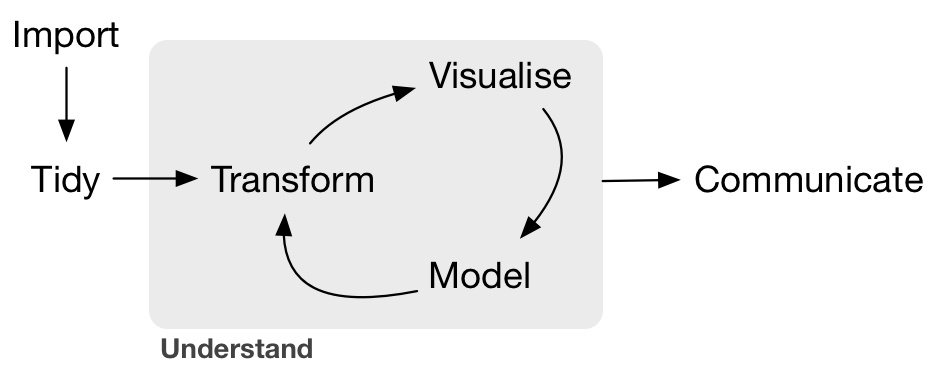
\includegraphics[width=13.01in]{images/tidy1} 

}

\caption{Data/Science Pipeline}\label{fig:pipeline-figure}
\end{figure}

\begin{center}\rule{0.5\linewidth}{0.5pt}\end{center}

\hypertarget{inspirations-and-references}{%
\section{Inspirations and references}\label{inspirations-and-references}}

Basically, the book combines my (Katrien Antonio) own research papers and coursenotes with many useful quotes and examples from my favourite R books listed below.

This book is very much inspired by the following books or courses:

\begin{itemize}
\tightlist
\item
  ``Mathematical Statistics with Resampling and R'' (Chihara and Hesterberg 2011),
\item
  ``OpenIntro: Intro Stat with Randomization and Simulation'' (Diez, Barr, and Çetinkaya-Rundel 2014), and
\item
  ``R for Data Science'' (Grolemund and Wickham 2016),
\item
  ``Moderndive'' (Ismay and Kim 2018),
\item
  Jared Lander's ``R for everyone'' (Lander 2017)
\item
  ``Applied Econometrics with R'' (Kleiber and Zeileis 2008)
\item
  ``An Introduction to Statistical Learning'' (James et al. 20AD)
\item
  all the work of Michael Clark, see \href{http://m-clark.github.io/cv.html}{Michael Clark's website}
  - many, many courses on the \href{www.datacamp.com}{DataCamp} platform, including Katrien Antonio and Roel Verbelen's \href{https://www.datacamp.com/courses/2333}{Valuation of Life Insurance Products in R}.
\end{itemize}

\begin{center}\rule{0.5\linewidth}{0.5pt}\end{center}

\hypertarget{sec:about-book}{%
\section{About this book}\label{sec:about-book}}

This book was written using RStudio's \href{https://bookdown.org/}{bookdown} package by Yihui Xie (Xie 2020). This package simplifies the publishing of books by having all content written in \href{http://rmarkdown.rstudio.com/html_document_format.html}{R Markdown}. The bookdown/R Markdown source code for all versions of ModernDive is available on GitHub.

Could this be a new paradigm for textbooks? Instead of the traditional model of textbook companies publishing updated \emph{editions} of the textbook every few years, we apply a software design influenced model of publishing more easily updated \emph{versions}. We can then leverage open-source communities of instructors and developers for ideas, tools, resources, and feedback. As such, we welcome your pull requests.

Finally, feel free to modify the book as you wish for your own needs, but please list the authors at the top of \texttt{index.Rmd} as ``Chester Ismay, Albert Y. Kim, and YOU!'' \textbf{So, that is exactly what Katrien Antonio did!}

\begin{center}\rule{0.5\linewidth}{0.5pt}\end{center}

\hypertarget{getting-started}{%
\chapter{Getting started in R}\label{getting-started}}

Before we can start exploring data in R, there are some key concepts to understand first:

\begin{enumerate}
\def\labelenumi{\arabic{enumi}.}
\tightlist
\item
  What are R and RStudio?
\item
  How do I code in R?
\item
  What are R packages?
\end{enumerate}

Much of this chapter is based on two sources which you should feel free to use as references if you are looking for additional details:

\begin{enumerate}
\def\labelenumi{\arabic{enumi}.}
\tightlist
\item
  Ismay's \href{http://ismayc.github.io/rbasics-book}{Getting used to R, RStudio, and R Markdown} (Ismay 2016), which includes video screen recordings that you can follow along and pause as you learn.
\item
  DataCamp's online tutorials. DataCamp is a browser-based interactive platform for learning data science and their tutorials will help facilitate your learning of the above concepts (and other topics in this book). Go to \href{https://www.datacamp.com/}{DataCamp} and create an account before continuing.
\end{enumerate}

\begin{center}\rule{0.5\linewidth}{0.5pt}\end{center}

\hypertarget{some-history}{%
\section{Some history}\label{some-history}}

R is a dialect of the S language (developed by John Chambers at Bell Labs in the 70s), namely `Gnu-S'. R was written by Robert Gentleman and Ross Ihaka (while being at the University of Auckland) in 1993.

\begin{center}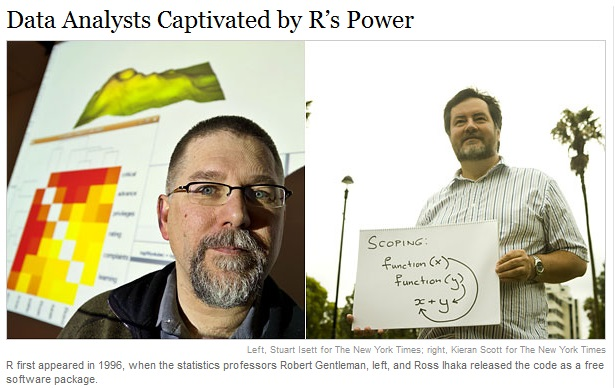
\includegraphics[width=8.54in]{images/NYTimesR2009} \end{center}

The (Kleiber and Zeileis 2008) book sketches the history of R, in Sections 1.5 and 1.6. The R source code was first released under the GNU General Public License (GPL) in 1995. Since mid-1997, there has been the R Development Core Team, currently comprising 20 members. In 1998, the Comprehensive R Archive Network \href{http://CRAN.R-project.org/}{CRAN} was established, a family of mirror sites around the world that store identical, up-to-date versions of code and documentation for R. The first official release, R version 1.0.0, dates to 2000-02-29. Currently, version 3.5.0 is available.

R is open source, i.e.~\href{http://en.wikipedia.org/wiki/GNU_General_Public_License}{GNU General Public License}. The R environment (see \href{http://www.r-project.org/about.html}{About R}) is `an integrated suite of software facilities for data manipulation, calculation and graphical display'.

\hypertarget{what-are-r-and-rstudio}{%
\section{What are R and RStudio?}\label{what-are-r-and-rstudio}}

For much of this book, we will assume that you are using R via RStudio. First time users often confuse the two. At its simplest:

\begin{itemize}
\tightlist
\item
  R is like a car's engine
\item
  RStudio is like a car's dashboard
\end{itemize}

\begin{longtable}[]{@{}cc@{}}
\toprule
R: Engine & RStudio: Dashboard\tabularnewline
\midrule
\endhead
&\tabularnewline
\bottomrule
\end{longtable}

More precisely, R is a programming language that runs computations while RStudio is an \emph{integrated development environment (IDE)} that provides an interface by adding many convenient features and tools. So the way of having access to a speedometer, rearview mirrors, and a navigation system makes driving much easier, using RStudio's interface makes using R much easier as well.

Optional: For a more in-depth discussion on the difference between R and RStudio IDE, watch this \href{https://campus.datacamp.com/courses/working-with-the-rstudio-ide-part-1/orientation?ex=1}{DataCamp video (2m52s)}.

\hypertarget{installing-r-and-rstudio}{%
\subsection{Installing R and RStudio}\label{installing-r-and-rstudio}}

You will first need to download and install both R and RStudio (Desktop version) on your computer.

\begin{enumerate}
\def\labelenumi{\arabic{enumi}.}
\tightlist
\item
  \href{https://cran.r-project.org/}{Download and install R}.
\end{enumerate}

\begin{itemize}
\tightlist
\item
  Note: You must do this first.
\item
  Click on the download link corresponding to your computer's operating system.
\end{itemize}

\begin{enumerate}
\def\labelenumi{\arabic{enumi}.}
\tightlist
\item
  \href{https://www.rstudio.com/products/rstudio/download3/}{Download and install RStudio}.
\end{enumerate}

\begin{itemize}
\tightlist
\item
  Scroll down to ``Installers for Supported Platforms''
\item
  Click on the download link corresponding to your computer's operating system.
\end{itemize}

Optional: If you need more detailed instructions on how to install R and RStudio, watch this \href{https://campus.datacamp.com/courses/working-with-the-rstudio-ide-part-1/orientation?ex=3}{DataCamp video (1m22s)}.

\hypertarget{using-r-via-rstudio}{%
\subsection{Using R via RStudio}\label{using-r-via-rstudio}}

Recall our car analogy from above. Much as we don't drive a car by interacting directly with the engine but rather by using elements on the car's dashboard, we won't be using R directly but rather we will use RStudio's interface. After you install R and RStudio on your computer, you'll have two new programs AKA applications you can open. We will always work in RStudio and not R. In other words:

\begin{longtable}[]{@{}cc@{}}
\toprule
R: Do not open this & RStudio: Open this\tabularnewline
\midrule
\endhead
&\tabularnewline
\bottomrule
\end{longtable}

After you open RStudio, you should see the following:

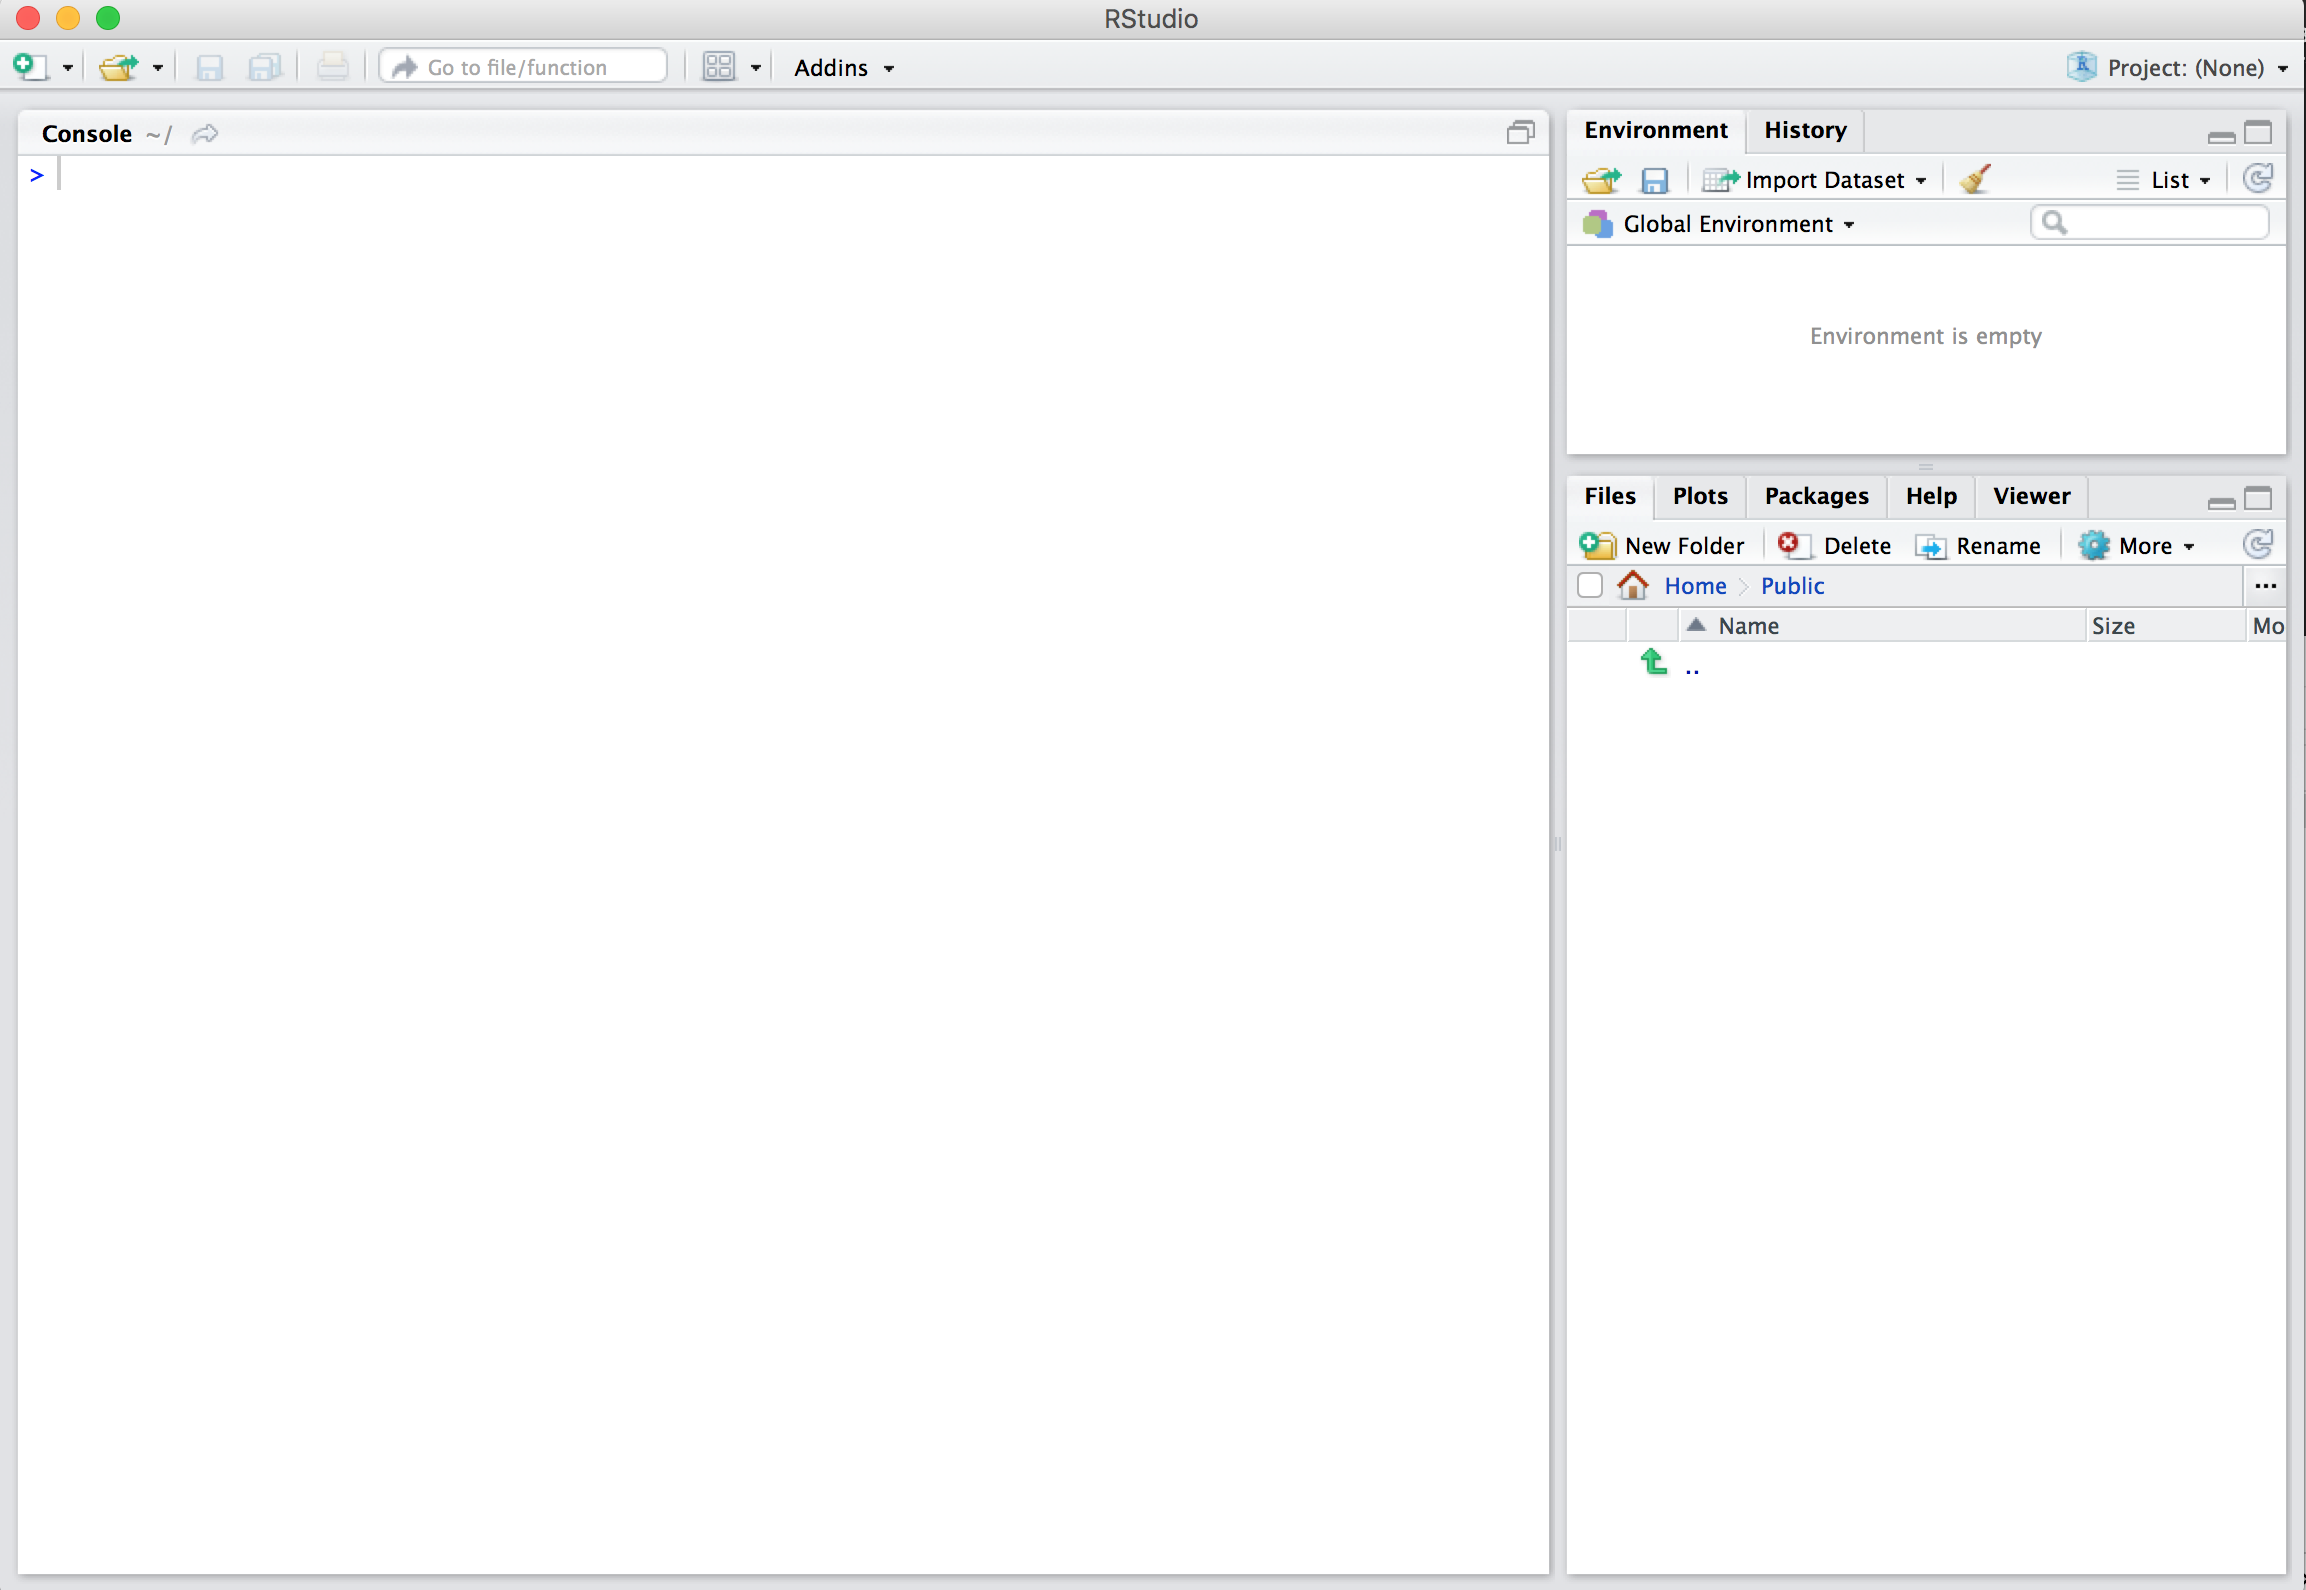
\includegraphics{images/rstudio.png}

Watch the following \href{https://campus.datacamp.com/courses/working-with-the-rstudio-ide-part-1/orientation?ex=5}{DataCamp video (4m10s)} to learn about the different \emph{panes} in RStudio, in particular the \emph{Console pane} where you will later run R code.

\begin{center}\rule{0.5\linewidth}{0.5pt}\end{center}

\hypertarget{code}{%
\section{How do I code in R?}\label{code}}

Now that you're set up with R and RStudio, you are probably asking yourself ``OK. Now how do I use R?'' The first thing to note as that unlike other software like Excel, STATA, or SAS that provide \href{https://en.wikipedia.org/wiki/Point_and_click}{point and click} interfaces, R is an \href{https://en.wikipedia.org/wiki/Interpreted_language}{interpreted language}, meaning you have to enter in R commands written in R code i.e.~you have to program in R (we use the terms ``coding'' and ``programming'' interchangeably in this book).

While it is not required to be a seasoned coder/computer programmer to use R, there is still a set of basic programming concepts that R users need to understand. Consequently, while this book is not a book on programming, you will still learn just enough of these basic programming concepts needed to explore and analyze data effectively.

\hypertarget{tips-on-learning-to-code}{%
\subsection{Tips on learning to code}\label{tips-on-learning-to-code}}

Learning to code/program is very much like learning a foreign language, it can be very daunting and frustrating at first. However just as with learning a foreign language, if you put in the effort and are not afraid to make mistakes, anybody can learn. Lastly, there are a few useful things to keep in mind as you learn to program:

\begin{itemize}
\tightlist
\item
  \textbf{Computers are stupid}: You have to tell a computer everything it needs to do. Furthermore, your instructions can't have any mistakes in them, nor can they be ambiguous in any way.
\item
  \textbf{Take the ``copy/paste/tweak'' approach}: Especially when learning your first programming language, it is often much easier to taking existing code that you know works and modify it to suit your ends, rather than trying to write new code from scratch. We call this the \emph{copy/paste/tweak} approach. So early on, we suggest not trying to code from scratch, but please take the code we provide throughout this book and play around with it!
\item
  \textbf{Practice is key}: Just as the only solution to improving your foreign language skills is practice, so also the only way to get better at R is through pracitice. Don't worry however, we'll give you plenty of opportunities to practice!
\end{itemize}

\begin{center}\rule{0.5\linewidth}{0.5pt}\end{center}

\hypertarget{packages}{%
\section{What are R packages?}\label{packages}}

Another point of confusion with new R users is the notion of a package. R packages extend the functionality of R by providing additional functions, data, and documentation and can be downloaded for free from the internet. They are written by a world-wide community of R users. For example, among the many packages we will use in this book are the

\begin{itemize}
\tightlist
\item
  \texttt{ggplot2} package for data visualization in Chapter \ref{data-viz}
\item
  \texttt{dplyr} package for data wrangling in Chapter \ref{data-wrangling}
\end{itemize}

There are two key things to remember about R packages:

\begin{enumerate}
\def\labelenumi{\arabic{enumi}.}
\tightlist
\item
  \emph{Installation}: Most packages are not installed by default when you install R and RStudio. You need to install a package before you can use it. Once you've installed it, you likely don't need to install it again unless you want to update it to a newer version of the package.
\item
  \emph{Loading}: Packages are not loaded automatically when you open RStudio. You need to load them everytime you open RStudio using the \texttt{library()} command.
\end{enumerate}

A good analogy for R packages is they are like apps you can download onto a mobile phone:

\begin{longtable}[]{@{}cc@{}}
\toprule
R: A new phone & R Packages: Apps you can download\tabularnewline
\midrule
\endhead
&\tabularnewline
\bottomrule
\end{longtable}

So, expanding on this analogy a bit:

\begin{enumerate}
\def\labelenumi{\arabic{enumi}.}
\tightlist
\item
  R is like a new mobile phone. It has a certain amount of functionality when you use it for the first time, but it doesn't have everything.
\item
  R packages are like the apps you can download onto your phone, much like those offered in the App Store and Google Play. For example: Instagram.
\item
  In order to use a package, just like in order to use Instagram, you must:
\item
  First download it and install it. You do this only once.
\item
  Load it, or in other words, ``open'' it, using the \texttt{library()} command.
\end{enumerate}

So just as you can only start sharing photos with your friends on Instagram if you first install the app and then open it, you can only access an R package's data and functions if you first install the package and then load it with the \texttt{library()} command. Let's cover these two steps:

\hypertarget{package-installation}{%
\subsection{Package installation}\label{package-installation}}

(Note that if you are working on an RStudio Server, you probably will not need to install your own packages as that has been already done for you. Still it is important that you know this process for later when you are not using the RStudio Server but rather your own installation of RStudio Desktop.)

There are two ways to install an R package. For example, to install the \texttt{ggplot2} package:

\begin{enumerate}
\def\labelenumi{\arabic{enumi}.}
\tightlist
\item
  \textbf{Easy way}: In the Files pane of RStudio:
\end{enumerate}

\begin{enumerate}
\def\labelenumi{\alph{enumi})}
\tightlist
\item
  Click on the ``Packages'' tab
\item
  Click on ``Install''
\item
  Type the name of the package under ``Packages (separate multiple with space or comma):'' In this case, type \texttt{ggplot2}
\item
  Click ``Install''
\end{enumerate}

\begin{enumerate}
\def\labelenumi{\arabic{enumi}.}
\tightlist
\item
  \textbf{Alternative way}: In the Console pane run \texttt{install.packages("ggplot2")} (you must include the quotation marks).
\end{enumerate}

Repeat this for the \texttt{dplyr} and \texttt{nycflights13} packages. If you still experience problems, have a look at this blog post \href{https://www.r-bloggers.com/installing-r-packages/}{Installing R packages}.

\textbf{Note}: You only have to install a package once, unless you want to update an already installed package to the latest version. If you want to update a package to the latest version, then re-install it by repeating the above steps.

\hypertarget{package-loading}{%
\subsection{Package loading}\label{package-loading}}

After you've installed a package, you can now load it using the \texttt{library()} command. For example, to load the \texttt{ggplot2} and \texttt{dplyr} packages, run the following code in the Console pane:

\begin{Shaded}
\begin{Highlighting}[]
\KeywordTok{library}\NormalTok{(ggplot2)}
\KeywordTok{library}\NormalTok{(dplyr)}
\end{Highlighting}
\end{Shaded}

\textbf{Note}: You have to reload each package you want to use every time you open a new session of RStudio. This is a little annoying to get used to and will be your most common error as you begin. When you see an error such as

\begin{verbatim}
Error: could not find function
\end{verbatim}

remember that this likely comes from you trying to use a function in a package that has not been loaded. Remember to run the \texttt{library()} function with the appropriate package to fix this error.

\hypertarget{packages-on-cran}{%
\subsection{Packages on CRAN}\label{packages-on-cran}}

R comes with a set of \texttt{base} packages or \texttt{base} system, maintained by the R core
team only. Examples: \texttt{base}, \texttt{datasets}, \texttt{graphics}. Additional packages are on CRAN (Thursday 1/23/2014: 5,140
packages; Sunday 9/7/2014: 5,852 packages; Saturday 11/08/2014:
6,041 packages; Tuesday 11/8/2016: 9,473 packages; Monday
12/04/2017: 11,946 packages; Tuesday 04/10/2018: 12,430
packages). These packages are developed and maintained by R users worldwide,
and shared with the R community through CRAN.

\begin{center}\rule{0.5\linewidth}{0.5pt}\end{center}

\hypertarget{conclusion}{%
\section{Conclusion}\label{conclusion}}

You are now ready to get start your journey as an R-enthusiast!

\begin{center}\rule{0.5\linewidth}{0.5pt}\end{center}

\hypertarget{objects-data-types}{%
\chapter{Objects and data types in R}\label{objects-data-types}}

\hypertarget{how-it-works}{%
\section{How it works}\label{how-it-works}}

You will now start with writing R code in the console and you will explore a first script of R code. Every line of code is interpreted and executed by R and you get a message whether or not your code was correct. The output of your R code is then shown in the console.
R makes use of the \# sign to add comments, so that you and others can understand what the R code is about. Just like Twitter! Comments are not run as R code, so they will not influence your result. {[}Quote from DataCamp's `Introduction to R' course.{]} In its most basic form, R can be used as a simple calculator. We illustrate the use of some arithmetic operators in the code below.

\begin{Shaded}
\begin{Highlighting}[]
\CommentTok{# use 'right click, run line or selection', of Ctrl+R}
\DecValTok{10}\OperatorTok{^}\DecValTok{2}\OperatorTok{+}\DecValTok{36}
\end{Highlighting}
\end{Shaded}

\begin{verbatim}
[1] 136
\end{verbatim}

\begin{center}\rule{0.5\linewidth}{0.5pt}\end{center}

\hypertarget{variables}{%
\section{Variables}\label{variables}}

A basic concept in (statistical) programming is called a \emph{variable}.
A variable allows you to store a value (e.g.~4) or an object (e.g.~a function description) in R. You can then later use this variable's name to easily access the value or the object that is stored within this variable. {[}Quote from DataCamp's `Introduction to R' course.{]}

\begin{Shaded}
\begin{Highlighting}[]
\CommentTok{# assign value '4' to 'a'}
\NormalTok{a <-}\StringTok{ }\DecValTok{4}
\NormalTok{a}
\end{Highlighting}
\end{Shaded}

\begin{verbatim}
[1] 4
\end{verbatim}

\begin{Shaded}
\begin{Highlighting}[]
\CommentTok{# now R remembers what 'a' is}
\CommentTok{# calculations with 'a'}
\NormalTok{a}\OperatorTok{*}\DecValTok{5}
\end{Highlighting}
\end{Shaded}

\begin{verbatim}
[1] 20
\end{verbatim}

\begin{Shaded}
\begin{Highlighting}[]
\NormalTok{(a}\OperatorTok{+}\DecValTok{10}\NormalTok{)}\OperatorTok{/}\DecValTok{2}
\end{Highlighting}
\end{Shaded}

\begin{verbatim}
[1] 7
\end{verbatim}

\begin{Shaded}
\begin{Highlighting}[]
\CommentTok{# or give a new value to 'a'}
\NormalTok{a <-}\StringTok{ }\NormalTok{a}\OperatorTok{+}\DecValTok{1}
\NormalTok{a}
\end{Highlighting}
\end{Shaded}

\begin{verbatim}
[1] 5
\end{verbatim}

\begin{center}\rule{0.5\linewidth}{0.5pt}\end{center}

\hypertarget{basic-data-types}{%
\section{Basic data types}\label{basic-data-types}}

R works with numerous data types. Some of the most basic types to get started are:

\begin{itemize}
\tightlist
\item
  Decimal values like 4.5 are called numerics.
\item
  Natural numbers like 4 are called integers. Integers are also numerics.
\item
  Boolean values (TRUE or FALSE) are called logical.
\item
  Dates or \texttt{POSIXct} for time based variables. Here, \texttt{Date} stores just a date and \texttt{POSIXct} stores a date and time. Both objects are actually represented as the number of days (Date) or seconds (POSIXct) since January 1, 1970.
\item
  Text (or string) values are called characters.
\end{itemize}

Note how the quotation marks on the right indicate that ``some text'' is a character.

\begin{Shaded}
\begin{Highlighting}[]
\NormalTok{my_numeric <-}\StringTok{ }\FloatTok{42.5}

\NormalTok{my_character <-}\StringTok{ "some text"}

\NormalTok{my_logical <-}\StringTok{ }\OtherTok{TRUE}

\NormalTok{my_date <-}\StringTok{ }\KeywordTok{as.Date}\NormalTok{(}\StringTok{"05/29/2018"}\NormalTok{, }\StringTok{"%m/%d/%Y"}\NormalTok{)}
\end{Highlighting}
\end{Shaded}

You can check the data type of a variable beforehand. You can do this with the class() function.

\begin{Shaded}
\begin{Highlighting}[]
\KeywordTok{class}\NormalTok{(my_numeric)}
\end{Highlighting}
\end{Shaded}

\begin{verbatim}
[1] "numeric"
\end{verbatim}

\begin{Shaded}
\begin{Highlighting}[]
\CommentTok{# your turn to check the type of 'my_character' and 'my_logical' and 'my_date'}
\end{Highlighting}
\end{Shaded}

\begin{center}\rule{0.5\linewidth}{0.5pt}\end{center}

\hypertarget{everything-is-an-object}{%
\section{Everything is an object}\label{everything-is-an-object}}

In R, an analysis is normally broken down into a series
of steps. Intermediate results are stored in objects, with minimal output at
each step (often none). Instead, the objects are further manipulated to obtain
the information required. In fact, the fundamental design principle underlying R (and S) is ``everything
is an object''. Hence, not only vectors and matrices are objects that
can be passed to and returned by functions, but also functions themselves,
and even function calls. (Quote from `Applied Econometrics in R', by Kleiber \& Zeileis) A variable in R can take on any available data type, or hold any R object.

\begin{Shaded}
\begin{Highlighting}[]
\CommentTok{# see all objects stored in R's memory, where 'ls()' is for 'List Objects' }
\CommentTok{# and returns a vector of character strings}
\CommentTok{# giving the names of the objects in the specified environment}
\KeywordTok{ls}\NormalTok{()}
\end{Highlighting}
\end{Shaded}

\begin{verbatim}
[1] "a"            "my_character" "my_date"      "my_logical"   "my_numeric"  
[6] "needed_pkgs"  "new_pkgs"    
\end{verbatim}

\begin{Shaded}
\begin{Highlighting}[]
\CommentTok{# to remove objects from R's memory, use}
\KeywordTok{rm}\NormalTok{(a)}
\KeywordTok{rm}\NormalTok{(my_character, my_logical)}
\KeywordTok{rm}\NormalTok{(}\DataTypeTok{list=}\KeywordTok{c}\NormalTok{(}\StringTok{'my_date'}\NormalTok{, }\StringTok{'my_numeric'}\NormalTok{))}
\KeywordTok{rm}\NormalTok{(}\DataTypeTok{list=}\KeywordTok{ls}\NormalTok{())}
\end{Highlighting}
\end{Shaded}

\begin{center}\rule{0.5\linewidth}{0.5pt}\end{center}

\hypertarget{vectors}{%
\section{Vectors}\label{vectors}}

Vectors are one-dimension arrays that can hold numeric data, character data, or logical data. In other words, a vector is a simple tool to store data. In R, you create a vector with the combine function c(). You place the vector elements separated by a comma between the parentheses. (Quote from DataCamp's `Introduction to R course') Vectors are key! Operations are applied to each element of the vector automatically, there is no need to loop through the vector.

\begin{Shaded}
\begin{Highlighting}[]
\CommentTok{# To combine elements into a vector, use c():}
\KeywordTok{c}\NormalTok{(}\DecValTok{1}\NormalTok{, }\DecValTok{2}\NormalTok{, }\DecValTok{3}\NormalTok{, }\DecValTok{4}\NormalTok{)}
\end{Highlighting}
\end{Shaded}

\begin{verbatim}
[1] 1 2 3 4
\end{verbatim}

\begin{Shaded}
\begin{Highlighting}[]
\CommentTok{# or}
\DecValTok{1}\OperatorTok{:}\DecValTok{10}
\end{Highlighting}
\end{Shaded}

\begin{verbatim}
 [1]  1  2  3  4  5  6  7  8  9 10
\end{verbatim}

\begin{Shaded}
\begin{Highlighting}[]
\CommentTok{# or}
\KeywordTok{seq}\NormalTok{(}\DataTypeTok{from=}\DecValTok{0}\NormalTok{, }\DataTypeTok{to=}\DecValTok{10}\NormalTok{, }\DataTypeTok{by=}\FloatTok{0.5}\NormalTok{)}
\end{Highlighting}
\end{Shaded}

\begin{verbatim}
 [1]  0.0  0.5  1.0  1.5  2.0  2.5  3.0  3.5  4.0  4.5  5.0  5.5  6.0  6.5  7.0
[16]  7.5  8.0  8.5  9.0  9.5 10.0
\end{verbatim}

\begin{Shaded}
\begin{Highlighting}[]
\CommentTok{# create a variable x}
\NormalTok{x <-}\StringTok{ }\DecValTok{1}\OperatorTok{:}\DecValTok{20}
\NormalTok{x}
\end{Highlighting}
\end{Shaded}

\begin{verbatim}
 [1]  1  2  3  4  5  6  7  8  9 10 11 12 13 14 15 16 17 18 19 20
\end{verbatim}

\begin{Shaded}
\begin{Highlighting}[]
\NormalTok{x[}\DecValTok{6}\OperatorTok{:}\DecValTok{9}\NormalTok{]}
\end{Highlighting}
\end{Shaded}

\begin{verbatim}
[1] 6 7 8 9
\end{verbatim}

\begin{Shaded}
\begin{Highlighting}[]
\NormalTok{x[}\KeywordTok{c}\NormalTok{(}\DecValTok{2}\NormalTok{, }\DecValTok{5}\NormalTok{, }\DecValTok{13}\NormalTok{)]}
\end{Highlighting}
\end{Shaded}

\begin{verbatim}
[1]  2  5 13
\end{verbatim}

\begin{Shaded}
\begin{Highlighting}[]
\CommentTok{# or}
\NormalTok{xx <-}\StringTok{ }\KeywordTok{c}\NormalTok{(}\DecValTok{0}\NormalTok{, }\DecValTok{3}\OperatorTok{:}\DecValTok{5}\NormalTok{, }\DecValTok{20}\NormalTok{, }\DecValTok{0}\NormalTok{)}
\NormalTok{xx}
\end{Highlighting}
\end{Shaded}

\begin{verbatim}
[1]  0  3  4  5 20  0
\end{verbatim}

\begin{Shaded}
\begin{Highlighting}[]
\NormalTok{xx[}\DecValTok{2}\OperatorTok{:}\DecValTok{3}\NormalTok{]}
\end{Highlighting}
\end{Shaded}

\begin{verbatim}
[1] 3 4
\end{verbatim}

\begin{Shaded}
\begin{Highlighting}[]
\KeywordTok{length}\NormalTok{(xx)}
\end{Highlighting}
\end{Shaded}

\begin{verbatim}
[1] 6
\end{verbatim}

\begin{Shaded}
\begin{Highlighting}[]
\CommentTok{# but c(.) can also concatenate other things than numbers}
\NormalTok{family <-}\StringTok{ }\KeywordTok{c}\NormalTok{(}\StringTok{"Katrien"}\NormalTok{, }\StringTok{"Jan"}\NormalTok{, }\StringTok{"Leen"}\NormalTok{)}
\NormalTok{family}
\end{Highlighting}
\end{Shaded}

\begin{verbatim}
[1] "Katrien" "Jan"     "Leen"   
\end{verbatim}

\begin{Shaded}
\begin{Highlighting}[]
\NormalTok{family[}\DecValTok{2}\NormalTok{]}
\end{Highlighting}
\end{Shaded}

\begin{verbatim}
[1] "Jan"
\end{verbatim}

\begin{Shaded}
\begin{Highlighting}[]
\KeywordTok{str}\NormalTok{(family) }\CommentTok{# str() displays the structure of an R object in compact way}
\end{Highlighting}
\end{Shaded}

\begin{verbatim}
 chr [1:3] "Katrien" "Jan" "Leen"
\end{verbatim}

\begin{Shaded}
\begin{Highlighting}[]
\KeywordTok{class}\NormalTok{(family)}
\end{Highlighting}
\end{Shaded}

\begin{verbatim}
[1] "character"
\end{verbatim}

You can give a name to the elements of a vector with the \texttt{names()} function. Here is how it works

\begin{Shaded}
\begin{Highlighting}[]
\NormalTok{my_vector <-}\StringTok{ }\KeywordTok{c}\NormalTok{(}\StringTok{"Katrien Antonio"}\NormalTok{, }\StringTok{"teacher"}\NormalTok{)}
\KeywordTok{names}\NormalTok{(my_vector) <-}\StringTok{ }\KeywordTok{c}\NormalTok{(}\StringTok{"Name"}\NormalTok{, }\StringTok{"Profession"}\NormalTok{)}
\NormalTok{my_vector}
\end{Highlighting}
\end{Shaded}

\begin{verbatim}
             Name        Profession 
"Katrien Antonio"         "teacher" 
\end{verbatim}

\begin{center}\rule{0.5\linewidth}{0.5pt}\end{center}

\hypertarget{matrices}{%
\section{Matrices}\label{matrices}}

In R, a matrix is a collection of elements of the same data type (numeric, character, or logical) arranged into a fixed number of rows and columns. Since you are only working with rows and columns, a matrix is called two-dimensional. You can construct a matrix in R with the \texttt{matrix()} function. (Quote from DataCamp's `Introduction to R course')

\begin{Shaded}
\begin{Highlighting}[]
\CommentTok{# a 3x4 matrix, filled with 1,2,..., 12}
\KeywordTok{matrix}\NormalTok{(}\DecValTok{1}\OperatorTok{:}\DecValTok{12}\NormalTok{, }\DecValTok{3}\NormalTok{, }\DecValTok{4}\NormalTok{, }\DataTypeTok{byrow =} \OtherTok{TRUE}\NormalTok{)}
\end{Highlighting}
\end{Shaded}

\begin{verbatim}
     [,1] [,2] [,3] [,4]
[1,]    1    2    3    4
[2,]    5    6    7    8
[3,]    9   10   11   12
\end{verbatim}

\begin{Shaded}
\begin{Highlighting}[]
\KeywordTok{matrix}\NormalTok{(}\DecValTok{1}\OperatorTok{:}\DecValTok{12}\NormalTok{, }\DataTypeTok{byrow =} \OtherTok{TRUE}\NormalTok{, }\DataTypeTok{nrow=}\DecValTok{3}\NormalTok{)}
\end{Highlighting}
\end{Shaded}

\begin{verbatim}
     [,1] [,2] [,3] [,4]
[1,]    1    2    3    4
[2,]    5    6    7    8
[3,]    9   10   11   12
\end{verbatim}

\begin{Shaded}
\begin{Highlighting}[]
\CommentTok{# hmmm, check help on 'matrix'}
\NormalTok{? matrix}
\end{Highlighting}
\end{Shaded}

\begin{verbatim}
starting httpd help server ... done
\end{verbatim}

\begin{Shaded}
\begin{Highlighting}[]
\CommentTok{# one way of creating matrices is to bind vectors together}
\KeywordTok{cbind}\NormalTok{(}\DecValTok{1}\OperatorTok{:}\DecValTok{2}\NormalTok{, }\DecValTok{6}\OperatorTok{:}\DecValTok{9}\NormalTok{)     }\CommentTok{# by columns}
\end{Highlighting}
\end{Shaded}

\begin{verbatim}
     [,1] [,2]
[1,]    1    6
[2,]    2    7
[3,]    1    8
[4,]    2    9
\end{verbatim}

\begin{Shaded}
\begin{Highlighting}[]
\KeywordTok{rbind}\NormalTok{(}\DecValTok{1}\OperatorTok{:}\DecValTok{3}\NormalTok{, }\OperatorTok{-}\NormalTok{(}\DecValTok{1}\OperatorTok{:}\DecValTok{3}\NormalTok{))  }\CommentTok{# by rows}
\end{Highlighting}
\end{Shaded}

\begin{verbatim}
     [,1] [,2] [,3]
[1,]    1    2    3
[2,]   -1   -2   -3
\end{verbatim}

\begin{Shaded}
\begin{Highlighting}[]
\CommentTok{# create matrix object 'm'}
\NormalTok{m <-}\StringTok{ }\KeywordTok{matrix}\NormalTok{(}\DecValTok{1}\OperatorTok{:}\DecValTok{12}\NormalTok{, }\DecValTok{3}\NormalTok{, }\DecValTok{4}\NormalTok{)}
\NormalTok{m}
\end{Highlighting}
\end{Shaded}

\begin{verbatim}
     [,1] [,2] [,3] [,4]
[1,]    1    4    7   10
[2,]    2    5    8   11
[3,]    3    6    9   12
\end{verbatim}

\begin{Shaded}
\begin{Highlighting}[]
\NormalTok{m[}\DecValTok{1}\NormalTok{,}\DecValTok{4}\NormalTok{] }\CommentTok{# extract an element}
\end{Highlighting}
\end{Shaded}

\begin{verbatim}
[1] 10
\end{verbatim}

\begin{Shaded}
\begin{Highlighting}[]
\NormalTok{m[,}\DecValTok{2}\NormalTok{]  }\CommentTok{# extract a column}
\end{Highlighting}
\end{Shaded}

\begin{verbatim}
[1] 4 5 6
\end{verbatim}

\begin{Shaded}
\begin{Highlighting}[]
\KeywordTok{nrow}\NormalTok{(m);}\KeywordTok{ncol}\NormalTok{(m);}\KeywordTok{dim}\NormalTok{(m) }\CommentTok{# useful stuff}
\end{Highlighting}
\end{Shaded}

\begin{verbatim}
[1] 3
\end{verbatim}

\begin{verbatim}
[1] 4
\end{verbatim}

\begin{verbatim}
[1] 3 4
\end{verbatim}

\begin{Shaded}
\begin{Highlighting}[]
\CommentTok{# another example}
\NormalTok{m <-}\StringTok{ }\KeywordTok{cbind}\NormalTok{(}\DataTypeTok{a =} \DecValTok{1}\OperatorTok{:}\DecValTok{3}\NormalTok{, }\DataTypeTok{b =}\NormalTok{ letters[}\DecValTok{1}\OperatorTok{:}\DecValTok{3}\NormalTok{])}
\NormalTok{m}
\end{Highlighting}
\end{Shaded}

\begin{verbatim}
     a   b  
[1,] "1" "a"
[2,] "2" "b"
[3,] "3" "c"
\end{verbatim}

\begin{Shaded}
\begin{Highlighting}[]
\CommentTok{# ask help, what is the built-in 'letters'?}
\NormalTok{? letters}
\end{Highlighting}
\end{Shaded}

\begin{center}\rule{0.5\linewidth}{0.5pt}\end{center}

\hypertarget{data-frames}{%
\section{Data frames}\label{data-frames}}

Most data sets you will be working with will be stored as data frames. A data frame has the variables of a data set as columns and the observations as rows. This will be a familiar concept for those coming from different statistical software packages such as SAS or SPSS.

First, you will look at a `classic' data set from the \texttt{datasets} package that comes with the base R installation. The \texttt{mtcars} (Motor Trend Car Road Tests) data was extracted from the 1974 Motor Trend US magazine, and comprises fuel consumption and 10 aspects of automobile design and performance for 32 automobiles (1973-74 models). (Quote from DataCamp's `Introduction to R course')

\begin{Shaded}
\begin{Highlighting}[]
\NormalTok{mtcars}
\end{Highlighting}
\end{Shaded}

\begin{Shaded}
\begin{Highlighting}[]
\KeywordTok{str}\NormalTok{(mtcars)}
\end{Highlighting}
\end{Shaded}

\begin{verbatim}
'data.frame':	32 obs. of  11 variables:
 $ mpg : num  21 21 22.8 21.4 18.7 18.1 14.3 24.4 22.8 19.2 ...
 $ cyl : num  6 6 4 6 8 6 8 4 4 6 ...
 $ disp: num  160 160 108 258 360 ...
 $ hp  : num  110 110 93 110 175 105 245 62 95 123 ...
 $ drat: num  3.9 3.9 3.85 3.08 3.15 2.76 3.21 3.69 3.92 3.92 ...
 $ wt  : num  2.62 2.88 2.32 3.21 3.44 ...
 $ qsec: num  16.5 17 18.6 19.4 17 ...
 $ vs  : num  0 0 1 1 0 1 0 1 1 1 ...
 $ am  : num  1 1 1 0 0 0 0 0 0 0 ...
 $ gear: num  4 4 4 3 3 3 3 4 4 4 ...
 $ carb: num  4 4 1 1 2 1 4 2 2 4 ...
\end{verbatim}

\begin{Shaded}
\begin{Highlighting}[]
\KeywordTok{head}\NormalTok{(mtcars)}
\end{Highlighting}
\end{Shaded}

\begin{verbatim}
                   mpg cyl disp  hp drat    wt  qsec vs am gear carb
Mazda RX4         21.0   6  160 110 3.90 2.620 16.46  0  1    4    4
Mazda RX4 Wag     21.0   6  160 110 3.90 2.875 17.02  0  1    4    4
Datsun 710        22.8   4  108  93 3.85 2.320 18.61  1  1    4    1
Hornet 4 Drive    21.4   6  258 110 3.08 3.215 19.44  1  0    3    1
Hornet Sportabout 18.7   8  360 175 3.15 3.440 17.02  0  0    3    2
Valiant           18.1   6  225 105 2.76 3.460 20.22  1  0    3    1
\end{verbatim}

\begin{Shaded}
\begin{Highlighting}[]
\KeywordTok{tail}\NormalTok{(mtcars)}
\end{Highlighting}
\end{Shaded}

\begin{verbatim}
                mpg cyl  disp  hp drat    wt qsec vs am gear carb
Porsche 914-2  26.0   4 120.3  91 4.43 2.140 16.7  0  1    5    2
Lotus Europa   30.4   4  95.1 113 3.77 1.513 16.9  1  1    5    2
Ford Pantera L 15.8   8 351.0 264 4.22 3.170 14.5  0  1    5    4
Ferrari Dino   19.7   6 145.0 175 3.62 2.770 15.5  0  1    5    6
Maserati Bora  15.0   8 301.0 335 3.54 3.570 14.6  0  1    5    8
Volvo 142E     21.4   4 121.0 109 4.11 2.780 18.6  1  1    4    2
\end{verbatim}

Since using built-in data sets is not even half the fun of creating your own data sets, you will now work with your own personally created data set. (Quote from DataCamp's `Introduction to R course')

\begin{Shaded}
\begin{Highlighting}[]
\NormalTok{t <-}\StringTok{ }\KeywordTok{data.frame}\NormalTok{(}\DataTypeTok{x =} \KeywordTok{c}\NormalTok{(}\DecValTok{11}\NormalTok{, }\DecValTok{12}\NormalTok{, }\DecValTok{7}\NormalTok{), }\DataTypeTok{y =} \KeywordTok{c}\NormalTok{(}\DecValTok{19}\NormalTok{, }\DecValTok{20}\NormalTok{, }\DecValTok{21}\NormalTok{), }\DataTypeTok{z =} \KeywordTok{c}\NormalTok{(}\DecValTok{10}\NormalTok{, }\DecValTok{9}\NormalTok{, }\DecValTok{7}\NormalTok{))}
\NormalTok{t}\OperatorTok{$}\NormalTok{x}
\end{Highlighting}
\end{Shaded}

\begin{verbatim}
[1] 11 12  7
\end{verbatim}

\begin{Shaded}
\begin{Highlighting}[]
\NormalTok{t[[}\StringTok{"x"}\NormalTok{]]}
\end{Highlighting}
\end{Shaded}

\begin{verbatim}
[1] 11 12  7
\end{verbatim}

\begin{Shaded}
\begin{Highlighting}[]
\CommentTok{# quick scan of the object 't'}
\KeywordTok{summary}\NormalTok{(t)}
\end{Highlighting}
\end{Shaded}

\begin{verbatim}
       x              y              z        
 Min.   : 7.0   Min.   :19.0   Min.   : 7.00  
 1st Qu.: 9.0   1st Qu.:19.5   1st Qu.: 8.00  
 Median :11.0   Median :20.0   Median : 9.00  
 Mean   :10.0   Mean   :20.0   Mean   : 8.67  
 3rd Qu.:11.5   3rd Qu.:20.5   3rd Qu.: 9.50  
 Max.   :12.0   Max.   :21.0   Max.   :10.00  
\end{verbatim}

\begin{Shaded}
\begin{Highlighting}[]
\KeywordTok{str}\NormalTok{(t)}
\end{Highlighting}
\end{Shaded}

\begin{verbatim}
'data.frame':	3 obs. of  3 variables:
 $ x: num  11 12 7
 $ y: num  19 20 21
 $ z: num  10 9 7
\end{verbatim}

\begin{Shaded}
\begin{Highlighting}[]
\CommentTok{# another way to create the same data frame}
\NormalTok{x <-}\StringTok{ }\KeywordTok{c}\NormalTok{(}\DecValTok{11}\NormalTok{, }\DecValTok{12}\NormalTok{, }\DecValTok{7}\NormalTok{)}
\NormalTok{y <-}\StringTok{ }\KeywordTok{c}\NormalTok{(}\DecValTok{19}\NormalTok{, }\DecValTok{20}\NormalTok{, }\DecValTok{21}\NormalTok{)}
\NormalTok{z <-}\StringTok{ }\KeywordTok{c}\NormalTok{(}\DecValTok{10}\NormalTok{, }\DecValTok{9}\NormalTok{, }\DecValTok{7}\NormalTok{)}
\NormalTok{t <-}\StringTok{ }\KeywordTok{data.frame}\NormalTok{(x, y, z)}
\end{Highlighting}
\end{Shaded}

A first data exploration, let's calculate the \texttt{mean} of the variable \texttt{z} in data frame \texttt{t}!

\begin{Shaded}
\begin{Highlighting}[]
\KeywordTok{mean}\NormalTok{(t}\OperatorTok{$}\NormalTok{z)   }
\end{Highlighting}
\end{Shaded}

\begin{verbatim}
[1] 8.667
\end{verbatim}

\begin{Shaded}
\begin{Highlighting}[]
\KeywordTok{mean}\NormalTok{(z)   }\CommentTok{# does not work, why not?}
\end{Highlighting}
\end{Shaded}

\begin{verbatim}
[1] 8.667
\end{verbatim}

\begin{Shaded}
\begin{Highlighting}[]
\KeywordTok{attach}\NormalTok{(t) }\CommentTok{# but...}
\end{Highlighting}
\end{Shaded}

\begin{verbatim}
The following objects are masked _by_ .GlobalEnv:

    x, y, z
\end{verbatim}

\begin{Shaded}
\begin{Highlighting}[]
\KeywordTok{mean}\NormalTok{(z)}
\end{Highlighting}
\end{Shaded}

\begin{verbatim}
[1] 8.667
\end{verbatim}

\begin{Shaded}
\begin{Highlighting}[]
\KeywordTok{detach}\NormalTok{(t) }\CommentTok{# does the job}
\CommentTok{# or, avoid "attach(.)" and "detach(.)"}
\KeywordTok{with}\NormalTok{(t, }\KeywordTok{mean}\NormalTok{(z))}
\end{Highlighting}
\end{Shaded}

\begin{verbatim}
[1] 8.667
\end{verbatim}

More on data frames

\begin{Shaded}
\begin{Highlighting}[]
\CommentTok{# this does not work}
\CommentTok{# t <- data.frame(x = c(11,12), y = c(19,20,21), z = c(10,9,7)) }
\CommentTok{# but you _can_ do}
\NormalTok{t <-}\StringTok{ }\KeywordTok{data.frame}\NormalTok{(}\DataTypeTok{x =} \KeywordTok{c}\NormalTok{(}\DecValTok{11}\NormalTok{, }\DecValTok{12}\NormalTok{, }\OtherTok{NA}\NormalTok{), }\DataTypeTok{y =} \KeywordTok{c}\NormalTok{(}\DecValTok{19}\NormalTok{, }\DecValTok{20}\NormalTok{, }\DecValTok{21}\NormalTok{), }\DataTypeTok{z =} \KeywordTok{c}\NormalTok{(}\DecValTok{10}\NormalTok{, }\DecValTok{9}\NormalTok{, }\DecValTok{7}\NormalTok{))}
\CommentTok{# data frame with different types of information}
\NormalTok{b <-}\StringTok{ }\KeywordTok{data.frame}\NormalTok{(}\DataTypeTok{x =} \KeywordTok{c}\NormalTok{(}\DecValTok{11}\NormalTok{, }\DecValTok{12}\NormalTok{, }\OtherTok{NA}\NormalTok{), }\DataTypeTok{y =} \KeywordTok{c}\NormalTok{(}\StringTok{"me"}\NormalTok{, }\StringTok{"you"}\NormalTok{, }\StringTok{"everyone"}\NormalTok{))}
\KeywordTok{str}\NormalTok{(b)}
\end{Highlighting}
\end{Shaded}

\begin{verbatim}
'data.frame':	3 obs. of  2 variables:
 $ x: num  11 12 NA
 $ y: chr  "me" "you" "everyone"
\end{verbatim}

\begin{Shaded}
\begin{Highlighting}[]
\CommentTok{# hey there! 'y' should not be factor, but character variable}
\NormalTok{b}\OperatorTok{$}\NormalTok{y <-}\StringTok{ }\KeywordTok{as.character}\NormalTok{(b}\OperatorTok{$}\NormalTok{y)}
\KeywordTok{str}\NormalTok{(b)}
\end{Highlighting}
\end{Shaded}

\begin{verbatim}
'data.frame':	3 obs. of  2 variables:
 $ x: num  11 12 NA
 $ y: chr  "me" "you" "everyone"
\end{verbatim}

So, you here you encountered a factor variable. The term factor refers to a statistical data type used to store categorical variables. The difference between a categorical variable and a continuous variable is that a categorical variable can belong to a limited number of categories. A continuous variable, on the other hand, can correspond to an infinite number of values. (Quote from DataCamp's `Introduction to R course')

\begin{center}\rule{0.5\linewidth}{0.5pt}\end{center}

\hypertarget{lists}{%
\section{Lists}\label{lists}}

A list in R allows you to gather a variety of objects under one name (that is, the name of the list) in an ordered way. These objects can be matrices, vectors, data frames, even other lists, etc. It is not even required that these objects are related to each other in any way. You could say that a list is some kind super data type: you can store practically any piece of information in it! (Quote from DataCamp's `Introduction to R course')

\begin{Shaded}
\begin{Highlighting}[]
\CommentTok{# a first example of a list}
\NormalTok{L <-}\StringTok{ }\KeywordTok{list}\NormalTok{(}\DataTypeTok{one =} \DecValTok{1}\NormalTok{, }\DataTypeTok{two =} \KeywordTok{c}\NormalTok{(}\DecValTok{1}\NormalTok{, }\DecValTok{2}\NormalTok{), }\DataTypeTok{five =} \KeywordTok{seq}\NormalTok{(}\DecValTok{1}\NormalTok{, }\DecValTok{4}\NormalTok{, }\DataTypeTok{length=}\DecValTok{5}\NormalTok{),}
          \DataTypeTok{six =} \KeywordTok{c}\NormalTok{(}\StringTok{"Katrien"}\NormalTok{, }\StringTok{"Jan"}\NormalTok{))}
\KeywordTok{names}\NormalTok{(L)}
\end{Highlighting}
\end{Shaded}

\begin{verbatim}
[1] "one"  "two"  "five" "six" 
\end{verbatim}

\begin{Shaded}
\begin{Highlighting}[]
\KeywordTok{summary}\NormalTok{(L)}
\end{Highlighting}
\end{Shaded}

\begin{verbatim}
     Length Class  Mode     
one  1      -none- numeric  
two  2      -none- numeric  
five 5      -none- numeric  
six  2      -none- character
\end{verbatim}

\begin{Shaded}
\begin{Highlighting}[]
\KeywordTok{class}\NormalTok{(L)}
\end{Highlighting}
\end{Shaded}

\begin{verbatim}
[1] "list"
\end{verbatim}

\begin{Shaded}
\begin{Highlighting}[]
\KeywordTok{str}\NormalTok{(L)}
\end{Highlighting}
\end{Shaded}

\begin{verbatim}
List of 4
 $ one : num 1
 $ two : num [1:2] 1 2
 $ five: num [1:5] 1 1.75 2.5 3.25 4
 $ six : chr [1:2] "Katrien" "Jan"
\end{verbatim}

\begin{Shaded}
\begin{Highlighting}[]
\CommentTok{# list within a list}
\CommentTok{# a list containing: a sample from a N(0,1), plus some markup}
\CommentTok{# list within list}
\NormalTok{mylist <-}\StringTok{ }\KeywordTok{list}\NormalTok{(}\DataTypeTok{sample =} \KeywordTok{rnorm}\NormalTok{(}\DecValTok{5}\NormalTok{), }\DataTypeTok{family =} \StringTok{"normal distribution"}\NormalTok{, }\DataTypeTok{parameters =} \KeywordTok{list}\NormalTok{(}\DataTypeTok{mean =} \DecValTok{0}\NormalTok{, }\DataTypeTok{sd =} \DecValTok{1}\NormalTok{))}
\NormalTok{mylist}
\end{Highlighting}
\end{Shaded}

\begin{verbatim}
$sample
[1] -0.5439 -0.1346 -0.2624 -1.1575 -0.2657

$family
[1] "normal distribution"

$parameters
$parameters$mean
[1] 0

$parameters$sd
[1] 1
\end{verbatim}

\begin{Shaded}
\begin{Highlighting}[]
\KeywordTok{str}\NormalTok{(mylist)}
\end{Highlighting}
\end{Shaded}

\begin{verbatim}
List of 3
 $ sample    : num [1:5] -0.544 -0.135 -0.262 -1.158 -0.266
 $ family    : chr "normal distribution"
 $ parameters:List of 2
  ..$ mean: num 0
  ..$ sd  : num 1
\end{verbatim}

\begin{Shaded}
\begin{Highlighting}[]
\CommentTok{# now check}
\NormalTok{mylist[[}\DecValTok{1}\NormalTok{]]}
\end{Highlighting}
\end{Shaded}

\begin{verbatim}
[1] -0.5439 -0.1346 -0.2624 -1.1575 -0.2657
\end{verbatim}

\begin{Shaded}
\begin{Highlighting}[]
\NormalTok{mylist}\OperatorTok{$}\NormalTok{sample}
\end{Highlighting}
\end{Shaded}

\begin{verbatim}
[1] -0.5439 -0.1346 -0.2624 -1.1575 -0.2657
\end{verbatim}

\begin{Shaded}
\begin{Highlighting}[]
\NormalTok{mylist}\OperatorTok{$}\NormalTok{parameters}
\end{Highlighting}
\end{Shaded}

\begin{verbatim}
$mean
[1] 0

$sd
[1] 1
\end{verbatim}

\begin{Shaded}
\begin{Highlighting}[]
\NormalTok{mylist}\OperatorTok{$}\NormalTok{parameters}\OperatorTok{$}\NormalTok{mean}
\end{Highlighting}
\end{Shaded}

\begin{verbatim}
[1] 0
\end{verbatim}

\begin{center}\rule{0.5\linewidth}{0.5pt}\end{center}

\hypertarget{exercises}{%
\section{Exercises}\label{exercises}}

\textbf{\emph{Learning check}}

\begin{enumerate}
\def\labelenumi{\arabic{enumi}.}
\tightlist
\item
  Explore the objects and data types in R.
\end{enumerate}

\begin{itemize}
\tightlist
\item
  Create a vector \texttt{fav\_music} with the names of your favourite artists.
\item
  Create a vector \texttt{num\_records} with the number of records you have in your collection of each of those artists.
\item
  Create vector \texttt{num\_concerts} with the number of times you attended a concert of these artists.
\item
  Put everything together in a data frame, assign the name \texttt{my\_music} to this data frame and change the labels of the information stored in the columns to \texttt{artist}, \texttt{records} and \texttt{concerts}.
\item
  Extract the variable \texttt{num\_records} from the data frame \texttt{my\_music}. Calculate the total number of records in your collection (for the defined set of artists). Check the structure of the data frame, ask for a summary.
\end{itemize}

\hypertarget{started-with-data}{%
\chapter{Getting started with data in R}\label{started-with-data}}

\hypertarget{importing-data}{%
\section{Importing data}\label{importing-data}}

Importing data into R to start your analyses-it should be the easiest step. Unfortunately, this is almost never the case. Data come in all sorts of formats, ranging from CSV and text files and statistical software files to databases and HTML data. Knowing which approach to use is key to getting started with the actual analysis. (Quote from DataCamp's `Importing Data in R (Part 1)' course)

\begin{Shaded}
\begin{Highlighting}[]
\CommentTok{# what is the current working directory?}
\KeywordTok{getwd}\NormalTok{()}
\CommentTok{# which files are currently stored in my working directory?}
\KeywordTok{dir}\NormalTok{()}
\end{Highlighting}
\end{Shaded}

Specify the path where the data are stored.

\begin{Shaded}
\begin{Highlighting}[]
\CommentTok{# where are my data files?}
\NormalTok{path <-}\StringTok{ }\KeywordTok{file.path}\NormalTok{(}\StringTok{'data'}\NormalTok{)}
\CommentTok{# how to find a path name on your computer?}
\CommentTok{# file.choose()}
\end{Highlighting}
\end{Shaded}

\hypertarget{importing-a-.csv-file-with-read.csv}{%
\subsection{\texorpdfstring{Importing a .csv file with \texttt{read.csv()}}{Importing a .csv file with read.csv()}}\label{importing-a-.csv-file-with-read.csv}}

The \texttt{utils} package, which is automatically loaded in your R session on startup, can import CSV files with the \texttt{read.csv()} function. You will now load a data set on swimming pools in Brisbane, Australia (source: \url{data.gov.au}). The file contains the column names in the first row. It uses a comma to separate values within rows. (Quote and example from DataCamp's `Importing Data in R (Part 1)' course)

\begin{Shaded}
\begin{Highlighting}[]
\NormalTok{path.pools <-}\StringTok{ }\KeywordTok{file.path}\NormalTok{(path, }\StringTok{"swimming_pools.csv"}\NormalTok{)}
\NormalTok{pools <-}\StringTok{ }\KeywordTok{read.csv}\NormalTok{(path.pools)}
\KeywordTok{str}\NormalTok{(pools)}
\end{Highlighting}
\end{Shaded}

\begin{verbatim}
'data.frame':	20 obs. of  4 variables:
 $ Name     : chr  "Acacia Ridge Leisure Centre" "Bellbowrie Pool" "Carole Park" "Centenary Pool (inner City)" ...
 $ Address  : chr  "1391 Beaudesert Road, Acacia Ridge" "Sugarwood Street, Bellbowrie" "Cnr Boundary Road and Waterford Road Wacol" "400 Gregory Terrace, Spring Hill" ...
 $ Latitude : num  -27.6 -27.6 -27.6 -27.5 -27.4 ...
 $ Longitude: num  153 153 153 153 153 ...
\end{verbatim}

With \texttt{stringsAsFactors}, you can tell R whether it should convert strings in the flat file to factors.

\begin{Shaded}
\begin{Highlighting}[]
\NormalTok{pools <-}\StringTok{ }\KeywordTok{read.csv}\NormalTok{(path.pools, }\DataTypeTok{stringsAsFactors =} \OtherTok{FALSE}\NormalTok{)}
\KeywordTok{str}\NormalTok{(pools)}
\end{Highlighting}
\end{Shaded}

\begin{verbatim}
'data.frame':	20 obs. of  4 variables:
 $ Name     : chr  "Acacia Ridge Leisure Centre" "Bellbowrie Pool" "Carole Park" "Centenary Pool (inner City)" ...
 $ Address  : chr  "1391 Beaudesert Road, Acacia Ridge" "Sugarwood Street, Bellbowrie" "Cnr Boundary Road and Waterford Road Wacol" "400 Gregory Terrace, Spring Hill" ...
 $ Latitude : num  -27.6 -27.6 -27.6 -27.5 -27.4 ...
 $ Longitude: num  153 153 153 153 153 ...
\end{verbatim}

\hypertarget{importing-a-.txt-file-the-danish-fire-insurance-data}{%
\subsection{Importing a .txt file: the Danish fire insurance data}\label{importing-a-.txt-file-the-danish-fire-insurance-data}}

\texttt{read.table()} is the most basic importing function; you can specify tons of different arguments in this function. The header argument defaults to FALSE and the sep argument is "" by default. (Quote from DataCamp's `Importing Data in R (Part 1)' course)

\begin{Shaded}
\begin{Highlighting}[]
\NormalTok{path.fire <-}\StringTok{ }\KeywordTok{file.path}\NormalTok{(path, }\StringTok{"danish.txt"}\NormalTok{)}
\NormalTok{danish <-}\StringTok{ }\KeywordTok{read.table}\NormalTok{(path.fire, }\DataTypeTok{header =} \OtherTok{TRUE}\NormalTok{)}
\KeywordTok{head}\NormalTok{(danish) }\CommentTok{# use the argument 'n' to display less/more records}
\end{Highlighting}
\end{Shaded}

\begin{verbatim}
        Date Loss.in.DKM
1 01/03/1980       1.684
2 01/04/1980       2.094
3 01/05/1980       1.733
4 01/07/1980       1.780
5 01/07/1980       4.612
6 01/10/1980       8.725
\end{verbatim}

\begin{Shaded}
\begin{Highlighting}[]
\KeywordTok{tail}\NormalTok{(danish)}
\end{Highlighting}
\end{Shaded}

\begin{verbatim}
           Date Loss.in.DKM
2162 12/24/1990       1.238
2163 12/27/1990       1.115
2164 12/30/1990       1.403
2165 12/30/1990       4.868
2166 12/30/1990       1.073
2167 12/31/1990       4.125
\end{verbatim}

\begin{Shaded}
\begin{Highlighting}[]
\KeywordTok{str}\NormalTok{(danish)}
\end{Highlighting}
\end{Shaded}

\begin{verbatim}
'data.frame':	2167 obs. of  2 variables:
 $ Date       : chr  "01/03/1980" "01/04/1980" "01/05/1980" "01/07/1980" ...
 $ Loss.in.DKM: num  1.68 2.09 1.73 1.78 4.61 ...
\end{verbatim}

\begin{Shaded}
\begin{Highlighting}[]
\KeywordTok{names}\NormalTok{(danish)}
\end{Highlighting}
\end{Shaded}

\begin{verbatim}
[1] "Date"        "Loss.in.DKM"
\end{verbatim}

\begin{Shaded}
\begin{Highlighting}[]
\KeywordTok{dim}\NormalTok{(danish)}
\end{Highlighting}
\end{Shaded}

\begin{verbatim}
[1] 2167    2
\end{verbatim}

What goes wrong when importing the Danish fire insurance losses stored in \texttt{danish.txt}?

You can specify the column names and also the column types or column classes of the resulting data frame. You can do this by setting the \texttt{col.names} and the \texttt{colClasses} argument to a vector of strings. (Quote from DataCamp's `Importing Data in R (Part 1)' course)

\begin{Shaded}
\begin{Highlighting}[]
\NormalTok{path.hotdogs <-}\StringTok{ }\KeywordTok{file.path}\NormalTok{(path, }\StringTok{"hotdogs.txt"}\NormalTok{)}
\NormalTok{hotdogs <-}\StringTok{ }\KeywordTok{read.table}\NormalTok{(path.hotdogs, }\DataTypeTok{header =} \OtherTok{FALSE}\NormalTok{, }\DataTypeTok{col.names =} \KeywordTok{c}\NormalTok{(}\StringTok{"type"}\NormalTok{, }\StringTok{"calories"}\NormalTok{, }\StringTok{"sodium"}\NormalTok{))}
\CommentTok{# display structure of hotdogs}
\KeywordTok{str}\NormalTok{(hotdogs)}
\end{Highlighting}
\end{Shaded}

\begin{verbatim}
'data.frame':	54 obs. of  3 variables:
 $ type    : chr  "Beef" "Beef" "Beef" "Beef" ...
 $ calories: int  186 181 176 149 184 190 158 139 175 148 ...
 $ sodium  : int  495 477 425 322 482 587 370 322 479 375 ...
\end{verbatim}

\begin{Shaded}
\begin{Highlighting}[]
\CommentTok{# edit the colClasses argument to import the data correctly: hotdogs2}
\NormalTok{hotdogs2 <-}\StringTok{ }\KeywordTok{read.table}\NormalTok{(path.hotdogs, }\DataTypeTok{header =} \OtherTok{FALSE}\NormalTok{, }
                       \DataTypeTok{col.names =} \KeywordTok{c}\NormalTok{(}\StringTok{"type"}\NormalTok{, }\StringTok{"calories"}\NormalTok{, }\StringTok{"sodium"}\NormalTok{),}
                       \DataTypeTok{colClasses =} \KeywordTok{c}\NormalTok{(}\StringTok{"factor"}\NormalTok{, }\StringTok{"NULL"}\NormalTok{, }\StringTok{"numeric"}\NormalTok{))}
\CommentTok{# display structure of hotdogs2}
\KeywordTok{str}\NormalTok{(hotdogs2)}
\end{Highlighting}
\end{Shaded}

\begin{verbatim}
'data.frame':	54 obs. of  2 variables:
 $ type  : Factor w/ 3 levels "Beef","Meat",..: 1 1 1 1 1 1 1 1 1 1 ...
 $ sodium: num  495 477 425 322 482 587 370 322 479 375 ...
\end{verbatim}

What happened? What is the effect of specifying one of the \texttt{colClasses} as \texttt{NULL}?

Now fix the column types in the \texttt{danish} data frame.

\begin{Shaded}
\begin{Highlighting}[]
\NormalTok{danish}\OperatorTok{$}\NormalTok{Date <-}\StringTok{ }\KeywordTok{as.Date}\NormalTok{(danish}\OperatorTok{$}\NormalTok{Date, }\StringTok{"%m/%d/%Y"}\NormalTok{)}
\KeywordTok{str}\NormalTok{(danish)}
\end{Highlighting}
\end{Shaded}

\begin{verbatim}
'data.frame':	2167 obs. of  2 variables:
 $ Date       : Date, format: "1980-01-03" "1980-01-04" ...
 $ Loss.in.DKM: num  1.68 2.09 1.73 1.78 4.61 ...
\end{verbatim}

Or you can try to fix this directly when importing the \texttt{danish.txt}.

\begin{Shaded}
\begin{Highlighting}[]
\NormalTok{path.fire <-}\StringTok{ }\KeywordTok{file.path}\NormalTok{(path, }\StringTok{"danish.txt"}\NormalTok{)}
\NormalTok{danish <-}\StringTok{ }\KeywordTok{read.table}\NormalTok{(path.fire, }\DataTypeTok{header =} \OtherTok{TRUE}\NormalTok{, }\DataTypeTok{colClasses =} \KeywordTok{c}\NormalTok{(}\StringTok{"Date"}\NormalTok{, }\StringTok{"numeric"}\NormalTok{))}
\end{Highlighting}
\end{Shaded}

However, this requires some extra effort \ldots{}

\begin{Shaded}
\begin{Highlighting}[]
\KeywordTok{setAs}\NormalTok{(}\StringTok{"character"}\NormalTok{,}\StringTok{"myDate"}\NormalTok{, }\ControlFlowTok{function}\NormalTok{(from) }\KeywordTok{as.Date}\NormalTok{(from, }\DataTypeTok{format=}\StringTok{"%m/%d/%Y"}\NormalTok{) )}
\end{Highlighting}
\end{Shaded}

\begin{verbatim}
in method for 'coerce' with signature '"character","myDate"': no definition for class "myDate"
\end{verbatim}

\begin{Shaded}
\begin{Highlighting}[]
\NormalTok{danish2 <-}\StringTok{ }\KeywordTok{read.table}\NormalTok{(path.fire, }\DataTypeTok{header =} \OtherTok{TRUE}\NormalTok{, }\DataTypeTok{colClasses =} \KeywordTok{c}\NormalTok{(}\StringTok{"myDate"}\NormalTok{, }\StringTok{"numeric"}\NormalTok{))}
\KeywordTok{str}\NormalTok{(danish2)}
\end{Highlighting}
\end{Shaded}

\begin{verbatim}
'data.frame':	2167 obs. of  2 variables:
 $ Date       : Date, format: "1980-01-03" "1980-01-04" ...
 $ Loss.in.DKM: num  1.68 2.09 1.73 1.78 4.61 ...
\end{verbatim}

\hypertarget{importing-a-.csv-file-policy-data}{%
\subsection{Importing a .csv file: policy data}\label{importing-a-.csv-file-policy-data}}

\begin{Shaded}
\begin{Highlighting}[]
\NormalTok{policy.path <-}\StringTok{ }\KeywordTok{file.path}\NormalTok{(path, }\StringTok{"policy.csv"}\NormalTok{)}
\NormalTok{policy <-}\StringTok{ }\KeywordTok{read.table}\NormalTok{(policy.path, }\DataTypeTok{header=}\OtherTok{TRUE}\NormalTok{, }\DataTypeTok{sep=}\StringTok{";"}\NormalTok{)}
\KeywordTok{head}\NormalTok{(policy)}
\end{Highlighting}
\end{Shaded}

\begin{verbatim}
  numeropol  debut_pol    fin_pol freq_paiement langue  type_prof alimentation
1         3 14/09/1995 24/04/1996       mensuel      F Technicien   Végétarien
2         3 25/04/1996 23/12/1996       mensuel      F Technicien   Végétarien
3         6  1/03/1995 27/02/1996        annuel      A Technicien    Carnivore
4         6  1/03/1996 14/01/1997        annuel      A Technicien    Carnivore
5         6 15/01/1997 31/01/1997        annuel      A Technicien    Carnivore
6         6  1/02/1997 28/02/1997        annuel      A Technicien    Carnivore
  type_territoire         utilisation presence_alarme marque_voiture sexe cout1
1          Urbain   Travail-quotidien             non     VOLKSWAGEN    F    NA
2          Urbain   Travail-quotidien             non     VOLKSWAGEN    F    NA
3          Urbain Travail-occasionnel             oui         NISSAN    M 279.6
4          Urbain Travail-occasionnel             oui         NISSAN    M    NA
5          Urbain Travail-occasionnel             oui         NISSAN    M    NA
6          Urbain Travail-occasionnel             oui         NISSAN    M    NA
  cout2 cout3 cout4 nbsin exposition  cout age duree_permis annee_vehicule
1    NA    NA    NA     0    0.61096    NA  29           10           1989
2    NA    NA    NA     0    0.66301    NA  30           11           1989
3    NA    NA    NA     1    0.99452 279.6  42           21           1994
4    NA    NA    NA     0    0.87397    NA  43           22           1994
5    NA    NA    NA     0    0.04384    NA  44           23           1994
6    NA    NA    NA     0    0.07397    NA  44           23           1994
\end{verbatim}

\begin{Shaded}
\begin{Highlighting}[]
\KeywordTok{tail}\NormalTok{(policy)}
\end{Highlighting}
\end{Shaded}

\begin{verbatim}
      numeropol  debut_pol    fin_pol freq_paiement langue  type_prof
39070     88942 31/03/2003 30/03/2004       mensuel      A   Actuaire
39071     88945 21/03/2003 20/03/2004        annuel      A Technicien
39072     88972 18/03/2003 17/03/2004       mensuel      F Technicien
39073     88981 19/03/2003 18/03/2004       mensuel      A Technicien
39074     88986 28/02/2004 27/02/2005       mensuel      A    Médecin
39075     89009 24/03/2003 23/03/2004       mensuel      A Technicien
      alimentation type_territoire         utilisation presence_alarme
39070    Carnivore          Urbain Travail-occasionnel             oui
39071   Végétalien          Urbain Travail-occasionnel             oui
39072   Végétarien     Semi-urbain   Travail-quotidien             non
39073   Végétalien          Urbain Travail-occasionnel             oui
39074    Carnivore          Urbain   Travail-quotidien             oui
39075   Végétarien          Urbain Travail-occasionnel             non
      marque_voiture sexe cout1 cout2 cout3 cout4 nbsin exposition cout age
39070            BMW    M    NA    NA    NA    NA     0          1   NA  45
39071         TOYOTA    M    NA    NA    NA    NA     0          1   NA  24
39072        PEUGEOT    M    NA    NA    NA    NA     0          1   NA  58
39073         SUZUKI    F    NA    NA    NA    NA     0          1   NA  23
39074           FIAT    M    NA    NA    NA    NA     0          1   NA  41
39075         TOYOTA    M    NA    NA    NA    NA     0          1   NA  58
      duree_permis annee_vehicule
39070           30           1989
39071            5           2000
39072           33           2003
39073            5           1998
39074           19           1989
39075           37           2003
\end{verbatim}

\begin{Shaded}
\begin{Highlighting}[]
\KeywordTok{str}\NormalTok{(policy)}
\end{Highlighting}
\end{Shaded}

\begin{verbatim}
'data.frame':	39075 obs. of  22 variables:
 $ numeropol      : int  3 3 6 6 6 6 6 6 6 6 ...
 $ debut_pol      : chr  "14/09/1995" "25/04/1996" "1/03/1995" "1/03/1996" ...
 $ fin_pol        : chr  "24/04/1996" "23/12/1996" "27/02/1996" "14/01/1997" ...
 $ freq_paiement  : chr  "mensuel" "mensuel" "annuel" "annuel" ...
 $ langue         : chr  "F" "F" "A" "A" ...
 $ type_prof      : chr  "Technicien" "Technicien" "Technicien" "Technicien" ...
 $ alimentation   : chr  "Végétarien" "Végétarien" "Carnivore" "Carnivore" ...
 $ type_territoire: chr  "Urbain" "Urbain" "Urbain" "Urbain" ...
 $ utilisation    : chr  "Travail-quotidien" "Travail-quotidien" "Travail-occasionnel" "Travail-occasionnel" ...
 $ presence_alarme: chr  "non" "non" "oui" "oui" ...
 $ marque_voiture : chr  "VOLKSWAGEN" "VOLKSWAGEN" "NISSAN" "NISSAN" ...
 $ sexe           : chr  "F" "F" "M" "M" ...
 $ cout1          : num  NA NA 280 NA NA ...
 $ cout2          : num  NA NA NA NA NA NA NA NA NA NA ...
 $ cout3          : num  NA NA NA NA NA NA NA NA NA NA ...
 $ cout4          : num  NA NA NA NA NA NA NA NA NA NA ...
 $ nbsin          : int  0 0 1 0 0 0 0 0 0 0 ...
 $ exposition     : num  0.611 0.663 0.9945 0.874 0.0438 ...
 $ cout           : num  NA NA 280 NA NA ...
 $ age            : int  29 30 42 43 44 44 44 45 46 47 ...
 $ duree_permis   : int  10 11 21 22 23 23 23 24 25 26 ...
 $ annee_vehicule : int  1989 1989 1994 1994 1994 1994 1994 1998 1998 1998 ...
\end{verbatim}

\begin{Shaded}
\begin{Highlighting}[]
\KeywordTok{names}\NormalTok{(policy)}
\end{Highlighting}
\end{Shaded}

\begin{verbatim}
 [1] "numeropol"       "debut_pol"       "fin_pol"         "freq_paiement"  
 [5] "langue"          "type_prof"       "alimentation"    "type_territoire"
 [9] "utilisation"     "presence_alarme" "marque_voiture"  "sexe"           
[13] "cout1"           "cout2"           "cout3"           "cout4"          
[17] "nbsin"           "exposition"      "cout"            "age"            
[21] "duree_permis"    "annee_vehicule" 
\end{verbatim}

\begin{Shaded}
\begin{Highlighting}[]
\KeywordTok{dim}\NormalTok{(policy)}
\end{Highlighting}
\end{Shaded}

\begin{verbatim}
[1] 39075    22
\end{verbatim}

\hypertarget{importing-a-.sas7bdat-file}{%
\subsection{Importing a .sas7bdat file}\label{importing-a-.sas7bdat-file}}

\begin{Shaded}
\begin{Highlighting}[]
\CommentTok{#install.packages('sas7bdat')}
\KeywordTok{library}\NormalTok{(sas7bdat)}
\NormalTok{path.severity <-}\StringTok{ }\KeywordTok{file.path}\NormalTok{(path, }\StringTok{"severity.sas7bdat"}\NormalTok{)}
\NormalTok{severity <-}\StringTok{ }\KeywordTok{read.sas7bdat}\NormalTok{(path.severity)}
\KeywordTok{head}\NormalTok{(severity)}
\end{Highlighting}
\end{Shaded}

\begin{verbatim}
  policyId claimId    rc deductible claimAmount
1    6e+05   9e+05 35306       1200       35306
2    6e+05   9e+05 19773         50       19773
3    6e+05   9e+05 41639        100       41639
4    6e+05   9e+05 10649         50       10649
5    6e+05   9e+05 20479         50       20479
6    6e+05   9e+05  9853         50        9853
\end{verbatim}

\begin{Shaded}
\begin{Highlighting}[]
\KeywordTok{tail}\NormalTok{(severity)}
\end{Highlighting}
\end{Shaded}

\begin{verbatim}
      policyId claimId   rc deductible claimAmount
19282   612853  919300  NaN         50         151
19283   612854  919301 1587        300        1587
19284   612854  919302  NaN        300         574
19285   612855  919303  NaN         50         323
19286   612856  919304 1287       1200        1287
19287   612857  919305 1910       1200        1910
\end{verbatim}

\begin{Shaded}
\begin{Highlighting}[]
\KeywordTok{str}\NormalTok{(severity)}
\end{Highlighting}
\end{Shaded}

\begin{verbatim}
'data.frame':	19287 obs. of  5 variables:
 $ policyId   : num  6e+05 6e+05 6e+05 6e+05 6e+05 ...
 $ claimId    : num  9e+05 9e+05 9e+05 9e+05 9e+05 ...
 $ rc         : num  35306 19773 41639 10649 20479 ...
 $ deductible : num  1200 50 100 50 50 50 50 50 50 50 ...
 $ claimAmount: num  35306 19773 41639 10649 20479 ...
 - attr(*, "pkg.version")= chr "0.5"
 - attr(*, "column.info")=List of 5
  ..$ :List of 11
  .. ..$ name  : chr "policyId"
  .. ..$ offset: int 0
  .. ..$ length: int 8
  .. ..$ type  : chr "numeric"
  .. ..$ format: chr "BEST"
  .. ..$ fhdr  : int 0
  .. ..$ foff  : int 44
  .. ..$ flen  : int 4
  .. ..$ lhdr  : int 0
  .. ..$ loff  : int 0
  .. ..$ llen  : int 0
  ..$ :List of 11
  .. ..$ name  : chr "claimId"
  .. ..$ offset: int 8
  .. ..$ length: int 8
  .. ..$ type  : chr "numeric"
  .. ..$ format: chr "BEST"
  .. ..$ fhdr  : int 0
  .. ..$ foff  : int 56
  .. ..$ flen  : int 4
  .. ..$ lhdr  : int 0
  .. ..$ loff  : int 0
  .. ..$ llen  : int 0
  ..$ :List of 11
  .. ..$ name  : chr "rc"
  .. ..$ offset: int 16
  .. ..$ length: int 8
  .. ..$ type  : chr "numeric"
  .. ..$ format: chr "BEST"
  .. ..$ fhdr  : int 0
  .. ..$ foff  : int 64
  .. ..$ flen  : int 4
  .. ..$ lhdr  : int 0
  .. ..$ loff  : int 0
  .. ..$ llen  : int 0
  ..$ :List of 11
  .. ..$ name  : chr "deductible"
  .. ..$ offset: int 24
  .. ..$ length: int 8
  .. ..$ type  : chr "numeric"
  .. ..$ format: chr "BEST"
  .. ..$ fhdr  : int 0
  .. ..$ foff  : int 80
  .. ..$ flen  : int 4
  .. ..$ lhdr  : int 0
  .. ..$ loff  : int 0
  .. ..$ llen  : int 0
  ..$ :List of 11
  .. ..$ name  : chr "claimAmount"
  .. ..$ offset: int 32
  .. ..$ length: int 8
  .. ..$ type  : chr "numeric"
  .. ..$ format: chr "COMMA"
  .. ..$ fhdr  : int 0
  .. ..$ foff  : int 96
  .. ..$ flen  : int 5
  .. ..$ lhdr  : int 0
  .. ..$ loff  : int 0
  .. ..$ llen  : int 0
 - attr(*, "date.created")= POSIXct[1:1], format: "1960-01-01"
 - attr(*, "date.modified")= POSIXct[1:1], format: "1960-01-01"
 - attr(*, "SAS.release")= chr "9.0401M1"
 - attr(*, "SAS.host")= chr "X64_7PRO"
 - attr(*, "OS.version")= chr ""
 - attr(*, "OS.maker")= chr ""
 - attr(*, "OS.name")= chr ""
 - attr(*, "endian")= chr "little"
 - attr(*, "winunix")= chr "windows"
\end{verbatim}

\begin{Shaded}
\begin{Highlighting}[]
\KeywordTok{names}\NormalTok{(severity)}
\end{Highlighting}
\end{Shaded}

\begin{verbatim}
[1] "policyId"    "claimId"     "rc"          "deductible"  "claimAmount"
\end{verbatim}

\begin{Shaded}
\begin{Highlighting}[]
\KeywordTok{dim}\NormalTok{(severity)}
\end{Highlighting}
\end{Shaded}

\begin{verbatim}
[1] 19287     5
\end{verbatim}

\hypertarget{importing-a-.xlsx-file}{%
\subsection{Importing a .xlsx file}\label{importing-a-.xlsx-file}}

You will import data from Excel using the \texttt{readxl} package (authord by Hacley Wickham and maintained by RStudio).

Before you can start importing from Excel, you should find out which sheets are available in the workbook. You can use the \texttt{excel\_sheets()} function for this. (Quote and example from DataCamp's `Importing Data in R (Part 1)' course)

\begin{Shaded}
\begin{Highlighting}[]
\CommentTok{# load the readxl package}
\KeywordTok{library}\NormalTok{(readxl)}
\NormalTok{path.urbanpop <-}\StringTok{ }\KeywordTok{file.path}\NormalTok{(path, }\StringTok{"urbanpop.xlsx"}\NormalTok{)}
\KeywordTok{excel_sheets}\NormalTok{(path.urbanpop)}
\end{Highlighting}
\end{Shaded}

\begin{verbatim}
[1] "1960-1966" "1967-1974" "1975-2011"
\end{verbatim}

You can import the Excel file with the \texttt{read\_excel()} function. Here is the recipe:

\begin{Shaded}
\begin{Highlighting}[]
\NormalTok{pop_}\DecValTok{1}\NormalTok{ <-}\StringTok{ }\KeywordTok{read_excel}\NormalTok{(path.urbanpop, }\DataTypeTok{sheet =} \DecValTok{1}\NormalTok{)}
\NormalTok{pop_}\DecValTok{2}\NormalTok{ <-}\StringTok{ }\KeywordTok{read_excel}\NormalTok{(path.urbanpop, }\DataTypeTok{sheet =} \DecValTok{2}\NormalTok{)}
\NormalTok{pop_}\DecValTok{3}\NormalTok{ <-}\StringTok{ }\KeywordTok{read_excel}\NormalTok{(path.urbanpop, }\DataTypeTok{sheet =} \DecValTok{3}\NormalTok{)}
\KeywordTok{str}\NormalTok{(pop_}\DecValTok{1}\NormalTok{)}
\end{Highlighting}
\end{Shaded}

\begin{verbatim}
tibble [209 x 8] (S3: tbl_df/tbl/data.frame)
 $ country: chr [1:209] "Afghanistan" "Albania" "Algeria" "American Samoa" ...
 $ 1960   : num [1:209] 769308 494443 3293999 NA NA ...
 $ 1961   : num [1:209] 814923 511803 3515148 13660 8724 ...
 $ 1962   : num [1:209] 858522 529439 3739963 14166 9700 ...
 $ 1963   : num [1:209] 903914 547377 3973289 14759 10748 ...
 $ 1964   : num [1:209] 951226 565572 4220987 15396 11866 ...
 $ 1965   : num [1:209] 1000582 583983 4488176 16045 13053 ...
 $ 1966   : num [1:209] 1058743 602512 4649105 16693 14217 ...
\end{verbatim}

\begin{Shaded}
\begin{Highlighting}[]
\CommentTok{# put pop_1, pop_2 and pop_3 in a list: pop_list}
\NormalTok{pop_list <-}\StringTok{ }\KeywordTok{list}\NormalTok{(pop_}\DecValTok{1}\NormalTok{, pop_}\DecValTok{2}\NormalTok{, pop_}\DecValTok{3}\NormalTok{)}
\end{Highlighting}
\end{Shaded}

The object \texttt{pop\_1} is a \texttt{tibble}, an object of \texttt{tbl\_df} class (the `tibble') that provides stricter checking and better formatting than the traditional data frame. The main advantage to using a tbl\_df over a regular data frame is the printing: \texttt{tbl} objects only print a few rows and all the columns that fit on one screen, describing the rest of it as text. If you want to stick to traditional data frames, you can switch as follows

\begin{Shaded}
\begin{Highlighting}[]
\NormalTok{pop_}\DecValTok{1}\NormalTok{_df <-}\StringTok{ }\KeywordTok{as.data.frame}\NormalTok{(pop_}\DecValTok{1}\NormalTok{)}
\KeywordTok{str}\NormalTok{(pop_}\DecValTok{1}\NormalTok{_df)}
\end{Highlighting}
\end{Shaded}

\begin{verbatim}
'data.frame':	209 obs. of  8 variables:
 $ country: chr  "Afghanistan" "Albania" "Algeria" "American Samoa" ...
 $ 1960   : num  769308 494443 3293999 NA NA ...
 $ 1961   : num  814923 511803 3515148 13660 8724 ...
 $ 1962   : num  858522 529439 3739963 14166 9700 ...
 $ 1963   : num  903914 547377 3973289 14759 10748 ...
 $ 1964   : num  951226 565572 4220987 15396 11866 ...
 $ 1965   : num  1000582 583983 4488176 16045 13053 ...
 $ 1966   : num  1058743 602512 4649105 16693 14217 ...
\end{verbatim}

In the previous demo you generated a list of three Excel sheets that you imported. However, loading in every sheet manually and then merging them in a list can be quite tedious. Luckily, you can automate this with \texttt{lapply()}. (Quote from DataCamp's `Importing Data in R (Part 1)' course)

\begin{Shaded}
\begin{Highlighting}[]
\NormalTok{pop_list <-}\StringTok{ }\KeywordTok{lapply}\NormalTok{(}\KeywordTok{excel_sheets}\NormalTok{(path.urbanpop), read_excel, }\DataTypeTok{path =}\NormalTok{ path.urbanpop)}
\KeywordTok{str}\NormalTok{(pop_list)}
\end{Highlighting}
\end{Shaded}

\begin{verbatim}
List of 3
 $ : tibble [209 x 8] (S3: tbl_df/tbl/data.frame)
  ..$ country: chr [1:209] "Afghanistan" "Albania" "Algeria" "American Samoa" ...
  ..$ 1960   : num [1:209] 769308 494443 3293999 NA NA ...
  ..$ 1961   : num [1:209] 814923 511803 3515148 13660 8724 ...
  ..$ 1962   : num [1:209] 858522 529439 3739963 14166 9700 ...
  ..$ 1963   : num [1:209] 903914 547377 3973289 14759 10748 ...
  ..$ 1964   : num [1:209] 951226 565572 4220987 15396 11866 ...
  ..$ 1965   : num [1:209] 1000582 583983 4488176 16045 13053 ...
  ..$ 1966   : num [1:209] 1058743 602512 4649105 16693 14217 ...
 $ : tibble [209 x 9] (S3: tbl_df/tbl/data.frame)
  ..$ country: chr [1:209] "Afghanistan" "Albania" "Algeria" "American Samoa" ...
  ..$ 1967   : num [1:209] 1119067 621180 4826104 17349 15440 ...
  ..$ 1968   : num [1:209] 1182159 639964 5017299 17996 16727 ...
  ..$ 1969   : num [1:209] 1248901 658853 5219332 18619 18088 ...
  ..$ 1970   : num [1:209] 1319849 677839 5429743 19206 19529 ...
  ..$ 1971   : num [1:209] 1409001 698932 5619042 19752 20929 ...
  ..$ 1972   : num [1:209] 1502402 720207 5815734 20263 22406 ...
  ..$ 1973   : num [1:209] 1598835 741681 6020647 20742 23937 ...
  ..$ 1974   : num [1:209] 1696445 763385 6235114 21194 25482 ...
 $ : tibble [209 x 38] (S3: tbl_df/tbl/data.frame)
  ..$ country: chr [1:209] "Afghanistan" "Albania" "Algeria" "American Samoa" ...
  ..$ 1975   : num [1:209] 1793266 785350 6460138 21632 27019 ...
  ..$ 1976   : num [1:209] 1905033 807990 6774099 22047 28366 ...
  ..$ 1977   : num [1:209] 2021308 830959 7102902 22452 29677 ...
  ..$ 1978   : num [1:209] 2142248 854262 7447728 22899 31037 ...
  ..$ 1979   : num [1:209] 2268015 877898 7810073 23457 32572 ...
  ..$ 1980   : num [1:209] 2398775 901884 8190772 24177 34366 ...
  ..$ 1981   : num [1:209] 2493265 927224 8637724 25173 36356 ...
  ..$ 1982   : num [1:209] 2590846 952447 9105820 26342 38618 ...
  ..$ 1983   : num [1:209] 2691612 978476 9591900 27655 40983 ...
  ..$ 1984   : num [1:209] 2795656 1006613 10091289 29062 43207 ...
  ..$ 1985   : num [1:209] 2903078 1037541 10600112 30524 45119 ...
  ..$ 1986   : num [1:209] 3006983 1072365 11101757 32014 46254 ...
  ..$ 1987   : num [1:209] 3113957 1109954 11609104 33548 47019 ...
  ..$ 1988   : num [1:209] 3224082 1146633 12122941 35095 47669 ...
  ..$ 1989   : num [1:209] 3337444 1177286 12645263 36618 48577 ...
  ..$ 1990   : num [1:209] 3454129 1198293 13177079 38088 49982 ...
  ..$ 1991   : num [1:209] 3617842 1215445 13708813 39600 51972 ...
  ..$ 1992   : num [1:209] 3788685 1222544 14248297 41049 54469 ...
  ..$ 1993   : num [1:209] 3966956 1222812 14789176 42443 57079 ...
  ..$ 1994   : num [1:209] 4152960 1221364 15322651 43798 59243 ...
  ..$ 1995   : num [1:209] 4347018 1222234 15842442 45129 60598 ...
  ..$ 1996   : num [1:209] 4531285 1228760 16395553 46343 60927 ...
  ..$ 1997   : num [1:209] 4722603 1238090 16935451 47527 60462 ...
  ..$ 1998   : num [1:209] 4921227 1250366 17469200 48705 59685 ...
  ..$ 1999   : num [1:209] 5127421 1265195 18007937 49906 59281 ...
  ..$ 2000   : num [1:209] 5341456 1282223 18560597 51151 59719 ...
  ..$ 2001   : num [1:209] 5564492 1315690 19198872 52341 61062 ...
  ..$ 2002   : num [1:209] 5795940 1352278 19854835 53583 63212 ...
  ..$ 2003   : num [1:209] 6036100 1391143 20529356 54864 65802 ...
  ..$ 2004   : num [1:209] 6285281 1430918 21222198 56166 68301 ...
  ..$ 2005   : num [1:209] 6543804 1470488 21932978 57474 70329 ...
  ..$ 2006   : num [1:209] 6812538 1512255 22625052 58679 71726 ...
  ..$ 2007   : num [1:209] 7091245 1553491 23335543 59894 72684 ...
  ..$ 2008   : num [1:209] 7380272 1594351 24061749 61118 73335 ...
  ..$ 2009   : num [1:209] 7679982 1635262 24799591 62357 73897 ...
  ..$ 2010   : num [1:209] 7990746 1676545 25545622 63616 74525 ...
  ..$ 2011   : num [1:209] 8316976 1716842 26216968 64817 75207 ...
\end{verbatim}

Apart from path and sheet, there are several other arguments you can specify in \texttt{read\_excel()}. One of these arguments is called \texttt{col\_names}. By default it is TRUE, denoting whether the first row in the Excel sheets contains the column names. If this is not the case, you can set \texttt{col\_names} to FALSE. In this case, R will choose column names for you. You can also choose to set col\_names to a character vector with names for each column. (Quote from DataCamp's `Importing Data in R (Part 1)' course)

\begin{Shaded}
\begin{Highlighting}[]
\NormalTok{path.urbanpop_nonames <-}\StringTok{ }\KeywordTok{file.path}\NormalTok{(path, }\StringTok{"urbanpop_nonames.xlsx"}\NormalTok{)}
\CommentTok{# Import the the first Excel sheet of urbanpop_nonames.xlsx (R gives names): pop_a}
\NormalTok{pop_a <-}\StringTok{ }\KeywordTok{read_excel}\NormalTok{(path.urbanpop_nonames, }\DataTypeTok{col_names =} \OtherTok{FALSE}\NormalTok{)}
\end{Highlighting}
\end{Shaded}

\begin{verbatim}
New names:
* `` -> ...1
* `` -> ...2
* `` -> ...3
* `` -> ...4
* `` -> ...5
* ...
\end{verbatim}

\begin{Shaded}
\begin{Highlighting}[]
\CommentTok{# Import the the first Excel sheet of urbanpop_nonames.xlsx (specify col_names): pop_b}
\NormalTok{cols <-}\StringTok{ }\KeywordTok{c}\NormalTok{(}\StringTok{"country"}\NormalTok{, }\KeywordTok{paste0}\NormalTok{(}\StringTok{"year_"}\NormalTok{, }\DecValTok{1960}\OperatorTok{:}\DecValTok{1966}\NormalTok{))}
\NormalTok{pop_b <-}\StringTok{ }\KeywordTok{read_excel}\NormalTok{(path.urbanpop_nonames, }\DataTypeTok{col_names =}\NormalTok{ cols)}
\CommentTok{# Print the summary of pop_a}
\KeywordTok{summary}\NormalTok{(pop_a)}
\end{Highlighting}
\end{Shaded}

\begin{verbatim}
     ...1                ...2               ...3               ...4         
 Length:209         Min.   :3.38e+03   Min.   :1.03e+03   Min.   :1.09e+03  
 Class :character   1st Qu.:8.90e+04   1st Qu.:7.06e+04   1st Qu.:7.50e+04  
 Mode  :character   Median :5.81e+05   Median :5.70e+05   Median :5.94e+05  
                    Mean   :4.99e+06   Mean   :4.99e+06   Mean   :5.14e+06  
                    3rd Qu.:3.08e+06   3rd Qu.:2.81e+06   3rd Qu.:2.95e+06  
                    Max.   :1.26e+08   Max.   :1.29e+08   Max.   :1.32e+08  
                    NA's   :11                                              
      ...5               ...6               ...7               ...8         
 Min.   :1.15e+03   Min.   :1.22e+03   Min.   :1.28e+03   Min.   :1.35e+03  
 1st Qu.:8.19e+04   1st Qu.:8.50e+04   1st Qu.:8.86e+04   1st Qu.:9.36e+04  
 Median :6.19e+05   Median :6.45e+05   Median :6.79e+05   Median :7.35e+05  
 Mean   :5.30e+06   Mean   :5.47e+06   Mean   :5.64e+06   Mean   :5.79e+06  
 3rd Qu.:3.15e+06   3rd Qu.:3.30e+06   3rd Qu.:3.32e+06   3rd Qu.:3.42e+06  
 Max.   :1.35e+08   Max.   :1.37e+08   Max.   :1.40e+08   Max.   :1.42e+08  
                                                                            
\end{verbatim}

\begin{Shaded}
\begin{Highlighting}[]
\CommentTok{# Print the summary of pop_b}
\KeywordTok{summary}\NormalTok{(pop_b)}
\end{Highlighting}
\end{Shaded}

\begin{verbatim}
   country            year_1960          year_1961          year_1962       
 Length:209         Min.   :3.38e+03   Min.   :1.03e+03   Min.   :1.09e+03  
 Class :character   1st Qu.:8.90e+04   1st Qu.:7.06e+04   1st Qu.:7.50e+04  
 Mode  :character   Median :5.81e+05   Median :5.70e+05   Median :5.94e+05  
                    Mean   :4.99e+06   Mean   :4.99e+06   Mean   :5.14e+06  
                    3rd Qu.:3.08e+06   3rd Qu.:2.81e+06   3rd Qu.:2.95e+06  
                    Max.   :1.26e+08   Max.   :1.29e+08   Max.   :1.32e+08  
                    NA's   :11                                              
   year_1963          year_1964          year_1965          year_1966       
 Min.   :1.15e+03   Min.   :1.22e+03   Min.   :1.28e+03   Min.   :1.35e+03  
 1st Qu.:8.19e+04   1st Qu.:8.50e+04   1st Qu.:8.86e+04   1st Qu.:9.36e+04  
 Median :6.19e+05   Median :6.45e+05   Median :6.79e+05   Median :7.35e+05  
 Mean   :5.30e+06   Mean   :5.47e+06   Mean   :5.64e+06   Mean   :5.79e+06  
 3rd Qu.:3.15e+06   3rd Qu.:3.30e+06   3rd Qu.:3.32e+06   3rd Qu.:3.42e+06  
 Max.   :1.35e+08   Max.   :1.37e+08   Max.   :1.40e+08   Max.   :1.42e+08  
                                                                            
\end{verbatim}

In the code printed above \texttt{paste0} (and also \texttt{paste}) converts its arguments (via \texttt{as.character}) to character strings, and concatenates them (in case of \texttt{paste} separating them by the string given by sep).

Many other packages exist to import Excel data, including \texttt{XLConnect}, an Excel Connector for R that
provides comprehensive functionality to read, write and format Excel data. See \href{https://campus.datacamp.com/courses/importing-data-in-r-part-1/}{DataCamp's Importing Data in R (Part 1)} course.

\begin{center}\rule{0.5\linewidth}{0.5pt}\end{center}

\hypertarget{basic-data-handling-steps}{%
\section{Basic data handling steps}\label{basic-data-handling-steps}}

You will now learn some basic instructions to handle data in R. You start with basic instructions (from \texttt{base} R) for data handling. More on data wrangling follows in Chapter \ref{data-wrangling}. Useful functions from \texttt{base} are
\texttt{subset}, \texttt{sort}, \texttt{order}, \texttt{merge}, \texttt{cbind} and \texttt{rbind}. Manipulating the data typically consumes a lot of effort. This often requires repeated operations on different sections of the
data, in a `split-apply-combine' way of working.

Let's illustrate all of this below. Some of the examples that follow are taken from Michael Clark's `An introduction to R'.

\hypertarget{subsetting}{%
\subsection{Subsetting}\label{subsetting}}

The data set \texttt{state.x77} is available from the package \texttt{datasets}. Some data sets related to the 50 states of the United States of America are available and \texttt{state.x77} is a matrix with 50 rows and 8 columns giving a bunch of statistics in the respective columns.

\begin{Shaded}
\begin{Highlighting}[]
\NormalTok{states <-}\StringTok{ }\KeywordTok{data.frame}\NormalTok{(state.x77)}
\KeywordTok{str}\NormalTok{(states) }
\end{Highlighting}
\end{Shaded}

\begin{verbatim}
'data.frame':	50 obs. of  8 variables:
 $ Population: num  3615 365 2212 2110 21198 ...
 $ Income    : num  3624 6315 4530 3378 5114 ...
 $ Illiteracy: num  2.1 1.5 1.8 1.9 1.1 0.7 1.1 0.9 1.3 2 ...
 $ Life.Exp  : num  69 69.3 70.5 70.7 71.7 ...
 $ Murder    : num  15.1 11.3 7.8 10.1 10.3 6.8 3.1 6.2 10.7 13.9 ...
 $ HS.Grad   : num  41.3 66.7 58.1 39.9 62.6 63.9 56 54.6 52.6 40.6 ...
 $ Frost     : num  20 152 15 65 20 166 139 103 11 60 ...
 $ Area      : num  50708 566432 113417 51945 156361 ...
\end{verbatim}

\begin{Shaded}
\begin{Highlighting}[]
\KeywordTok{names}\NormalTok{(states)}
\end{Highlighting}
\end{Shaded}

\begin{verbatim}
[1] "Population" "Income"     "Illiteracy" "Life.Exp"   "Murder"    
[6] "HS.Grad"    "Frost"      "Area"      
\end{verbatim}

\begin{Shaded}
\begin{Highlighting}[]
\KeywordTok{dim}\NormalTok{(states)}
\end{Highlighting}
\end{Shaded}

\begin{verbatim}
[1] 50  8
\end{verbatim}

\begin{Shaded}
\begin{Highlighting}[]
\KeywordTok{head}\NormalTok{(states)}
\end{Highlighting}
\end{Shaded}

\begin{verbatim}
           Population Income Illiteracy Life.Exp Murder HS.Grad Frost   Area
Alabama          3615   3624        2.1    69.05   15.1    41.3    20  50708
Alaska            365   6315        1.5    69.31   11.3    66.7   152 566432
Arizona          2212   4530        1.8    70.55    7.8    58.1    15 113417
Arkansas         2110   3378        1.9    70.66   10.1    39.9    65  51945
California      21198   5114        1.1    71.71   10.3    62.6    20 156361
Colorado         2541   4884        0.7    72.06    6.8    63.9   166 103766
\end{verbatim}

\begin{Shaded}
\begin{Highlighting}[]
\NormalTok{states[}\DecValTok{14}\NormalTok{, ]}
\end{Highlighting}
\end{Shaded}

\begin{verbatim}
        Population Income Illiteracy Life.Exp Murder HS.Grad Frost  Area
Indiana       5313   4458        0.7    70.88    7.1    52.9   122 36097
\end{verbatim}

\begin{Shaded}
\begin{Highlighting}[]
\NormalTok{states[}\DecValTok{3}\NormalTok{, }\DecValTok{6}\NormalTok{]}
\end{Highlighting}
\end{Shaded}

\begin{verbatim}
[1] 58.1
\end{verbatim}

\begin{Shaded}
\begin{Highlighting}[]
\NormalTok{states[, }\StringTok{'Frost'}\NormalTok{] }
\end{Highlighting}
\end{Shaded}

\begin{verbatim}
 [1]  20 152  15  65  20 166 139 103  11  60   0 126 127 122 140 114  95  12 161
[20] 101 103 125 160  50 108 155 139 188 174 115 120  82  80 186 124  82  44 126
[39] 127  65 172  70  35 137 168  85  32 100 149 173
\end{verbatim}

\begin{Shaded}
\begin{Highlighting}[]
\NormalTok{states}\OperatorTok{$}\NormalTok{Frost}
\end{Highlighting}
\end{Shaded}

\begin{verbatim}
 [1]  20 152  15  65  20 166 139 103  11  60   0 126 127 122 140 114  95  12 161
[20] 101 103 125 160  50 108 155 139 188 174 115 120  82  80 186 124  82  44 126
[39] 127  65 172  70  35 137 168  85  32 100 149 173
\end{verbatim}

You will also use the data stored in \texttt{state.region}, a factor giving the region (Northeast, South, North Central, West) that each state belongs to.

\begin{Shaded}
\begin{Highlighting}[]
\NormalTok{state.region}
\end{Highlighting}
\end{Shaded}

\begin{verbatim}
 [1] South         West          West          South         West         
 [6] West          Northeast     South         South         South        
[11] West          West          North Central North Central North Central
[16] North Central South         South         Northeast     South        
[21] Northeast     North Central North Central South         North Central
[26] West          North Central West          Northeast     Northeast    
[31] West          Northeast     South         North Central North Central
[36] South         West          Northeast     Northeast     South        
[41] North Central South         South         West          Northeast    
[46] South         West          South         North Central West         
Levels: Northeast South North Central West
\end{verbatim}

\begin{Shaded}
\begin{Highlighting}[]
\KeywordTok{length}\NormalTok{(state.region)}
\end{Highlighting}
\end{Shaded}

\begin{verbatim}
[1] 50
\end{verbatim}

\begin{Shaded}
\begin{Highlighting}[]
\CommentTok{# select those states that are in the south of the US }
\NormalTok{mysubset <-}\StringTok{ }\KeywordTok{subset}\NormalTok{(states, state.region }\OperatorTok{==}\StringTok{ "South"}\NormalTok{)}
\CommentTok{# subset a selection of variables}
\KeywordTok{str}\NormalTok{(states)}
\end{Highlighting}
\end{Shaded}

\begin{verbatim}
'data.frame':	50 obs. of  8 variables:
 $ Population: num  3615 365 2212 2110 21198 ...
 $ Income    : num  3624 6315 4530 3378 5114 ...
 $ Illiteracy: num  2.1 1.5 1.8 1.9 1.1 0.7 1.1 0.9 1.3 2 ...
 $ Life.Exp  : num  69 69.3 70.5 70.7 71.7 ...
 $ Murder    : num  15.1 11.3 7.8 10.1 10.3 6.8 3.1 6.2 10.7 13.9 ...
 $ HS.Grad   : num  41.3 66.7 58.1 39.9 62.6 63.9 56 54.6 52.6 40.6 ...
 $ Frost     : num  20 152 15 65 20 166 139 103 11 60 ...
 $ Area      : num  50708 566432 113417 51945 156361 ...
\end{verbatim}

\begin{Shaded}
\begin{Highlighting}[]
\NormalTok{mysubset <-}\StringTok{ }\NormalTok{states[, }\KeywordTok{c}\NormalTok{(}\DecValTok{1}\OperatorTok{:}\DecValTok{2}\NormalTok{, }\DecValTok{7}\OperatorTok{:}\DecValTok{8}\NormalTok{)]}
\NormalTok{mysubset <-}\StringTok{ }\NormalTok{states[, }\KeywordTok{c}\NormalTok{(}\StringTok{"Population"}\NormalTok{, }\StringTok{"Income"}\NormalTok{, }\StringTok{"Frost"}\NormalTok{, }\StringTok{"Area"}\NormalTok{)]}
\end{Highlighting}
\end{Shaded}

\hypertarget{find-minimum-or-maximum}{%
\subsection{Find minimum or maximum}\label{find-minimum-or-maximum}}

You will now use the function \texttt{which.min()}, that returns the index of the smallest value in a vector. \texttt{which.max()} works in a similar way. Using the information stored in \texttt{states}, which states in the US have the smallest, respectively highest, population density?

\begin{Shaded}
\begin{Highlighting}[]
\NormalTok{least_pop <-}\StringTok{ }\KeywordTok{which.min}\NormalTok{(states}\OperatorTok{$}\NormalTok{Population)}
\NormalTok{states[least_pop, ]}
\end{Highlighting}
\end{Shaded}

\begin{verbatim}
       Population Income Illiteracy Life.Exp Murder HS.Grad Frost   Area
Alaska        365   6315        1.5    69.31   11.3    66.7   152 566432
\end{verbatim}

\begin{Shaded}
\begin{Highlighting}[]
\NormalTok{most_pop <-}\StringTok{ }\KeywordTok{which.max}\NormalTok{(states}\OperatorTok{$}\NormalTok{Population)}
\NormalTok{states[most_pop, ]}
\end{Highlighting}
\end{Shaded}

\begin{verbatim}
           Population Income Illiteracy Life.Exp Murder HS.Grad Frost   Area
California      21198   5114        1.1    71.71   10.3    62.6    20 156361
\end{verbatim}

\hypertarget{sorting}{%
\subsection{Sorting}\label{sorting}}

You will now sort the states based on their population.

\begin{Shaded}
\begin{Highlighting}[]
\KeywordTok{sort}\NormalTok{(states}\OperatorTok{$}\NormalTok{Population)}
\end{Highlighting}
\end{Shaded}

\begin{verbatim}
 [1]   365   376   472   579   590   637   681   746   812   813   868   931
[13]  1058  1144  1203  1544  1799  2110  2212  2280  2284  2341  2541  2715
[25]  2816  2861  3100  3387  3559  3615  3806  3921  4122  4173  4589  4767
[37]  4931  4981  5313  5441  5814  7333  8277  9111 10735 11197 11860 12237
[49] 18076 21198
\end{verbatim}

\begin{Shaded}
\begin{Highlighting}[]
\CommentTok{# not what we want, thus}
\NormalTok{sort1.states <-}\StringTok{ }\NormalTok{states[}\KeywordTok{order}\NormalTok{(states}\OperatorTok{$}\NormalTok{Population), ]}
\KeywordTok{head}\NormalTok{(sort1.states)}
\end{Highlighting}
\end{Shaded}

\begin{verbatim}
             Population Income Illiteracy Life.Exp Murder HS.Grad Frost   Area
Alaska              365   6315        1.5    69.31   11.3    66.7   152 566432
Wyoming             376   4566        0.6    70.29    6.9    62.9   173  97203
Vermont             472   3907        0.6    71.64    5.5    57.1   168   9267
Delaware            579   4809        0.9    70.06    6.2    54.6   103   1982
Nevada              590   5149        0.5    69.03   11.5    65.2   188 109889
North Dakota        637   5087        0.8    72.78    1.4    50.3   186  69273
\end{verbatim}

\begin{Shaded}
\begin{Highlighting}[]
\CommentTok{# sort by two variables}
\NormalTok{sort2.states <-}\StringTok{ }\NormalTok{states[}\KeywordTok{order}\NormalTok{(states}\OperatorTok{$}\NormalTok{Illiteracy, states}\OperatorTok{$}\NormalTok{Income), ]}
\KeywordTok{head}\NormalTok{(sort2.states)}
\end{Highlighting}
\end{Shaded}

\begin{verbatim}
             Population Income Illiteracy Life.Exp Murder HS.Grad Frost   Area
South Dakota        681   4167        0.5    72.08    1.7    53.3   172  75955
Iowa               2861   4628        0.5    72.56    2.3    59.0   140  55941
Nevada              590   5149        0.5    69.03   11.5    65.2   188 109889
Vermont             472   3907        0.6    71.64    5.5    57.1   168   9267
Utah               1203   4022        0.6    72.90    4.5    67.3   137  82096
Idaho               813   4119        0.6    71.87    5.3    59.5   126  82677
\end{verbatim}

\begin{Shaded}
\begin{Highlighting}[]
\CommentTok{# sort in reverse order}
\NormalTok{sort3.states <-}\StringTok{ }\NormalTok{states[}\KeywordTok{order}\NormalTok{(}\OperatorTok{-}\NormalTok{states}\OperatorTok{$}\NormalTok{Life.Exp), ]}
\KeywordTok{head}\NormalTok{(sort3.states)}
\end{Highlighting}
\end{Shaded}

\begin{verbatim}
             Population Income Illiteracy Life.Exp Murder HS.Grad Frost  Area
Hawaii              868   4963        1.9    73.60    6.2    61.9     0  6425
Minnesota          3921   4675        0.6    72.96    2.3    57.6   160 79289
Utah               1203   4022        0.6    72.90    4.5    67.3   137 82096
North Dakota        637   5087        0.8    72.78    1.4    50.3   186 69273
Nebraska           1544   4508        0.6    72.60    2.9    59.3   139 76483
Kansas             2280   4669        0.6    72.58    4.5    59.9   114 81787
\end{verbatim}

\hypertarget{merging}{%
\subsection{Merging}\label{merging}}

You move on with instructions to add columns to existing data frames.

\begin{Shaded}
\begin{Highlighting}[]
\NormalTok{mydat <-}\StringTok{ }\KeywordTok{data.frame}\NormalTok{(}\DataTypeTok{id =} \KeywordTok{factor}\NormalTok{(}\DecValTok{1}\OperatorTok{:}\DecValTok{12}\NormalTok{), }
                    \DataTypeTok{group =} \KeywordTok{factor}\NormalTok{(}\KeywordTok{rep}\NormalTok{(}\DecValTok{1}\OperatorTok{:}\DecValTok{2}\NormalTok{, }\DataTypeTok{each =} \DecValTok{3}\NormalTok{)))}
\KeywordTok{str}\NormalTok{(mydat)}
\end{Highlighting}
\end{Shaded}

\begin{verbatim}
'data.frame':	12 obs. of  2 variables:
 $ id   : Factor w/ 12 levels "1","2","3","4",..: 1 2 3 4 5 6 7 8 9 10 ...
 $ group: Factor w/ 2 levels "1","2": 1 1 1 2 2 2 1 1 1 2 ...
\end{verbatim}

\begin{Shaded}
\begin{Highlighting}[]
\KeywordTok{head}\NormalTok{(mydat)}
\end{Highlighting}
\end{Shaded}

\begin{verbatim}
  id group
1  1     1
2  2     1
3  3     1
4  4     2
5  5     2
6  6     2
\end{verbatim}

\begin{Shaded}
\begin{Highlighting}[]
\NormalTok{x <-}\StringTok{ }\KeywordTok{rnorm}\NormalTok{(}\DecValTok{12}\NormalTok{)}
\NormalTok{y <-}\StringTok{ }\KeywordTok{sample}\NormalTok{(}\DecValTok{70}\OperatorTok{:}\DecValTok{100}\NormalTok{, }\DecValTok{12}\NormalTok{)}
\NormalTok{x2 <-}\StringTok{ }\KeywordTok{rnorm}\NormalTok{(}\DecValTok{12}\NormalTok{)}
\CommentTok{# add a column}
\NormalTok{mydat}\OperatorTok{$}\NormalTok{grade <-}\StringTok{ }\NormalTok{y  }
\KeywordTok{head}\NormalTok{(mydat)}
\end{Highlighting}
\end{Shaded}

\begin{verbatim}
  id group grade
1  1     1    74
2  2     1   100
3  3     1    75
4  4     2    88
5  5     2    89
6  6     2    85
\end{verbatim}

Now, you'll merge different data frames by adding new columns to an existing data frame.

\begin{Shaded}
\begin{Highlighting}[]
\NormalTok{df <-}\StringTok{ }\KeywordTok{data.frame}\NormalTok{(}\DataTypeTok{id =}\NormalTok{ mydat}\OperatorTok{$}\NormalTok{id, y)}
\KeywordTok{head}\NormalTok{(df)}
\end{Highlighting}
\end{Shaded}

\begin{verbatim}
  id   y
1  1  74
2  2 100
3  3  75
4  4  88
5  5  89
6  6  85
\end{verbatim}

\begin{Shaded}
\begin{Highlighting}[]
\NormalTok{mydat2 <-}\StringTok{ }\KeywordTok{merge}\NormalTok{(mydat, df, }\DataTypeTok{by =} \StringTok{"id"}\NormalTok{, }\DataTypeTok{sort =}\NormalTok{ F) }\CommentTok{# using merge}
\KeywordTok{head}\NormalTok{(mydat2)}
\end{Highlighting}
\end{Shaded}

\begin{verbatim}
  id group grade   y
1  1     1    74  74
2  2     1   100 100
3  3     1    75  75
4  4     2    88  88
5  5     2    89  89
6  6     2    85  85
\end{verbatim}

\begin{Shaded}
\begin{Highlighting}[]
\NormalTok{mydat3 <-}\StringTok{ }\KeywordTok{cbind}\NormalTok{(mydat, x) }\CommentTok{# using cbind()}
\KeywordTok{head}\NormalTok{(mydat3)}
\end{Highlighting}
\end{Shaded}

\begin{verbatim}
  id group grade       x
1  1     1    74 -2.5128
2  2     1   100  1.1094
3  3     1    75  0.7951
4  4     2    88 -1.3141
5  5     2    89 -0.1062
6  6     2    85 -0.1942
\end{verbatim}

Now, you'll add rows to an existing data frame.

\begin{Shaded}
\begin{Highlighting}[]
\CommentTok{# add rows}
\NormalTok{df <-}\StringTok{ }\KeywordTok{data.frame}\NormalTok{(}\DataTypeTok{id =} \KeywordTok{factor}\NormalTok{(}\DecValTok{13}\OperatorTok{:}\DecValTok{24}\NormalTok{), }
                 \DataTypeTok{group =} \KeywordTok{factor}\NormalTok{(}\KeywordTok{rep}\NormalTok{(}\DecValTok{1}\OperatorTok{:}\DecValTok{2}\NormalTok{, }\DataTypeTok{e =} \DecValTok{3}\NormalTok{)), }\DataTypeTok{grade =} \KeywordTok{sample}\NormalTok{(y))}
\NormalTok{df}
\end{Highlighting}
\end{Shaded}

\begin{verbatim}
   id group grade
1  13     1   100
2  14     1    95
3  15     1    86
4  16     2    87
5  17     2    89
6  18     2    75
7  19     1    88
8  20     1    80
9  21     1    74
10 22     2    82
11 23     2    85
12 24     2    91
\end{verbatim}

\begin{Shaded}
\begin{Highlighting}[]
\NormalTok{mydat2 <-}\StringTok{ }\KeywordTok{rbind}\NormalTok{(mydat, df)}
\NormalTok{mydat2}
\end{Highlighting}
\end{Shaded}

\begin{verbatim}
   id group grade
1   1     1    74
2   2     1   100
3   3     1    75
4   4     2    88
5   5     2    89
6   6     2    85
7   7     1    91
8   8     1    82
9   9     1    80
10 10     2    95
11 11     2    87
12 12     2    86
13 13     1   100
14 14     1    95
15 15     1    86
16 16     2    87
17 17     2    89
18 18     2    75
19 19     1    88
20 20     1    80
21 21     1    74
22 22     2    82
23 23     2    85
24 24     2    91
\end{verbatim}

\hypertarget{aggregate}{%
\subsection{Aggregate}\label{aggregate}}

People experienced with SQL generally want to run an aggregation and
group by as one of their first tasks with R. \texttt{aggregate()} splits the data into subsets, computes summary statistics for each, and returns the result in a convenient form.

You will work with \texttt{diamonds}, a data set in the \texttt{ggplot2} package containing the prices and other attributes of almost 54,000 diamonds. \texttt{ggplot2} is a package authored and maintained by Hadley Wickham to `Create Elegant Data Visualisations Using the Grammar of Graphics'.

\begin{Shaded}
\begin{Highlighting}[]
\KeywordTok{library}\NormalTok{(ggplot2)}
\KeywordTok{head}\NormalTok{(diamonds)}
\end{Highlighting}
\end{Shaded}

\begin{verbatim}
# A tibble: 6 x 10
  carat cut       color clarity depth table price     x     y     z
  <dbl> <ord>     <ord> <ord>   <dbl> <dbl> <int> <dbl> <dbl> <dbl>
1 0.23  Ideal     E     SI2      61.5    55   326  3.95  3.98  2.43
2 0.21  Premium   E     SI1      59.8    61   326  3.89  3.84  2.31
3 0.23  Good      E     VS1      56.9    65   327  4.05  4.07  2.31
4 0.290 Premium   I     VS2      62.4    58   334  4.2   4.23  2.63
5 0.31  Good      J     SI2      63.3    58   335  4.34  4.35  2.75
6 0.24  Very Good J     VVS2     62.8    57   336  3.94  3.96  2.48
\end{verbatim}

\begin{Shaded}
\begin{Highlighting}[]
\CommentTok{# average price for each type of cut}
\KeywordTok{aggregate}\NormalTok{(price }\OperatorTok{~}\StringTok{ }\NormalTok{cut, diamonds, mean)}
\end{Highlighting}
\end{Shaded}

\begin{verbatim}
        cut price
1      Fair  4359
2      Good  3929
3 Very Good  3982
4   Premium  4584
5     Ideal  3458
\end{verbatim}

\begin{Shaded}
\begin{Highlighting}[]
\CommentTok{# do a manual check, using `subset()`}
\NormalTok{s <-}\StringTok{ }\KeywordTok{subset}\NormalTok{(diamonds, cut }\OperatorTok{==}\StringTok{ 'Fair'}\NormalTok{)}
\KeywordTok{mean}\NormalTok{(s}\OperatorTok{$}\NormalTok{price)}
\end{Highlighting}
\end{Shaded}

\begin{verbatim}
[1] 4359
\end{verbatim}

\begin{Shaded}
\begin{Highlighting}[]
\CommentTok{# add arguments to the function called}
\KeywordTok{aggregate}\NormalTok{(price }\OperatorTok{~}\StringTok{ }\NormalTok{cut, diamonds, mean, }\DataTypeTok{na.rm=}\OtherTok{TRUE}\NormalTok{)}
\end{Highlighting}
\end{Shaded}

\begin{verbatim}
        cut price
1      Fair  4359
2      Good  3929
3 Very Good  3982
4   Premium  4584
5     Ideal  3458
\end{verbatim}

Here the argument \texttt{na.rm} of the function \texttt{mean} takes a logical value indicating whether NA values should be stripped before the computation proceeds.

And some more useful illustrations:

\begin{Shaded}
\begin{Highlighting}[]
\NormalTok{s <-}\StringTok{ }\KeywordTok{aggregate}\NormalTok{(price }\OperatorTok{~}\StringTok{ }\NormalTok{cut, diamonds, mean)}
\NormalTok{s}
\end{Highlighting}
\end{Shaded}

\begin{verbatim}
        cut price
1      Fair  4359
2      Good  3929
3 Very Good  3982
4   Premium  4584
5     Ideal  3458
\end{verbatim}

\begin{Shaded}
\begin{Highlighting}[]
\NormalTok{dd <-}\StringTok{ }\KeywordTok{merge}\NormalTok{(diamonds, s, }\DataTypeTok{by=}\StringTok{"cut"}\NormalTok{, }\DataTypeTok{sort =} \StringTok{"FALSE"}\NormalTok{)}
\KeywordTok{head}\NormalTok{(dd)}
\end{Highlighting}
\end{Shaded}

\begin{verbatim}
    cut carat color clarity depth table price.x    x    y    z price.y
1 Ideal  0.23     E     SI2  61.5  55.0     326 3.95 3.98 2.43    3458
2 Ideal  1.02     E     SI1  61.1  56.0    4675 6.51 6.45 3.96    3458
3 Ideal  1.05     F     SI2  60.9  56.0    4675 6.64 6.56 4.02    3458
4 Ideal  0.38     I     VS1  61.5  53.9     703 4.66 4.70 2.89    3458
5 Ideal  0.30     E     VS1  62.5  54.0     703 4.27 4.32 2.69    3458
6 Ideal  1.22     J     SI2  61.2  57.0    4676 6.86 6.90 4.21    3458
\end{verbatim}

\begin{Shaded}
\begin{Highlighting}[]
\KeywordTok{head}\NormalTok{(diamonds)}
\end{Highlighting}
\end{Shaded}

\begin{verbatim}
# A tibble: 6 x 10
  carat cut       color clarity depth table price     x     y     z
  <dbl> <ord>     <ord> <ord>   <dbl> <dbl> <int> <dbl> <dbl> <dbl>
1 0.23  Ideal     E     SI2      61.5    55   326  3.95  3.98  2.43
2 0.21  Premium   E     SI1      59.8    61   326  3.89  3.84  2.31
3 0.23  Good      E     VS1      56.9    65   327  4.05  4.07  2.31
4 0.290 Premium   I     VS2      62.4    58   334  4.2   4.23  2.63
5 0.31  Good      J     SI2      63.3    58   335  4.34  4.35  2.75
6 0.24  Very Good J     VVS2     62.8    57   336  3.94  3.96  2.48
\end{verbatim}

\begin{Shaded}
\begin{Highlighting}[]
\KeywordTok{head}\NormalTok{(}\KeywordTok{subset}\NormalTok{(dd, cut }\OperatorTok{==}\StringTok{ "Very Good"}\NormalTok{))}
\end{Highlighting}
\end{Shaded}

\begin{verbatim}
            cut carat color clarity depth table price.x    x    y    z price.y
40249 Very Good  1.01     F     VS2  61.6    57    6773 6.39 6.46 3.96    3982
40250 Very Good  0.30     F    VVS1  61.8    55     783 4.32 4.35 2.68    3982
40251 Very Good  1.15     I     SI2  62.0    58    4405 6.69 6.73 4.16    3982
40252 Very Good  0.90     G     SI2  62.0    59    3445 6.14 6.19 3.82    3982
40253 Very Good  1.00     H    VVS2  62.6    56    6249 6.36 6.39 3.99    3982
40254 Very Good  0.36     E     VS2  62.1    59     789 4.55 4.59 2.84    3982
\end{verbatim}

\begin{Shaded}
\begin{Highlighting}[]
\CommentTok{# change name of the column}
\KeywordTok{names}\NormalTok{(dd)[}\KeywordTok{names}\NormalTok{(dd) }\OperatorTok{==}\StringTok{ 'price.y'}\NormalTok{] <-}\StringTok{ 'average price'}
\CommentTok{# add additional grouping variable}
\KeywordTok{aggregate}\NormalTok{(price }\OperatorTok{~}\StringTok{ }\NormalTok{cut }\OperatorTok{+}\StringTok{ }\NormalTok{color, diamonds, mean, }\DataTypeTok{na.rm=}\OtherTok{TRUE}\NormalTok{)}
\end{Highlighting}
\end{Shaded}

\begin{verbatim}
         cut color price
1       Fair     D  4291
2       Good     D  3405
3  Very Good     D  3470
4    Premium     D  3631
5      Ideal     D  2629
6       Fair     E  3682
7       Good     E  3424
8  Very Good     E  3215
9    Premium     E  3539
10     Ideal     E  2598
11      Fair     F  3827
12      Good     F  3496
13 Very Good     F  3779
14   Premium     F  4325
15     Ideal     F  3375
16      Fair     G  4239
17      Good     G  4123
18 Very Good     G  3873
19   Premium     G  4501
20     Ideal     G  3721
21      Fair     H  5136
22      Good     H  4276
23 Very Good     H  4535
24   Premium     H  5217
25     Ideal     H  3889
26      Fair     I  4685
27      Good     I  5079
28 Very Good     I  5256
29   Premium     I  5946
30     Ideal     I  4452
31      Fair     J  4976
32      Good     J  4574
33 Very Good     J  5104
34   Premium     J  6295
35     Ideal     J  4918
\end{verbatim}

\begin{Shaded}
\begin{Highlighting}[]
\CommentTok{# store results in an object}
\NormalTok{res <-}\StringTok{ }\KeywordTok{aggregate}\NormalTok{(price }\OperatorTok{~}\StringTok{ }\NormalTok{cut }\OperatorTok{+}\StringTok{ }\NormalTok{color, diamonds, mean, }\DataTypeTok{na.rm=}\OtherTok{TRUE}\NormalTok{)}
\KeywordTok{str}\NormalTok{(res)}
\end{Highlighting}
\end{Shaded}

\begin{verbatim}
'data.frame':	35 obs. of  3 variables:
 $ cut  : Ord.factor w/ 5 levels "Fair"<"Good"<..: 1 2 3 4 5 1 2 3 4 5 ...
 $ color: Ord.factor w/ 7 levels "D"<"E"<"F"<"G"<..: 1 1 1 1 1 2 2 2 2 2 ...
 $ price: num  4291 3405 3470 3631 2629 ...
\end{verbatim}

\begin{Shaded}
\begin{Highlighting}[]
\KeywordTok{head}\NormalTok{(res)}
\end{Highlighting}
\end{Shaded}

\begin{verbatim}
        cut color price
1      Fair     D  4291
2      Good     D  3405
3 Very Good     D  3470
4   Premium     D  3631
5     Ideal     D  2629
6      Fair     E  3682
\end{verbatim}

\begin{Shaded}
\begin{Highlighting}[]
\CommentTok{# aggregate two variables, combine with 'cbind'}
\KeywordTok{aggregate}\NormalTok{(}\KeywordTok{cbind}\NormalTok{(price, carat) }\OperatorTok{~}\StringTok{ }\NormalTok{cut, diamonds, mean)}
\end{Highlighting}
\end{Shaded}

\begin{verbatim}
        cut price  carat
1      Fair  4359 1.0461
2      Good  3929 0.8492
3 Very Good  3982 0.8064
4   Premium  4584 0.8920
5     Ideal  3458 0.7028
\end{verbatim}

\begin{Shaded}
\begin{Highlighting}[]
\KeywordTok{aggregate}\NormalTok{(}\KeywordTok{cbind}\NormalTok{(price, carat) }\OperatorTok{~}\StringTok{ }\NormalTok{cut }\OperatorTok{+}\StringTok{ }\NormalTok{color, diamonds, mean)}
\end{Highlighting}
\end{Shaded}

\begin{verbatim}
         cut color price  carat
1       Fair     D  4291 0.9201
2       Good     D  3405 0.7445
3  Very Good     D  3470 0.6964
4    Premium     D  3631 0.7215
5      Ideal     D  2629 0.5658
6       Fair     E  3682 0.8566
7       Good     E  3424 0.7451
8  Very Good     E  3215 0.6763
9    Premium     E  3539 0.7177
10     Ideal     E  2598 0.5784
11      Fair     F  3827 0.9047
12      Good     F  3496 0.7759
13 Very Good     F  3779 0.7410
14   Premium     F  4325 0.8270
15     Ideal     F  3375 0.6558
16      Fair     G  4239 1.0238
17      Good     G  4123 0.8509
18 Very Good     G  3873 0.7668
19   Premium     G  4501 0.8415
20     Ideal     G  3721 0.7007
21      Fair     H  5136 1.2192
22      Good     H  4276 0.9147
23 Very Good     H  4535 0.9159
24   Premium     H  5217 1.0164
25     Ideal     H  3889 0.7995
26      Fair     I  4685 1.1981
27      Good     I  5079 1.0572
28 Very Good     I  5256 1.0470
29   Premium     I  5946 1.1449
30     Ideal     I  4452 0.9130
31      Fair     J  4976 1.3412
32      Good     J  4574 1.0995
33 Very Good     J  5104 1.1332
34   Premium     J  6295 1.2931
35     Ideal     J  4918 1.0636
\end{verbatim}

\hypertarget{exploratory-data-analysis-eda}{%
\section{Exploratory Data Analysis (EDA)}\label{exploratory-data-analysis-eda}}

EDA is not a formal process with a strict set of rules. More than anything, EDA is a state of mind. During the initial phases of EDA you should feel free to investigate every idea that occurs to you. Some of these ideas will pan out, and some will be dead ends. As your exploration continues, you will home in on a few particularly productive areas that you'll eventually write up and communicate to others. (Quote from (Grolemund and Wickham 2016))

\hypertarget{exploring-a-numerical-variable}{%
\subsection{Exploring a numerical variable}\label{exploring-a-numerical-variable}}

You will work with the \texttt{CPS1985} data from the \texttt{AER} package that accompanies (Kleiber and Zeileis 2008).

\begin{Shaded}
\begin{Highlighting}[]
\KeywordTok{library}\NormalTok{(AER)}
\KeywordTok{data}\NormalTok{(}\StringTok{"CPS1985"}\NormalTok{)}
\KeywordTok{str}\NormalTok{(CPS1985)}
\end{Highlighting}
\end{Shaded}

\begin{verbatim}
'data.frame':	534 obs. of  11 variables:
 $ wage      : num  5.1 4.95 6.67 4 7.5 ...
 $ education : num  8 9 12 12 12 13 10 12 16 12 ...
 $ experience: num  21 42 1 4 17 9 27 9 11 9 ...
 $ age       : num  35 57 19 22 35 28 43 27 33 27 ...
 $ ethnicity : Factor w/ 3 levels "cauc","hispanic",..: 2 1 1 1 1 1 1 1 1 1 ...
 $ region    : Factor w/ 2 levels "south","other": 2 2 2 2 2 2 1 2 2 2 ...
 $ gender    : Factor w/ 2 levels "male","female": 2 2 1 1 1 1 1 1 1 1 ...
 $ occupation: Factor w/ 6 levels "worker","technical",..: 1 1 1 1 1 1 1 1 1 1 ...
 $ sector    : Factor w/ 3 levels "manufacturing",..: 1 1 1 3 3 3 3 3 1 3 ...
 $ union     : Factor w/ 2 levels "no","yes": 1 1 1 1 1 2 1 1 1 1 ...
 $ married   : Factor w/ 2 levels "no","yes": 2 2 1 1 2 1 1 1 2 1 ...
\end{verbatim}

\begin{Shaded}
\begin{Highlighting}[]
\KeywordTok{head}\NormalTok{(CPS1985) }
\end{Highlighting}
\end{Shaded}

\begin{verbatim}
      wage education experience age ethnicity region gender occupation
1     5.10         8         21  35  hispanic  other female     worker
1100  4.95         9         42  57      cauc  other female     worker
2     6.67        12          1  19      cauc  other   male     worker
3     4.00        12          4  22      cauc  other   male     worker
4     7.50        12         17  35      cauc  other   male     worker
5    13.07        13          9  28      cauc  other   male     worker
            sector union married
1    manufacturing    no     yes
1100 manufacturing    no     yes
2    manufacturing    no      no
3            other    no      no
4            other    no     yes
5            other   yes      no
\end{verbatim}

\begin{Shaded}
\begin{Highlighting}[]
\KeywordTok{summary}\NormalTok{(CPS1985}\OperatorTok{$}\NormalTok{wage)}
\end{Highlighting}
\end{Shaded}

\begin{verbatim}
   Min. 1st Qu.  Median    Mean 3rd Qu.    Max. 
   1.00    5.25    7.78    9.02   11.25   44.50 
\end{verbatim}

\begin{Shaded}
\begin{Highlighting}[]
\CommentTok{# attach the data set; R knows where to find the variables}
\KeywordTok{attach}\NormalTok{(CPS1985)}
\KeywordTok{summary}\NormalTok{(wage)}
\end{Highlighting}
\end{Shaded}

\begin{verbatim}
   Min. 1st Qu.  Median    Mean 3rd Qu.    Max. 
   1.00    5.25    7.78    9.02   11.25   44.50 
\end{verbatim}

\begin{Shaded}
\begin{Highlighting}[]
\KeywordTok{is.numeric}\NormalTok{(wage)}
\end{Highlighting}
\end{Shaded}

\begin{verbatim}
[1] TRUE
\end{verbatim}

\begin{Shaded}
\begin{Highlighting}[]
\KeywordTok{mean}\NormalTok{(wage)}
\end{Highlighting}
\end{Shaded}

\begin{verbatim}
[1] 9.024
\end{verbatim}

\begin{Shaded}
\begin{Highlighting}[]
\KeywordTok{median}\NormalTok{(wage)}
\end{Highlighting}
\end{Shaded}

\begin{verbatim}
[1] 7.78
\end{verbatim}

\begin{Shaded}
\begin{Highlighting}[]
\KeywordTok{fivenum}\NormalTok{(wage)	}\CommentTok{# Tukey's five number summary}
\end{Highlighting}
\end{Shaded}

\begin{verbatim}
[1]  1.00  5.25  7.78 11.25 44.50
\end{verbatim}

\begin{Shaded}
\begin{Highlighting}[]
\KeywordTok{min}\NormalTok{(wage)}
\end{Highlighting}
\end{Shaded}

\begin{verbatim}
[1] 1
\end{verbatim}

\begin{Shaded}
\begin{Highlighting}[]
\KeywordTok{max}\NormalTok{(wage)}
\end{Highlighting}
\end{Shaded}

\begin{verbatim}
[1] 44.5
\end{verbatim}

\begin{Shaded}
\begin{Highlighting}[]
\KeywordTok{var}\NormalTok{(wage)}
\end{Highlighting}
\end{Shaded}

\begin{verbatim}
[1] 26.41
\end{verbatim}

\begin{Shaded}
\begin{Highlighting}[]
\KeywordTok{sd}\NormalTok{(wage)}
\end{Highlighting}
\end{Shaded}

\begin{verbatim}
[1] 5.139
\end{verbatim}

\begin{Shaded}
\begin{Highlighting}[]
\KeywordTok{hist}\NormalTok{(wage, }\DataTypeTok{freq =} \OtherTok{FALSE}\NormalTok{)}
\end{Highlighting}
\end{Shaded}

\begin{center}\includegraphics{_main_files/figure-latex/unnamed-chunk-44-1} \end{center}

\begin{Shaded}
\begin{Highlighting}[]
\KeywordTok{hist}\NormalTok{(}\KeywordTok{log}\NormalTok{(wage), }\DataTypeTok{freq=}\OtherTok{FALSE}\NormalTok{, }\DataTypeTok{nclass=}\DecValTok{20}\NormalTok{, }\DataTypeTok{col=}\StringTok{"pink"}\NormalTok{)}
\KeywordTok{lines}\NormalTok{(}\KeywordTok{density}\NormalTok{(}\KeywordTok{log}\NormalTok{(wage)), }\DataTypeTok{col=}\DecValTok{4}\NormalTok{)}
\end{Highlighting}
\end{Shaded}

\begin{center}\includegraphics{_main_files/figure-latex/unnamed-chunk-44-2} \end{center}

\begin{Shaded}
\begin{Highlighting}[]
\KeywordTok{detach}\NormalTok{(CPS1985)}
\end{Highlighting}
\end{Shaded}

\hypertarget{exploring-a-categorical-or-factor-variable}{%
\subsection{Exploring a categorical (or: factor) variable}\label{exploring-a-categorical-or-factor-variable}}

\begin{Shaded}
\begin{Highlighting}[]
\KeywordTok{attach}\NormalTok{(CPS1985)}
\KeywordTok{str}\NormalTok{(occupation) }\CommentTok{# factor variable with 6 levels}
\end{Highlighting}
\end{Shaded}

\begin{verbatim}
 Factor w/ 6 levels "worker","technical",..: 1 1 1 1 1 1 1 1 1 1 ...
\end{verbatim}

\begin{Shaded}
\begin{Highlighting}[]
\KeywordTok{summary}\NormalTok{(occupation)}
\end{Highlighting}
\end{Shaded}

\begin{verbatim}
    worker  technical   services     office      sales management 
       156        105         83         97         38         55 
\end{verbatim}

\begin{Shaded}
\begin{Highlighting}[]
\KeywordTok{detach}\NormalTok{(CPS1985)}
\end{Highlighting}
\end{Shaded}

To compactify the output you will rename levels 2 and 6 of the factor variable `occupation'.

\begin{Shaded}
\begin{Highlighting}[]
\KeywordTok{levels}\NormalTok{(CPS1985}\OperatorTok{$}\NormalTok{occupation)[}\KeywordTok{c}\NormalTok{(}\DecValTok{2}\NormalTok{, }\DecValTok{6}\NormalTok{)] <-}\StringTok{ }\KeywordTok{c}\NormalTok{(}\StringTok{"techn"}\NormalTok{, }\StringTok{"mgmt"}\NormalTok{)}
\KeywordTok{summary}\NormalTok{(CPS1985}\OperatorTok{$}\NormalTok{occupation)}
\end{Highlighting}
\end{Shaded}

\begin{verbatim}
  worker    techn services   office    sales     mgmt 
     156      105       83       97       38       55 
\end{verbatim}

Now you'll learn how to construct summary tables, barplots and pie charts in R.

\begin{Shaded}
\begin{Highlighting}[]
\KeywordTok{attach}\NormalTok{(CPS1985)}
\NormalTok{tab <-}\StringTok{ }\KeywordTok{table}\NormalTok{(occupation)}
\NormalTok{tab}
\end{Highlighting}
\end{Shaded}

\begin{verbatim}
occupation
  worker    techn services   office    sales     mgmt 
     156      105       83       97       38       55 
\end{verbatim}

\begin{Shaded}
\begin{Highlighting}[]
\KeywordTok{prop.table}\NormalTok{(tab)}
\end{Highlighting}
\end{Shaded}

\begin{verbatim}
occupation
  worker    techn services   office    sales     mgmt 
 0.29213  0.19663  0.15543  0.18165  0.07116  0.10300 
\end{verbatim}

\begin{Shaded}
\begin{Highlighting}[]
\KeywordTok{barplot}\NormalTok{(tab)}
\end{Highlighting}
\end{Shaded}

\begin{center}\includegraphics{_main_files/figure-latex/unnamed-chunk-47-1} \end{center}

\begin{Shaded}
\begin{Highlighting}[]
\KeywordTok{pie}\NormalTok{(tab)}
\end{Highlighting}
\end{Shaded}

\begin{center}\includegraphics{_main_files/figure-latex/unnamed-chunk-47-2} \end{center}

\begin{Shaded}
\begin{Highlighting}[]
\KeywordTok{pie}\NormalTok{(tab,}\DataTypeTok{col =} \KeywordTok{gray}\NormalTok{(}\KeywordTok{seq}\NormalTok{(}\FloatTok{0.4}\NormalTok{, }\FloatTok{1.0}\NormalTok{, }\DataTypeTok{length =} \DecValTok{6}\NormalTok{)))}
\end{Highlighting}
\end{Shaded}

\begin{center}\includegraphics{_main_files/figure-latex/unnamed-chunk-47-3} \end{center}

\begin{Shaded}
\begin{Highlighting}[]
\KeywordTok{detach}\NormalTok{(CPS1985)}
\end{Highlighting}
\end{Shaded}

\hypertarget{exploring-two-categorical-or-factor-variables}{%
\subsection{Exploring two categorical (or: factor) variables}\label{exploring-two-categorical-or-factor-variables}}

\begin{Shaded}
\begin{Highlighting}[]
\KeywordTok{attach}\NormalTok{(CPS1985)}
\KeywordTok{table}\NormalTok{(gender, occupation)}
\end{Highlighting}
\end{Shaded}

\begin{verbatim}
        occupation
gender   worker techn services office sales mgmt
  male      126    53       34     21    21   34
  female     30    52       49     76    17   21
\end{verbatim}

\begin{Shaded}
\begin{Highlighting}[]
\KeywordTok{prop.table}\NormalTok{(}\KeywordTok{table}\NormalTok{(gender, occupation))}
\end{Highlighting}
\end{Shaded}

\begin{verbatim}
        occupation
gender    worker   techn services  office   sales    mgmt
  male   0.23596 0.09925  0.06367 0.03933 0.03933 0.06367
  female 0.05618 0.09738  0.09176 0.14232 0.03184 0.03933
\end{verbatim}

\begin{Shaded}
\begin{Highlighting}[]
\KeywordTok{prop.table}\NormalTok{(}\KeywordTok{table}\NormalTok{(gender, occupation), }\DecValTok{2}\NormalTok{)}
\end{Highlighting}
\end{Shaded}

\begin{verbatim}
        occupation
gender   worker  techn services office  sales   mgmt
  male   0.8077 0.5048   0.4096 0.2165 0.5526 0.6182
  female 0.1923 0.4952   0.5904 0.7835 0.4474 0.3818
\end{verbatim}

\begin{Shaded}
\begin{Highlighting}[]
\CommentTok{# use mosaic plot }
\KeywordTok{plot}\NormalTok{(gender }\OperatorTok{~}\StringTok{ }\NormalTok{occupation, }\DataTypeTok{data =}\NormalTok{ CPS1985)}
\end{Highlighting}
\end{Shaded}

\begin{center}\includegraphics{_main_files/figure-latex/unnamed-chunk-48-1} \end{center}

\begin{Shaded}
\begin{Highlighting}[]
\KeywordTok{detach}\NormalTok{(CPS1985)}
\end{Highlighting}
\end{Shaded}

\hypertarget{exploring-one-numerical-and-one-categorical-variable}{%
\subsection{Exploring one numerical and one categorical variable}\label{exploring-one-numerical-and-one-categorical-variable}}

\begin{Shaded}
\begin{Highlighting}[]
\KeywordTok{attach}\NormalTok{(CPS1985)}
\CommentTok{# here: apply 'mean(.)' to 'log(wage)' by 'gender'}
\KeywordTok{tapply}\NormalTok{(wage, gender, mean)}
\end{Highlighting}
\end{Shaded}

\begin{verbatim}
  male female 
 9.995  7.879 
\end{verbatim}

\begin{Shaded}
\begin{Highlighting}[]
\KeywordTok{options}\NormalTok{(}\DataTypeTok{digits=}\DecValTok{5}\NormalTok{)}
\KeywordTok{tapply}\NormalTok{(}\KeywordTok{log}\NormalTok{(wage), }\KeywordTok{list}\NormalTok{(gender, occupation), mean)}
\end{Highlighting}
\end{Shaded}

\begin{verbatim}
       worker  techn services office  sales   mgmt
male   2.1004 2.4466   1.8296 1.9553 2.1411 2.4475
female 1.6679 2.3075   1.7017 1.9311 1.5794 2.2293
\end{verbatim}

\begin{Shaded}
\begin{Highlighting}[]
\KeywordTok{detach}\NormalTok{(CPS1985)}
\CommentTok{# let's check these results}
\CommentTok{# use subset(.) to extract part of the data}
\NormalTok{s <-}\StringTok{ }\KeywordTok{subset}\NormalTok{(CPS1985, }\DataTypeTok{select=}\KeywordTok{c}\NormalTok{(gender, occupation, wage))}
\NormalTok{s1 <-}\StringTok{ }\KeywordTok{subset}\NormalTok{(s, gender }\OperatorTok{==}\StringTok{ "female"} \OperatorTok{&}\StringTok{ }\NormalTok{occupation }\OperatorTok{==}\StringTok{ "techn"}\NormalTok{)}
\KeywordTok{mean}\NormalTok{(}\KeywordTok{log}\NormalTok{(s1}\OperatorTok{$}\NormalTok{wage))}
\end{Highlighting}
\end{Shaded}

\begin{verbatim}
[1] 2.3075
\end{verbatim}

Now you'll build an appropriate visualization tool.

\begin{Shaded}
\begin{Highlighting}[]
\KeywordTok{attach}\NormalTok{(CPS1985)}
\CommentTok{# see e.g. http://www.r-bloggers.com/box-plot-with-r-tutorial/}
\KeywordTok{boxplot}\NormalTok{(}\KeywordTok{log}\NormalTok{(wage) }\OperatorTok{~}\StringTok{ }\NormalTok{gender)}
\end{Highlighting}
\end{Shaded}

\begin{center}\includegraphics{_main_files/figure-latex/unnamed-chunk-50-1} \end{center}

\begin{Shaded}
\begin{Highlighting}[]
\KeywordTok{boxplot}\NormalTok{(}\KeywordTok{log}\NormalTok{(wage) }\OperatorTok{~}\StringTok{ }\NormalTok{gender }\OperatorTok{+}\StringTok{ }\NormalTok{occupation, }\DataTypeTok{col=}\StringTok{"light blue"}\NormalTok{)}
\end{Highlighting}
\end{Shaded}

\begin{center}\includegraphics{_main_files/figure-latex/unnamed-chunk-50-2} \end{center}

\begin{Shaded}
\begin{Highlighting}[]
\KeywordTok{boxplot}\NormalTok{(}\KeywordTok{log}\NormalTok{(wage) }\OperatorTok{~}\StringTok{ }\NormalTok{gender }\OperatorTok{+}\StringTok{ }\NormalTok{occupation, }\DataTypeTok{col=}\StringTok{"light blue"}\NormalTok{, }\DataTypeTok{las=}\DecValTok{2}\NormalTok{)}
\CommentTok{# make it a nice graph}
\NormalTok{.pardefault <-}\StringTok{ }\KeywordTok{par}\NormalTok{(}\DataTypeTok{no.readonly =}\NormalTok{ T) }\CommentTok{# to store the default settings of par(.)}
\KeywordTok{boxplot}\NormalTok{(}\KeywordTok{log}\NormalTok{(wage) }\OperatorTok{~}\StringTok{ }\NormalTok{gender }\OperatorTok{+}\StringTok{ }\NormalTok{occupation, }\DataTypeTok{col=}\StringTok{"light blue"}\NormalTok{, }\DataTypeTok{las=}\DecValTok{2}\NormalTok{, }\KeywordTok{par}\NormalTok{(}\DataTypeTok{mar =} \KeywordTok{c}\NormalTok{(}\DecValTok{12}\NormalTok{, }\DecValTok{5}\NormalTok{, }\DecValTok{4}\NormalTok{, }\DecValTok{2}\NormalTok{) }\OperatorTok{+}\StringTok{ }\FloatTok{0.1}\NormalTok{))}
\end{Highlighting}
\end{Shaded}

\begin{center}\includegraphics{_main_files/figure-latex/unnamed-chunk-50-3} \end{center}

\begin{Shaded}
\begin{Highlighting}[]
\KeywordTok{par}\NormalTok{(.pardefault)}
\KeywordTok{detach}\NormalTok{(CPS1985)}
\end{Highlighting}
\end{Shaded}

\begin{center}\rule{0.5\linewidth}{0.5pt}\end{center}

\hypertarget{exercises}{%
\section{Exercises}\label{exercises}}

\begin{learncheck}
\textbf{\emph{Learning check}}
\end{learncheck}

\begin{enumerate}
\def\labelenumi{\arabic{enumi}.}
\tightlist
\item
  Import the data set \texttt{na.txt} that is available in the folder `data' that comes with the book.
\end{enumerate}

\begin{itemize}
\tightlist
\item
  Use \texttt{read.table} and interpret the resulting data frame.
\item
  Do you detect any problems (wrt missing values, strange observations)? Check for missing values using the \texttt{is.na} funtion applied to a variable from the \texttt{na} data set.
\item
  If so, try solving those using the arguments of the \texttt{read.table} function. {[}Hint: check the argument \texttt{na.strings}{]} Check again for missing values.
\item
  Make sure \texttt{female} is a factor variable (with two levels).
\item
  Count the number of missing values per variable.
\end{itemize}

\begin{enumerate}
\def\labelenumi{\arabic{enumi}.}
\setcounter{enumi}{1}
\tightlist
\item
  (An exercise taken from (Kleiber and Zeileis 2008)) ``PARADE'' is the Sunday newspaper magazine supplementing the Sunday or weekend edition of some 500 daily newspapers in the United States of America. An important
  yearly feature is an article providing information on some 120150 ``randomly'' selected
  US citizens, indicating their profession, hometown and state, and their yearly earnings.
  The Parade2005 (in library AER) data contain the 2005 version, amended by a variable
  indicating celebrity status (motivated by substantial oversampling of celebrities in these data).
  For the Parade2005 data:
\end{enumerate}

\begin{itemize}
\tightlist
\item
  Load the data \texttt{Parade2005} from the \texttt{AER} package, use \texttt{data("Parade2005")} to make the data accessible.
\item
  Determine the mean earnings in California.
\item
  Determine the number of individuals residing in Idaho.
\item
  Determine the mean and the median earnings of celebrities.
\item
  Obtain boxplots of log(earnings) stratified by celebrity
\item
  Plot the density of log(earnings), use \texttt{density}.
\end{itemize}

\begin{learncheck}

\end{learncheck}

\hypertarget{data-viz}{%
\chapter{Visualizing data in R}\label{data-viz}}

You'll now continue with building insightful graphics in R.

\hypertarget{basic-plot-instructions}{%
\section{Basic plot instructions}\label{basic-plot-instructions}}

\hypertarget{scatterplot}{%
\subsection{Scatterplot}\label{scatterplot}}

Your starting point is the construction of a scatterplot. You'll work with the \texttt{Journals} data from the \texttt{AER} package.

\begin{Shaded}
\begin{Highlighting}[]
\CommentTok{# load the 'Journals' data set in the AER package}
\KeywordTok{data}\NormalTok{(}\StringTok{"Journals"}\NormalTok{)}
\CommentTok{# scan the data}
\KeywordTok{head}\NormalTok{(Journals)}
\end{Highlighting}
\end{Shaded}

\begin{verbatim}
                                                     title
APEL                     Asian-Pacific Economic Literature
SAJoEH           South African Journal of Economic History
CE                                 Computational Economics
MEPiTE MOCT-MOST Economic Policy in Transitional Economics
JoSE                            Journal of Socio-Economics
LabEc                                     Labour Economics
                    publisher society price pages charpp citations foundingyear
APEL                Blackwell      no   123   440   3822        21         1986
SAJoEH So Afr ec history assn      no    20   309   1782        22         1986
CE                     Kluwer      no   443   567   2924        22         1987
MEPiTE                 Kluwer      no   276   520   3234        22         1991
JoSE                 Elsevier      no   295   791   3024        24         1972
LabEc                Elsevier      no   344   609   2967        24         1994
       subs             field
APEL     14           General
SAJoEH   59  Economic History
CE       17       Specialized
MEPiTE    2      Area Studies
JoSE     96 Interdisciplinary
LabEc    15             Labor
\end{verbatim}

\begin{Shaded}
\begin{Highlighting}[]
\KeywordTok{names}\NormalTok{(Journals)}
\end{Highlighting}
\end{Shaded}

\begin{verbatim}
 [1] "title"        "publisher"    "society"      "price"        "pages"       
 [6] "charpp"       "citations"    "foundingyear" "subs"         "field"       
\end{verbatim}

\begin{Shaded}
\begin{Highlighting}[]
\CommentTok{# e.g. get variable 'price' }
\NormalTok{Journals}\OperatorTok{$}\NormalTok{price}
\end{Highlighting}
\end{Shaded}

\begin{verbatim}
  [1]  123   20  443  276  295  344   90  242  226  262  279  165  242  905  355
 [16]  375  135  171  284  242  371  115  355  355  835  223  172   62  191  411
 [31]  274  130  100   80  235  392  410  464  650  558  317  495  535  123  717
 [46]  481   54  379  168   82  355   95  240  448  255  448  392  475   85  108
 [61]  394  336  565  255  165   99  203  318  476  473  186  170  824  805  132
 [76]   50  424  130   90  805   96  448  130  595  474  410  395  437  270  265
 [91]  899  133  262  506 1140  211  799  760  442  296  272   45  614  436  481
[106]   95  357  280  142  710  490  870 1147  743  759   36  224   82  160 1170
[121]   90  742  575  163  175  120  590 2120  205  128 1539  346 1046   97  686
[136]  914   85  206 1154   45 1146   95  138  115  640  122  110  923 1000 1234
[151] 1492  810   90  177   74  113  145  590 1154 1450 1431   47   45   47   81
[166] 1010  334  190  180 1893 1400  301 1339   90  310  226  148  159  178   47
\end{verbatim}

\begin{Shaded}
\begin{Highlighting}[]
\KeywordTok{summary}\NormalTok{(Journals}\OperatorTok{$}\NormalTok{price)}
\end{Highlighting}
\end{Shaded}

\begin{verbatim}
   Min. 1st Qu.  Median    Mean 3rd Qu.    Max. 
     20     134     282     418     541    2120 
\end{verbatim}

\begin{Shaded}
\begin{Highlighting}[]
\CommentTok{# focus on price of journal per citation}
\NormalTok{Journals}\OperatorTok{$}\NormalTok{citeprice <-}\StringTok{ }\NormalTok{Journals}\OperatorTok{$}\NormalTok{price}\OperatorTok{/}\NormalTok{Journals}\OperatorTok{$}\NormalTok{citations}
\end{Highlighting}
\end{Shaded}

Now you'll construct a scatterplot of the number of subscriptions versus the price per citation.

\begin{Shaded}
\begin{Highlighting}[]
\KeywordTok{attach}\NormalTok{(Journals)}
\KeywordTok{plot}\NormalTok{(}\KeywordTok{log}\NormalTok{(subs), }\KeywordTok{log}\NormalTok{(citeprice))}
\KeywordTok{rug}\NormalTok{(}\KeywordTok{log}\NormalTok{(subs))	}\CommentTok{# adds ticks, thus visualizing the marginal distributions of}
			\CommentTok{# the variables, along one or both axes of an existing plot.		}
\KeywordTok{rug}\NormalTok{(}\KeywordTok{log}\NormalTok{(citeprice), }\DataTypeTok{side =} \DecValTok{2}\NormalTok{)}
\end{Highlighting}
\end{Shaded}

\begin{center}\includegraphics{_main_files/figure-latex/unnamed-chunk-53-1} \end{center}

\begin{Shaded}
\begin{Highlighting}[]
\KeywordTok{detach}\NormalTok{(Journals)}
\CommentTok{# avoid "attach()" and "detach()"}
\KeywordTok{plot}\NormalTok{(}\KeywordTok{log}\NormalTok{(subs) }\OperatorTok{~}\StringTok{ }\KeywordTok{log}\NormalTok{(citeprice), }\DataTypeTok{data =}\NormalTok{ Journals)}
\end{Highlighting}
\end{Shaded}

\begin{center}\includegraphics{_main_files/figure-latex/unnamed-chunk-53-2} \end{center}

R has many plotting options that allow you to flex a graph. For example, \texttt{pch} for the plotting character, \texttt{col} for the color of the plotting characters, \texttt{xlim} and \texttt{ylim} to adjust the limits on the x- and y-axis of the scatterplot.

\begin{Shaded}
\begin{Highlighting}[]
\KeywordTok{plot}\NormalTok{(}\KeywordTok{log}\NormalTok{(citeprice)}\OperatorTok{~}\KeywordTok{log}\NormalTok{(subs), }\DataTypeTok{data =}\NormalTok{ Journals, }\DataTypeTok{pch =} \DecValTok{19}\NormalTok{, }\DataTypeTok{col =} \StringTok{"blue"}\NormalTok{, }\DataTypeTok{xlim =} \KeywordTok{c}\NormalTok{(}\DecValTok{0}\NormalTok{, }\DecValTok{8}\NormalTok{), }\DataTypeTok{ylim =} \KeywordTok{c}\NormalTok{(}\OperatorTok{-}\DecValTok{7}\NormalTok{, }\DecValTok{4}\NormalTok{), }\DataTypeTok{main =} \StringTok{"Library subscriptions"}\NormalTok{)}
\KeywordTok{rug}\NormalTok{(}\KeywordTok{log}\NormalTok{(Journals}\OperatorTok{$}\NormalTok{subs))}
\KeywordTok{rug}\NormalTok{(}\KeywordTok{log}\NormalTok{(Journals}\OperatorTok{$}\NormalTok{citeprice), }\DataTypeTok{side=}\DecValTok{2}\NormalTok{)}
\CommentTok{# subset data, look at journal entitled "Econometrica"}
\NormalTok{journal <-}\StringTok{ "Econometrica"}
\NormalTok{journal_info <-}\StringTok{ }\KeywordTok{subset}\NormalTok{(Journals, title}\OperatorTok{==}\NormalTok{journal)}
\NormalTok{x.val <-}\StringTok{ }\KeywordTok{log}\NormalTok{(journal_info}\OperatorTok{$}\NormalTok{subs)}
\NormalTok{y.val <-}\StringTok{ }\KeywordTok{log}\NormalTok{(journal_info}\OperatorTok{$}\NormalTok{citeprice)}
\KeywordTok{text}\NormalTok{(x.val, y.val, journal, }\DataTypeTok{pos=}\DecValTok{2}\NormalTok{)}
\end{Highlighting}
\end{Shaded}

\begin{center}\includegraphics{_main_files/figure-latex/unnamed-chunk-54-1} \end{center}

\hypertarget{saving-the-scatterplot-as-a-pdf}{%
\subsection{Saving the scatterplot as a pdf}\label{saving-the-scatterplot-as-a-pdf}}

It is often very useful to directly store your customized graph as a pdf (with appropriate dimensions) in a particular directory on your machine.

\begin{Shaded}
\begin{Highlighting}[]
\NormalTok{path <-}\StringTok{ }\KeywordTok{file.path}\NormalTok{(}\StringTok{'C:/Users/u0043788/Dropbox/PE Introduction to R/graphs'}\NormalTok{)}
\NormalTok{graph.path <-}\StringTok{ }\KeywordTok{file.path}\NormalTok{(path, }\StringTok{"myfile.pdf"}\NormalTok{)}
\KeywordTok{pdf}\NormalTok{(graph.path, }\DataTypeTok{height =} \DecValTok{5}\NormalTok{, }\DataTypeTok{width =} \DecValTok{6}\NormalTok{)}
	\KeywordTok{plot}\NormalTok{(}\KeywordTok{log}\NormalTok{(citeprice)}\OperatorTok{~}\KeywordTok{log}\NormalTok{(subs), }\DataTypeTok{data =}\NormalTok{ Journals, }\DataTypeTok{pch =} \DecValTok{19}\NormalTok{, }\DataTypeTok{col =} \StringTok{"blue"}\NormalTok{, }\DataTypeTok{xlim =}   
	       \KeywordTok{c}\NormalTok{(}\DecValTok{0}\NormalTok{, }\DecValTok{8}\NormalTok{), }\DataTypeTok{ylim =} \KeywordTok{c}\NormalTok{(}\OperatorTok{-}\DecValTok{7}\NormalTok{, }\DecValTok{4}\NormalTok{),}
	\DataTypeTok{main =} \StringTok{"Library subscriptions"}\NormalTok{)}
	\KeywordTok{rug}\NormalTok{(}\KeywordTok{log}\NormalTok{(Journals}\OperatorTok{$}\NormalTok{subs))}
	\KeywordTok{rug}\NormalTok{(}\KeywordTok{log}\NormalTok{(Journals}\OperatorTok{$}\NormalTok{citeprice),}\DataTypeTok{side=}\DecValTok{2}\NormalTok{)}
\NormalTok{	journal <-}\StringTok{ "Econometrica"}
\NormalTok{  journal_info <-}\StringTok{ }\KeywordTok{subset}\NormalTok{(Journals, title}\OperatorTok{==}\NormalTok{journal)}
\NormalTok{  x.val <-}\StringTok{ }\KeywordTok{log}\NormalTok{(journal_info}\OperatorTok{$}\NormalTok{subs)}
\NormalTok{  y.val <-}\StringTok{ }\KeywordTok{log}\NormalTok{(journal_info}\OperatorTok{$}\NormalTok{citeprice)}
  \KeywordTok{text}\NormalTok{(x.val, y.val, journal, }\DataTypeTok{pos=}\DecValTok{2}\NormalTok{)}
\KeywordTok{dev.off}\NormalTok{()}
\end{Highlighting}
\end{Shaded}

\hypertarget{the-curve-function}{%
\subsection{\texorpdfstring{The \texttt{curve()} function}{The curve() function}}\label{the-curve-function}}

This function draws a curve corresponding to a function over the interval {[}from, to{]}.

\begin{Shaded}
\begin{Highlighting}[]
\KeywordTok{curve}\NormalTok{(dnorm, }\DataTypeTok{from =} \DecValTok{-5}\NormalTok{, }\DataTypeTok{to =} \DecValTok{5}\NormalTok{, }\DataTypeTok{col =} \StringTok{"slategray"}\NormalTok{, }\DataTypeTok{lwd =} \DecValTok{3}\NormalTok{, }\DataTypeTok{main =} \StringTok{"Density of the standard normal distribution"}\NormalTok{)}
\KeywordTok{text}\NormalTok{(}\OperatorTok{-}\DecValTok{5}\NormalTok{, }\FloatTok{0.3}\NormalTok{, }\KeywordTok{expression}\NormalTok{(}\KeywordTok{f}\NormalTok{(x) }\OperatorTok{==}\StringTok{ }\KeywordTok{frac}\NormalTok{(}\DecValTok{1}\NormalTok{, sigma }\OperatorTok{~}\ErrorTok{~}\StringTok{ }\KeywordTok{sqrt}\NormalTok{(}\DecValTok{2}\OperatorTok{*}\NormalTok{pi)) }\OperatorTok{~}\ErrorTok{~}\StringTok{ }\NormalTok{e}\OperatorTok{^}\NormalTok{\{}\OperatorTok{-}\KeywordTok{frac}\NormalTok{((x }\OperatorTok{-}\StringTok{ }\NormalTok{mu)}\OperatorTok{^}\DecValTok{2}\NormalTok{, }\DecValTok{2}\OperatorTok{*}\NormalTok{sigma}\OperatorTok{^}\DecValTok{2}\NormalTok{)\}),}\DataTypeTok{adj=}\DecValTok{0}\NormalTok{)}
\end{Highlighting}
\end{Shaded}

\begin{center}\includegraphics{_main_files/figure-latex/unnamed-chunk-56-1} \end{center}

\begin{center}\rule{0.5\linewidth}{0.5pt}\end{center}

\hypertarget{more-fancy-plots}{%
\section{More fancy plots}\label{more-fancy-plots}}

R has many dedicated packages for advanced plotting. You will work with two of them in this Section.

\hypertarget{creating-graphics-with-ggplot2}{%
\subsection{\texorpdfstring{Creating graphics with \texttt{ggplot2}}{Creating graphics with ggplot2}}\label{creating-graphics-with-ggplot2}}

\texttt{ggplot2} is a package created and maintained by prof. Hadley Wickham, it's aim is to Create Elegant Data Visualisations Using the Grammar of Graphics. Here is the basic explanation of how \texttt{ggplot2} works from (Grolemund and Wickham 2016).

With \texttt{ggplot2}, you begin a plot with the function \texttt{ggplot()}. \texttt{ggplot()} creates a coordinate system that you can add layers to. The first argument of \texttt{ggplot()} is the dataset to use in the graph. So \texttt{ggplot(data\ =\ mpg)} or \texttt{ggplot(mpg)} creates an empty graph.

You complete your graph by adding one or more layers to \texttt{ggplot()}. The function \texttt{geom\_point()} adds a layer of points to your plot, which creates a scatterplot. \texttt{ggplot2} comes with many geom functions that each add a different type of layer to a plot.

Each geom function in \texttt{ggplot2} takes a mapping argument. This defines how variables in your dataset are mapped to visual properties. The mapping argument is always paired with \texttt{aes()}, and the \(x\) and \(y\) arguments of \texttt{aes()} specify which variables to map to the \(x\) and \(y\) axes. \texttt{ggplot2} looks for the mapped variable in the data argument, in this case, \texttt{mpg}.

\begin{Shaded}
\begin{Highlighting}[]
\KeywordTok{library}\NormalTok{(ggplot2)}

\CommentTok{# use default theme}
\KeywordTok{ggplot}\NormalTok{(}\DataTypeTok{data =}\NormalTok{ mtcars, }\DataTypeTok{mapping =} \KeywordTok{aes}\NormalTok{(}\DataTypeTok{x =}\NormalTok{ hp, }\DataTypeTok{y =}\NormalTok{ mpg)) }\OperatorTok{+}
\StringTok{  }\KeywordTok{geom_point}\NormalTok{(}\DataTypeTok{shape=}\DecValTok{1}\NormalTok{, }\DataTypeTok{alpha =} \DecValTok{1}\OperatorTok{/}\DecValTok{2}\NormalTok{)}\OperatorTok{+}
\StringTok{  }\KeywordTok{geom_smooth}\NormalTok{() }
\end{Highlighting}
\end{Shaded}

\begin{verbatim}
`geom_smooth()` using method = 'loess' and formula 'y ~ x'
\end{verbatim}

\begin{center}\includegraphics{_main_files/figure-latex/unnamed-chunk-57-1} \end{center}

\begin{Shaded}
\begin{Highlighting}[]
\CommentTok{# shorter}
\KeywordTok{ggplot}\NormalTok{(mtcars, }\KeywordTok{aes}\NormalTok{(}\DataTypeTok{x =}\NormalTok{ hp, }\DataTypeTok{y =}\NormalTok{ mpg)) }\OperatorTok{+}
\StringTok{  }\KeywordTok{geom_point}\NormalTok{(}\DataTypeTok{shape=}\DecValTok{1}\NormalTok{, }\DataTypeTok{alpha =} \DecValTok{1}\OperatorTok{/}\DecValTok{2}\NormalTok{)}\OperatorTok{+}
\StringTok{  }\KeywordTok{geom_smooth}\NormalTok{() }
\end{Highlighting}
\end{Shaded}

\begin{verbatim}
`geom_smooth()` using method = 'loess' and formula 'y ~ x'
\end{verbatim}

\begin{center}\includegraphics{_main_files/figure-latex/unnamed-chunk-57-2} \end{center}

\begin{Shaded}
\begin{Highlighting}[]
\CommentTok{# use black and white lay-out}
\KeywordTok{ggplot}\NormalTok{(mtcars, }\KeywordTok{aes}\NormalTok{(}\DataTypeTok{x =}\NormalTok{ hp, }\DataTypeTok{y =}\NormalTok{ mpg)) }\OperatorTok{+}\StringTok{ }\KeywordTok{theme_bw}\NormalTok{() }\OperatorTok{+}
\StringTok{  }\KeywordTok{geom_point}\NormalTok{(}\DataTypeTok{shape=}\DecValTok{1}\NormalTok{, }\DataTypeTok{alpha =} \DecValTok{1}\OperatorTok{/}\DecValTok{2}\NormalTok{)}\OperatorTok{+}\StringTok{ }
\StringTok{  }\KeywordTok{geom_smooth}\NormalTok{() }
\end{Highlighting}
\end{Shaded}

\begin{verbatim}
`geom_smooth()` using method = 'loess' and formula 'y ~ x'
\end{verbatim}

\begin{center}\includegraphics{_main_files/figure-latex/unnamed-chunk-57-3} \end{center}

You can add a third variable to a two dimensional scatterplot by mapping it to an aesthetic. An aesthetic is a visual property of the objects in your plot. Aesthetics include things like the size, the shape, or the color of your points. You can display a point in different ways by changing the values of its aesthetic properties.

\begin{Shaded}
\begin{Highlighting}[]
\KeywordTok{ggplot}\NormalTok{(mtcars, }\KeywordTok{aes}\NormalTok{(}\DataTypeTok{x =}\NormalTok{ hp, }\DataTypeTok{y =}\NormalTok{ mpg))}\OperatorTok{+}
\StringTok{  }\KeywordTok{geom_point}\NormalTok{(}\DataTypeTok{mapping =} \KeywordTok{aes}\NormalTok{(}\DataTypeTok{color =}\NormalTok{ gear))}
\end{Highlighting}
\end{Shaded}

\begin{center}\includegraphics{_main_files/figure-latex/unnamed-chunk-58-1} \end{center}

Or you could have mapped this variable to the alpha aesthetic, which controls the transparency of the points, or the shape of the points.

\begin{Shaded}
\begin{Highlighting}[]
\KeywordTok{ggplot}\NormalTok{(mtcars, }\KeywordTok{aes}\NormalTok{(}\DataTypeTok{x =}\NormalTok{ hp, }\DataTypeTok{y =}\NormalTok{ mpg))}\OperatorTok{+}
\StringTok{  }\KeywordTok{geom_point}\NormalTok{(}\DataTypeTok{mapping =} \KeywordTok{aes}\NormalTok{(}\DataTypeTok{alpha =}\NormalTok{ gear))}
\end{Highlighting}
\end{Shaded}

\begin{center}\includegraphics{_main_files/figure-latex/unnamed-chunk-59-1} \end{center}

\begin{Shaded}
\begin{Highlighting}[]
\KeywordTok{ggplot}\NormalTok{(mtcars, }\KeywordTok{aes}\NormalTok{(}\DataTypeTok{x =}\NormalTok{ hp, }\DataTypeTok{y =}\NormalTok{ mpg))}\OperatorTok{+}
\StringTok{  }\KeywordTok{geom_point}\NormalTok{(}\DataTypeTok{mapping =} \KeywordTok{aes}\NormalTok{(}\DataTypeTok{size =}\NormalTok{ gear))}
\end{Highlighting}
\end{Shaded}

\begin{center}\includegraphics{_main_files/figure-latex/unnamed-chunk-59-2} \end{center}

You'll now construct a boxplot of \texttt{mpg} per \texttt{cyl} using \texttt{ggplot()}.

\begin{Shaded}
\begin{Highlighting}[]
\KeywordTok{ggplot}\NormalTok{(mtcars, }\KeywordTok{aes}\NormalTok{(}\KeywordTok{factor}\NormalTok{(cyl), mpg))}\OperatorTok{+}
\StringTok{  }\KeywordTok{geom_boxplot}\NormalTok{() }\OperatorTok{+}\StringTok{ }\KeywordTok{geom_jitter}\NormalTok{() }\OperatorTok{+}\StringTok{ }\KeywordTok{theme_bw}\NormalTok{()}
\end{Highlighting}
\end{Shaded}

\begin{center}\includegraphics{_main_files/figure-latex/unnamed-chunk-60-1} \end{center}

Another way to code the same example

\begin{Shaded}
\begin{Highlighting}[]
\NormalTok{p <-}\StringTok{ }\KeywordTok{ggplot}\NormalTok{(mtcars, }\KeywordTok{aes}\NormalTok{(}\KeywordTok{factor}\NormalTok{(cyl), mpg))}
\NormalTok{p }\OperatorTok{+}\StringTok{ }\KeywordTok{geom_boxplot}\NormalTok{() }\OperatorTok{+}\StringTok{ }\KeywordTok{geom_jitter}\NormalTok{() }\OperatorTok{+}\StringTok{ }\KeywordTok{theme_bw}\NormalTok{()}
\end{Highlighting}
\end{Shaded}

\begin{center}\includegraphics{_main_files/figure-latex/unnamed-chunk-61-1} \end{center}

\hypertarget{fancy-correlation-plots}{%
\subsection{Fancy correlation plots}\label{fancy-correlation-plots}}

You use the package \texttt{corrplot} to visualize correlations between variables. For more examples, see \href{http://cran.r-project.org/web/packages/corrplot/vignettes/corrplot-intro.html}{corrplot}.

\begin{Shaded}
\begin{Highlighting}[]
\KeywordTok{library}\NormalTok{(corrplot)}
\end{Highlighting}
\end{Shaded}

\begin{verbatim}
corrplot 0.84 loaded
\end{verbatim}

\begin{Shaded}
\begin{Highlighting}[]
\CommentTok{# get correlation matrix}
\NormalTok{M <-}\StringTok{ }\KeywordTok{cor}\NormalTok{(mtcars)}
\KeywordTok{str}\NormalTok{(M)}
\end{Highlighting}
\end{Shaded}

\begin{verbatim}
 num [1:11, 1:11] 1 -0.852 -0.848 -0.776 0.681 ...
 - attr(*, "dimnames")=List of 2
  ..$ : chr [1:11] "mpg" "cyl" "disp" "hp" ...
  ..$ : chr [1:11] "mpg" "cyl" "disp" "hp" ...
\end{verbatim}

\begin{Shaded}
\begin{Highlighting}[]
\NormalTok{M}
\end{Highlighting}
\end{Shaded}

\begin{verbatim}
          mpg      cyl     disp       hp      drat       wt      qsec       vs
mpg   1.00000 -0.85216 -0.84755 -0.77617  0.681172 -0.86766  0.418684  0.66404
cyl  -0.85216  1.00000  0.90203  0.83245 -0.699938  0.78250 -0.591242 -0.81081
disp -0.84755  0.90203  1.00000  0.79095 -0.710214  0.88798 -0.433698 -0.71042
hp   -0.77617  0.83245  0.79095  1.00000 -0.448759  0.65875 -0.708223 -0.72310
drat  0.68117 -0.69994 -0.71021 -0.44876  1.000000 -0.71244  0.091205  0.44028
wt   -0.86766  0.78250  0.88798  0.65875 -0.712441  1.00000 -0.174716 -0.55492
qsec  0.41868 -0.59124 -0.43370 -0.70822  0.091205 -0.17472  1.000000  0.74454
vs    0.66404 -0.81081 -0.71042 -0.72310  0.440278 -0.55492  0.744535  1.00000
am    0.59983 -0.52261 -0.59123 -0.24320  0.712711 -0.69250 -0.229861  0.16835
gear  0.48028 -0.49269 -0.55557 -0.12570  0.699610 -0.58329 -0.212682  0.20602
carb -0.55093  0.52699  0.39498  0.74981 -0.090790  0.42761 -0.656249 -0.56961
            am     gear      carb
mpg   0.599832  0.48028 -0.550925
cyl  -0.522607 -0.49269  0.526988
disp -0.591227 -0.55557  0.394977
hp   -0.243204 -0.12570  0.749812
drat  0.712711  0.69961 -0.090790
wt   -0.692495 -0.58329  0.427606
qsec -0.229861 -0.21268 -0.656249
vs    0.168345  0.20602 -0.569607
am    1.000000  0.79406  0.057534
gear  0.794059  1.00000  0.274073
carb  0.057534  0.27407  1.000000
\end{verbatim}

\begin{Shaded}
\begin{Highlighting}[]
\CommentTok{# visualize the correlation structure}
\KeywordTok{corrplot}\NormalTok{(M, }\DataTypeTok{method=}\StringTok{"circle"}\NormalTok{)}
\end{Highlighting}
\end{Shaded}

\begin{center}\includegraphics{_main_files/figure-latex/unnamed-chunk-62-1} \end{center}

\begin{Shaded}
\begin{Highlighting}[]
\KeywordTok{corrplot}\NormalTok{(M, }\DataTypeTok{method=}\StringTok{"square"}\NormalTok{)}
\end{Highlighting}
\end{Shaded}

\begin{center}\includegraphics{_main_files/figure-latex/unnamed-chunk-62-2} \end{center}

\begin{Shaded}
\begin{Highlighting}[]
\KeywordTok{corrplot}\NormalTok{(M, }\DataTypeTok{method=}\StringTok{"color"}\NormalTok{)}
\end{Highlighting}
\end{Shaded}

\begin{center}\includegraphics{_main_files/figure-latex/unnamed-chunk-62-3} \end{center}

\begin{Shaded}
\begin{Highlighting}[]
\KeywordTok{corrplot}\NormalTok{(M, }\DataTypeTok{type=}\StringTok{"upper"}\NormalTok{)}
\end{Highlighting}
\end{Shaded}

\begin{center}\includegraphics{_main_files/figure-latex/unnamed-chunk-62-4} \end{center}

\begin{Shaded}
\begin{Highlighting}[]
\KeywordTok{corrplot}\NormalTok{(M, }\DataTypeTok{type=}\StringTok{"upper"}\NormalTok{, }\DataTypeTok{method=}\StringTok{"square"}\NormalTok{)}
\end{Highlighting}
\end{Shaded}

\begin{center}\includegraphics{_main_files/figure-latex/unnamed-chunk-62-5} \end{center}

\begin{center}\rule{0.5\linewidth}{0.5pt}\end{center}

\hypertarget{exercises}{%
\section{Exercises}\label{exercises}}

\begin{learncheck}
\textbf{\emph{Learning check}}
\end{learncheck}

\begin{enumerate}
\def\labelenumi{\arabic{enumi}.}
\item
  Use the Danish fire insurance losses. Plot the arrival of losses over time. Use \texttt{type=\ "l"} for a line plot, label the \(x\) and \(y\)-axis, and give the plot a title using \texttt{main}.
\item
  Do the same with instructions from \texttt{ggplot2}. Get inspiration from \href{http://r4ds.had.co.nz/data-visualisation.html}{R for Data Science} and use \texttt{geom\_line()} to create the line plot.
\item
  Use the data set `car\_price.csv' available in the documentation.
\end{enumerate}

\begin{itemize}
\tightlist
\item
  Import the data in R.
\item
  Explore the data.
\item
  Make a scatterplot of price versus income, use basic plotting instructions and use \texttt{ggplot2}.
\item
  Add a smooth line to each of the plots (using \texttt{lines} to add a line to an existing plot and \texttt{lowess} to do scatterplot smoothing and using \texttt{geom\_smooth} in the \texttt{ggplot2} grammar).
\end{itemize}

\begin{enumerate}
\def\labelenumi{\arabic{enumi}.}
\setcounter{enumi}{3}
\tightlist
\item
  Use the \texttt{mpg} data set. Work through the following steps. The data contains observations collected by the US Environment Protection Agency on 38 models of car.
\end{enumerate}

\begin{itemize}
\tightlist
\item
  Explore the data.
\item
  Plot \texttt{displ}, a car's engine size, in litres on the \(x\)-axis and \texttt{hwy}, on the \(y\)-axis, that is the car's fuel efficiency on the highway, in miles per gallon (mpg).
\item
  Now do the same but use different colors for the points, based on the \texttt{class} variable in \texttt{mpg}. Add a smooth line.
\end{itemize}

\begin{learncheck}

\end{learncheck}

\hypertarget{data-wrangling}{%
\chapter{Data wrangling in R}\label{data-wrangling}}

For advanced, and fast, data handling with large R objects and lots of flexibility, two lines of work are available:

\begin{itemize}
\tightlist
\item
  the RStudio line (with Hadley Wickham) offering the packages from the \texttt{tidyverse}: see \href{https://www.tidyverse.org/}{tidyverse}
\item
  the \texttt{data.table} line developed by Matt Dowle, see e.g.~\href{https://www.datacamp.com/courses/data-table-data-manipulation-r-tutorial}{DataCamp's course on \texttt{data.table}}.
\end{itemize}

Both have a very specific syntax, with a demanding learning curve.

\hypertarget{ideas-from-the-tidyverse}{%
\section{\texorpdfstring{Ideas from the \texttt{tidyverse}}{Ideas from the tidyverse}}\label{ideas-from-the-tidyverse}}

\hypertarget{a-tibble-instead-of-a-data.frame}{%
\subsection{\texorpdfstring{A \texttt{tibble} instead of a \texttt{data.frame}}{A tibble instead of a data.frame}}\label{a-tibble-instead-of-a-data.frame}}

Within the \texttt{tidyverse} tibbles are a modern take on data frames. They keep the features that have stood the test of time, and drop the features that used to be convenient but are now frustrating (i.e.~converting character vectors to factors). (Quote from \href{https://cran.r-project.org/web/packages/tibble/vignettes/tibble.html}{tibble vignette}) You can use \texttt{tibble} to create a new tibble and \texttt{as\_tibble} transforms an object (e.g.~a data frame) into a \texttt{tibble}.

\begin{Shaded}
\begin{Highlighting}[]
\KeywordTok{library}\NormalTok{(ggplot2)}
\NormalTok{diamonds}
\end{Highlighting}
\end{Shaded}

\begin{verbatim}
# A tibble: 53,940 x 10
   carat cut       color clarity depth table price     x     y     z
   <dbl> <ord>     <ord> <ord>   <dbl> <dbl> <int> <dbl> <dbl> <dbl>
 1 0.23  Ideal     E     SI2      61.5    55   326  3.95  3.98  2.43
 2 0.21  Premium   E     SI1      59.8    61   326  3.89  3.84  2.31
 3 0.23  Good      E     VS1      56.9    65   327  4.05  4.07  2.31
 4 0.290 Premium   I     VS2      62.4    58   334  4.2   4.23  2.63
 5 0.31  Good      J     SI2      63.3    58   335  4.34  4.35  2.75
 6 0.24  Very Good J     VVS2     62.8    57   336  3.94  3.96  2.48
 7 0.24  Very Good I     VVS1     62.3    57   336  3.95  3.98  2.47
 8 0.26  Very Good H     SI1      61.9    55   337  4.07  4.11  2.53
 9 0.22  Fair      E     VS2      65.1    61   337  3.87  3.78  2.49
10 0.23  Very Good H     VS1      59.4    61   338  4     4.05  2.39
# ... with 53,930 more rows
\end{verbatim}

\hypertarget{pipes-in-r}{%
\subsection{Pipes in R}\label{pipes-in-r}}

Read the story behind the pipe operator in R in this tutorial from DataCamp \href{https://www.datacamp.com/community/tutorials/pipe-r-tutorial}{pipes in R}. In R, the pipe operator is \texttt{\%\textgreater{}\%}. You can think of this operator as being similar to the \texttt{+} in a \texttt{ggplot2} statement, as introduced in Chapter \ref{data-viz}. It takes the output of one statement and makes it the input of the next statement. When describing it, you can think of it as a ``THEN''.

\hypertarget{filter-observations-using-filter}{%
\subsection{\texorpdfstring{Filter observations using \texttt{filter}}{Filter observations using filter}}\label{filter-observations-using-filter}}

Here is a first example of using the pipe in R.

\begin{Shaded}
\begin{Highlighting}[]
\KeywordTok{library}\NormalTok{(ggplot2)}
\KeywordTok{library}\NormalTok{(dplyr)}
\end{Highlighting}
\end{Shaded}

\begin{verbatim}

Attaching package: 'dplyr'
\end{verbatim}

\begin{verbatim}
The following object is masked from 'package:car':

    recode
\end{verbatim}

\begin{verbatim}
The following objects are masked from 'package:stats':

    filter, lag
\end{verbatim}

\begin{verbatim}
The following objects are masked from 'package:base':

    intersect, setdiff, setequal, union
\end{verbatim}

\begin{Shaded}
\begin{Highlighting}[]
\NormalTok{diamonds }\OperatorTok\StringTok{ }\KeywordTok{filter}\NormalTok{(cut }\OperatorTok{==}\StringTok{ "Ideal"}\NormalTok{)}
\end{Highlighting}
\end{Shaded}

\begin{verbatim}
# A tibble: 21,551 x 10
   carat cut   color clarity depth table price     x     y     z
   <dbl> <ord> <ord> <ord>   <dbl> <dbl> <int> <dbl> <dbl> <dbl>
 1  0.23 Ideal E     SI2      61.5    55   326  3.95  3.98  2.43
 2  0.23 Ideal J     VS1      62.8    56   340  3.93  3.9   2.46
 3  0.31 Ideal J     SI2      62.2    54   344  4.35  4.37  2.71
 4  0.3  Ideal I     SI2      62      54   348  4.31  4.34  2.68
 5  0.33 Ideal I     SI2      61.8    55   403  4.49  4.51  2.78
 6  0.33 Ideal I     SI2      61.2    56   403  4.49  4.5   2.75
 7  0.33 Ideal J     SI1      61.1    56   403  4.49  4.55  2.76
 8  0.23 Ideal G     VS1      61.9    54   404  3.93  3.95  2.44
 9  0.32 Ideal I     SI1      60.9    55   404  4.45  4.48  2.72
10  0.3  Ideal I     SI2      61      59   405  4.3   4.33  2.63
# ... with 21,541 more rows
\end{verbatim}

The code chunk above will translate to something like ``you take the \texttt{diamonds} data, then you subset the data''.
This is one of the most powerful things about the tidyverse. In fact, having a standardized chain of processing actions is called ``a pipeline''.

Here is another example where you now filter diamonds based on two characteristics.

\begin{Shaded}
\begin{Highlighting}[]
\NormalTok{diamonds }\OperatorTok\StringTok{ }\KeywordTok{filter}\NormalTok{(cut }\OperatorTok{==}\StringTok{ "Ideal"} \OperatorTok{&}\StringTok{ }\NormalTok{color }\OperatorTok{==}\StringTok{ "E"}\NormalTok{)}
\end{Highlighting}
\end{Shaded}

\begin{verbatim}
# A tibble: 3,903 x 10
   carat cut   color clarity depth table price     x     y     z
   <dbl> <ord> <ord> <ord>   <dbl> <dbl> <int> <dbl> <dbl> <dbl>
 1  0.23 Ideal E     SI2      61.5    55   326  3.95  3.98  2.43
 2  0.26 Ideal E     VVS2     62.9    58   554  4.02  4.06  2.54
 3  0.7  Ideal E     SI1      62.5    57  2757  5.7   5.72  3.57
 4  0.59 Ideal E     VVS2     62      55  2761  5.38  5.43  3.35
 5  0.74 Ideal E     SI2      62.2    56  2761  5.8   5.84  3.62
 6  0.7  Ideal E     VS2      60.7    58  2762  5.73  5.76  3.49
 7  0.74 Ideal E     SI1      62.3    54  2762  5.8   5.83  3.62
 8  0.7  Ideal E     SI1      60.9    57  2768  5.73  5.76  3.5 
 9  0.6  Ideal E     VS1      61.7    55  2774  5.41  5.44  3.35
10  0.7  Ideal E     SI1      62.7    55  2774  5.68  5.74  3.58
# ... with 3,893 more rows
\end{verbatim}

\begin{Shaded}
\begin{Highlighting}[]
\NormalTok{diamonds }\OperatorTok\StringTok{ }\KeywordTok{filter}\NormalTok{(cut }\OperatorTok{==}\StringTok{ "Ideal"} \OperatorTok{&}\StringTok{ }\NormalTok{color }\OperatorTok\StringTok{ }\KeywordTok{c}\NormalTok{(}\StringTok{"E"}\NormalTok{, }\StringTok{"D"}\NormalTok{))}
\end{Highlighting}
\end{Shaded}

\begin{verbatim}
# A tibble: 6,737 x 10
   carat cut   color clarity depth table price     x     y     z
   <dbl> <ord> <ord> <ord>   <dbl> <dbl> <int> <dbl> <dbl> <dbl>
 1  0.23 Ideal E     SI2      61.5    55   326  3.95  3.98  2.43
 2  0.3  Ideal D     SI1      62.5    57   552  4.29  4.32  2.69
 3  0.3  Ideal D     SI1      62.1    56   552  4.3   4.33  2.68
 4  0.26 Ideal E     VVS2     62.9    58   554  4.02  4.06  2.54
 5  0.7  Ideal E     SI1      62.5    57  2757  5.7   5.72  3.57
 6  0.59 Ideal E     VVS2     62      55  2761  5.38  5.43  3.35
 7  0.74 Ideal E     SI2      62.2    56  2761  5.8   5.84  3.62
 8  0.7  Ideal E     VS2      60.7    58  2762  5.73  5.76  3.49
 9  0.71 Ideal D     SI2      62.3    56  2762  5.73  5.69  3.56
10  0.74 Ideal E     SI1      62.3    54  2762  5.8   5.83  3.62
# ... with 6,727 more rows
\end{verbatim}

\hypertarget{summarize-variables-using-summarize}{%
\subsection{\texorpdfstring{Summarize variables using \texttt{summarize}}{Summarize variables using summarize}}\label{summarize-variables-using-summarize}}

The code chunk below will translate to something like ``you take the \texttt{diamonds} data, then you subset the data and then you calculate mean and standard deviation of these data''.

\begin{Shaded}
\begin{Highlighting}[]
\NormalTok{diamonds }\OperatorTok\StringTok{ }\KeywordTok{filter}\NormalTok{(cut }\OperatorTok{==}\StringTok{ "Ideal"}\NormalTok{) }\OperatorTok\StringTok{ }\KeywordTok{summarize}\NormalTok{(}\DataTypeTok{mean =} \KeywordTok{mean}\NormalTok{(price), }\DataTypeTok{std_dev =} \KeywordTok{sd}\NormalTok{(price))}
\end{Highlighting}
\end{Shaded}

\begin{verbatim}
# A tibble: 1 x 2
   mean std_dev
  <dbl>   <dbl>
1 3458.   3808.
\end{verbatim}

\hypertarget{summarize-based-on-groupings-of-another-variable}{%
\subsection{Summarize based on groupings of another variable}\label{summarize-based-on-groupings-of-another-variable}}

So, here is what you'd like to do.

\begin{Shaded}
\begin{Highlighting}[]
\CommentTok{# base R way with aggregate}
\KeywordTok{aggregate}\NormalTok{(price }\OperatorTok{~}\StringTok{ }\NormalTok{cut, diamonds, mean)}
\end{Highlighting}
\end{Shaded}

\begin{verbatim}
        cut  price
1      Fair 4358.8
2      Good 3928.9
3 Very Good 3981.8
4   Premium 4584.3
5     Ideal 3457.5
\end{verbatim}

How can you do this with the pipe?

\begin{Shaded}
\begin{Highlighting}[]
\NormalTok{diamonds }\OperatorTok\StringTok{ }\KeywordTok{group_by}\NormalTok{(cut) }\OperatorTok\StringTok{ }\KeywordTok{summarize}\NormalTok{(}\DataTypeTok{mean =} \KeywordTok{mean}\NormalTok{(price))}
\end{Highlighting}
\end{Shaded}

\begin{verbatim}
`summarise()` ungrouping output (override with `.groups` argument)
\end{verbatim}

\begin{verbatim}
# A tibble: 5 x 2
  cut        mean
  <ord>     <dbl>
1 Fair      4359.
2 Good      3929.
3 Very Good 3982.
4 Premium   4584.
5 Ideal     3458.
\end{verbatim}

Now you want to group by multiple variables.

\begin{Shaded}
\begin{Highlighting}[]
\NormalTok{diamonds }\OperatorTok\StringTok{ }\KeywordTok{group_by}\NormalTok{(cut, color) }\OperatorTok\StringTok{ }\KeywordTok{summarize}\NormalTok{(}\DataTypeTok{price =} \KeywordTok{mean}\NormalTok{(price))}
\end{Highlighting}
\end{Shaded}

\begin{verbatim}
`summarise()` regrouping output by 'cut' (override with `.groups` argument)
\end{verbatim}

\begin{verbatim}
# A tibble: 35 x 3
# Groups:   cut [5]
   cut   color price
   <ord> <ord> <dbl>
 1 Fair  D     4291.
 2 Fair  E     3682.
 3 Fair  F     3827.
 4 Fair  G     4239.
 5 Fair  H     5136.
 6 Fair  I     4685.
 7 Fair  J     4976.
 8 Good  D     3405.
 9 Good  E     3424.
10 Good  F     3496.
# ... with 25 more rows
\end{verbatim}

Now you want to calculate multiple metrics.

\begin{Shaded}
\begin{Highlighting}[]
\NormalTok{diamonds }\OperatorTok\StringTok{ }\KeywordTok{group_by}\NormalTok{(cut) }\OperatorTok\StringTok{ }\KeywordTok{summarize}\NormalTok{(}\DataTypeTok{price =} \KeywordTok{mean}\NormalTok{(price), }\DataTypeTok{carat =} \KeywordTok{mean}\NormalTok{(carat))}
\end{Highlighting}
\end{Shaded}

\begin{verbatim}
`summarise()` ungrouping output (override with `.groups` argument)
\end{verbatim}

\begin{verbatim}
# A tibble: 5 x 3
  cut       price carat
  <ord>     <dbl> <dbl>
1 Fair      4359. 1.05 
2 Good      3929. 0.849
3 Very Good 3982. 0.806
4 Premium   4584. 0.892
5 Ideal     3458. 0.703
\end{verbatim}

And finally, multiple metrics and multiple grouping variables.

\begin{Shaded}
\begin{Highlighting}[]
\NormalTok{diamonds }\OperatorTok\StringTok{ }\KeywordTok{group_by}\NormalTok{(cut, color) }\OperatorTok\StringTok{ }\KeywordTok{summarize}\NormalTok{(}\DataTypeTok{price =} \KeywordTok{mean}\NormalTok{(price), }\DataTypeTok{carat =} \KeywordTok{mean}\NormalTok{(carat))}
\end{Highlighting}
\end{Shaded}

\begin{verbatim}
`summarise()` regrouping output by 'cut' (override with `.groups` argument)
\end{verbatim}

\begin{verbatim}
# A tibble: 35 x 4
# Groups:   cut [5]
   cut   color price carat
   <ord> <ord> <dbl> <dbl>
 1 Fair  D     4291. 0.920
 2 Fair  E     3682. 0.857
 3 Fair  F     3827. 0.905
 4 Fair  G     4239. 1.02 
 5 Fair  H     5136. 1.22 
 6 Fair  I     4685. 1.20 
 7 Fair  J     4976. 1.34 
 8 Good  D     3405. 0.745
 9 Good  E     3424. 0.745
10 Good  F     3496. 0.776
# ... with 25 more rows
\end{verbatim}

\hypertarget{joining-tibbles}{%
\subsection{Joining tibbles}\label{joining-tibbles}}

Now you want to add the mean price and mean carat per \texttt{cut} to the original tibble. You use the variable \texttt{cut} as the key to identify observations.

\begin{Shaded}
\begin{Highlighting}[]
\NormalTok{d <-}\StringTok{ }\NormalTok{diamonds }\OperatorTok\StringTok{ }\KeywordTok{group_by}\NormalTok{(cut) }\OperatorTok\StringTok{ }\KeywordTok{summarize}\NormalTok{(}\DataTypeTok{price =} \KeywordTok{mean}\NormalTok{(price), }\DataTypeTok{carat =} \KeywordTok{mean}\NormalTok{(carat))}
\end{Highlighting}
\end{Shaded}

\begin{verbatim}
`summarise()` ungrouping output (override with `.groups` argument)
\end{verbatim}

\begin{Shaded}
\begin{Highlighting}[]
\NormalTok{new_diamonds <-}\StringTok{ }\NormalTok{diamonds }\OperatorTok\StringTok{ }\KeywordTok{inner_join}\NormalTok{(d, }\DataTypeTok{by =} \StringTok{"cut"}\NormalTok{)}
\KeywordTok{View}\NormalTok{(diamonds)}
\KeywordTok{View}\NormalTok{(new_diamonds)}
\end{Highlighting}
\end{Shaded}

\begin{center}\rule{0.5\linewidth}{0.5pt}\end{center}

\hypertarget{data-science-the-data.table-way}{%
\section{\texorpdfstring{Data science the \texttt{data.table} way}{Data science the data.table way}}\label{data-science-the-data.table-way}}

\hypertarget{speed-junkies-love-data.table}{%
\subsection{\texorpdfstring{Speed junkies love \texttt{data.table}}{Speed junkies love data.table}}\label{speed-junkies-love-data.table}}

\texttt{data.table} is a package designed for speed junkies. ``The R \texttt{data.table} package is rapidly making its name as the number one choice for handling large datasets in R.'' It extends and exchanges the functionality of the basic \texttt{data.frame} in R. The syntax is different and you'll have to get used to it. A \texttt{data.table} cheat sheet is available \href{https://s3.amazonaws.com/assets.datacamp.com/img/blog/data+table+cheat+sheet.pdf}{here}.

\hypertarget{what-is-a-data.table}{%
\subsection{\texorpdfstring{What is a \texttt{data.table}?}{What is a data.table?}}\label{what-is-a-data.table}}

Here you see some basic illustrations with the \texttt{diamonds} data.

\begin{Shaded}
\begin{Highlighting}[]
\KeywordTok{library}\NormalTok{(data.table)}
\end{Highlighting}
\end{Shaded}

\begin{verbatim}

Attaching package: 'data.table'
\end{verbatim}

\begin{verbatim}
The following objects are masked from 'package:dplyr':

    between, first, last
\end{verbatim}

\begin{Shaded}
\begin{Highlighting}[]
\KeywordTok{library}\NormalTok{(ggplot2)}
\KeywordTok{str}\NormalTok{(diamonds)}
\end{Highlighting}
\end{Shaded}

\begin{verbatim}
tibble [53,940 x 10] (S3: tbl_df/tbl/data.frame)
 $ carat  : num [1:53940] 0.23 0.21 0.23 0.29 0.31 0.24 0.24 0.26 0.22 0.23 ...
 $ cut    : Ord.factor w/ 5 levels "Fair"<"Good"<..: 5 4 2 4 2 3 3 3 1 3 ...
 $ color  : Ord.factor w/ 7 levels "D"<"E"<"F"<"G"<..: 2 2 2 6 7 7 6 5 2 5 ...
 $ clarity: Ord.factor w/ 8 levels "I1"<"SI2"<"SI1"<..: 2 3 5 4 2 6 7 3 4 5 ...
 $ depth  : num [1:53940] 61.5 59.8 56.9 62.4 63.3 62.8 62.3 61.9 65.1 59.4 ...
 $ table  : num [1:53940] 55 61 65 58 58 57 57 55 61 61 ...
 $ price  : int [1:53940] 326 326 327 334 335 336 336 337 337 338 ...
 $ x      : num [1:53940] 3.95 3.89 4.05 4.2 4.34 3.94 3.95 4.07 3.87 4 ...
 $ y      : num [1:53940] 3.98 3.84 4.07 4.23 4.35 3.96 3.98 4.11 3.78 4.05 ...
 $ z      : num [1:53940] 2.43 2.31 2.31 2.63 2.75 2.48 2.47 2.53 2.49 2.39 ...
\end{verbatim}

\begin{Shaded}
\begin{Highlighting}[]
\NormalTok{diamonds_DT <-}\StringTok{ }\KeywordTok{data.table}\NormalTok{(diamonds)}
\NormalTok{diamonds_DT }\CommentTok{# notice intelligent printing of this DT}
\end{Highlighting}
\end{Shaded}

\begin{verbatim}
       carat       cut color clarity depth table price    x    y    z
    1:  0.23     Ideal     E     SI2  61.5    55   326 3.95 3.98 2.43
    2:  0.21   Premium     E     SI1  59.8    61   326 3.89 3.84 2.31
    3:  0.23      Good     E     VS1  56.9    65   327 4.05 4.07 2.31
    4:  0.29   Premium     I     VS2  62.4    58   334 4.20 4.23 2.63
    5:  0.31      Good     J     SI2  63.3    58   335 4.34 4.35 2.75
   ---                                                               
53936:  0.72     Ideal     D     SI1  60.8    57  2757 5.75 5.76 3.50
53937:  0.72      Good     D     SI1  63.1    55  2757 5.69 5.75 3.61
53938:  0.70 Very Good     D     SI1  62.8    60  2757 5.66 5.68 3.56
53939:  0.86   Premium     H     SI2  61.0    58  2757 6.15 6.12 3.74
53940:  0.75     Ideal     D     SI2  62.2    55  2757 5.83 5.87 3.64
\end{verbatim}

\begin{Shaded}
\begin{Highlighting}[]
\KeywordTok{summary}\NormalTok{(diamonds_DT}\OperatorTok{$}\NormalTok{cut)}
\end{Highlighting}
\end{Shaded}

\begin{verbatim}
     Fair      Good Very Good   Premium     Ideal 
     1610      4906     12082     13791     21551 
\end{verbatim}

\hypertarget{identify-keys}{%
\subsection{Identify keys}\label{identify-keys}}

Instead of using \texttt{subset} from the \texttt{base} R, you will use the \texttt{setkey} to extract the observations you want to have.

\begin{Shaded}
\begin{Highlighting}[]
\CommentTok{# key is used to index the data.table and will provide the extra speed}
\KeywordTok{setkey}\NormalTok{(diamonds_DT, cut)}
\KeywordTok{tables}\NormalTok{()}
\end{Highlighting}
\end{Shaded}

\begin{verbatim}
          NAME   NROW NCOL MB                                    COLS KEY
1: diamonds_DT 53,940   10  3 carat,cut,color,clarity,depth,table,... cut
Total: 3MB
\end{verbatim}

\begin{Shaded}
\begin{Highlighting}[]
\NormalTok{diamonds_DT[}\KeywordTok{J}\NormalTok{(}\StringTok{"Ideal"}\NormalTok{), ]}
\end{Highlighting}
\end{Shaded}

\begin{verbatim}
       carat   cut color clarity depth table price    x    y    z
    1:  0.23 Ideal     E     SI2  61.5    55   326 3.95 3.98 2.43
    2:  0.23 Ideal     J     VS1  62.8    56   340 3.93 3.90 2.46
    3:  0.31 Ideal     J     SI2  62.2    54   344 4.35 4.37 2.71
    4:  0.30 Ideal     I     SI2  62.0    54   348 4.31 4.34 2.68
    5:  0.33 Ideal     I     SI2  61.8    55   403 4.49 4.51 2.78
   ---                                                           
21547:  0.79 Ideal     I     SI1  61.6    56  2756 5.95 5.97 3.67
21548:  0.71 Ideal     E     SI1  61.9    56  2756 5.71 5.73 3.54
21549:  0.71 Ideal     G     VS1  61.4    56  2756 5.76 5.73 3.53
21550:  0.72 Ideal     D     SI1  60.8    57  2757 5.75 5.76 3.50
21551:  0.75 Ideal     D     SI2  62.2    55  2757 5.83 5.87 3.64
\end{verbatim}

\begin{Shaded}
\begin{Highlighting}[]
\CommentTok{# more than one column can be set as key}
\KeywordTok{setkey}\NormalTok{(diamonds_DT, cut, color)}
\KeywordTok{tables}\NormalTok{()}
\end{Highlighting}
\end{Shaded}

\begin{verbatim}
          NAME   NROW NCOL MB                                    COLS       KEY
1: diamonds_DT 53,940   10  3 carat,cut,color,clarity,depth,table,... cut,color
Total: 3MB
\end{verbatim}

\begin{Shaded}
\begin{Highlighting}[]
\CommentTok{# access rows according to both keys, use function 'J'}
\NormalTok{diamonds_DT[}\KeywordTok{J}\NormalTok{(}\StringTok{"Ideal"}\NormalTok{, }\StringTok{"E"}\NormalTok{), ]}
\end{Highlighting}
\end{Shaded}

\begin{verbatim}
      carat   cut color clarity depth table price    x    y    z
   1:  0.23 Ideal     E     SI2  61.5    55   326 3.95 3.98 2.43
   2:  0.26 Ideal     E    VVS2  62.9    58   554 4.02 4.06 2.54
   3:  0.70 Ideal     E     SI1  62.5    57  2757 5.70 5.72 3.57
   4:  0.59 Ideal     E    VVS2  62.0    55  2761 5.38 5.43 3.35
   5:  0.74 Ideal     E     SI2  62.2    56  2761 5.80 5.84 3.62
  ---                                                           
3899:  0.70 Ideal     E     SI1  61.7    55  2745 5.71 5.74 3.53
3900:  0.51 Ideal     E    VVS1  61.9    54  2745 5.17 5.11 3.18
3901:  0.56 Ideal     E    VVS1  62.1    56  2750 5.28 5.29 3.28
3902:  0.77 Ideal     E     SI2  62.1    56  2753 5.84 5.86 3.63
3903:  0.71 Ideal     E     SI1  61.9    56  2756 5.71 5.73 3.54
\end{verbatim}

\begin{Shaded}
\begin{Highlighting}[]
\NormalTok{diamonds_DT[}\KeywordTok{J}\NormalTok{(}\StringTok{"Ideal"}\NormalTok{, }\KeywordTok{c}\NormalTok{(}\StringTok{"E"}\NormalTok{, }\StringTok{"D"}\NormalTok{)), ]}
\end{Highlighting}
\end{Shaded}

\begin{verbatim}
      carat   cut color clarity depth table price    x    y    z
   1:  0.23 Ideal     E     SI2  61.5    55   326 3.95 3.98 2.43
   2:  0.26 Ideal     E    VVS2  62.9    58   554 4.02 4.06 2.54
   3:  0.70 Ideal     E     SI1  62.5    57  2757 5.70 5.72 3.57
   4:  0.59 Ideal     E    VVS2  62.0    55  2761 5.38 5.43 3.35
   5:  0.74 Ideal     E     SI2  62.2    56  2761 5.80 5.84 3.62
  ---                                                           
6733:  0.51 Ideal     D    VVS2  61.7    56  2742 5.16 5.14 3.18
6734:  0.51 Ideal     D    VVS2  61.3    57  2742 5.17 5.14 3.16
6735:  0.81 Ideal     D     SI1  61.5    57  2748 6.00 6.03 3.70
6736:  0.72 Ideal     D     SI1  60.8    57  2757 5.75 5.76 3.50
6737:  0.75 Ideal     D     SI2  62.2    55  2757 5.83 5.87 3.64
\end{verbatim}

\begin{Shaded}
\begin{Highlighting}[]
\CommentTok{# what would be the alternative with base R?}
\KeywordTok{subset}\NormalTok{(diamonds, diamonds}\OperatorTok{$}\NormalTok{cut}\OperatorTok{==}\StringTok{"Ideal"} \OperatorTok{&&}\StringTok{ }\NormalTok{diamonds}\OperatorTok{$}\NormalTok{color}\OperatorTok{==}\KeywordTok{c}\NormalTok{(}\StringTok{"E"}\NormalTok{, }\StringTok{"D"}\NormalTok{))}
\end{Highlighting}
\end{Shaded}

\begin{verbatim}
# A tibble: 53,940 x 10
   carat cut       color clarity depth table price     x     y     z
   <dbl> <ord>     <ord> <ord>   <dbl> <dbl> <int> <dbl> <dbl> <dbl>
 1 0.23  Ideal     E     SI2      61.5    55   326  3.95  3.98  2.43
 2 0.21  Premium   E     SI1      59.8    61   326  3.89  3.84  2.31
 3 0.23  Good      E     VS1      56.9    65   327  4.05  4.07  2.31
 4 0.290 Premium   I     VS2      62.4    58   334  4.2   4.23  2.63
 5 0.31  Good      J     SI2      63.3    58   335  4.34  4.35  2.75
 6 0.24  Very Good J     VVS2     62.8    57   336  3.94  3.96  2.48
 7 0.24  Very Good I     VVS1     62.3    57   336  3.95  3.98  2.47
 8 0.26  Very Good H     SI1      61.9    55   337  4.07  4.11  2.53
 9 0.22  Fair      E     VS2      65.1    61   337  3.87  3.78  2.49
10 0.23  Very Good H     VS1      59.4    61   338  4     4.05  2.39
# ... with 53,930 more rows
\end{verbatim}

\hypertarget{alternative-and-faster-ways-to-aggregate}{%
\subsection{\texorpdfstring{Alternative and faster ways to \texttt{aggregate}}{Alternative and faster ways to aggregate}}\label{alternative-and-faster-ways-to-aggregate}}

Instead of using \texttt{aggregate} from the \texttt{base} R, you will identify the \texttt{by} variable(s).

\begin{Shaded}
\begin{Highlighting}[]
\CommentTok{# base R way with aggregate}
\KeywordTok{aggregate}\NormalTok{(price }\OperatorTok{~}\StringTok{ }\NormalTok{cut, diamonds, mean)}
\end{Highlighting}
\end{Shaded}

\begin{verbatim}
        cut  price
1      Fair 4358.8
2      Good 3928.9
3 Very Good 3981.8
4   Premium 4584.3
5     Ideal 3457.5
\end{verbatim}

\begin{Shaded}
\begin{Highlighting}[]
\KeywordTok{system.time}\NormalTok{(}\KeywordTok{aggregate}\NormalTok{(price }\OperatorTok{~}\StringTok{ }\NormalTok{cut, diamonds, mean))}
\end{Highlighting}
\end{Shaded}

\begin{verbatim}
   user  system elapsed 
   0.04    0.00    0.04 
\end{verbatim}

\begin{Shaded}
\begin{Highlighting}[]
\CommentTok{# aggregation with data.table}
\CommentTok{# will go faster thanks to indexing}
\NormalTok{diamonds_DT[ , }\KeywordTok{mean}\NormalTok{(price), by=cut]}
\end{Highlighting}
\end{Shaded}

\begin{verbatim}
         cut     V1
1:      Fair 4358.8
2:      Good 3928.9
3: Very Good 3981.8
4:   Premium 4584.3
5:     Ideal 3457.5
\end{verbatim}

\begin{Shaded}
\begin{Highlighting}[]
\KeywordTok{system.time}\NormalTok{(diamonds_DT[ , }\KeywordTok{mean}\NormalTok{(price), }\DataTypeTok{by=}\NormalTok{cut])}
\end{Highlighting}
\end{Shaded}

\begin{verbatim}
   user  system elapsed 
   0.00    0.00    0.02 
\end{verbatim}

\begin{Shaded}
\begin{Highlighting}[]
\CommentTok{# give variable names in the create date.table}
\NormalTok{diamonds_DT[ , }\KeywordTok{list}\NormalTok{(}\DataTypeTok{price =} \KeywordTok{mean}\NormalTok{(price)), by=cut]}
\end{Highlighting}
\end{Shaded}

\begin{verbatim}
         cut  price
1:      Fair 4358.8
2:      Good 3928.9
3: Very Good 3981.8
4:   Premium 4584.3
5:     Ideal 3457.5
\end{verbatim}

\begin{Shaded}
\begin{Highlighting}[]
\CommentTok{# aggregate on multiple columns}
\NormalTok{diamonds_DT[ , }\KeywordTok{mean}\NormalTok{(price), by=}\KeywordTok{list}\NormalTok{(cut,color)]}
\end{Highlighting}
\end{Shaded}

\begin{verbatim}
          cut color     V1
 1:      Fair     D 4291.1
 2:      Fair     E 3682.3
 3:      Fair     F 3827.0
 4:      Fair     G 4239.3
 5:      Fair     H 5135.7
 6:      Fair     I 4685.4
 7:      Fair     J 4975.7
 8:      Good     D 3405.4
 9:      Good     E 3423.6
10:      Good     F 3495.8
11:      Good     G 4123.5
12:      Good     H 4276.3
13:      Good     I 5078.5
14:      Good     J 4574.2
15: Very Good     D 3470.5
16: Very Good     E 3214.7
17: Very Good     F 3778.8
18: Very Good     G 3872.8
19: Very Good     H 4535.4
20: Very Good     I 5255.9
21: Very Good     J 5103.5
22:   Premium     D 3631.3
23:   Premium     E 3538.9
24:   Premium     F 4324.9
25:   Premium     G 4500.7
26:   Premium     H 5216.7
27:   Premium     I 5946.2
28:   Premium     J 6294.6
29:     Ideal     D 2629.1
30:     Ideal     E 2597.6
31:     Ideal     F 3374.9
32:     Ideal     G 3720.7
33:     Ideal     H 3889.3
34:     Ideal     I 4452.0
35:     Ideal     J 4918.2
          cut color     V1
\end{verbatim}

\begin{Shaded}
\begin{Highlighting}[]
\CommentTok{# aggregate multiple arguments}
\NormalTok{diamonds_DT[ , }\KeywordTok{list}\NormalTok{(}\DataTypeTok{price =} \KeywordTok{mean}\NormalTok{(price), }\DataTypeTok{carat =} \KeywordTok{mean}\NormalTok{(carat)), by =}\StringTok{ }\NormalTok{cut]}
\end{Highlighting}
\end{Shaded}

\begin{verbatim}
         cut  price   carat
1:      Fair 4358.8 1.04614
2:      Good 3928.9 0.84918
3: Very Good 3981.8 0.80638
4:   Premium 4584.3 0.89195
5:     Ideal 3457.5 0.70284
\end{verbatim}

\begin{Shaded}
\begin{Highlighting}[]
\NormalTok{diamonds_DT[ , }\KeywordTok{list}\NormalTok{(}\DataTypeTok{price =} \KeywordTok{mean}\NormalTok{(price), }\DataTypeTok{carat =} \KeywordTok{mean}\NormalTok{(carat), }\DataTypeTok{caratSum =} \KeywordTok{sum}\NormalTok{(carat)), by=cut]}
\end{Highlighting}
\end{Shaded}

\begin{verbatim}
         cut  price   carat caratSum
1:      Fair 4358.8 1.04614   1684.3
2:      Good 3928.9 0.84918   4166.1
3: Very Good 3981.8 0.80638   9742.7
4:   Premium 4584.3 0.89195  12301.0
5:     Ideal 3457.5 0.70284  15146.8
\end{verbatim}

\begin{Shaded}
\begin{Highlighting}[]
\CommentTok{# multiple metrics and multiple grouping variables}
\NormalTok{diamonds_DT[ , }\KeywordTok{list}\NormalTok{(}\DataTypeTok{price =} \KeywordTok{mean}\NormalTok{(price), }\DataTypeTok{carat =} \KeywordTok{mean}\NormalTok{(carat)), by =}\StringTok{ }\KeywordTok{list}\NormalTok{(cut, color)]}
\end{Highlighting}
\end{Shaded}

\begin{verbatim}
          cut color  price   carat
 1:      Fair     D 4291.1 0.92012
 2:      Fair     E 3682.3 0.85661
 3:      Fair     F 3827.0 0.90471
 4:      Fair     G 4239.3 1.02382
 5:      Fair     H 5135.7 1.21917
 6:      Fair     I 4685.4 1.19806
 7:      Fair     J 4975.7 1.34118
 8:      Good     D 3405.4 0.74452
 9:      Good     E 3423.6 0.74513
10:      Good     F 3495.8 0.77593
11:      Good     G 4123.5 0.85090
12:      Good     H 4276.3 0.91473
13:      Good     I 5078.5 1.05722
14:      Good     J 4574.2 1.09954
15: Very Good     D 3470.5 0.69642
16: Very Good     E 3214.7 0.67632
17: Very Good     F 3778.8 0.74096
18: Very Good     G 3872.8 0.76680
19: Very Good     H 4535.4 0.91595
20: Very Good     I 5255.9 1.04695
21: Very Good     J 5103.5 1.13322
22:   Premium     D 3631.3 0.72155
23:   Premium     E 3538.9 0.71774
24:   Premium     F 4324.9 0.82704
25:   Premium     G 4500.7 0.84149
26:   Premium     H 5216.7 1.01645
27:   Premium     I 5946.2 1.14494
28:   Premium     J 6294.6 1.29309
29:     Ideal     D 2629.1 0.56577
30:     Ideal     E 2597.6 0.57840
31:     Ideal     F 3374.9 0.65583
32:     Ideal     G 3720.7 0.70071
33:     Ideal     H 3889.3 0.79952
34:     Ideal     I 4452.0 0.91303
35:     Ideal     J 4918.2 1.06359
          cut color  price   carat
\end{verbatim}

\hypertarget{joining-data.tables}{%
\subsection{\texorpdfstring{Joining \texttt{data.tables}}{Joining data.tables}}\label{joining-data.tables}}

How to join \texttt{data.tables}?

\begin{Shaded}
\begin{Highlighting}[]
\CommentTok{# join two data.tables}
\NormalTok{d <-}\StringTok{ }\NormalTok{diamonds_DT[ , }\KeywordTok{list}\NormalTok{(}\DataTypeTok{price =} \KeywordTok{mean}\NormalTok{(price), }\DataTypeTok{carat =} \KeywordTok{mean}\NormalTok{(carat)), by =}\StringTok{ }\NormalTok{cut]}
\NormalTok{d}
\end{Highlighting}
\end{Shaded}

\begin{verbatim}
         cut  price   carat
1:      Fair 4358.8 1.04614
2:      Good 3928.9 0.84918
3: Very Good 3981.8 0.80638
4:   Premium 4584.3 0.89195
5:     Ideal 3457.5 0.70284
\end{verbatim}

\begin{Shaded}
\begin{Highlighting}[]
\KeywordTok{setkey}\NormalTok{(diamonds_DT, cut)}
\NormalTok{dmerge <-}\StringTok{ }\NormalTok{diamonds_DT[d]}
\NormalTok{dmerge}
\end{Highlighting}
\end{Shaded}

\begin{verbatim}
       carat   cut color clarity depth table price    x    y    z i.price
    1:  0.75  Fair     D     SI2  64.6    57  2848 5.74 5.72 3.70  4358.8
    2:  0.71  Fair     D     VS2  56.9    65  2858 5.89 5.84 3.34  4358.8
    3:  0.90  Fair     D     SI2  66.9    57  2885 6.02 5.90 3.99  4358.8
    4:  1.00  Fair     D     SI2  69.3    58  2974 5.96 5.87 4.10  4358.8
    5:  1.01  Fair     D     SI2  64.6    56  3003 6.31 6.24 4.05  4358.8
   ---                                                                   
53936:  0.71 Ideal     J     SI1  60.6    57  2700 5.78 5.83 3.52  3457.5
53937:  0.81 Ideal     J     VS2  62.1    56  2708 5.92 5.97 3.69  3457.5
53938:  0.84 Ideal     J     VS2  61.1    57  2709 6.09 6.12 3.73  3457.5
53939:  0.82 Ideal     J     VS2  61.6    56  2741 6.00 6.04 3.71  3457.5
53940:  0.83 Ideal     J     VS2  62.3    55  2742 6.01 6.03 3.75  3457.5
       i.carat
    1: 1.04614
    2: 1.04614
    3: 1.04614
    4: 1.04614
    5: 1.04614
   ---        
53936: 0.70284
53937: 0.70284
53938: 0.70284
53939: 0.70284
53940: 0.70284
\end{verbatim}

\begin{center}\rule{0.5\linewidth}{0.5pt}\end{center}

\hypertarget{exercises}{%
\section{Exercises}\label{exercises}}

\begin{learncheck}
\textbf{\emph{Learning check}}
\end{learncheck}

\begin{enumerate}
\def\labelenumi{\arabic{enumi}.}
\tightlist
\item
  (An exercise taken from (Kleiber and Zeileis 2008)) ``PARADE'' is the Sunday newspaper magazine supplementing the Sunday or weekend edition of some 500 daily newspapers in the United States of America. An important
  yearly feature is an article providing information on some 120150 ``randomly'' selected
  US citizens, indicating their profession, hometown and state, and their yearly earnings.
  The Parade2005 (in library AER) data contain the 2005 version, amended by a variable
  indicating celebrity status (motivated by substantial oversampling of celebrities in these data).
  For the Parade2005 data and by using \texttt{\%\textgreater{}\%} answer the following questions.
\end{enumerate}

\begin{itemize}
\tightlist
\item
  Load the data \texttt{Parade2005} from the \texttt{AER} package, use \texttt{data("Parade2005")} to make the data accessible.
\item
  Determine the mean earnings in California.
\item
  Determine the number of individuals residing in Idaho.
\item
  Determine the mean and the median earnings of celebrities.
\end{itemize}

\begin{learncheck}

\end{learncheck}

\hypertarget{probs}{%
\chapter{Working with probability distributions in R}\label{probs}}

In this Section you'll learn how to work with probability distributions in R. Before you start, it is important to know that for many standard distributions R has 4 crucial functions:

\begin{itemize}
\tightlist
\item
  Density: e.g.~\texttt{dexp}, \texttt{dgamma}, \texttt{dlnorm}
\item
  Quantile: e.g.~\texttt{qexp}, \texttt{qgamma}, \texttt{qlnorm}
\item
  Cdf: e.g.~\texttt{pexp}, \texttt{pgamma}, \texttt{plnorm}
\item
  Simulation: e.g.~\texttt{rexp}, \texttt{rgamma}, \texttt{rlnorm}
\end{itemize}

The parameters of the distribution are then specified in the arguments of these functions. Below are some examples from Katrien's course on Loss Models at KU Leuven.

\hypertarget{discrete-distributions}{%
\section{Discrete distributions}\label{discrete-distributions}}

\hypertarget{the-binomial-distribution}{%
\subsection{The binomial distribution}\label{the-binomial-distribution}}

\begin{Shaded}
\begin{Highlighting}[]
\NormalTok{nSim 	   <-}\StringTok{ }\DecValTok{100}
\NormalTok{p        <-}\StringTok{ }\FloatTok{0.3}
\NormalTok{n	       <-}\StringTok{ }\DecValTok{6}

\CommentTok{# generate 'nSim' obs. from Bin(n,p) distribution }
\NormalTok{data_binom <-}\StringTok{ }\KeywordTok{rbinom}\NormalTok{(nSim, n, p)}

\CommentTok{# calculate mean and variance}
\KeywordTok{mean}\NormalTok{(data_binom) }\CommentTok{# empirical mean}
\end{Highlighting}
\end{Shaded}

\begin{verbatim}
[1] 1.79
\end{verbatim}

\begin{Shaded}
\begin{Highlighting}[]
\KeywordTok{var}\NormalTok{(data_binom)  }\CommentTok{# empirical variance}
\end{Highlighting}
\end{Shaded}

\begin{verbatim}
[1] 1.0565
\end{verbatim}

\begin{Shaded}
\begin{Highlighting}[]
\NormalTok{n}\OperatorTok{*}\NormalTok{p 		      }\CommentTok{# theoretical mean}
\end{Highlighting}
\end{Shaded}

\begin{verbatim}
[1] 1.8
\end{verbatim}

\begin{Shaded}
\begin{Highlighting}[]
\NormalTok{n}\OperatorTok{*}\NormalTok{p}\OperatorTok{*}\NormalTok{(}\DecValTok{1}\OperatorTok{-}\NormalTok{p)	    }\CommentTok{# theoretical variance}
\end{Highlighting}
\end{Shaded}

\begin{verbatim}
[1] 1.26
\end{verbatim}

\begin{Shaded}
\begin{Highlighting}[]
\CommentTok{# visualize}
\NormalTok{range <-}\StringTok{ }\KeywordTok{seq}\NormalTok{(}\OperatorTok{-}\DecValTok{1}\NormalTok{,n,}\DecValTok{1}\OperatorTok{/}\DecValTok{1000}\NormalTok{)}
\KeywordTok{plot}\NormalTok{(}\KeywordTok{ecdf}\NormalTok{(data_binom))   }\CommentTok{# ecdf}
\KeywordTok{lines}\NormalTok{(range,}\KeywordTok{pbinom}\NormalTok{(range, n, p), }\DataTypeTok{col =} \StringTok{'red'}\NormalTok{) }\CommentTok{# cdf}
\end{Highlighting}
\end{Shaded}

\begin{center}\includegraphics{_main_files/figure-latex/unnamed-chunk-79-1} \end{center}

\begin{Shaded}
\begin{Highlighting}[]
\KeywordTok{par}\NormalTok{(}\DataTypeTok{mfrow=}\KeywordTok{c}\NormalTok{(}\DecValTok{1}\NormalTok{,}\DecValTok{2}\NormalTok{))}
\KeywordTok{plot}\NormalTok{(}\DecValTok{0}\OperatorTok{:}\NormalTok{n, }\KeywordTok{dbinom}\NormalTok{(}\DecValTok{0}\OperatorTok{:}\NormalTok{n, n, p), }\DataTypeTok{type =} \StringTok{'h'}\NormalTok{) }\CommentTok{# pdf}
\KeywordTok{plot}\NormalTok{(}\KeywordTok{prop.table}\NormalTok{(}\KeywordTok{table}\NormalTok{(data_binom)))}
\end{Highlighting}
\end{Shaded}

\begin{center}\includegraphics{_main_files/figure-latex/unnamed-chunk-79-2} \end{center}

\begin{Shaded}
\begin{Highlighting}[]
\KeywordTok{par}\NormalTok{(}\DataTypeTok{mfrow=}\KeywordTok{c}\NormalTok{(}\DecValTok{1}\NormalTok{,}\DecValTok{1}\NormalTok{))}
\end{Highlighting}
\end{Shaded}

\hypertarget{the-poisson-distribution}{%
\subsection{The Poisson distribution}\label{the-poisson-distribution}}

\begin{Shaded}
\begin{Highlighting}[]
\NormalTok{nSim 	 <-}\StringTok{ }\DecValTok{100}
\NormalTok{lambda <-}\StringTok{ }\DecValTok{1}

\CommentTok{# generate 'nSim' observations from Poisson(\textbackslash{}lambda) distribution}
\NormalTok{data_pois <-}\StringTok{ }\KeywordTok{rpois}\NormalTok{(nSim, lambda)}

\CommentTok{# calculate mean and variance}
\KeywordTok{mean}\NormalTok{(data_pois) }\CommentTok{# empirical mean}
\end{Highlighting}
\end{Shaded}

\begin{verbatim}
[1] 0.94
\end{verbatim}

\begin{Shaded}
\begin{Highlighting}[]
\KeywordTok{var}\NormalTok{(data_pois)  }\CommentTok{# empirical variance}
\end{Highlighting}
\end{Shaded}

\begin{verbatim}
[1] 0.96606
\end{verbatim}

\begin{Shaded}
\begin{Highlighting}[]
\NormalTok{lambda	    }\CommentTok{# theoretical mean}
\end{Highlighting}
\end{Shaded}

\begin{verbatim}
[1] 1
\end{verbatim}

\begin{Shaded}
\begin{Highlighting}[]
\NormalTok{lambda	    }\CommentTok{# theoretical variance}
\end{Highlighting}
\end{Shaded}

\begin{verbatim}
[1] 1
\end{verbatim}

\begin{Shaded}
\begin{Highlighting}[]
\CommentTok{# visualize}
\NormalTok{range  <-}\StringTok{ }\KeywordTok{seq}\NormalTok{(}\DecValTok{0}\NormalTok{,}\DecValTok{8}\NormalTok{, }\DecValTok{1}\OperatorTok{/}\DecValTok{1000}\NormalTok{)}
\KeywordTok{plot}\NormalTok{(}\KeywordTok{ecdf}\NormalTok{(data_pois))   }\CommentTok{# ecdf}
\KeywordTok{lines}\NormalTok{(range,}\KeywordTok{ppois}\NormalTok{(range, lambda), }\DataTypeTok{col =} \StringTok{'red'}\NormalTok{) }\CommentTok{# cdf}
\end{Highlighting}
\end{Shaded}

\begin{center}\includegraphics{_main_files/figure-latex/unnamed-chunk-80-1} \end{center}

\begin{Shaded}
\begin{Highlighting}[]
\KeywordTok{par}\NormalTok{(}\DataTypeTok{mfrow=}\KeywordTok{c}\NormalTok{(}\DecValTok{1}\NormalTok{,}\DecValTok{2}\NormalTok{))}
\KeywordTok{plot}\NormalTok{(}\DecValTok{0}\OperatorTok{:}\DecValTok{8}\NormalTok{, }\KeywordTok{dpois}\NormalTok{(}\DecValTok{0}\OperatorTok{:}\DecValTok{8}\NormalTok{, lambda), }\DataTypeTok{type =} \StringTok{'h'}\NormalTok{) }\CommentTok{# pdf}
\KeywordTok{plot}\NormalTok{(}\KeywordTok{prop.table}\NormalTok{(}\KeywordTok{table}\NormalTok{(data_pois)))}
\end{Highlighting}
\end{Shaded}

\begin{center}\includegraphics{_main_files/figure-latex/unnamed-chunk-80-2} \end{center}

\begin{Shaded}
\begin{Highlighting}[]
\KeywordTok{par}\NormalTok{(}\DataTypeTok{mfrow=}\KeywordTok{c}\NormalTok{(}\DecValTok{1}\NormalTok{,}\DecValTok{1}\NormalTok{))}
\end{Highlighting}
\end{Shaded}

\begin{center}\rule{0.5\linewidth}{0.5pt}\end{center}

\hypertarget{continuous-distributions}{%
\section{Continuous distributions}\label{continuous-distributions}}

\hypertarget{the-normal-distribution}{%
\subsection{The normal distribution}\label{the-normal-distribution}}

\begin{Shaded}
\begin{Highlighting}[]
\CommentTok{# evaluate cdf of N(0,1) in 0}
\KeywordTok{pnorm}\NormalTok{(}\DecValTok{0}\NormalTok{, }\DataTypeTok{mean=}\DecValTok{0}\NormalTok{, }\DataTypeTok{sd=}\DecValTok{1}\NormalTok{)}
\end{Highlighting}
\end{Shaded}

\begin{verbatim}
[1] 0.5
\end{verbatim}

\begin{Shaded}
\begin{Highlighting}[]
\CommentTok{# or shorter}
\KeywordTok{pnorm}\NormalTok{(}\DecValTok{0}\NormalTok{, }\DecValTok{0}\NormalTok{, }\DecValTok{1}\NormalTok{)}
\end{Highlighting}
\end{Shaded}

\begin{verbatim}
[1] 0.5
\end{verbatim}

\begin{Shaded}
\begin{Highlighting}[]
\CommentTok{# 95% quantile of N(0,1) }
\KeywordTok{qnorm}\NormalTok{(}\FloatTok{0.95}\NormalTok{, }\DataTypeTok{mean=}\DecValTok{0}\NormalTok{, }\DataTypeTok{sd=}\DecValTok{1}\NormalTok{)}
\end{Highlighting}
\end{Shaded}

\begin{verbatim}
[1] 1.6449
\end{verbatim}

\begin{Shaded}
\begin{Highlighting}[]
\CommentTok{# a set of quantiles}
\KeywordTok{qnorm}\NormalTok{(}\KeywordTok{c}\NormalTok{(}\FloatTok{0.025}\NormalTok{, }\FloatTok{0.05}\NormalTok{, }\FloatTok{0.5}\NormalTok{, }\FloatTok{0.95}\NormalTok{, }\FloatTok{0.975}\NormalTok{), }\DecValTok{0}\NormalTok{, }\DecValTok{1}\NormalTok{)}
\end{Highlighting}
\end{Shaded}

\begin{verbatim}
[1] -1.9600 -1.6449  0.0000  1.6449  1.9600
\end{verbatim}

\begin{Shaded}
\begin{Highlighting}[]
\CommentTok{# generate observations from N(0,1)}
\NormalTok{x <-}\StringTok{ }\KeywordTok{rnorm}\NormalTok{(}\DecValTok{10000}\NormalTok{, }\DataTypeTok{mean=}\DecValTok{10}\NormalTok{, }\DataTypeTok{sd=}\DecValTok{1}\NormalTok{)}
\CommentTok{# visualize}
\KeywordTok{hist}\NormalTok{(x, }\DataTypeTok{probability=}\OtherTok{TRUE}\NormalTok{, }\DataTypeTok{nclass=}\DecValTok{55}\NormalTok{, }\DataTypeTok{col=}\StringTok{"pink"}\NormalTok{)}
\KeywordTok{curve}\NormalTok{(}\KeywordTok{dnorm}\NormalTok{(x, }\DataTypeTok{mean=}\DecValTok{10}\NormalTok{, }\DataTypeTok{sd=}\DecValTok{1}\NormalTok{), }\DataTypeTok{xlim=}\KeywordTok{range}\NormalTok{(x), }\DataTypeTok{col=}\StringTok{"black"}\NormalTok{,}\DataTypeTok{add=}\OtherTok{TRUE}\NormalTok{)}
\end{Highlighting}
\end{Shaded}

\begin{center}\includegraphics{_main_files/figure-latex/unnamed-chunk-81-1} \end{center}

\hypertarget{the-gamma-distribution}{%
\subsection{The gamma distribution}\label{the-gamma-distribution}}

\begin{Shaded}
\begin{Highlighting}[]
\CommentTok{# check parametrization of gamma density in R}
\NormalTok{? dgamma}
\CommentTok{# grid of points to evaluate the gamma density}
\NormalTok{x <-}\StringTok{ }\KeywordTok{seq}\NormalTok{(}\DataTypeTok{from =} \DecValTok{0}\NormalTok{, }\DataTypeTok{to =} \DecValTok{20}\NormalTok{, }\DataTypeTok{by =} \FloatTok{0.001}\NormalTok{)}
\CommentTok{# choose a color palette}
\NormalTok{colors <-}\StringTok{ }\KeywordTok{c}\NormalTok{(}\StringTok{"#000000"}\NormalTok{, }\StringTok{"#E69F00"}\NormalTok{, }\StringTok{"#56B4E9"}\NormalTok{, }\StringTok{"#009E73"}\NormalTok{, }\StringTok{"#F0E442"}\NormalTok{, }\StringTok{"#0072B2"}\NormalTok{, }\StringTok{"#D55E00"}\NormalTok{, }\StringTok{"#CC79A7"}\NormalTok{)}
\CommentTok{# shape and rate parameter combinations shown in the plot}
\NormalTok{shape <-}\StringTok{ }\KeywordTok{c}\NormalTok{(}\DecValTok{1}\NormalTok{, }\DecValTok{2}\NormalTok{, }\DecValTok{3}\NormalTok{)}
\NormalTok{rate <-}\StringTok{ }\KeywordTok{c}\NormalTok{(}\FloatTok{0.5}\NormalTok{, }\FloatTok{0.5}\NormalTok{, }\FloatTok{0.5}\NormalTok{)}
\KeywordTok{plot}\NormalTok{(x, }\KeywordTok{dgamma}\NormalTok{(x, }\DataTypeTok{shape =}\NormalTok{ shape[}\DecValTok{1}\NormalTok{], }\DataTypeTok{rate =}\NormalTok{ rate[}\DecValTok{1}\NormalTok{]), }\DataTypeTok{type=}\StringTok{'l'}\NormalTok{, }\DataTypeTok{xlab =}\StringTok{'x'}\NormalTok{, }\DataTypeTok{ylab=}\StringTok{'Gamma density'}\NormalTok{, }\DataTypeTok{main=}\StringTok{'Effect of the shape parameter on the Gamma density'}\NormalTok{)}
\ControlFlowTok{for}\NormalTok{(i }\ControlFlowTok{in} \DecValTok{2}\OperatorTok{:}\KeywordTok{length}\NormalTok{(shape))\{}
    \KeywordTok{lines}\NormalTok{(x, }\KeywordTok{dgamma}\NormalTok{(x, }\DataTypeTok{shape =}\NormalTok{ shape[i], }\DataTypeTok{rate =}\NormalTok{ rate[i]), }\DataTypeTok{col=}\NormalTok{colors[i])}
\NormalTok{\}}
\CommentTok{# add a legend  }
\KeywordTok{legend}\NormalTok{(}\StringTok{"topright"}\NormalTok{, }\KeywordTok{paste}\NormalTok{(}\StringTok{"shape = "}\NormalTok{, shape, }\StringTok{", rate = "}\NormalTok{, rate, }\DataTypeTok{sep=}\StringTok{""}\NormalTok{), }\DataTypeTok{col =}\NormalTok{ colors, }\DataTypeTok{lty=}\DecValTok{1}\NormalTok{)}
\end{Highlighting}
\end{Shaded}

\begin{center}\includegraphics{_main_files/figure-latex/unnamed-chunk-82-1} \end{center}

\begin{center}\rule{0.5\linewidth}{0.5pt}\end{center}

\hypertarget{exercises}{%
\section{Exercises}\label{exercises}}

\textbf{\emph{Learning check}}

\begin{enumerate}
\def\labelenumi{\arabic{enumi}.}
\tightlist
\item
  Generating random numbers, tossing coins.
\end{enumerate}

\begin{itemize}
\tightlist
\item
  Set your seed to 1 and generate 10 random numbers (between 0 and 1) using \texttt{runif} and save these numbers in an object called \texttt{random\_numbers}.
\item
  Using the function \texttt{ifelse} and the object \texttt{random\_numbers} simulate coin tosses. Hint: if \texttt{random\_numbers} is bigger than 0.5 then the result is head, otherwise it is tail.
\item
  Another way of generating random coin tosses is by using the \texttt{rbinom} function. Set the seed again to 1 and simulate with this function 10 coin tosses.
\end{itemize}

\begin{enumerate}
\def\labelenumi{\arabic{enumi}.}
\setcounter{enumi}{1}
\tightlist
\item
  Simulate samples from a normal distribution. Imagine a population in which the average height is 1.7m with a standard deviation of 0.1.
\end{enumerate}

\begin{itemize}
\tightlist
\item
  Using \texttt{rnorm} simulate the height of 100 people and save it in an object called \texttt{heights}.
\item
  To get an idea of the values in \texttt{heights} apply the function \texttt{summary} to it.
\item
  What is the probability that a person will be smaller or equal to 1.9m? Use \texttt{prnorm}.
\item
  What is the probability that a person will be taller or equal to 1.6m? Use \texttt{pnorm}.
\end{itemize}

\begin{enumerate}
\def\labelenumi{\arabic{enumi}.}
\setcounter{enumi}{2}
\tightlist
\item
  The waiting time (in minutes) at a doctor's clinic follows an exponential distribution with a rate parameter of 1/50.
\end{enumerate}

\begin{itemize}
\tightlist
\item
  Use the function \texttt{rexp} to simulate the waiting time of 30 people at the doctor's office.
\item
  What is the probability that a person will wait less than 10 minutes? Use \texttt{pexp}.
\item
  What is the waiting time average?
\end{itemize}

\hypertarget{functions}{%
\chapter{Writing functions in R}\label{functions}}

\hypertarget{conditionals-and-control-flow}{%
\section{Conditionals and control flow}\label{conditionals-and-control-flow}}

In this chapter you'll learn about relational operators to see how R objects compare and logical operators to combine logicals. Next, you'll use this knowledge to build conditional statements. {[}Quote from DataCamp's `Intermediate R' course{]}

Make sure not to mix up \texttt{==} and \texttt{=}, where the latter is used for assignment and the former checks equality.

\begin{Shaded}
\begin{Highlighting}[]
\DecValTok{3} \OperatorTok{==}\StringTok{ }\NormalTok{(}\DecValTok{2} \OperatorTok{+}\StringTok{ }\DecValTok{1}\NormalTok{)}
\end{Highlighting}
\end{Shaded}

\begin{verbatim}
[1] TRUE
\end{verbatim}

\begin{Shaded}
\begin{Highlighting}[]
\StringTok{"intermediate"} \OperatorTok{!=}\StringTok{ "r"}
\end{Highlighting}
\end{Shaded}

\begin{verbatim}
[1] TRUE
\end{verbatim}

\begin{Shaded}
\begin{Highlighting}[]
\OtherTok{TRUE} \OperatorTok{!=}\StringTok{ }\OtherTok{FALSE}
\end{Highlighting}
\end{Shaded}

\begin{verbatim}
[1] TRUE
\end{verbatim}

\begin{Shaded}
\begin{Highlighting}[]
\StringTok{"Rchitect"} \OperatorTok{!=}\StringTok{ "rchitect"}
\end{Highlighting}
\end{Shaded}

\begin{verbatim}
[1] TRUE
\end{verbatim}

Now you'll focus on inequalities.

\begin{Shaded}
\begin{Highlighting}[]
\NormalTok{(}\DecValTok{1} \OperatorTok{+}\StringTok{ }\DecValTok{2}\NormalTok{) }\OperatorTok{>}\StringTok{ }\DecValTok{4}
\end{Highlighting}
\end{Shaded}

\begin{verbatim}
[1] FALSE
\end{verbatim}

\begin{Shaded}
\begin{Highlighting}[]
\StringTok{"dog"} \OperatorTok{<}\StringTok{ "Cats"}
\end{Highlighting}
\end{Shaded}

\begin{verbatim}
[1] FALSE
\end{verbatim}

\begin{Shaded}
\begin{Highlighting}[]
\OtherTok{TRUE} \OperatorTok{<=}\StringTok{ }\OtherTok{FALSE}
\end{Highlighting}
\end{Shaded}

\begin{verbatim}
[1] FALSE
\end{verbatim}

For string comparison, R determines the greater than relationship based on alphabetical order. Also, keep in mind that \texttt{TRUE} corresponds to 1 in R, and \texttt{FALSE} coerces to 0 behind the scenes.

R's relational operators also work on vectors.

\begin{Shaded}
\begin{Highlighting}[]
\NormalTok{katrien <-}\StringTok{ }\KeywordTok{c}\NormalTok{(}\DecValTok{19}\NormalTok{, }\DecValTok{22}\NormalTok{, }\DecValTok{4}\NormalTok{, }\DecValTok{5}\NormalTok{, }\DecValTok{7}\NormalTok{)}
\NormalTok{katrien }\OperatorTok{>}\StringTok{ }\DecValTok{5}
\end{Highlighting}
\end{Shaded}

\begin{verbatim}
[1]  TRUE  TRUE FALSE FALSE  TRUE
\end{verbatim}

\begin{Shaded}
\begin{Highlighting}[]
\NormalTok{jan <-}\StringTok{ }\KeywordTok{c}\NormalTok{(}\DecValTok{34}\NormalTok{, }\DecValTok{55}\NormalTok{, }\DecValTok{76}\NormalTok{, }\DecValTok{25}\NormalTok{, }\DecValTok{4}\NormalTok{)}
\NormalTok{jan }\OperatorTok{<=}\StringTok{ }\DecValTok{30}
\end{Highlighting}
\end{Shaded}

\begin{verbatim}
[1] FALSE FALSE FALSE  TRUE  TRUE
\end{verbatim}

\begin{center}\rule{0.5\linewidth}{0.5pt}\end{center}

\hypertarget{logical-operators}{%
\section{Logical operators}\label{logical-operators}}

Check the following statements

\begin{Shaded}
\begin{Highlighting}[]
\OtherTok{TRUE} \OperatorTok{&}\StringTok{ }\OtherTok{TRUE}
\end{Highlighting}
\end{Shaded}

\begin{verbatim}
[1] TRUE
\end{verbatim}

\begin{Shaded}
\begin{Highlighting}[]
\OtherTok{FALSE} \OperatorTok{|}\StringTok{ }\OtherTok{TRUE}
\end{Highlighting}
\end{Shaded}

\begin{verbatim}
[1] TRUE
\end{verbatim}

\begin{Shaded}
\begin{Highlighting}[]
\DecValTok{5} \OperatorTok{<=}\StringTok{ }\DecValTok{5} \OperatorTok{&}\StringTok{ }\DecValTok{2} \OperatorTok{<}\StringTok{ }\DecValTok{3}
\end{Highlighting}
\end{Shaded}

\begin{verbatim}
[1] TRUE
\end{verbatim}

\begin{Shaded}
\begin{Highlighting}[]
\DecValTok{3} \OperatorTok{<}\StringTok{ }\DecValTok{4} \OperatorTok{|}\StringTok{ }\DecValTok{7} \OperatorTok{<}\StringTok{ }\DecValTok{6}
\end{Highlighting}
\end{Shaded}

\begin{verbatim}
[1] TRUE
\end{verbatim}

The logical operators applied to vectors

\begin{Shaded}
\begin{Highlighting}[]
\NormalTok{katrien }\OperatorTok{>}\StringTok{ }\DecValTok{5} \OperatorTok{&}\StringTok{ }\NormalTok{jan }\OperatorTok{<=}\StringTok{ }\DecValTok{30}
\end{Highlighting}
\end{Shaded}

\begin{verbatim}
[1] FALSE FALSE FALSE FALSE  TRUE
\end{verbatim}

The \texttt{!} operator reverses the result of a logical value.

\begin{Shaded}
\begin{Highlighting}[]
\OperatorTok{!}\OtherTok{TRUE}
\end{Highlighting}
\end{Shaded}

\begin{verbatim}
[1] FALSE
\end{verbatim}

\begin{Shaded}
\begin{Highlighting}[]
\OperatorTok{!}\NormalTok{(}\DecValTok{5} \OperatorTok{>}\StringTok{ }\DecValTok{3}\NormalTok{)}
\end{Highlighting}
\end{Shaded}

\begin{verbatim}
[1] FALSE
\end{verbatim}

\begin{Shaded}
\begin{Highlighting}[]
\OperatorTok{!!}\OtherTok{FALSE}
\end{Highlighting}
\end{Shaded}

\begin{verbatim}
[1] FALSE
\end{verbatim}

Time to check out the \texttt{if} statement in R.

\begin{Shaded}
\begin{Highlighting}[]
\NormalTok{num_attendees <-}\StringTok{ }\DecValTok{30}
\ControlFlowTok{if}\NormalTok{ (num_attendees }\OperatorTok{>}\StringTok{ }\DecValTok{5}\NormalTok{) \{}
  \KeywordTok{print}\NormalTok{(}\StringTok{"You're popular!"}\NormalTok{)}
\NormalTok{\}}
\end{Highlighting}
\end{Shaded}

\begin{verbatim}
[1] "You're popular!"
\end{verbatim}

In the \texttt{if} \texttt{else} statement it is important that the else keyword comes on the same line as the closing bracket of the if part!

\begin{Shaded}
\begin{Highlighting}[]
\NormalTok{num_attendees <-}\StringTok{ }\DecValTok{5}
\ControlFlowTok{if}\NormalTok{ (num_attendees }\OperatorTok{>}\StringTok{ }\DecValTok{5}\NormalTok{) \{}
  \KeywordTok{print}\NormalTok{(}\StringTok{"You're popular!"}\NormalTok{)}
\NormalTok{\}}\ControlFlowTok{else}\NormalTok{\{}
  \KeywordTok{print}\NormalTok{(}\StringTok{"You are not so popular!"}\NormalTok{)}
\NormalTok{\}}
\end{Highlighting}
\end{Shaded}

\begin{verbatim}
[1] "You are not so popular!"
\end{verbatim}

Let's add a control statement

\begin{Shaded}
\begin{Highlighting}[]
\NormalTok{num_attendees <-}\StringTok{ }\DecValTok{5}
\NormalTok{num_questions <-}\StringTok{ }\DecValTok{3}
\ControlFlowTok{if}\NormalTok{ (num_attendees }\OperatorTok{<=}\StringTok{ }\DecValTok{5} \OperatorTok{&}\StringTok{ }\NormalTok{num_questions }\OperatorTok{<=}\DecValTok{2}\NormalTok{) \{}
  \KeywordTok{print}\NormalTok{(}\StringTok{"Easy workshop"}\NormalTok{)}
\NormalTok{\}}\ControlFlowTok{else}\NormalTok{\{}
  \KeywordTok{print}\NormalTok{(}\StringTok{"Work to do!"}\NormalTok{)}
\NormalTok{\}}
\end{Highlighting}
\end{Shaded}

\begin{verbatim}
[1] "Work to do!"
\end{verbatim}

\begin{center}\rule{0.5\linewidth}{0.5pt}\end{center}

\hypertarget{loops}{%
\section{Loops}\label{loops}}

\hypertarget{the-while-loop}{%
\subsection{The while loop}\label{the-while-loop}}

You'll start with a \texttt{while} loop.

\begin{Shaded}
\begin{Highlighting}[]
\NormalTok{todo <-}\StringTok{ }\DecValTok{64}

\ControlFlowTok{while}\NormalTok{ (todo }\OperatorTok{>}\StringTok{ }\DecValTok{30}\NormalTok{) \{}
  \KeywordTok{print}\NormalTok{(}\StringTok{"Work harder"}\NormalTok{)}
\NormalTok{  todo <-}\StringTok{ }\NormalTok{todo }\OperatorTok{-}\StringTok{ }\DecValTok{7}
\NormalTok{\}}
\end{Highlighting}
\end{Shaded}

\begin{verbatim}
[1] "Work harder"
[1] "Work harder"
[1] "Work harder"
[1] "Work harder"
[1] "Work harder"
\end{verbatim}

\begin{Shaded}
\begin{Highlighting}[]
\NormalTok{todo}
\end{Highlighting}
\end{Shaded}

\begin{verbatim}
[1] 29
\end{verbatim}

The example below puts many things together (taken from DataCamp's `Intermediate R' course).

\begin{Shaded}
\begin{Highlighting}[]
\NormalTok{i <-}\StringTok{ }\DecValTok{1}

\ControlFlowTok{while}\NormalTok{ (i }\OperatorTok{<=}\StringTok{ }\DecValTok{10}\NormalTok{) \{}
  \KeywordTok{print}\NormalTok{(}\DecValTok{3} \OperatorTok{*}\StringTok{ }\NormalTok{i)}
  \ControlFlowTok{if}\NormalTok{ ( (}\DecValTok{3} \OperatorTok{*}\StringTok{ }\NormalTok{i) }\OperatorTok\StringTok{ }\DecValTok{8} \OperatorTok{==}\StringTok{ }\DecValTok{0}\NormalTok{) \{}
    \ControlFlowTok{break}
\NormalTok{  \}}
\NormalTok{  i <-}\StringTok{ }\NormalTok{i }\OperatorTok{+}\StringTok{ }\DecValTok{1}
\NormalTok{\}}
\end{Highlighting}
\end{Shaded}

\begin{verbatim}
[1] 3
[1] 6
[1] 9
[1] 12
[1] 15
[1] 18
[1] 21
[1] 24
\end{verbatim}

\hypertarget{the-for-loop}{%
\subsection{The for loop}\label{the-for-loop}}

\begin{Shaded}
\begin{Highlighting}[]
\NormalTok{primes <-}\StringTok{ }\KeywordTok{c}\NormalTok{(}\DecValTok{2}\NormalTok{, }\DecValTok{3}\NormalTok{, }\DecValTok{5}\NormalTok{, }\DecValTok{7}\NormalTok{, }\DecValTok{11}\NormalTok{, }\DecValTok{13}\NormalTok{)}

\CommentTok{# loop version 1}
\ControlFlowTok{for}\NormalTok{ (p }\ControlFlowTok{in}\NormalTok{ primes) \{}
  \KeywordTok{print}\NormalTok{(p)}
\NormalTok{\}}
\end{Highlighting}
\end{Shaded}

\begin{verbatim}
[1] 2
[1] 3
[1] 5
[1] 7
[1] 11
[1] 13
\end{verbatim}

\begin{Shaded}
\begin{Highlighting}[]
\CommentTok{# loop version 2}
\ControlFlowTok{for}\NormalTok{ (i }\ControlFlowTok{in} \DecValTok{1}\OperatorTok{:}\KeywordTok{length}\NormalTok{(primes)) \{}
  \KeywordTok{print}\NormalTok{(primes[i])}
\NormalTok{\}}
\end{Highlighting}
\end{Shaded}

\begin{verbatim}
[1] 2
[1] 3
[1] 5
[1] 7
[1] 11
[1] 13
\end{verbatim}

A loop to count the number of r's in a given character string.

\begin{Shaded}
\begin{Highlighting}[]
\NormalTok{rquote <-}\StringTok{ "r's internals are irrefutably intriguing"}
\NormalTok{chars <-}\StringTok{ }\KeywordTok{strsplit}\NormalTok{(rquote, }\DataTypeTok{split =} \StringTok{""}\NormalTok{)[[}\DecValTok{1}\NormalTok{]]}
\NormalTok{chars}
\end{Highlighting}
\end{Shaded}

\begin{verbatim}
 [1] "r" "'" "s" " " "i" "n" "t" "e" "r" "n" "a" "l" "s" " " "a" "r" "e" " " "i"
[20] "r" "r" "e" "f" "u" "t" "a" "b" "l" "y" " " "i" "n" "t" "r" "i" "g" "u" "i"
[39] "n" "g"
\end{verbatim}

\begin{Shaded}
\begin{Highlighting}[]
\CommentTok{# Initialize rcount}
\NormalTok{rcount <-}\StringTok{ }\DecValTok{0}

\CommentTok{# Finish the for loop}
\ControlFlowTok{for}\NormalTok{ (char }\ControlFlowTok{in}\NormalTok{ chars) \{}
  \ControlFlowTok{if}\NormalTok{ (char }\OperatorTok{==}\StringTok{ "r"}\NormalTok{) \{}
\NormalTok{    rcount <-}\StringTok{ }\NormalTok{rcount }\OperatorTok{+}\StringTok{ }\DecValTok{1}
\NormalTok{  \}}
  \ControlFlowTok{if}\NormalTok{ (char }\OperatorTok{==}\StringTok{ "u"}\NormalTok{) \{}
    \ControlFlowTok{break}
\NormalTok{  \}}
\NormalTok{\}}

\CommentTok{# Print out rcount}
\NormalTok{rcount}
\end{Highlighting}
\end{Shaded}

\begin{verbatim}
[1] 5
\end{verbatim}

\begin{center}\rule{0.5\linewidth}{0.5pt}\end{center}

\hypertarget{functions-in-r}{%
\section{Functions in R}\label{functions-in-r}}

\hypertarget{use-a-function}{%
\subsection{Use a function}\label{use-a-function}}

What is a function? Let's start from a classic one, the `mean()'.

\begin{Shaded}
\begin{Highlighting}[]
\NormalTok{? mean}
\KeywordTok{help}\NormalTok{(mean)}
\KeywordTok{args}\NormalTok{(mean)}
\end{Highlighting}
\end{Shaded}

\begin{verbatim}
function (x, ...) 
NULL
\end{verbatim}

In \texttt{mean(x,\ trim\ =\ 0,\ na.rm\ =\ FALSE,\ ...)} \texttt{x} is required; if you do not specify it, R will throw an error. \texttt{trim} and \texttt{na.rm} are optional arguments: they have a default value which is used if the arguments are not explicitly specified. {[}Quote from DataCamp's `Intermediate R' course.{]}

You will now use the \texttt{mean} function as follows

\begin{Shaded}
\begin{Highlighting}[]
\NormalTok{katrien <-}\StringTok{ }\KeywordTok{c}\NormalTok{(}\DecValTok{2}\NormalTok{, }\DecValTok{9}\NormalTok{, }\DecValTok{6}\NormalTok{, }\DecValTok{8}\NormalTok{, }\OtherTok{NA}\NormalTok{)}

\KeywordTok{mean}\NormalTok{(katrien)}
\end{Highlighting}
\end{Shaded}

\begin{verbatim}
[1] NA
\end{verbatim}

\begin{Shaded}
\begin{Highlighting}[]
\KeywordTok{mean}\NormalTok{(katrien, }\DataTypeTok{na.rm =} \OtherTok{TRUE}\NormalTok{)}
\end{Highlighting}
\end{Shaded}

\begin{verbatim}
[1] 6.25
\end{verbatim}

Functions return objects that can be used elsewhere. As such, you can use a function within function.

\begin{Shaded}
\begin{Highlighting}[]
\NormalTok{katrien <-}\StringTok{ }\KeywordTok{c}\NormalTok{(}\DecValTok{2}\NormalTok{, }\DecValTok{9}\NormalTok{, }\DecValTok{6}\NormalTok{, }\DecValTok{8}\NormalTok{, }\OtherTok{NA}\NormalTok{)}
\NormalTok{jan <-}\StringTok{ }\KeywordTok{c}\NormalTok{(}\DecValTok{0}\NormalTok{, }\DecValTok{3}\NormalTok{, }\DecValTok{2}\NormalTok{, }\OtherTok{NA}\NormalTok{, }\DecValTok{5}\NormalTok{)}
\NormalTok{katrien }\OperatorTok{-}\StringTok{ }\NormalTok{jan}
\end{Highlighting}
\end{Shaded}

\begin{verbatim}
[1]  2  6  4 NA NA
\end{verbatim}

\begin{Shaded}
\begin{Highlighting}[]
\KeywordTok{mean}\NormalTok{(}\KeywordTok{abs}\NormalTok{(katrien }\OperatorTok{-}\StringTok{ }\NormalTok{jan), }\DataTypeTok{na.rm =} \OtherTok{TRUE}\NormalTok{)}
\end{Highlighting}
\end{Shaded}

\begin{verbatim}
[1] 4
\end{verbatim}

\hypertarget{write-your-own-function}{%
\subsection{Write your own function}\label{write-your-own-function}}

Creating a function in R is basically the assignment of a function object to a variable. That's why you will use the assignment operator \texttt{-\textgreater{}}. Here is the basic syntax for writing a function in R.

\begin{Shaded}
\begin{Highlighting}[]
\NormalTok{my_sqrt <-}\StringTok{ }\ControlFlowTok{function}\NormalTok{(x) \{}
  \KeywordTok{sqrt}\NormalTok{(x)}
\NormalTok{\}}

\CommentTok{# Use the function}
\KeywordTok{my_sqrt}\NormalTok{(}\DecValTok{12}\NormalTok{)}
\end{Highlighting}
\end{Shaded}

\begin{verbatim}
[1] 3.4641
\end{verbatim}

\begin{Shaded}
\begin{Highlighting}[]
\KeywordTok{my_sqrt}\NormalTok{(}\DecValTok{16}\NormalTok{)}
\end{Highlighting}
\end{Shaded}

\begin{verbatim}
[1] 4
\end{verbatim}

\begin{Shaded}
\begin{Highlighting}[]
\NormalTok{sum_abs <-}\StringTok{ }\ControlFlowTok{function}\NormalTok{(x, y) \{}
  \KeywordTok{abs}\NormalTok{(x) }\OperatorTok{+}\StringTok{ }\KeywordTok{abs}\NormalTok{(y)}
\NormalTok{\}}

\CommentTok{# Use the function}
\KeywordTok{sum_abs}\NormalTok{(}\OperatorTok{-}\DecValTok{2}\NormalTok{, }\DecValTok{3}\NormalTok{)}
\end{Highlighting}
\end{Shaded}

\begin{verbatim}
[1] 5
\end{verbatim}

You can define default argument values in your own R functions as well. Here you see an example.

\begin{Shaded}
\begin{Highlighting}[]
\NormalTok{my_sqrt <-}\StringTok{ }\ControlFlowTok{function}\NormalTok{(x, }\DataTypeTok{print_info =} \OtherTok{TRUE}\NormalTok{) \{}
\NormalTok{  y <-}\StringTok{ }\KeywordTok{sqrt}\NormalTok{(x)}
  \ControlFlowTok{if}\NormalTok{ (print_info) \{}
    \KeywordTok{print}\NormalTok{(}\KeywordTok{paste}\NormalTok{(}\StringTok{"sqrt"}\NormalTok{, x, }\StringTok{"equals"}\NormalTok{, y))}
\NormalTok{  \}}
  \KeywordTok{return}\NormalTok{(y)}
\NormalTok{\}}

\CommentTok{# some calls of the function}
\KeywordTok{my_sqrt}\NormalTok{(}\DecValTok{16}\NormalTok{)}
\end{Highlighting}
\end{Shaded}

\begin{verbatim}
[1] "sqrt 16 equals 4"
\end{verbatim}

\begin{verbatim}
[1] 4
\end{verbatim}

\begin{Shaded}
\begin{Highlighting}[]
\KeywordTok{my_sqrt}\NormalTok{(}\DecValTok{16}\NormalTok{, }\OtherTok{FALSE}\NormalTok{)}
\end{Highlighting}
\end{Shaded}

\begin{verbatim}
[1] 4
\end{verbatim}

\begin{Shaded}
\begin{Highlighting}[]
\KeywordTok{my_sqrt}\NormalTok{(}\DecValTok{16}\NormalTok{, }\OtherTok{TRUE}\NormalTok{)}
\end{Highlighting}
\end{Shaded}

\begin{verbatim}
[1] "sqrt 16 equals 4"
\end{verbatim}

\begin{verbatim}
[1] 4
\end{verbatim}

R works in a vectorized way. Check this by calling the function \texttt{my\_sqrt} on an input vector.

\begin{Shaded}
\begin{Highlighting}[]
\NormalTok{v <-}\StringTok{ }\KeywordTok{c}\NormalTok{(}\DecValTok{16}\NormalTok{, }\DecValTok{25}\NormalTok{, }\DecValTok{36}\NormalTok{)}
\KeywordTok{my_sqrt}\NormalTok{(v)}
\end{Highlighting}
\end{Shaded}

\begin{verbatim}
[1] "sqrt 16 equals 4" "sqrt 25 equals 5" "sqrt 36 equals 6"
\end{verbatim}

\begin{verbatim}
[1] 4 5 6
\end{verbatim}

\begin{center}\rule{0.5\linewidth}{0.5pt}\end{center}

\hypertarget{the-apply-family}{%
\section{The apply family}\label{the-apply-family}}

Whenever you're using a for loop, you might want to revise your code and see whether you can a member of the \texttt{apply} family instead. {[}Quote from DataCamp's `Intermediate R' course{]}

\texttt{apply} is the first member of this family.

\begin{itemize}
\tightlist
\item
  It must be applied on a matrix.
\item
  It takes the following arguments:

  \begin{itemize}
  \tightlist
  \item
    first argument: matrix you are working with
  \item
    second argument: margin to apply the function over (1 for rows and 2
    for columns)
  \item
    third argument: function you want to apply.
  \end{itemize}
\end{itemize}

Here you see how it works.

\begin{Shaded}
\begin{Highlighting}[]
\NormalTok{my_matrix <-}\StringTok{ }\KeywordTok{matrix}\NormalTok{(}\DecValTok{1}\OperatorTok{:}\DecValTok{9}\NormalTok{, }\DataTypeTok{nrow =} \DecValTok{3}\NormalTok{)}
\CommentTok{# sum the rows}
\KeywordTok{apply}\NormalTok{(my_matrix, }\DecValTok{1}\NormalTok{, sum)}
\end{Highlighting}
\end{Shaded}

\begin{verbatim}
[1] 12 15 18
\end{verbatim}

\begin{Shaded}
\begin{Highlighting}[]
\CommentTok{# sum the columns}
\KeywordTok{apply}\NormalTok{(my_matrix, }\DecValTok{2}\NormalTok{, sum)}
\end{Highlighting}
\end{Shaded}

\begin{verbatim}
[1]  6 15 24
\end{verbatim}

\begin{Shaded}
\begin{Highlighting}[]
\CommentTok{# impute a missing observation in my_matrix}
\NormalTok{my_matrix[}\DecValTok{2}\NormalTok{,}\DecValTok{1}\NormalTok{] <-}\StringTok{ }\OtherTok{NA}
\KeywordTok{apply}\NormalTok{(my_matrix, }\DecValTok{1}\NormalTok{, sum)}
\end{Highlighting}
\end{Shaded}

\begin{verbatim}
[1] 12 NA 18
\end{verbatim}

\begin{Shaded}
\begin{Highlighting}[]
\KeywordTok{apply}\NormalTok{(my_matrix, }\DecValTok{1}\NormalTok{, sum, }\DataTypeTok{na.rm =} \OtherTok{TRUE}\NormalTok{)}
\end{Highlighting}
\end{Shaded}

\begin{verbatim}
[1] 12 13 18
\end{verbatim}

You already encountered a first illustration of \texttt{tapply} in Chapter \ref{started-with-data}. The \texttt{tapply} function is useful when we need to break up a vector into groups defined by some classifying factor, compute a function on the subsets, and return the results in a convenient form.

\begin{Shaded}
\begin{Highlighting}[]
\NormalTok{wages <-}\StringTok{ }\KeywordTok{c}\NormalTok{(}\DecValTok{5500}\NormalTok{, }\DecValTok{3500}\NormalTok{, }\DecValTok{6500}\NormalTok{, }\DecValTok{7500}\NormalTok{)}
\NormalTok{gender <-}\StringTok{ }\KeywordTok{c}\NormalTok{(}\StringTok{"F"}\NormalTok{, }\StringTok{"F"}\NormalTok{, }\StringTok{"M"}\NormalTok{, }\StringTok{"M"}\NormalTok{)}
\NormalTok{region <-}\StringTok{ }\KeywordTok{c}\NormalTok{(}\StringTok{"North"}\NormalTok{, }\StringTok{"South"}\NormalTok{, }\StringTok{"North"}\NormalTok{, }\StringTok{"South"}\NormalTok{)}
\NormalTok{salary <-}\StringTok{ }\KeywordTok{data.frame}\NormalTok{(wages, gender, region)}
\KeywordTok{tapply}\NormalTok{(salary}\OperatorTok{$}\NormalTok{wages, salary}\OperatorTok{$}\NormalTok{gender, mean)}
\end{Highlighting}
\end{Shaded}

\begin{verbatim}
   F    M 
4500 7000 
\end{verbatim}

\begin{Shaded}
\begin{Highlighting}[]
\KeywordTok{tapply}\NormalTok{(salary}\OperatorTok{$}\NormalTok{wages, }\KeywordTok{list}\NormalTok{(salary}\OperatorTok{$}\NormalTok{gender, salary}\OperatorTok{$}\NormalTok{region), mean)}
\end{Highlighting}
\end{Shaded}

\begin{verbatim}
  North South
F  5500  3500
M  6500  7500
\end{verbatim}

\texttt{lapply} works by applying a function to each element of a list and
returning the results as a list. To return the result of \texttt{lapply} as a vector instead of a list, use \texttt{sapply}.

\begin{Shaded}
\begin{Highlighting}[]
\NormalTok{my_list <-}\StringTok{ }\KeywordTok{list}\NormalTok{(}\DataTypeTok{A =} \KeywordTok{matrix}\NormalTok{(}\DecValTok{1}\OperatorTok{:}\DecValTok{9}\NormalTok{, }\DecValTok{3}\NormalTok{), }\DataTypeTok{B =} \DecValTok{1}\OperatorTok{:}\DecValTok{5}\NormalTok{, }\DataTypeTok{C =} \KeywordTok{matrix}\NormalTok{(}\DecValTok{1}\OperatorTok{:}\DecValTok{4}\NormalTok{, }\DecValTok{2}\NormalTok{), }\DataTypeTok{D =} \DecValTok{2}\NormalTok{)}
\NormalTok{my_list}
\end{Highlighting}
\end{Shaded}

\begin{verbatim}
$A
     [,1] [,2] [,3]
[1,]    1    4    7
[2,]    2    5    8
[3,]    3    6    9

$B
[1] 1 2 3 4 5

$C
     [,1] [,2]
[1,]    1    3
[2,]    2    4

$D
[1] 2
\end{verbatim}

\begin{Shaded}
\begin{Highlighting}[]
\KeywordTok{lapply}\NormalTok{(my_list, sum)}
\end{Highlighting}
\end{Shaded}

\begin{verbatim}
$A
[1] 45

$B
[1] 15

$C
[1] 10

$D
[1] 2
\end{verbatim}

\begin{Shaded}
\begin{Highlighting}[]
\KeywordTok{sapply}\NormalTok{(my_list, sum)}
\end{Highlighting}
\end{Shaded}

\begin{verbatim}
 A  B  C  D 
45 15 10  2 
\end{verbatim}

\begin{Shaded}
\begin{Highlighting}[]
\NormalTok{my_names <-}\StringTok{ }\KeywordTok{c}\NormalTok{(}\StringTok{"Katrien"}\NormalTok{, }\StringTok{"Jan"}\NormalTok{, }\StringTok{"Leen"}\NormalTok{)}
\KeywordTok{lapply}\NormalTok{(my_names, nchar)}
\end{Highlighting}
\end{Shaded}

\begin{verbatim}
[[1]]
[1] 7

[[2]]
[1] 3

[[3]]
[1] 4
\end{verbatim}

\begin{Shaded}
\begin{Highlighting}[]
\KeywordTok{sapply}\NormalTok{(my_names, nchar)}
\end{Highlighting}
\end{Shaded}

\begin{verbatim}
Katrien     Jan    Leen 
      7       3       4 
\end{verbatim}

\texttt{mapply} applies a function to each element of multiple lists.

\begin{center}\rule{0.5\linewidth}{0.5pt}\end{center}

\hypertarget{exercises}{%
\section{Exercises}\label{exercises}}

\begin{learncheck}
\textbf{\emph{Learning check}}
\end{learncheck}

\begin{enumerate}
\def\labelenumi{\arabic{enumi}.}
\item
  Create a function that will return the sum of 2 integers.
\item
  The function \texttt{var} in R calculates the unbiased variance estimator, given
  a random sample of data. Write a function \texttt{variance} which returns the biased
  or unbiased estimate of the variance, depending on the value of the argument
  \texttt{bias} which can be \texttt{TRUE} or \texttt{FALSE}. By default the function \texttt{variance}
  should produce the same result as \texttt{var}.
  Formulas: unbiased = \(\frac{1}{n-1}\sum_i (x_i-\bar{x})^2\) and
  biased = \(\frac{1}{n}\sum_i(x_i-\bar{x})^2\) where \(\bar{x}=\frac{1}{n} \sum_i x_i\).
\item
  Create a function that given a vector and an integer will return how many times the integer appears inside the vector.
\item
  Create a function that given a vector will print by screen the mean and the standard deviation, it will optionally also print the median.
\end{enumerate}

\begin{learncheck}

\end{learncheck}

\hypertarget{optimization}{%
\chapter{Optimization in R}\label{optimization}}

Actuaries often write functions (e.g.~a likelihood) that have to be optimized. Here you'll get to know some R functionalities to do optimization.

\hypertarget{find-the-root-of-a-function}{%
\section{Find the root of a function}\label{find-the-root-of-a-function}}

Consider the function \(f: x \mapsto x^2-3^{-x}\). What is the root of this function over the interval \([0,1]\)?

\begin{Shaded}
\begin{Highlighting}[]
\CommentTok{# in one line of code}
\KeywordTok{uniroot}\NormalTok{(}\ControlFlowTok{function}\NormalTok{(x) x}\OperatorTok{^}\DecValTok{2-3}\OperatorTok{^}\NormalTok{(}\OperatorTok{-}\NormalTok{x), }\DataTypeTok{lower=}\DecValTok{0}\NormalTok{, }\DataTypeTok{upper=}\DecValTok{1}\NormalTok{)}
\end{Highlighting}
\end{Shaded}

\begin{verbatim}
$root
[1] 0.68602

$f.root
[1] -8.0827e-06

$iter
[1] 4

$init.it
[1] NA

$estim.prec
[1] 6.1035e-05
\end{verbatim}

\begin{Shaded}
\begin{Highlighting}[]
\NormalTok{? uniroot}
\CommentTok{# in more lines of code}
\NormalTok{f <-}\StringTok{ }\ControlFlowTok{function}\NormalTok{(x)\{}
\NormalTok{	x}\OperatorTok{^}\DecValTok{2-3}\OperatorTok{^}\NormalTok{(}\OperatorTok{-}\NormalTok{x)}
\NormalTok{\}}
\CommentTok{# calculate root}
\NormalTok{opt <-}\StringTok{ }\KeywordTok{uniroot}\NormalTok{(f, }\DataTypeTok{lower=}\DecValTok{0}\NormalTok{, }\DataTypeTok{upper=}\DecValTok{1}\NormalTok{)}
\CommentTok{# check arguments}
\KeywordTok{names}\NormalTok{(opt)}
\end{Highlighting}
\end{Shaded}

\begin{verbatim}
[1] "root"       "f.root"     "iter"       "init.it"    "estim.prec"
\end{verbatim}

\begin{Shaded}
\begin{Highlighting}[]
\CommentTok{# evaluate 'f(.)' in the root}
\KeywordTok{f}\NormalTok{(opt}\OperatorTok{$}\NormalTok{root)}
\end{Highlighting}
\end{Shaded}

\begin{verbatim}
[1] -8.0827e-06
\end{verbatim}

\begin{Shaded}
\begin{Highlighting}[]
\CommentTok{# visualize the function}
\NormalTok{range <-}\StringTok{ }\KeywordTok{seq}\NormalTok{(}\OperatorTok{-}\DecValTok{2}\NormalTok{, }\DecValTok{2}\NormalTok{, }\DataTypeTok{by=}\FloatTok{0.2}\NormalTok{)}
\KeywordTok{plot}\NormalTok{(range, }\KeywordTok{f}\NormalTok{(range), }\DataTypeTok{type=}\StringTok{"l"}\NormalTok{)}
\KeywordTok{points}\NormalTok{(opt}\OperatorTok{$}\NormalTok{root, }\KeywordTok{f}\NormalTok{(opt}\OperatorTok{$}\NormalTok{root), }\DataTypeTok{pch=}\DecValTok{20}\NormalTok{)}
\KeywordTok{segments}\NormalTok{(opt}\OperatorTok{$}\NormalTok{root, }\DecValTok{-7}\NormalTok{, opt}\OperatorTok{$}\NormalTok{root, }\DecValTok{0}\NormalTok{, }\DataTypeTok{lty=}\DecValTok{2}\NormalTok{)}
\KeywordTok{segments}\NormalTok{(}\OperatorTok{-}\DecValTok{3}\NormalTok{, }\DecValTok{0}\NormalTok{, opt}\OperatorTok{$}\NormalTok{root, }\DecValTok{0}\NormalTok{, }\DataTypeTok{lty=}\DecValTok{2}\NormalTok{)}
\end{Highlighting}
\end{Shaded}

\begin{center}\includegraphics{_main_files/figure-latex/unnamed-chunk-107-1} \end{center}

\begin{center}\rule{0.5\linewidth}{0.5pt}\end{center}

\hypertarget{find-the-maximum-of-a-function}{%
\section{Find the maximum of a function}\label{find-the-maximum-of-a-function}}

You look for the maximum of the beta density with a given set of parameters.

\begin{Shaded}
\begin{Highlighting}[]
\CommentTok{# visualize the density}
\NormalTok{shape1 <-}\StringTok{ }\DecValTok{3}
\NormalTok{shape2 <-}\StringTok{ }\DecValTok{2}
\NormalTok{x <-}\StringTok{ }\KeywordTok{seq}\NormalTok{(}\DataTypeTok{from=}\DecValTok{0}\NormalTok{, }\DataTypeTok{to=}\DecValTok{1}\NormalTok{, }\DataTypeTok{by=}\FloatTok{0.01}\NormalTok{)}
\KeywordTok{curve}\NormalTok{(}\KeywordTok{dbeta}\NormalTok{(x,shape1,shape2), }\DataTypeTok{xlim=}\KeywordTok{range}\NormalTok{(x))}

\NormalTok{opt_beta <-}\StringTok{ }\KeywordTok{optimize}\NormalTok{(dbeta, }\DataTypeTok{interval=}\KeywordTok{c}\NormalTok{(}\DecValTok{0}\NormalTok{,}\DecValTok{1}\NormalTok{), }\DataTypeTok{maximum=}\OtherTok{TRUE}\NormalTok{, shape1, shape2)}
\KeywordTok{points}\NormalTok{(opt_beta}\OperatorTok{$}\NormalTok{maximum, opt_beta}\OperatorTok{$}\NormalTok{objective, }\DataTypeTok{pch=}\DecValTok{20}\NormalTok{, }\DataTypeTok{cex=}\FloatTok{1.5}\NormalTok{)}
\KeywordTok{segments}\NormalTok{(opt_beta}\OperatorTok{$}\NormalTok{maximum, }\DecValTok{0}\NormalTok{, opt_beta}\OperatorTok{$}\NormalTok{maximum, opt_beta}\OperatorTok{$}\NormalTok{objective, }\DataTypeTok{lty=}\DecValTok{2}\NormalTok{)}
\end{Highlighting}
\end{Shaded}

\begin{center}\includegraphics{_main_files/figure-latex/unnamed-chunk-108-1} \end{center}

\begin{center}\rule{0.5\linewidth}{0.5pt}\end{center}

\hypertarget{do-maximum-likelihood-estimation-mle}{%
\section{Do Maximum Likelihood Estimation (MLE)}\label{do-maximum-likelihood-estimation-mle}}

\begin{Shaded}
\begin{Highlighting}[]
\NormalTok{nsim <-}\StringTok{ }\DecValTok{10000}
\NormalTok{x <-}\StringTok{ }\KeywordTok{rgamma}\NormalTok{(nsim, }\DataTypeTok{shape=}\DecValTok{3}\NormalTok{, }\DataTypeTok{rate=}\FloatTok{1.5}\NormalTok{)}
\CommentTok{# calculate log-likelihood}
\NormalTok{f <-}\StringTok{ }\ControlFlowTok{function}\NormalTok{(p,x)\{}
	\OperatorTok{-}\KeywordTok{sum}\NormalTok{(}\KeywordTok{dgamma}\NormalTok{(x, }\DataTypeTok{shape=}\NormalTok{p[}\DecValTok{1}\NormalTok{], }\DataTypeTok{rate=}\NormalTok{p[}\DecValTok{2}\NormalTok{], }\DataTypeTok{log=}\OtherTok{TRUE}\NormalTok{))}
\NormalTok{\}}
\KeywordTok{nlm}\NormalTok{(f, }\KeywordTok{c}\NormalTok{(}\DecValTok{1}\NormalTok{, }\DecValTok{1}\NormalTok{), }\DataTypeTok{x=}\NormalTok{x)}
\end{Highlighting}
\end{Shaded}

\begin{verbatim}
Warning in dgamma(x, shape = p[1], rate = p[2], log = TRUE): NaNs produced
\end{verbatim}

\begin{verbatim}
Warning in nlm(f, c(1, 1), x = x): NA/Inf replaced by maximum positive value
\end{verbatim}

\begin{verbatim}
Warning in dgamma(x, shape = p[1], rate = p[2], log = TRUE): NaNs produced
\end{verbatim}

\begin{verbatim}
Warning in nlm(f, c(1, 1), x = x): NA/Inf replaced by maximum positive value
\end{verbatim}

\begin{verbatim}
Warning in dgamma(x, shape = p[1], rate = p[2], log = TRUE): NaNs produced
\end{verbatim}

\begin{verbatim}
Warning in nlm(f, c(1, 1), x = x): NA/Inf replaced by maximum positive value
\end{verbatim}

\begin{verbatim}
$minimum
[1] 14338

$estimate
[1] 3.0436 1.5264

$gradient
[1] -0.0029212  0.0032283

$code
[1] 1

$iterations
[1] 14
\end{verbatim}

\begin{Shaded}
\begin{Highlighting}[]
\CommentTok{# same example, now use 'optim'}
\KeywordTok{optim}\NormalTok{(}\KeywordTok{c}\NormalTok{(}\DecValTok{1}\NormalTok{, }\DecValTok{1}\NormalTok{), f, }\DataTypeTok{x=}\NormalTok{x)}
\end{Highlighting}
\end{Shaded}

\begin{verbatim}
$par
[1] 3.0436 1.5264

$value
[1] 14338

$counts
function gradient 
      67       NA 

$convergence
[1] 0

$message
NULL
\end{verbatim}

\hypertarget{lms}{%
\chapter{Linear Regression Models in R}\label{lms}}

Your journey as a model builder in R will start from studying linear models and the use of the \texttt{lm} function.

\hypertarget{a-simple-linear-regression-model}{%
\section{A simple linear regression model}\label{a-simple-linear-regression-model}}

You analyze Ford dealership data as registered in Milwaukee, September/October 1990. Data on 62 credit card applicants are available, including the car purchase price \(Y\) and the applicant's annual income \(X\). Data are available in the \texttt{.csv} file \texttt{car\_price}.

You first load the data.

\begin{Shaded}
\begin{Highlighting}[]
\NormalTok{path <-}\StringTok{ }\KeywordTok{file.path}\NormalTok{(}\StringTok{'data'}\NormalTok{)}
\NormalTok{path.car <-}\StringTok{ }\KeywordTok{file.path}\NormalTok{(path, }\StringTok{"car_price.csv"}\NormalTok{)}
\NormalTok{car_price <-}\StringTok{ }\KeywordTok{read.csv}\NormalTok{(path.car)}
\end{Highlighting}
\end{Shaded}

Then you explore the data.

\begin{Shaded}
\begin{Highlighting}[]
\KeywordTok{attach}\NormalTok{(car_price)}
\KeywordTok{summary}\NormalTok{(price)}
\end{Highlighting}
\end{Shaded}

\begin{verbatim}
   Min. 1st Qu.  Median    Mean 3rd Qu.    Max. 
   7200   11850   14500   15416   18500   28000 
\end{verbatim}

\begin{Shaded}
\begin{Highlighting}[]
\KeywordTok{summary}\NormalTok{(income)}
\end{Highlighting}
\end{Shaded}

\begin{verbatim}
   Min. 1st Qu.  Median    Mean 3rd Qu.    Max. 
  15000   30500   40950   45190   55500  102000 
\end{verbatim}

\begin{Shaded}
\begin{Highlighting}[]
\CommentTok{# average}
\KeywordTok{mean}\NormalTok{(price)}
\end{Highlighting}
\end{Shaded}

\begin{verbatim}
[1] 15416
\end{verbatim}

\begin{Shaded}
\begin{Highlighting}[]
\KeywordTok{mean}\NormalTok{(income)}
\end{Highlighting}
\end{Shaded}

\begin{verbatim}
[1] 45190
\end{verbatim}

\begin{Shaded}
\begin{Highlighting}[]
\CommentTok{# standard deviation}
\KeywordTok{sd}\NormalTok{(price)}
\end{Highlighting}
\end{Shaded}

\begin{verbatim}
[1] 5040.4
\end{verbatim}

\begin{Shaded}
\begin{Highlighting}[]
\KeywordTok{sd}\NormalTok{(income)}
\end{Highlighting}
\end{Shaded}

\begin{verbatim}
[1] 20873
\end{verbatim}

\begin{Shaded}
\begin{Highlighting}[]
\CommentTok{# the 5-th and 95-th percentiles}
\KeywordTok{quantile}\NormalTok{(price, }\KeywordTok{c}\NormalTok{(}\FloatTok{0.05}\NormalTok{, }\FloatTok{0.95}\NormalTok{))}
\end{Highlighting}
\end{Shaded}

\begin{verbatim}
   5%   95% 
 7830 25900 
\end{verbatim}

\begin{Shaded}
\begin{Highlighting}[]
\KeywordTok{quantile}\NormalTok{(income, }\KeywordTok{c}\NormalTok{(}\FloatTok{0.05}\NormalTok{, }\FloatTok{0.95}\NormalTok{))}
\end{Highlighting}
\end{Shaded}

\begin{verbatim}
   5%   95% 
18150 85700 
\end{verbatim}

\begin{Shaded}
\begin{Highlighting}[]
\CommentTok{# histograms of price and income}
\CommentTok{# density histogram for 'price'}
\KeywordTok{hist}\NormalTok{(price, }\DataTypeTok{br =} \DecValTok{20}\NormalTok{, }\DataTypeTok{xlim =} \KeywordTok{c}\NormalTok{(}\DecValTok{5000}\NormalTok{, }\DecValTok{30000}\NormalTok{), }\DataTypeTok{col=}\StringTok{"grey"}\NormalTok{, }\DataTypeTok{freq=}\OtherTok{FALSE}\NormalTok{)}
\KeywordTok{lines}\NormalTok{(}\KeywordTok{density}\NormalTok{(price), }\DataTypeTok{col=}\DecValTok{4}\NormalTok{)}
\end{Highlighting}
\end{Shaded}

\begin{center}\includegraphics{_main_files/figure-latex/unnamed-chunk-111-1} \end{center}

\begin{Shaded}
\begin{Highlighting}[]
\CommentTok{# frequency histogram for 'income/1000'}
\KeywordTok{hist}\NormalTok{(income}\OperatorTok{/}\DecValTok{1000}\NormalTok{, }\DataTypeTok{br=}\DecValTok{10}\NormalTok{, }\DataTypeTok{xlab=}\StringTok{"income (in $000's)"}\NormalTok{, }\DataTypeTok{xlim=}\KeywordTok{c}\NormalTok{(}\DecValTok{0}\NormalTok{, }\DecValTok{120}\NormalTok{), }\DataTypeTok{col=}\StringTok{"grey"}\NormalTok{)}
\end{Highlighting}
\end{Shaded}

\begin{center}\includegraphics{_main_files/figure-latex/unnamed-chunk-111-2} \end{center}

\begin{Shaded}
\begin{Highlighting}[]
\CommentTok{# scatter plot 'income/1000' versus 'price'}
\KeywordTok{plot}\NormalTok{(income}\OperatorTok{/}\DecValTok{1000}\NormalTok{, price, }\DataTypeTok{pch=}\DecValTok{21}\NormalTok{, }\DataTypeTok{cex=}\FloatTok{1.2}\NormalTok{, }\DataTypeTok{xlab=}\StringTok{"income (in $000's)"}\NormalTok{)}
\end{Highlighting}
\end{Shaded}

\begin{center}\includegraphics{_main_files/figure-latex/unnamed-chunk-111-3} \end{center}

\begin{Shaded}
\begin{Highlighting}[]
\KeywordTok{detach}\NormalTok{(car_price)}
\end{Highlighting}
\end{Shaded}

Explore the data with \texttt{ggplot}.

\begin{Shaded}
\begin{Highlighting}[]
\KeywordTok{library}\NormalTok{(}\StringTok{"ggplot2"}\NormalTok{)}
\KeywordTok{ggplot}\NormalTok{(car_price, }\KeywordTok{aes}\NormalTok{(}\DataTypeTok{x =}\NormalTok{ income}\OperatorTok{/}\DecValTok{1000}\NormalTok{, }\DataTypeTok{y =}\NormalTok{ price)) }\OperatorTok{+}
\StringTok{  }\KeywordTok{theme_bw}\NormalTok{() }\OperatorTok{+}
\StringTok{  }\KeywordTok{geom_point}\NormalTok{(}\DataTypeTok{shape=}\DecValTok{1}\NormalTok{, }\DataTypeTok{alpha =} \DecValTok{1}\OperatorTok{/}\DecValTok{2}\NormalTok{) }\OperatorTok{+}\StringTok{ }
\StringTok{  }\KeywordTok{geom_smooth}\NormalTok{() }
\end{Highlighting}
\end{Shaded}

\begin{verbatim}
`geom_smooth()` using method = 'loess' and formula 'y ~ x'
\end{verbatim}

\begin{center}\includegraphics{_main_files/figure-latex/unnamed-chunk-112-1} \end{center}

You will now fit a simple regression model with income as predictor to purchase price. That is:

\begin{eqnarray*}
Y_i &=& \beta_0+\beta_1 \cdot x_i +\epsilon_i,
\end{eqnarray*}
where \(Y_i\) is the car price for observation \(i\), \(x_i\) the corresponding income and \(\epsilon_i\) an error term. \(\beta_0\) is the intercept and \(\beta_1\) the slope.

Recall that fitting a (simple) linear regression model implies minimizing the residual sum of squares. That is:

\begin{eqnarray*}
(\hat{\beta}_0,\ \hat{\beta}_1) = \min_{\beta_0, \beta_1} \sum_{i=1}^n \left(Y_i - (\beta_0+\beta_1 \cdot x_{i})\right)^2,
\end{eqnarray*}
and the fitted values are then specified as \(\hat{y}_i=\hat{\beta}_0+\hat{\beta}_1\cdot x_{i}\). The corresponding residuals are then defined as \(\hat{\epsilon}_i = y_i - \hat{y}_i\).

You assign the output of the \texttt{lm} function to the object \texttt{lm1}.

\begin{Shaded}
\begin{Highlighting}[]
\NormalTok{lm1 <-}\StringTok{ }\KeywordTok{lm}\NormalTok{(price }\OperatorTok{~}\StringTok{ }\NormalTok{income, }\DataTypeTok{data =}\NormalTok{ car_price)}
\KeywordTok{summary}\NormalTok{(lm1)}
\end{Highlighting}
\end{Shaded}

\begin{verbatim}

Call:
lm(formula = price ~ income, data = car_price)

Residuals:
   Min     1Q Median     3Q    Max 
 -5365  -1185   -251   1334   6284 

Coefficients:
            Estimate Std. Error t value Pr(>|t|)    
(Intercept) 5.87e+03   7.50e+02    7.82  9.8e-11 ***
income      2.11e-01   1.51e-02   14.01  < 2e-16 ***
---
Signif. codes:  0 '***' 0.001 '**' 0.01 '*' 0.05 '.' 0.1 ' ' 1

Residual standard error: 2460 on 60 degrees of freedom
Multiple R-squared:  0.766,	Adjusted R-squared:  0.762 
F-statistic:  196 on 1 and 60 DF,  p-value: <2e-16
\end{verbatim}

\begin{Shaded}
\begin{Highlighting}[]
\CommentTok{# check attributes of object 'lm1'}
\KeywordTok{names}\NormalTok{(lm1)}
\end{Highlighting}
\end{Shaded}

\begin{verbatim}
 [1] "coefficients"  "residuals"     "effects"       "rank"         
 [5] "fitted.values" "assign"        "qr"            "df.residual"  
 [9] "xlevels"       "call"          "terms"         "model"        
\end{verbatim}

\begin{Shaded}
\begin{Highlighting}[]
\CommentTok{# some useful stuff: 'coefficients', 'residuals', 'fitted.values', 'model'}
\NormalTok{lm1}\OperatorTok{$}\NormalTok{coef}
\end{Highlighting}
\end{Shaded}

\begin{verbatim}
(Intercept)      income 
 5866.33390     0.21132 
\end{verbatim}

\begin{Shaded}
\begin{Highlighting}[]
\NormalTok{lm1}\OperatorTok{$}\NormalTok{residuals}
\end{Highlighting}
\end{Shaded}

\begin{verbatim}
        1         2         3         4         5         6         7         8 
 -719.290  1146.822  4329.836  3258.062 -3649.431  -483.570  4144.823 -1206.051 
        9        10        11        12        13        14        15        16 
 -664.585   480.710  6284.374 -1040.023 -4383.403 -1262.670 -4421.372  4273.216 
       17        18        19        20        21        22        23        24 
-1373.761    33.583 -1051.346 -1102.387  1392.034 -1836.192    54.316   167.554 
       25        26        27        28        29        30        31        32 
 -257.092  -877.824  3124.091  1427.921   367.554 -2355.177    77.679 -2462.670 
       33        34        35        36        37        38        39        40 
 1159.977  -274.078   732.384 -2707.167 -2566.817 -1120.805  5129.669  2895.864 
       41        42        43        44        45        46        47        48 
 1111.484  2197.613  1971.301  -883.403  3129.669  1744.823  1026.006   142.908 
       49        50        51        52        53        54        55        56 
-3653.428   190.119 -1616.575 -1085.318 -1866.501 -4379.739  1980.943   -40.023 
       57        58        59        60        61        62 
 3735.415 -1000.472  -672.079  -245.684 -1087.233 -5364.585 
\end{verbatim}

\begin{Shaded}
\begin{Highlighting}[]
\NormalTok{lm1}\OperatorTok{$}\NormalTok{fitted.values}
\end{Highlighting}
\end{Shaded}

\begin{verbatim}
      1       2       3       4       5       6       7       8       9      10 
14319.3  9353.2  9670.2 14741.9 11149.4 22983.6 16855.2 12206.1 15164.6 14319.3 
     11      12      13      14      15      16      17      18      19      20 
21715.6 12840.0 11783.4 13262.7 27421.4 10726.8 23173.8 11466.4 13051.3 19602.4 
     21      22      23      24      25      26      27      28      29      30 
14108.0  9036.2 12945.7 10832.4 18757.1 17277.8 15375.9 11572.1 10832.4 16855.2 
     31      32      33      34      35      36      37      38      39      40 
15122.3 13262.7 12840.0 19074.1 15967.6 11107.2 12966.8 14720.8 20870.3 10304.1 
     41      42      43      44      45      46      47      48      49      50 
25688.5 19602.4 12628.7 11783.4 20870.3 16855.2 13474.0 18757.1 26153.4 16009.9 
     51      52      53      54      55      56      57      58      59      60 
 9416.6 13685.3 17066.5 19179.7 24019.1 12840.0 15164.6 17700.5 11572.1 12945.7 
     61      62 
15587.2 15164.6 
\end{verbatim}

To visualize this linear model fit you can use the built-in \texttt{plot} function, applied to object \texttt{lm1}.

\begin{Shaded}
\begin{Highlighting}[]
\CommentTok{# use built-in plot function}
\CommentTok{# you may have noticed that we have used the function plot with all kinds of arguments: }
\CommentTok{# one or two variables, a data frame, and now a linear model fit;}
\CommentTok{# in R jargon plot is a generic function; it checks for the kind of object that you # are plotting and then calls the appropriate (more specialized) function to do the work.}
\KeywordTok{plot}\NormalTok{(lm1)}
\end{Highlighting}
\end{Shaded}

\begin{center}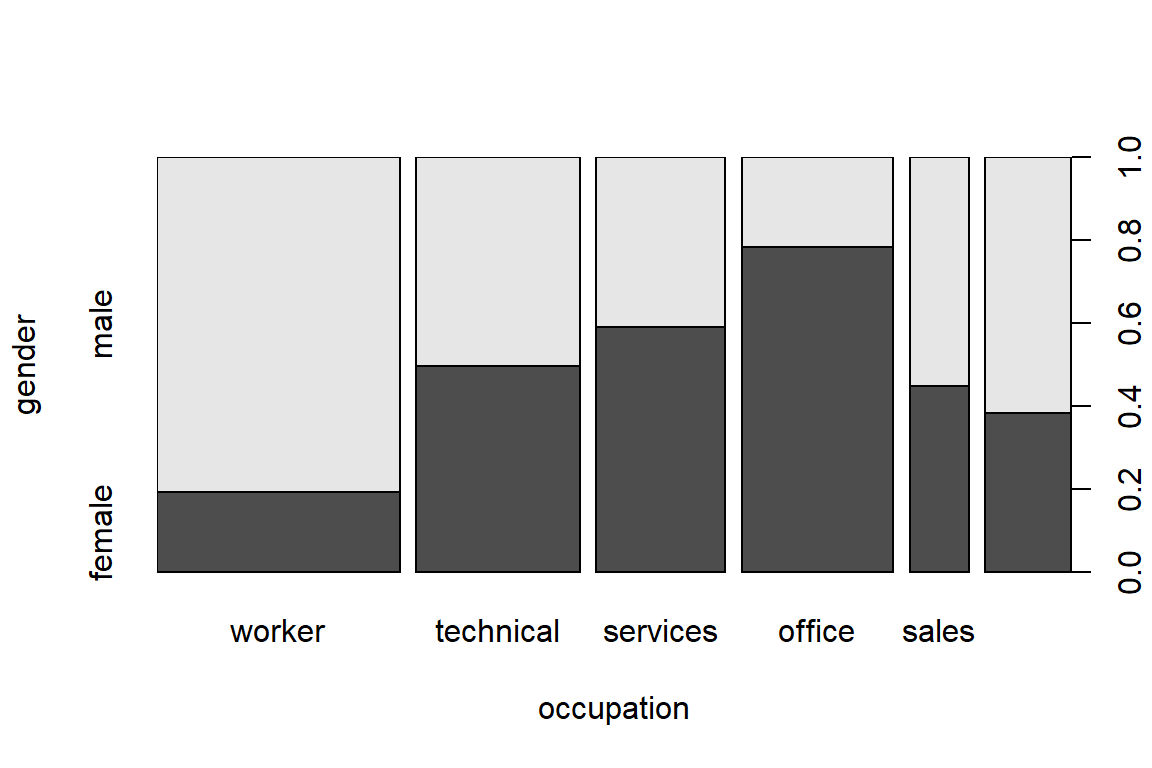
\includegraphics{_main_files/figure-latex/unnamed-chunk-114-1} \end{center}

\begin{center}\includegraphics{_main_files/figure-latex/unnamed-chunk-114-2} \end{center}

\begin{center}\includegraphics{_main_files/figure-latex/unnamed-chunk-114-3} \end{center}

\begin{center}\includegraphics{_main_files/figure-latex/unnamed-chunk-114-4} \end{center}

Or you can construct your own plots, e.g.~by adding the least squares line to the scatter plot.

\begin{Shaded}
\begin{Highlighting}[]
\CommentTok{# add the regression line to the scatter plot}
\KeywordTok{plot}\NormalTok{(car_price}\OperatorTok{$}\NormalTok{income, car_price}\OperatorTok{$}\NormalTok{price, }\DataTypeTok{pch=}\DecValTok{21}\NormalTok{, }\DataTypeTok{cex=}\FloatTok{1.2}\NormalTok{, }\DataTypeTok{xlab =} \StringTok{"income"}\NormalTok{, }\DataTypeTok{main =} \StringTok{"Simple linear regression"}\NormalTok{)}
\CommentTok{# add LS line like this}
\KeywordTok{abline}\NormalTok{(lm1, }\DataTypeTok{col=}\StringTok{"blue"}\NormalTok{, }\DataTypeTok{lwd=}\DecValTok{2}\NormalTok{)}
\CommentTok{# or like this}
\KeywordTok{abline}\NormalTok{(lm1}\OperatorTok{$}\NormalTok{coefficients[}\DecValTok{1}\NormalTok{], lm1}\OperatorTok{$}\NormalTok{coefficients[}\DecValTok{2}\NormalTok{])}
\end{Highlighting}
\end{Shaded}

\begin{center}\includegraphics{_main_files/figure-latex/unnamed-chunk-115-1} \end{center}

Similarly, you can illustrate the fit with \texttt{ggplot}.

\begin{Shaded}
\begin{Highlighting}[]
\KeywordTok{ggplot}\NormalTok{(car_price, }\KeywordTok{aes}\NormalTok{(}\DataTypeTok{x =}\NormalTok{ income, }\DataTypeTok{y =}\NormalTok{ price)) }\OperatorTok{+}\StringTok{ }
\StringTok{ }\KeywordTok{theme_bw}\NormalTok{() }\OperatorTok{+}
\StringTok{ }\KeywordTok{geom_point}\NormalTok{(}\DataTypeTok{shape=}\DecValTok{1}\NormalTok{, }\DataTypeTok{alpha =} \DecValTok{1}\OperatorTok{/}\DecValTok{2}\NormalTok{) }\OperatorTok{+}\StringTok{ }
\StringTok{ }\KeywordTok{geom_smooth}\NormalTok{()}\OperatorTok{+}\KeywordTok{geom_abline}\NormalTok{(}\DataTypeTok{intercept =}\NormalTok{ lm1}\OperatorTok{$}\NormalTok{coef[}\DecValTok{1}\NormalTok{], }\DataTypeTok{slope =}\NormalTok{ lm1}\OperatorTok{$}\NormalTok{coef[}\DecValTok{2}\NormalTok{],   }\DataTypeTok{colour=}\StringTok{"red"}\NormalTok{, }\DataTypeTok{size=}\FloatTok{1.25}\NormalTok{) }
\end{Highlighting}
\end{Shaded}

\begin{verbatim}
`geom_smooth()` using method = 'loess' and formula 'y ~ x'
\end{verbatim}

\begin{center}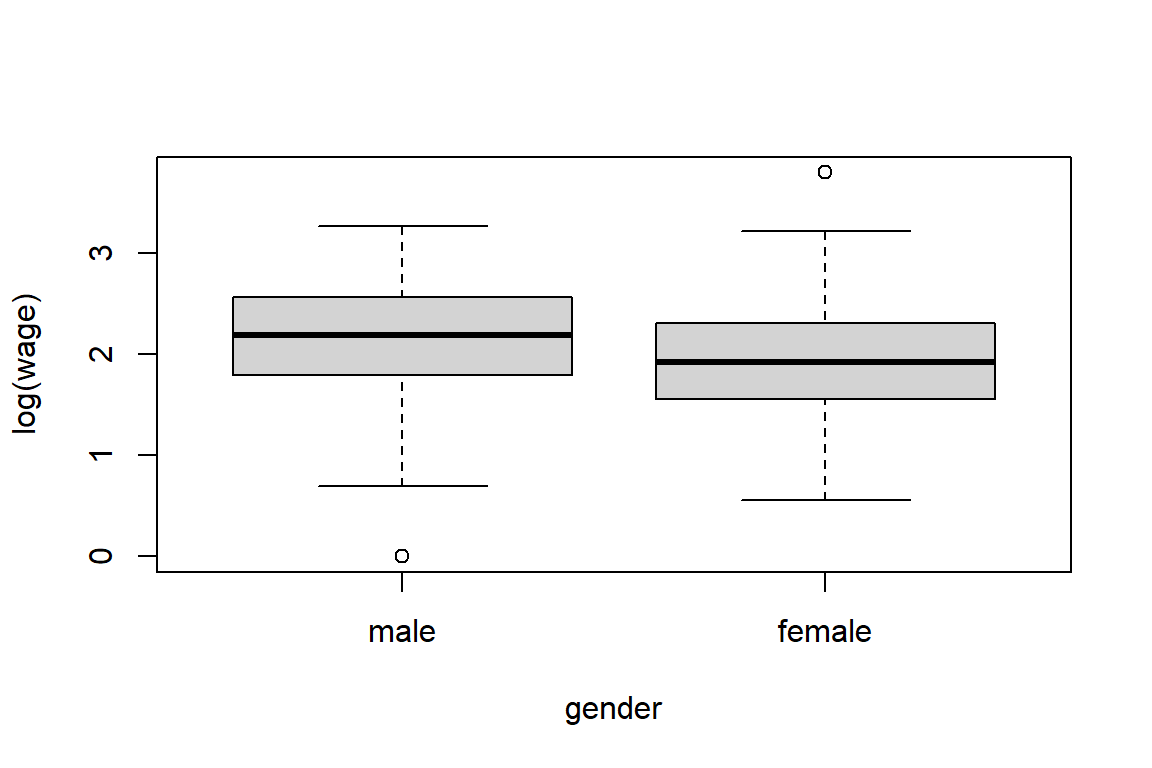
\includegraphics{_main_files/figure-latex/unnamed-chunk-116-1} \end{center}

The least squares fit minimizes the sum of the squares of the vertical distances between the observed response values and the least squares line (or plane). You now graphically illustrate what vertical distance means.

\begin{Shaded}
\begin{Highlighting}[]
\KeywordTok{plot}\NormalTok{(car_price}\OperatorTok{$}\NormalTok{income, car_price}\OperatorTok{$}\NormalTok{price, }\DataTypeTok{pch=}\DecValTok{21}\NormalTok{, }\DataTypeTok{cex=}\FloatTok{1.2}\NormalTok{, }\DataTypeTok{xlab =} \StringTok{"income"}\NormalTok{, }\DataTypeTok{main =} \StringTok{"Simple linear regression"}\NormalTok{)}
\KeywordTok{abline}\NormalTok{(lm1, }\DataTypeTok{col =} \StringTok{"blue"}\NormalTok{, }\DataTypeTok{lwd=}\DecValTok{2}\NormalTok{)}
\KeywordTok{segments}\NormalTok{(car_price}\OperatorTok{$}\NormalTok{income, car_price}\OperatorTok{$}\NormalTok{price, car_price}\OperatorTok{$}\NormalTok{income, lm1}\OperatorTok{$}\NormalTok{fitted.values, }\DataTypeTok{lty=}\DecValTok{1}\NormalTok{)}
\end{Highlighting}
\end{Shaded}

\begin{center}\includegraphics{_main_files/figure-latex/unnamed-chunk-117-1} \end{center}

You now return to the \texttt{summary(lm1)} and try to understand the (rest of the) output that is printed.

\begin{Shaded}
\begin{Highlighting}[]
\KeywordTok{summary}\NormalTok{(lm1)}
\end{Highlighting}
\end{Shaded}

\begin{verbatim}

Call:
lm(formula = price ~ income, data = car_price)

Residuals:
   Min     1Q Median     3Q    Max 
 -5365  -1185   -251   1334   6284 

Coefficients:
            Estimate Std. Error t value Pr(>|t|)    
(Intercept) 5.87e+03   7.50e+02    7.82  9.8e-11 ***
income      2.11e-01   1.51e-02   14.01  < 2e-16 ***
---
Signif. codes:  0 '***' 0.001 '**' 0.01 '*' 0.05 '.' 0.1 ' ' 1

Residual standard error: 2460 on 60 degrees of freedom
Multiple R-squared:  0.766,	Adjusted R-squared:  0.762 
F-statistic:  196 on 1 and 60 DF,  p-value: <2e-16
\end{verbatim}

Recall that in a general linear model \(Y = X\beta + \epsilon\) where \(E[\epsilon]=0\) and \(\text{Var}(\epsilon)=\sigma^2 I\) with \(I\) the identity matrix, the following estimator is used for the variance of the error terms
\begin{eqnarray*}
s^2 &=& \frac{1}{n-(p+1)}(Y-X\hat{\beta})^{'}(Y-X\hat{\beta}),
\end{eqnarray*}
where \(\beta = (\beta_0, \beta_1, \ldots, \beta_p)^{'}\).

You can recognize this in the output of \texttt{lm1} as follows

\begin{Shaded}
\begin{Highlighting}[]
\NormalTok{error.SS <-}\StringTok{ }\KeywordTok{sum}\NormalTok{(lm1}\OperatorTok{$}\NormalTok{resid}\OperatorTok{^}\DecValTok{2}\NormalTok{)}
\NormalTok{error.SS}
\end{Highlighting}
\end{Shaded}

\begin{verbatim}
[1] 362851718
\end{verbatim}

\begin{Shaded}
\begin{Highlighting}[]
\KeywordTok{sqrt}\NormalTok{(error.SS}\OperatorTok{/}\NormalTok{(}\KeywordTok{nrow}\NormalTok{(car_price)}\OperatorTok{-}\DecValTok{2}\NormalTok{))}
\end{Highlighting}
\end{Shaded}

\begin{verbatim}
[1] 2459.2
\end{verbatim}

The proportion of the variability in the data that is explained by the regression model is
\begin{eqnarray*}
R^2 &=& \frac{\text{Regression SS}}{\text{Total SS}} \\
&=& \frac{\sum_{i=1}^n (\hat{Y}_i-\bar{Y})^2}{\sum_{i=1}^n (Y_i-\bar{Y})^2} \\
&=& \frac{\sum_{i=1}^n (Y_i-\bar{Y})^2 - \sum_{i=1}^n (Y_i-\hat{Y})^2}{\sum_{i=1}^n (Y_i-\bar{Y})^2}.
\end{eqnarray*}

\begin{Shaded}
\begin{Highlighting}[]
\KeywordTok{attach}\NormalTok{(car_price)}
\NormalTok{total.SS <-}\StringTok{ }\KeywordTok{sum}\NormalTok{((price}\OperatorTok{-}\KeywordTok{mean}\NormalTok{(price))}\OperatorTok{^}\DecValTok{2}\NormalTok{)}
\NormalTok{total.SS}
\end{Highlighting}
\end{Shaded}

\begin{verbatim}
[1] 1549743871
\end{verbatim}

\begin{Shaded}
\begin{Highlighting}[]
\NormalTok{error.SS <-}\StringTok{ }\KeywordTok{sum}\NormalTok{(lm1}\OperatorTok{$}\NormalTok{resid}\OperatorTok{^}\DecValTok{2}\NormalTok{)}
\NormalTok{error.SS}
\end{Highlighting}
\end{Shaded}

\begin{verbatim}
[1] 362851718
\end{verbatim}

\begin{Shaded}
\begin{Highlighting}[]
\CommentTok{# R^2?}
\NormalTok{(total.SS}\OperatorTok{-}\NormalTok{error.SS)}\OperatorTok{/}\NormalTok{total.SS}
\end{Highlighting}
\end{Shaded}

\begin{verbatim}
[1] 0.76586
\end{verbatim}

\begin{Shaded}
\begin{Highlighting}[]
\KeywordTok{detach}\NormalTok{(car_price)}
\end{Highlighting}
\end{Shaded}

Finally, the output of \texttt{lm1} displays the result of a so-called \(F\) test, constructed as follows:

\begin{Shaded}
\begin{Highlighting}[]
\KeywordTok{attach}\NormalTok{(car_price)}
\CommentTok{# anova table in R?}
\KeywordTok{anova}\NormalTok{(lm1)}
\end{Highlighting}
\end{Shaded}

\begin{verbatim}
Analysis of Variance Table

Response: price
          Df   Sum Sq  Mean Sq F value Pr(>F)    
income     1 1.19e+09 1.19e+09     196 <2e-16 ***
Residuals 60 3.63e+08 6.05e+06                   
---
Signif. codes:  0 '***' 0.001 '**' 0.01 '*' 0.05 '.' 0.1 ' ' 1
\end{verbatim}

\begin{Shaded}
\begin{Highlighting}[]
\CommentTok{# F-statistic in anova and in output lm1?}
\NormalTok{lm0 <-}\StringTok{ }\KeywordTok{lm}\NormalTok{(price }\OperatorTok{~}\StringTok{ }\DecValTok{1}\NormalTok{)}
\NormalTok{error0.SS <-}\StringTok{ }\KeywordTok{sum}\NormalTok{(lm0}\OperatorTok{$}\NormalTok{resid}\OperatorTok{^}\DecValTok{2}\NormalTok{)}

\CommentTok{# calculate F-statistic}
\NormalTok{F <-}\StringTok{ }\NormalTok{((}\KeywordTok{anova}\NormalTok{(lm0)}\OperatorTok{$}\StringTok{"Sum Sq"}\NormalTok{)}\OperatorTok{-}\NormalTok{(}\KeywordTok{anova}\NormalTok{(lm1)}\OperatorTok{$}\StringTok{"Sum Sq"}\NormalTok{[}\DecValTok{2}\NormalTok{]))}\OperatorTok{/}\NormalTok{(}\KeywordTok{anova}\NormalTok{(lm1)}\OperatorTok{$}\StringTok{"Mean Sq"}\NormalTok{[}\DecValTok{2}\NormalTok{]) }
\NormalTok{F}
\end{Highlighting}
\end{Shaded}

\begin{verbatim}
[1] 196.26
\end{verbatim}

\begin{Shaded}
\begin{Highlighting}[]
\CommentTok{# critical values}
\KeywordTok{qf}\NormalTok{(}\FloatTok{0.95}\NormalTok{, }\DecValTok{1}\NormalTok{, }\DecValTok{60}\NormalTok{)}
\end{Highlighting}
\end{Shaded}

\begin{verbatim}
[1] 4.0012
\end{verbatim}

\begin{Shaded}
\begin{Highlighting}[]
\DecValTok{1}\OperatorTok{-}\KeywordTok{pf}\NormalTok{(F, }\DecValTok{1}\NormalTok{, }\DecValTok{60}\NormalTok{)}
\end{Highlighting}
\end{Shaded}

\begin{verbatim}
[1] 0
\end{verbatim}

\begin{Shaded}
\begin{Highlighting}[]
\KeywordTok{detach}\NormalTok{(car_price)}
\end{Highlighting}
\end{Shaded}

\begin{center}\rule{0.5\linewidth}{0.5pt}\end{center}

\hypertarget{a-multiple-linear-regression-model}{%
\section{A multiple linear regression model}\label{a-multiple-linear-regression-model}}

You'll now move on from simple to multiple linear regression. You model the
data by McDonald and Schwing (1973) published in Technometrics. The sampled data consists of variables obtained for year 1960 for 60 Standard Metropolitan
Statistical Areas (SMSA) in the US. The goal is to relate mortality in these SMSA to explanatory variables. For each sample area, you have information concerning the age-adjusted mortality rate for all causes, expressed as deaths per 100,000 population. This will be your response variable. The list of explanatory variables is:

\begin{itemize}
\tightlist
\item
  weather-related variables:
\item
  \texttt{prec}: average annual precipitation in inches
\item
  \texttt{jant}: average January temperature in degrees F
\item
  \texttt{jult}: average July temperature in degrees F
\item
  \texttt{humid}: annual average \% relative humidity at 1 pm
\item
  scocio-economic characteristics:
\item
  \texttt{ovr65}: \% of 1960 SMSA population aged 65 and older
\item
  \texttt{popn}: average household size
\item
  \texttt{educ} : median school years completed by those over 22
\item
  \texttt{hous} : \% of housing units which are sound and with all facilities
\item
  \texttt{educ} : median school years completed by those over 22
\item
  \texttt{dens} : population per sq mile in urbanized areas, 1960
\item
  \texttt{nonw} : \% of non-white population in urbanized areas, 1960
\item
  \texttt{wwdrk} : \% of employed in white collar occupations
\item
  \texttt{poor} : \% of families with income less than \$3,000
\item
  pollutants:
\item
  \texttt{hc} : relative pollution potential of hydrocarbons
\item
  \texttt{nox} : relative pollution potential of oxides of nitrogen
\item
  \texttt{so2}: relative pollution potential of sulfur dioxides
\end{itemize}

First, you'll load the data.

\begin{Shaded}
\begin{Highlighting}[]
\NormalTok{path <-}\StringTok{ }\KeywordTok{file.path}\NormalTok{(}\StringTok{'data'}\NormalTok{)}
\NormalTok{path.mort <-}\StringTok{ }\KeywordTok{file.path}\NormalTok{(path, }\StringTok{"pollution.csv"}\NormalTok{)}
\NormalTok{mort_poll <-}\StringTok{ }\KeywordTok{read.csv}\NormalTok{(path.mort)}
\end{Highlighting}
\end{Shaded}

Then, you'll explore the data.

\begin{Shaded}
\begin{Highlighting}[]
\KeywordTok{attach}\NormalTok{(mort_poll)}
\KeywordTok{summary}\NormalTok{(mort_poll)}
\end{Highlighting}
\end{Shaded}

\begin{verbatim}
      prec           jant           jult          ovr65            popn     
 Min.   :10.0   Min.   :12.0   Min.   :63.0   Min.   : 5.60   Min.   :2.92  
 1st Qu.:32.8   1st Qu.:27.0   1st Qu.:72.0   1st Qu.: 7.67   1st Qu.:3.21  
 Median :38.0   Median :31.5   Median :74.0   Median : 9.00   Median :3.27  
 Mean   :37.4   Mean   :34.0   Mean   :74.6   Mean   : 8.80   Mean   :3.26  
 3rd Qu.:43.2   3rd Qu.:40.0   3rd Qu.:77.2   3rd Qu.: 9.70   3rd Qu.:3.36  
 Max.   :60.0   Max.   :67.0   Max.   :85.0   Max.   :11.80   Max.   :3.53  
      educ           hous           dens           nonw           wwdrk     
 Min.   : 9.0   Min.   :66.8   Min.   :1441   Min.   : 0.80   Min.   :33.8  
 1st Qu.:10.4   1st Qu.:78.4   1st Qu.:3104   1st Qu.: 4.95   1st Qu.:43.2  
 Median :11.1   Median :81.2   Median :3567   Median :10.40   Median :45.5  
 Mean   :11.0   Mean   :80.9   Mean   :3876   Mean   :11.87   Mean   :46.1  
 3rd Qu.:11.5   3rd Qu.:83.6   3rd Qu.:4520   3rd Qu.:15.65   3rd Qu.:49.5  
 Max.   :12.3   Max.   :90.7   Max.   :9699   Max.   :38.50   Max.   :59.7  
      poor            hc             nox             so2            humid     
 Min.   : 9.4   Min.   :  1.0   Min.   :  1.0   Min.   :  1.0   Min.   :38.0  
 1st Qu.:12.0   1st Qu.:  7.0   1st Qu.:  4.0   1st Qu.: 11.0   1st Qu.:55.0  
 Median :13.2   Median : 14.5   Median :  9.0   Median : 30.0   Median :57.0  
 Mean   :14.4   Mean   : 37.9   Mean   : 22.6   Mean   : 53.8   Mean   :57.7  
 3rd Qu.:15.2   3rd Qu.: 30.2   3rd Qu.: 23.8   3rd Qu.: 69.0   3rd Qu.:60.0  
 Max.   :26.4   Max.   :648.0   Max.   :319.0   Max.   :278.0   Max.   :73.0  
      mort     
 Min.   : 791  
 1st Qu.: 898  
 Median : 944  
 Mean   : 940  
 3rd Qu.: 983  
 Max.   :1113  
\end{verbatim}

\begin{Shaded}
\begin{Highlighting}[]
\CommentTok{# get correlation matrix}
\KeywordTok{round}\NormalTok{(}\KeywordTok{cor}\NormalTok{(mort_poll), }\DecValTok{4}\NormalTok{)}
\end{Highlighting}
\end{Shaded}

\begin{verbatim}
         prec    jant    jult   ovr65    popn    educ    hous    dens    nonw
prec   1.0000  0.0922  0.5033  0.1011  0.2634 -0.4904 -0.4908 -0.0035  0.4132
jant   0.0922  1.0000  0.3463 -0.3981 -0.2092  0.1163  0.0149 -0.1001  0.4538
jult   0.5033  0.3463  1.0000 -0.4340  0.2623 -0.2385 -0.4150 -0.0610  0.5753
ovr65  0.1011 -0.3981 -0.4340  1.0000 -0.5091 -0.1389  0.0650  0.1620 -0.6378
popn   0.2634 -0.2092  0.2623 -0.5091  1.0000 -0.3951 -0.4106 -0.1843  0.4194
educ  -0.4904  0.1163 -0.2385 -0.1389 -0.3951  1.0000  0.5522 -0.2439 -0.2088
hous  -0.4908  0.0149 -0.4150  0.0650 -0.4106  0.5522  1.0000  0.1819 -0.4103
dens  -0.0035 -0.1001 -0.0610  0.1620 -0.1843 -0.2439  0.1819  1.0000 -0.0057
nonw   0.4132  0.4538  0.5753 -0.6378  0.4194 -0.2088 -0.4103 -0.0057  1.0000
wwdrk -0.2973  0.2380 -0.0214 -0.1177 -0.4257  0.7032  0.3387 -0.0318 -0.0044
poor   0.5066  0.5653  0.6193 -0.3098  0.2599 -0.4033 -0.6807 -0.1629  0.7049
hc    -0.5318  0.3508 -0.3565 -0.0205 -0.3882  0.2868  0.3868  0.1203 -0.0259
nox   -0.4873  0.3210 -0.3377 -0.0021 -0.3584  0.2244  0.3483  0.1653  0.0184
so2   -0.1069 -0.1078 -0.0993  0.0172 -0.0041 -0.2343  0.1180  0.4321  0.1593
humid -0.0773  0.0679 -0.4528  0.1124 -0.1357  0.1765  0.1219 -0.1250 -0.1180
mort   0.5095 -0.0300  0.2770 -0.1746  0.3573 -0.5110 -0.4268  0.2655  0.6437
        wwdrk    poor      hc     nox     so2   humid    mort
prec  -0.2973  0.5066 -0.5318 -0.4873 -0.1069 -0.0773  0.5095
jant   0.2380  0.5653  0.3508  0.3210 -0.1078  0.0679 -0.0300
jult  -0.0214  0.6193 -0.3565 -0.3377 -0.0993 -0.4528  0.2770
ovr65 -0.1177 -0.3098 -0.0205 -0.0021  0.0172  0.1124 -0.1746
popn  -0.4257  0.2599 -0.3882 -0.3584 -0.0041 -0.1357  0.3573
educ   0.7032 -0.4033  0.2868  0.2244 -0.2343  0.1765 -0.5110
hous   0.3387 -0.6807  0.3868  0.3483  0.1180  0.1219 -0.4268
dens  -0.0318 -0.1629  0.1203  0.1653  0.4321 -0.1250  0.2655
nonw  -0.0044  0.7049 -0.0259  0.0184  0.1593 -0.1180  0.6437
wwdrk  1.0000 -0.1852  0.2037  0.1600 -0.0685  0.0607 -0.2848
poor  -0.1852  1.0000 -0.1298 -0.1025 -0.0965 -0.1522  0.4105
hc     0.2037 -0.1298  1.0000  0.9838  0.2823 -0.0202 -0.1772
nox    0.1600 -0.1025  0.9838  1.0000  0.4094 -0.0459 -0.0774
so2   -0.0685 -0.0965  0.2823  0.4094  1.0000 -0.1026  0.4259
humid  0.0607 -0.1522 -0.0202 -0.0459 -0.1026  1.0000 -0.0885
mort  -0.2848  0.4105 -0.1772 -0.0774  0.4259 -0.0885  1.0000
\end{verbatim}

\begin{Shaded}
\begin{Highlighting}[]
\CommentTok{# create dataframes}
\CommentTok{# weather related vars}
\NormalTok{mort_poll_}\DecValTok{1}\NormalTok{ <-}\StringTok{ }\KeywordTok{data.frame}\NormalTok{(mort, prec, jant, jult, humid)}
\CommentTok{# socio-economic vars}
\NormalTok{mort_poll_}\DecValTok{2}\NormalTok{ <-}\StringTok{ }\KeywordTok{data.frame}\NormalTok{(mort, ovr65, popn, educ, hous, dens, nonw, wwdrk, poor)}
\CommentTok{# pollution effects}
\NormalTok{mort_poll_}\DecValTok{3}\NormalTok{ <-}\StringTok{ }\KeywordTok{data.frame}\NormalTok{(mort, hc, nox, so2)}

\CommentTok{# matrix scatterplots}
\KeywordTok{pairs}\NormalTok{(mort_poll_}\DecValTok{1}\NormalTok{, }\DataTypeTok{cex=}\DecValTok{1}\NormalTok{, }\DataTypeTok{pch=}\DecValTok{19}\NormalTok{)}
\end{Highlighting}
\end{Shaded}

\begin{center}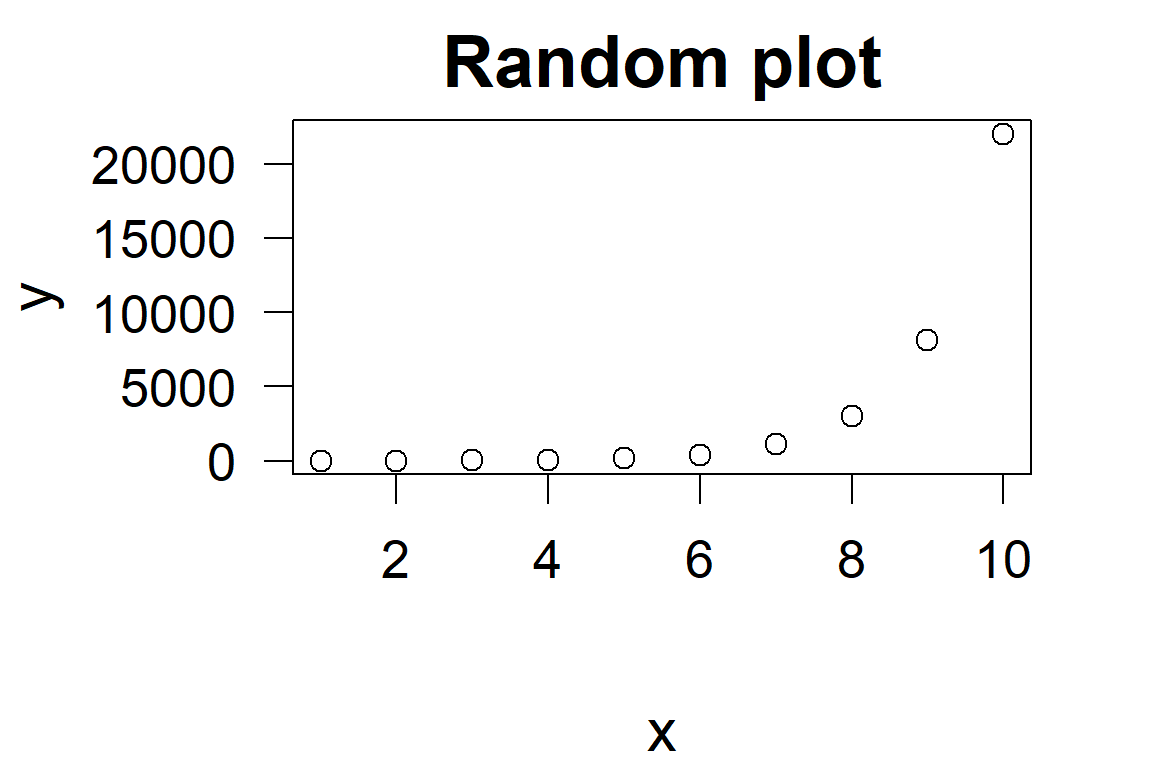
\includegraphics{_main_files/figure-latex/unnamed-chunk-123-1} \end{center}

\begin{Shaded}
\begin{Highlighting}[]
\KeywordTok{pairs}\NormalTok{(mort_poll_}\DecValTok{2}\NormalTok{, }\DataTypeTok{cex=}\FloatTok{0.5}\NormalTok{, }\DataTypeTok{pch=}\DecValTok{19}\NormalTok{)}
\end{Highlighting}
\end{Shaded}

\begin{center}\includegraphics{_main_files/figure-latex/unnamed-chunk-123-2} \end{center}

\begin{Shaded}
\begin{Highlighting}[]
\KeywordTok{pairs}\NormalTok{(mort_poll_}\DecValTok{3}\NormalTok{, }\DataTypeTok{cex=}\DecValTok{1}\NormalTok{, }\DataTypeTok{pch=}\DecValTok{19}\NormalTok{)}
\end{Highlighting}
\end{Shaded}

\begin{center}\includegraphics{_main_files/figure-latex/unnamed-chunk-123-3} \end{center}

\begin{Shaded}
\begin{Highlighting}[]
\KeywordTok{detach}\NormalTok{(mort_poll)}
\end{Highlighting}
\end{Shaded}

First, you fit a rather simple linear model to explain \texttt{mort}. That is
\begin{eqnarray*}
Y &=& \beta_0 + \beta_1 x_{i1} + \beta_2 x_{i2} + \epsilon_i,
\end{eqnarray*}
where \(\beta_0\) is the intercept, \(x_1\) the \texttt{educ} and \(x_2\) the \texttt{so2}.

\begin{Shaded}
\begin{Highlighting}[]
\KeywordTok{attach}\NormalTok{(mort_poll)}
\NormalTok{lm1 <-}\StringTok{ }\KeywordTok{lm}\NormalTok{(mort }\OperatorTok{~}\StringTok{ }\NormalTok{educ }\OperatorTok{+}\StringTok{ }\NormalTok{so2)}
\KeywordTok{summary}\NormalTok{(lm1)}
\end{Highlighting}
\end{Shaded}

\begin{verbatim}

Call:
lm(formula = mort ~ educ + so2)

Residuals:
    Min      1Q  Median      3Q     Max 
-136.56  -30.37   -7.73   34.48  148.80 

Coefficients:
            Estimate Std. Error t value Pr(>|t|)    
(Intercept) 1274.602     89.761   14.20  < 2e-16 ***
educ         -32.017      8.020   -3.99  0.00019 ***
so2            0.318      0.107    2.97  0.00432 ** 
---
Signif. codes:  0 '***' 0.001 '**' 0.01 '*' 0.05 '.' 0.1 ' ' 1

Residual standard error: 50.6 on 57 degrees of freedom
Multiple R-squared:  0.36,	Adjusted R-squared:  0.338 
F-statistic: 16.1 on 2 and 57 DF,  p-value: 2.96e-06
\end{verbatim}

\begin{Shaded}
\begin{Highlighting}[]
\KeywordTok{detach}\NormalTok{(mort_poll)}
\end{Highlighting}
\end{Shaded}

You inspect the analysis-of-variance table for this linear model \texttt{lm1}. That is

\begin{Shaded}
\begin{Highlighting}[]
\KeywordTok{anova}\NormalTok{(lm1)}
\end{Highlighting}
\end{Shaded}

\begin{verbatim}
Analysis of Variance Table

Response: mort
          Df Sum Sq Mean Sq F value  Pr(>F)    
educ       1  59612   59612   23.26 1.1e-05 ***
so2        1  22642   22642    8.84  0.0043 ** 
Residuals 57 146054    2562                    
---
Signif. codes:  0 '***' 0.001 '**' 0.01 '*' 0.05 '.' 0.1 ' ' 1
\end{verbatim}

\begin{Shaded}
\begin{Highlighting}[]
\KeywordTok{attach}\NormalTok{(mort_poll)}
\NormalTok{lm0 <-}\StringTok{ }\KeywordTok{lm}\NormalTok{(mort }\OperatorTok{~}\StringTok{ }\DecValTok{1}\NormalTok{)}
\NormalTok{lm_educ <-}\StringTok{ }\KeywordTok{lm}\NormalTok{(mort }\OperatorTok{~}\StringTok{ }\NormalTok{educ)}
\KeywordTok{anova}\NormalTok{(lm_educ)}
\end{Highlighting}
\end{Shaded}

\begin{verbatim}
Analysis of Variance Table

Response: mort
          Df Sum Sq Mean Sq F value Pr(>F)    
educ       1  59612   59612    20.5  3e-05 ***
Residuals 58 168696    2909                   
---
Signif. codes:  0 '***' 0.001 '**' 0.01 '*' 0.05 '.' 0.1 ' ' 1
\end{verbatim}

\begin{Shaded}
\begin{Highlighting}[]
\NormalTok{F_educ <-}\StringTok{ }\NormalTok{((}\KeywordTok{anova}\NormalTok{(lm0)}\OperatorTok{$}\StringTok{"Sum Sq"}\NormalTok{)}\OperatorTok{-}\NormalTok{(}\KeywordTok{anova}\NormalTok{(lm_educ)}\OperatorTok{$}\StringTok{"Sum Sq"}\NormalTok{[}\DecValTok{2}\NormalTok{]))}\OperatorTok{/}\NormalTok{(}\KeywordTok{anova}\NormalTok{(lm1)}\OperatorTok{$}\StringTok{"Mean Sq"}\NormalTok{[}\DecValTok{3}\NormalTok{]) }
\NormalTok{F_educ}
\end{Highlighting}
\end{Shaded}

\begin{verbatim}
[1] 23.265
\end{verbatim}

\begin{Shaded}
\begin{Highlighting}[]
\NormalTok{F_so2 <-}\StringTok{ }\NormalTok{((}\KeywordTok{anova}\NormalTok{(lm_educ)}\OperatorTok{$}\StringTok{"Sum Sq"}\NormalTok{[}\DecValTok{2}\NormalTok{])}\OperatorTok{-}\NormalTok{(}\KeywordTok{anova}\NormalTok{(lm1)}\OperatorTok{$}\StringTok{"Sum Sq"}\NormalTok{[}\DecValTok{3}\NormalTok{]))}\OperatorTok{/}\NormalTok{(}\KeywordTok{anova}\NormalTok{(lm1)}\OperatorTok{$}\StringTok{"Mean Sq"}\NormalTok{[}\DecValTok{3}\NormalTok{]) }
\NormalTok{F_so2}
\end{Highlighting}
\end{Shaded}

\begin{verbatim}
[1] 8.8363
\end{verbatim}

\begin{Shaded}
\begin{Highlighting}[]
\KeywordTok{detach}\NormalTok{(mort_poll)}
\end{Highlighting}
\end{Shaded}

You will now use the object \texttt{lm1} to construct confidence and prediction intervals for a single observation. Given a set of predictor values in \(x_0\) the predicted response is \(\hat{y}_0 = x_0^{'}\hat{\beta}\). The uncertainty in predicting the mean response is \(\text{Var}(x_0^{'}\hat{\beta})\) whereas the uncertainty in predicting the value of an observation is \(\text{Var}(x_0^{'}\hat{\beta}+\epsilon_0)\).

\begin{Shaded}
\begin{Highlighting}[]
\KeywordTok{attach}\NormalTok{(mort_poll)}
\NormalTok{x0 <-}\StringTok{ }\KeywordTok{data.frame}\NormalTok{(}\DataTypeTok{educ =} \DecValTok{10}\NormalTok{, }\DataTypeTok{so2 =} \KeywordTok{exp}\NormalTok{(}\DecValTok{2}\NormalTok{))}
\KeywordTok{predict}\NormalTok{(lm1, x0, }\DataTypeTok{interval =} \StringTok{"confidence"}\NormalTok{)}
\end{Highlighting}
\end{Shaded}

\begin{verbatim}
     fit    lwr    upr
1 956.78 932.55 981.01
\end{verbatim}

\begin{Shaded}
\begin{Highlighting}[]
\KeywordTok{predict}\NormalTok{(lm1, x0, }\DataTypeTok{interval =} \StringTok{"prediction"}\NormalTok{)}
\end{Highlighting}
\end{Shaded}

\begin{verbatim}
     fit    lwr  upr
1 956.78 852.56 1061
\end{verbatim}

\begin{Shaded}
\begin{Highlighting}[]
\KeywordTok{detach}\NormalTok{(mort_poll)}
\end{Highlighting}
\end{Shaded}

For a grid of \texttt{educ} values, when \texttt{so2} is fixed, this goes as follows:

\begin{Shaded}
\begin{Highlighting}[]
\KeywordTok{attach}\NormalTok{(mort_poll)}
\NormalTok{grid <-}\StringTok{ }\KeywordTok{seq}\NormalTok{(}\DecValTok{8}\NormalTok{, }\DecValTok{15}\NormalTok{, }\FloatTok{0.1}\NormalTok{)}
\NormalTok{x.new <-}\StringTok{ }\KeywordTok{data.frame}\NormalTok{(}\DataTypeTok{educ =}\NormalTok{ grid, }\DataTypeTok{so2 =} \KeywordTok{exp}\NormalTok{(}\DecValTok{2}\NormalTok{))}
\NormalTok{p <-}\StringTok{ }\KeywordTok{predict}\NormalTok{(lm1, x.new, }\DataTypeTok{se=}\OtherTok{TRUE}\NormalTok{, }\DataTypeTok{interval=}\StringTok{"prediction"}\NormalTok{)}
\NormalTok{p1 <-}\StringTok{ }\KeywordTok{predict}\NormalTok{(lm1, x.new, }\DataTypeTok{se=}\OtherTok{TRUE}\NormalTok{, }\DataTypeTok{interval=}\StringTok{"confidence"}\NormalTok{)}
\CommentTok{# use `matplot` to plot the columns of one matrix against the columnsof another}
\KeywordTok{matplot}\NormalTok{(grid, p}\OperatorTok{$}\NormalTok{fit, }\DataTypeTok{lty=}\KeywordTok{c}\NormalTok{(}\DecValTok{1}\NormalTok{,}\DecValTok{2}\NormalTok{,}\DecValTok{2}\NormalTok{), }\DataTypeTok{col=}\KeywordTok{c}\NormalTok{(}\StringTok{"black"}\NormalTok{, }\StringTok{"red"}\NormalTok{, }\StringTok{"red"}\NormalTok{), }\DataTypeTok{type =} \StringTok{"l"}\NormalTok{, }\DataTypeTok{xlab =} \StringTok{"educ"}\NormalTok{, }\DataTypeTok{ylab =} \StringTok{"mort"}\NormalTok{, }\DataTypeTok{main =} \StringTok{"Predicted mort over a range of educ, log(so2)=2"}\NormalTok{)}
\KeywordTok{matlines}\NormalTok{(grid, p1}\OperatorTok{$}\NormalTok{fit, }\DataTypeTok{lty =} \KeywordTok{c}\NormalTok{(}\DecValTok{1}\NormalTok{, }\DecValTok{2}\NormalTok{, }\DecValTok{2}\NormalTok{), }\DataTypeTok{col =} \KeywordTok{c}\NormalTok{(}\StringTok{"black"}\NormalTok{, }\StringTok{"blue"}\NormalTok{, }\StringTok{"blue"}\NormalTok{))}
\KeywordTok{rug}\NormalTok{(educ)}
\end{Highlighting}
\end{Shaded}

\begin{center}\includegraphics{_main_files/figure-latex/unnamed-chunk-127-1} \end{center}

\begin{Shaded}
\begin{Highlighting}[]
\CommentTok{# for an explanation wrt different shapes, see }
\CommentTok{# http://stats.stackexchange.com/questions/85560/shape-of-confidence-interval-for-p# redicted-values-in-linear-regression}
\KeywordTok{detach}\NormalTok{(mort_poll)}
\end{Highlighting}
\end{Shaded}

Then you fit a linear model with all 15 variables in the dataset.

\begin{Shaded}
\begin{Highlighting}[]
\KeywordTok{attach}\NormalTok{(mort_poll)}
\NormalTok{lm2 <-}\StringTok{ }\KeywordTok{lm}\NormalTok{(mort }\OperatorTok{~}\StringTok{ }\NormalTok{prec }\OperatorTok{+}\StringTok{ }\NormalTok{jant }\OperatorTok{+}\StringTok{ }\NormalTok{jult }\OperatorTok{+}\StringTok{ }\NormalTok{humid }\OperatorTok{+}\StringTok{ }\NormalTok{hc }\OperatorTok{+}\StringTok{ }\NormalTok{nox }\OperatorTok{+}\StringTok{ }\NormalTok{so2 }\OperatorTok{+}\StringTok{ }\NormalTok{ovr65 }\OperatorTok{+}\StringTok{ }\NormalTok{popn }\OperatorTok{+}\StringTok{ }\NormalTok{educ }\OperatorTok{+}\StringTok{ }\NormalTok{hous }\OperatorTok{+}\StringTok{ }\NormalTok{dens }\OperatorTok{+}\StringTok{ }\NormalTok{nonw }\OperatorTok{+}\StringTok{ }\NormalTok{wwdrk }\OperatorTok{+}\StringTok{ }\NormalTok{poor)}
\NormalTok{lm2}\OperatorTok{$}\NormalTok{coef}
\end{Highlighting}
\end{Shaded}

\begin{verbatim}
(Intercept)        prec        jant        jult       humid          hc 
 1.7640e+03  1.9054e+00 -1.9376e+00 -3.1004e+00  1.0680e-01 -6.7214e-01 
        nox         so2       ovr65        popn        educ        hous 
 1.3401e+00  8.6252e-02 -9.0654e+00 -1.0683e+02 -1.7157e+01 -6.5112e-01 
       dens        nonw       wwdrk        poor 
 3.6005e-03  4.4596e+00 -1.8706e-01 -1.6764e-01 
\end{verbatim}

\begin{Shaded}
\begin{Highlighting}[]
\KeywordTok{detach}\NormalTok{(mort_poll)}
\end{Highlighting}
\end{Shaded}

Now perform model selection stepwise, based on AIC.

\begin{Shaded}
\begin{Highlighting}[]
\CommentTok{# model selection based on AIC}
\KeywordTok{library}\NormalTok{(MASS)}
\end{Highlighting}
\end{Shaded}

\begin{verbatim}

Attaching package: 'MASS'
\end{verbatim}

\begin{verbatim}
The following object is masked from 'package:dplyr':

    select
\end{verbatim}

\begin{Shaded}
\begin{Highlighting}[]
\KeywordTok{attach}\NormalTok{(mort_poll)}
\NormalTok{lm1 <-}\StringTok{ }\KeywordTok{lm}\NormalTok{(mort }\OperatorTok{~}\StringTok{ }\DecValTok{1}\NormalTok{)}
\CommentTok{# get AIC, mind the difference}
\KeywordTok{AIC}\NormalTok{(lm1)}
\end{Highlighting}
\end{Shaded}

\begin{verbatim}
[1] 668.92
\end{verbatim}

\begin{Shaded}
\begin{Highlighting}[]
\KeywordTok{extractAIC}\NormalTok{(lm1)}
\end{Highlighting}
\end{Shaded}

\begin{verbatim}
[1]   1.00 496.65
\end{verbatim}

\begin{Shaded}
\begin{Highlighting}[]
\CommentTok{# for linear models with unknown scale (i.e., for lm and aov), }
\CommentTok{# -2 log L is computed from the deviance and uses a different additive constant to }
\CommentTok{# logLik and hence AIC }

\CommentTok{# forward search}
\KeywordTok{stepAIC}\NormalTok{(lm1, }\KeywordTok{list}\NormalTok{(}\DataTypeTok{upper =} \OperatorTok{~}\StringTok{ }\NormalTok{prec }\OperatorTok{+}\StringTok{ }\NormalTok{jant }\OperatorTok{+}\StringTok{ }\NormalTok{jult }\OperatorTok{+}\StringTok{ }\NormalTok{ovr65 }\OperatorTok{+}\StringTok{ }\NormalTok{popn }\OperatorTok{+}\StringTok{ }\NormalTok{educ }\OperatorTok{+}\StringTok{ }\NormalTok{hous }\OperatorTok{+}\StringTok{ }\NormalTok{dens }\OperatorTok{+}\StringTok{ }\NormalTok{nonw }\OperatorTok{+}\StringTok{ }\NormalTok{wwdrk }\OperatorTok{+}\StringTok{ }\NormalTok{poor }\OperatorTok{+}\StringTok{ }\NormalTok{hc }\OperatorTok{+}\StringTok{ }\KeywordTok{log}\NormalTok{(nox) }\OperatorTok{+}\StringTok{ }\KeywordTok{log}\NormalTok{(so2) }\OperatorTok{+}\StringTok{ }\NormalTok{humid, }\DataTypeTok{lower =} \OperatorTok{~}\StringTok{ }\DecValTok{1}\NormalTok{), }\DataTypeTok{direction =} \StringTok{"forward"}\NormalTok{)}
\end{Highlighting}
\end{Shaded}

\begin{verbatim}
Start:  AIC=496.65
mort ~ 1

           Df Sum of Sq    RSS AIC
+ nonw      1     94613 133695 467
+ educ      1     59612 168696 480
+ prec      1     59266 169041 481
+ hous      1     41592 186716 487
+ poor      1     38470 189838 488
+ log(so2)  1     37087 191221 488
+ popn      1     29149 199159 490
+ log(nox)  1     19465 208843 493
+ wwdrk     1     18518 209789 494
+ jult      1     17520 210788 494
+ dens      1     16093 212214 494
<none>                  228308 497
+ hc        1      7172 221136 497
+ ovr65     1      6960 221347 497
+ humid     1      1788 226520 498
+ jant      1       206 228102 499

Step:  AIC=466.54
mort ~ nonw

           Df Sum of Sq    RSS AIC
+ educ      1     33853  99841 451
+ log(so2)  1     31223 102471 453
+ jant      1     29835 103859 453
+ ovr65     1     21435 112259 458
+ wwdrk     1     18153 115541 460
+ dens      1     16540 117155 461
+ prec      1     16324 117371 461
+ hous      1      7264 126430 465
+ log(nox)  1      6836 126859 465
+ hc        1      5892 127803 466
<none>                  133695 467
+ jult      1      2973 130721 467
+ popn      1      2112 131582 468
+ poor      1       851 132844 468
+ humid     1        37 133658 469

Step:  AIC=451.02
mort ~ nonw + educ

           Df Sum of Sq   RSS AIC
+ log(so2)  1     18177 81664 441
+ jant      1     17453 82389 441
+ poor      1     10921 88920 446
+ log(nox)  1      8814 91027 447
+ ovr65     1      7352 92489 448
+ dens      1      7262 92579 448
+ jult      1      6836 93005 449
<none>                  99841 451
+ prec      1      2468 97373 452
+ hc        1       617 99224 453
+ humid     1       530 99312 453
+ popn      1       359 99482 453
+ hous      1       167 99674 453
+ wwdrk     1        14 99827 453

Step:  AIC=440.96
mort ~ nonw + educ + log(so2)

           Df Sum of Sq   RSS AIC
+ prec      1      9399 72266 436
+ jant      1      7885 73780 437
+ hc        1      6355 75309 438
+ ovr65     1      2770 78895 441
<none>                  81664 441
+ poor      1      2236 79428 441
+ dens      1       794 80871 442
+ humid     1       692 80973 442
+ hous      1       538 81126 443
+ log(nox)  1       312 81352 443
+ wwdrk     1       281 81383 443
+ jult      1       132 81532 443
+ popn      1         3 81661 443

Step:  AIC=435.63
mort ~ nonw + educ + log(so2) + prec

           Df Sum of Sq   RSS AIC
+ jant      1      5764 66502 433
+ poor      1      2878 69388 435
<none>                  72266 436
+ hc        1      1594 70672 436
+ log(nox)  1      1089 71177 437
+ jult      1       981 71285 437
+ dens      1       752 71513 437
+ humid     1       508 71758 437
+ wwdrk     1       405 71861 437
+ hous      1       125 72141 438
+ popn      1        70 72196 438
+ ovr65     1         2 72263 438

Step:  AIC=432.64
mort ~ nonw + educ + log(so2) + prec + jant

           Df Sum of Sq   RSS AIC
+ log(nox)  1      8313 58188 427
<none>                  66502 433
+ popn      1      1724 64778 433
+ dens      1      1455 65047 433
+ jult      1      1097 65405 434
+ humid     1       958 65544 434
+ poor      1       474 66028 434
+ hous      1        74 66428 435
+ ovr65     1        56 66446 435
+ wwdrk     1        27 66475 435
+ hc        1        25 66477 435

Step:  AIC=426.63
mort ~ nonw + educ + log(so2) + prec + jant + log(nox)

        Df Sum of Sq   RSS AIC
+ popn   1      2793 55396 426
<none>               58188 427
+ dens   1      1379 56810 427
+ hc     1       792 57396 428
+ jult   1        43 58145 429
+ poor   1        25 58164 429
+ humid  1        16 58172 429
+ hous   1         8 58181 429
+ wwdrk  1         6 58182 429
+ ovr65  1         0 58188 429

Step:  AIC=425.67
mort ~ nonw + educ + log(so2) + prec + jant + log(nox) + popn

        Df Sum of Sq   RSS AIC
<none>               55396 426
+ ovr65  1      1802 53594 426
+ hc     1      1587 53809 426
+ dens   1       570 54826 427
+ jult   1       142 55254 428
+ wwdrk  1       129 55267 428
+ poor   1        54 55341 428
+ humid  1        10 55386 428
+ hous   1         4 55392 428
\end{verbatim}

\begin{verbatim}

Call:
lm(formula = mort ~ nonw + educ + log(so2) + prec + jant + log(nox) + 
    popn)

Coefficients:
(Intercept)         nonw         educ     log(so2)         prec         jant  
    1315.91         4.50       -19.04        -6.15         2.19        -2.86  
   log(nox)         popn  
      24.01       -73.76  
\end{verbatim}

\begin{Shaded}
\begin{Highlighting}[]
\CommentTok{# backward search}
\NormalTok{lm1 <-}\StringTok{ }\KeywordTok{lm}\NormalTok{(mort }\OperatorTok{~}\StringTok{ }\NormalTok{prec }\OperatorTok{+}\StringTok{ }\NormalTok{jant }\OperatorTok{+}\StringTok{ }\NormalTok{jult }\OperatorTok{+}\StringTok{ }\NormalTok{ovr65 }\OperatorTok{+}\StringTok{ }\NormalTok{popn }\OperatorTok{+}\StringTok{ }\NormalTok{educ }\OperatorTok{+}\StringTok{ }\NormalTok{hous }\OperatorTok{+}\StringTok{ }\NormalTok{dens }\OperatorTok{+}\StringTok{ }\NormalTok{nonw }\OperatorTok{+}
\NormalTok{		 wwdrk }\OperatorTok{+}\StringTok{ }\NormalTok{poor }\OperatorTok{+}\StringTok{ }\NormalTok{hc }\OperatorTok{+}\StringTok{ }\KeywordTok{log}\NormalTok{(nox) }\OperatorTok{+}\StringTok{ }\KeywordTok{log}\NormalTok{(so2) }\OperatorTok{+}\StringTok{ }\NormalTok{humid)}
\KeywordTok{stepAIC}\NormalTok{(lm1, }\KeywordTok{list}\NormalTok{(}\DataTypeTok{upper =} \OperatorTok{~}\StringTok{ }\NormalTok{prec }\OperatorTok{+}\StringTok{ }\NormalTok{jant }\OperatorTok{+}\StringTok{ }\NormalTok{jult }\OperatorTok{+}\StringTok{ }\NormalTok{ovr65 }\OperatorTok{+}\StringTok{ }\NormalTok{popn }\OperatorTok{+}\StringTok{ }\NormalTok{educ }\OperatorTok{+}\StringTok{ }\NormalTok{hous }\OperatorTok{+}\StringTok{ }\NormalTok{dens }\OperatorTok{+}\StringTok{ }\NormalTok{nonw }\OperatorTok{+}\StringTok{ }\NormalTok{wwdrk }\OperatorTok{+}\StringTok{ }\NormalTok{poor }\OperatorTok{+}\StringTok{ }\NormalTok{hc }\OperatorTok{+}\StringTok{ }\KeywordTok{log}\NormalTok{(nox) }\OperatorTok{+}\StringTok{ }\KeywordTok{log}\NormalTok{(so2) }\OperatorTok{+}\StringTok{ }\NormalTok{humid, }\DataTypeTok{lower =} \OperatorTok{~}\StringTok{ }\DecValTok{1}\NormalTok{), }\DataTypeTok{direction =} \StringTok{"backward"}\NormalTok{)}
\end{Highlighting}
\end{Shaded}

\begin{verbatim}
Start:  AIC=435.55
mort ~ prec + jant + jult + ovr65 + popn + educ + hous + dens + 
    nonw + wwdrk + poor + hc + log(nox) + log(so2) + humid

           Df Sum of Sq   RSS AIC
- poor      1         1 50019 434
- hous      1       224 50243 434
- wwdrk     1       447 50465 434
- dens      1       448 50467 434
- humid     1       704 50723 434
- ovr65     1      1490 51508 435
- jult      1      1543 51562 435
<none>                  50019 436
- log(so2)  1      1758 51776 436
- hc        1      1879 51897 436
- educ      1      2667 52686 437
- popn      1      5218 55237 440
- jant      1      6882 56901 441
- prec      1      9111 59130 444
- nonw      1     10236 60255 445
- log(nox)  1     10651 60669 445

Step:  AIC=433.55
mort ~ prec + jant + jult + ovr65 + popn + educ + hous + dens + 
    nonw + wwdrk + hc + log(nox) + log(so2) + humid

           Df Sum of Sq   RSS AIC
- hous      1       386 50406 432
- dens      1       450 50469 432
- wwdrk     1       473 50492 432
- humid     1       728 50747 432
- jult      1      1561 51580 433
<none>                  50019 434
- ovr65     1      1703 51723 434
- log(so2)  1      1757 51776 434
- hc        1      1950 51969 434
- educ      1      2668 52687 435
- popn      1      5284 55304 438
- prec      1      9583 59602 442
- log(nox)  1     10672 60691 443
- jant      1     11569 61589 444
- nonw      1     13554 63573 446

Step:  AIC=432.01
mort ~ prec + jant + jult + ovr65 + popn + educ + dens + nonw + 
    wwdrk + hc + log(nox) + log(so2) + humid

           Df Sum of Sq   RSS AIC
- dens      1       256 50662 430
- wwdrk     1       401 50806 430
- humid     1       691 51097 431
- ovr65     1      1434 51840 432
- jult      1      1434 51840 432
<none>                  50406 432
- log(so2)  1      1774 52179 432
- hc        1      2076 52482 432
- educ      1      4067 54473 435
- popn      1      5101 55507 436
- prec      1      9231 59637 440
- log(nox)  1     10385 60791 441
- jant      1     11860 62266 443
- nonw      1     17454 67860 448

Step:  AIC=430.31
mort ~ prec + jant + jult + ovr65 + popn + educ + nonw + wwdrk + 
    hc + log(nox) + log(so2) + humid

           Df Sum of Sq   RSS AIC
- wwdrk     1       351 51013 429
- humid     1       752 51414 429
- jult      1      1398 52059 430
- log(so2)  1      1630 52292 430
<none>                  50662 430
- ovr65     1      1735 52397 430
- hc        1      2141 52803 431
- educ      1      4949 55610 434
- popn      1      6396 57058 435
- prec      1      9657 60318 439
- log(nox)  1     10995 61657 440
- jant      1     12455 63117 442
- nonw      1     17200 67862 446

Step:  AIC=428.73
mort ~ prec + jant + jult + ovr65 + popn + educ + nonw + hc + 
    log(nox) + log(so2) + humid

           Df Sum of Sq   RSS AIC
- humid     1       672 51684 428
- jult      1      1512 52524 428
- log(so2)  1      1699 52712 429
<none>                  51013 429
- ovr65     1      1816 52829 429
- hc        1      1862 52874 429
- popn      1      6052 57064 433
- prec      1     10101 61113 438
- educ      1     10538 61551 438
- log(nox)  1     10737 61749 438
- jant      1     13041 64054 440
- nonw      1     16852 67864 444

Step:  AIC=427.51
mort ~ prec + jant + jult + ovr65 + popn + educ + nonw + hc + 
    log(nox) + log(so2)

           Df Sum of Sq   RSS AIC
- jult      1       847 52531 426
- log(so2)  1      1161 52846 427
- hc        1      1248 52932 427
<none>                  51684 428
- ovr65     1      1801 53485 428
- popn      1      5567 57251 432
- prec      1      9735 61419 436
- log(nox)  1     10131 61815 436
- educ      1     10422 62106 437
- jant      1     13560 65244 439
- nonw      1     16185 67869 442

Step:  AIC=426.49
mort ~ prec + jant + ovr65 + popn + educ + nonw + hc + log(nox) + 
    log(so2)

           Df Sum of Sq   RSS AIC
- log(so2)  1      1024 53555 426
- hc        1      1063 53594 426
- ovr65     1      1277 53809 426
<none>                  52531 426
- popn      1      4802 57333 430
- prec      1      9117 61648 434
- educ      1      9576 62107 435
- log(nox)  1     11716 64248 437
- jant      1     13524 66055 438
- nonw      1     15419 67951 440

Step:  AIC=425.65
mort ~ prec + jant + ovr65 + popn + educ + nonw + hc + log(nox)

           Df Sum of Sq   RSS AIC
- hc        1       959 54515 425
- ovr65     1      1306 54861 425
<none>                  53555 426
- popn      1      4006 57562 428
- prec      1      8495 62050 432
- educ      1      8553 62108 433
- nonw      1     14573 68129 438
- jant      1     14730 68285 438
- log(nox)  1     17866 71421 441

Step:  AIC=424.71
mort ~ prec + jant + ovr65 + popn + educ + nonw + log(nox)

           Df Sum of Sq   RSS AIC
- ovr65     1      1809 56323 425
<none>                  54515 425
- popn      1      3867 58382 427
- educ      1      9051 63566 432
- prec      1     12481 66996 435
- nonw      1     14126 68641 437
- log(nox)  1     18324 72839 440
- jant      1     21424 75939 443

Step:  AIC=424.67
mort ~ prec + jant + popn + educ + nonw + log(nox)

           Df Sum of Sq   RSS AIC
<none>                  56323 425
- popn      1      2067 58391 425
- educ      1      7387 63710 430
- prec      1     11450 67773 434
- log(nox)  1     16531 72854 438
- jant      1     20400 76724 441
- nonw      1     33353 89676 451
\end{verbatim}

\begin{verbatim}

Call:
lm(formula = mort ~ prec + jant + popn + educ + nonw + log(nox))

Coefficients:
(Intercept)         prec         jant         popn         educ         nonw  
    1232.06         2.08        -2.38       -60.09       -16.88         4.36  
   log(nox)  
      17.74  
\end{verbatim}

\begin{Shaded}
\begin{Highlighting}[]
\CommentTok{# both directions search}
\NormalTok{lm1 <-}\StringTok{ }\KeywordTok{lm}\NormalTok{(mort }\OperatorTok{~}\StringTok{ }\DecValTok{1}\NormalTok{)}
\NormalTok{lm1 <-}\StringTok{ }\KeywordTok{lm}\NormalTok{(mort }\OperatorTok{~}\StringTok{ }\NormalTok{prec }\OperatorTok{+}\StringTok{ }\NormalTok{jant }\OperatorTok{+}\StringTok{ }\NormalTok{jult }\OperatorTok{+}\StringTok{ }\NormalTok{ovr65 }\OperatorTok{+}\StringTok{ }\NormalTok{popn }\OperatorTok{+}\StringTok{ }\NormalTok{educ }\OperatorTok{+}\StringTok{ }\NormalTok{hous }\OperatorTok{+}\StringTok{ }\NormalTok{dens }\OperatorTok{+}\StringTok{ }\NormalTok{nonw }\OperatorTok{+}
\NormalTok{		 wwdrk }\OperatorTok{+}\StringTok{ }\NormalTok{poor }\OperatorTok{+}\StringTok{ }\NormalTok{hc }\OperatorTok{+}\StringTok{ }\KeywordTok{log}\NormalTok{(nox) }\OperatorTok{+}\StringTok{ }\KeywordTok{log}\NormalTok{(so2) }\OperatorTok{+}\StringTok{ }\NormalTok{humid)}
\KeywordTok{stepAIC}\NormalTok{(lm1, }\KeywordTok{list}\NormalTok{(}\DataTypeTok{upper =} \OperatorTok{~}\StringTok{ }\NormalTok{prec }\OperatorTok{+}\StringTok{ }\NormalTok{jant }\OperatorTok{+}\StringTok{ }\NormalTok{jult }\OperatorTok{+}\StringTok{ }\NormalTok{ovr65 }\OperatorTok{+}\StringTok{ }\NormalTok{popn }\OperatorTok{+}\StringTok{ }\NormalTok{educ }\OperatorTok{+}\StringTok{ }\NormalTok{hous }\OperatorTok{+}\StringTok{ }\NormalTok{dens }\OperatorTok{+}\StringTok{ }\NormalTok{nonw }\OperatorTok{+}\StringTok{ }\NormalTok{wwdrk }\OperatorTok{+}\StringTok{ }\NormalTok{poor }\OperatorTok{+}\StringTok{ }\NormalTok{hc }\OperatorTok{+}\StringTok{ }\KeywordTok{log}\NormalTok{(nox) }\OperatorTok{+}\StringTok{ }\KeywordTok{log}\NormalTok{(so2) }\OperatorTok{+}\StringTok{ }\NormalTok{humid, }\DataTypeTok{lower =} \OperatorTok{~}\StringTok{ }\DecValTok{1}\NormalTok{), }\DataTypeTok{direction =} \StringTok{"both"}\NormalTok{)}
\end{Highlighting}
\end{Shaded}

\begin{verbatim}
Start:  AIC=435.55
mort ~ prec + jant + jult + ovr65 + popn + educ + hous + dens + 
    nonw + wwdrk + poor + hc + log(nox) + log(so2) + humid

           Df Sum of Sq   RSS AIC
- poor      1         1 50019 434
- hous      1       224 50243 434
- wwdrk     1       447 50465 434
- dens      1       448 50467 434
- humid     1       704 50723 434
- ovr65     1      1490 51508 435
- jult      1      1543 51562 435
<none>                  50019 436
- log(so2)  1      1758 51776 436
- hc        1      1879 51897 436
- educ      1      2667 52686 437
- popn      1      5218 55237 440
- jant      1      6882 56901 441
- prec      1      9111 59130 444
- nonw      1     10236 60255 445
- log(nox)  1     10651 60669 445

Step:  AIC=433.55
mort ~ prec + jant + jult + ovr65 + popn + educ + hous + dens + 
    nonw + wwdrk + hc + log(nox) + log(so2) + humid

           Df Sum of Sq   RSS AIC
- hous      1       386 50406 432
- dens      1       450 50469 432
- wwdrk     1       473 50492 432
- humid     1       728 50747 432
- jult      1      1561 51580 433
<none>                  50019 434
- ovr65     1      1703 51723 434
- log(so2)  1      1757 51776 434
- hc        1      1950 51969 434
- educ      1      2668 52687 435
+ poor      1         1 50019 436
- popn      1      5284 55304 438
- prec      1      9583 59602 442
- log(nox)  1     10672 60691 443
- jant      1     11569 61589 444
- nonw      1     13554 63573 446

Step:  AIC=432.01
mort ~ prec + jant + jult + ovr65 + popn + educ + dens + nonw + 
    wwdrk + hc + log(nox) + log(so2) + humid

           Df Sum of Sq   RSS AIC
- dens      1       256 50662 430
- wwdrk     1       401 50806 430
- humid     1       691 51097 431
- ovr65     1      1434 51840 432
- jult      1      1434 51840 432
<none>                  50406 432
- log(so2)  1      1774 52179 432
- hc        1      2076 52482 432
+ hous      1       386 50019 434
+ poor      1       163 50243 434
- educ      1      4067 54473 435
- popn      1      5101 55507 436
- prec      1      9231 59637 440
- log(nox)  1     10385 60791 441
- jant      1     11860 62266 443
- nonw      1     17454 67860 448

Step:  AIC=430.31
mort ~ prec + jant + jult + ovr65 + popn + educ + nonw + wwdrk + 
    hc + log(nox) + log(so2) + humid

           Df Sum of Sq   RSS AIC
- wwdrk     1       351 51013 429
- humid     1       752 51414 429
- jult      1      1398 52059 430
- log(so2)  1      1630 52292 430
<none>                  50662 430
- ovr65     1      1735 52397 430
- hc        1      2141 52803 431
+ dens      1       256 50406 432
+ hous      1       193 50469 432
+ poor      1        61 50600 432
- educ      1      4949 55610 434
- popn      1      6396 57058 435
- prec      1      9657 60318 439
- log(nox)  1     10995 61657 440
- jant      1     12455 63117 442
- nonw      1     17200 67862 446

Step:  AIC=428.73
mort ~ prec + jant + jult + ovr65 + popn + educ + nonw + hc + 
    log(nox) + log(so2) + humid

           Df Sum of Sq   RSS AIC
- humid     1       672 51684 428
- jult      1      1512 52524 428
- log(so2)  1      1699 52712 429
<none>                  51013 429
- ovr65     1      1816 52829 429
- hc        1      1862 52874 429
+ wwdrk     1       351 50662 430
+ dens      1       206 50806 430
+ hous      1       161 50852 431
+ poor      1       103 50909 431
- popn      1      6052 57064 433
- prec      1     10101 61113 438
- educ      1     10538 61551 438
- log(nox)  1     10737 61749 438
- jant      1     13041 64054 440
- nonw      1     16852 67864 444

Step:  AIC=427.51
mort ~ prec + jant + jult + ovr65 + popn + educ + nonw + hc + 
    log(nox) + log(so2)

           Df Sum of Sq   RSS AIC
- jult      1       847 52531 426
- log(so2)  1      1161 52846 427
- hc        1      1248 52932 427
<none>                  51684 428
- ovr65     1      1801 53485 428
+ humid     1       672 51013 429
+ wwdrk     1       270 51414 429
+ dens      1       264 51420 429
+ poor      1       142 51542 429
+ hous      1       129 51555 429
- popn      1      5567 57251 432
- prec      1      9735 61419 436
- log(nox)  1     10131 61815 436
- educ      1     10422 62106 437
- jant      1     13560 65244 439
- nonw      1     16185 67869 442

Step:  AIC=426.49
mort ~ prec + jant + ovr65 + popn + educ + nonw + hc + log(nox) + 
    log(so2)

           Df Sum of Sq   RSS AIC
- log(so2)  1      1024 53555 426
- hc        1      1063 53594 426
- ovr65     1      1277 53809 426
<none>                  52531 426
+ jult      1       847 51684 428
+ wwdrk     1       434 52098 428
+ dens      1       172 52360 428
+ hous      1        89 52442 428
+ poor      1        30 52502 428
+ humid     1         7 52524 428
- popn      1      4802 57333 430
- prec      1      9117 61648 434
- educ      1      9576 62107 435
- log(nox)  1     11716 64248 437
- jant      1     13524 66055 438
- nonw      1     15419 67951 440

Step:  AIC=425.65
mort ~ prec + jant + ovr65 + popn + educ + nonw + hc + log(nox)

           Df Sum of Sq   RSS AIC
- hc        1       959 54515 425
- ovr65     1      1306 54861 425
<none>                  53555 426
+ log(so2)  1      1024 52531 426
+ jult      1       710 52846 427
+ wwdrk     1       526 53029 427
+ hous      1       139 53416 427
+ dens      1        59 53496 428
+ poor      1        40 53515 428
+ humid     1        32 53523 428
- popn      1      4006 57562 428
- prec      1      8495 62050 432
- educ      1      8553 62108 433
- nonw      1     14573 68129 438
- jant      1     14730 68285 438
- log(nox)  1     17866 71421 441

Step:  AIC=424.71
mort ~ prec + jant + ovr65 + popn + educ + nonw + log(nox)

           Df Sum of Sq   RSS AIC
- ovr65     1      1809 56323 425
<none>                  54515 425
+ hc        1       959 53555 426
+ log(so2)  1       921 53594 426
+ jult      1       556 53959 426
+ wwdrk     1       233 54281 426
+ hous      1       221 54293 426
+ humid     1       211 54304 426
+ poor      1       109 54406 427
+ dens      1        86 54429 427
- popn      1      3867 58382 427
- educ      1      9051 63566 432
- prec      1     12481 66996 435
- nonw      1     14126 68641 437
- log(nox)  1     18324 72839 440
- jant      1     21424 75939 443

Step:  AIC=424.67
mort ~ prec + jant + popn + educ + nonw + log(nox)

           Df Sum of Sq   RSS AIC
<none>                  56323 425
+ ovr65     1      1809 54515 425
- popn      1      2067 58391 425
+ hc        1      1462 54861 425
+ log(so2)  1       928 55396 426
+ dens      1       348 55975 426
+ wwdrk     1       187 56136 426
+ humid     1       102 56222 427
+ jult      1        97 56226 427
+ poor      1        47 56277 427
+ hous      1        15 56308 427
- educ      1      7387 63710 430
- prec      1     11450 67773 434
- log(nox)  1     16531 72854 438
- jant      1     20400 76724 441
- nonw      1     33353 89676 451
\end{verbatim}

\begin{verbatim}

Call:
lm(formula = mort ~ prec + jant + popn + educ + nonw + log(nox))

Coefficients:
(Intercept)         prec         jant         popn         educ         nonw  
    1232.06         2.08        -2.38       -60.09       -16.88         4.36  
   log(nox)  
      17.74  
\end{verbatim}

\begin{Shaded}
\begin{Highlighting}[]
\KeywordTok{detach}\NormalTok{(mort_poll)}
\end{Highlighting}
\end{Shaded}

\begin{center}\rule{0.5\linewidth}{0.5pt}\end{center}

\hypertarget{exercises}{%
\section{Exercises}\label{exercises}}

\textbf{\emph{Learning check}}

\begin{enumerate}
\def\labelenumi{\arabic{enumi}.}
\tightlist
\item
  Load the Boston Housing dataset from the \texttt{mlbench} package.
\end{enumerate}

\begin{itemize}
\tightlist
\item
  Use the following instructions
\end{itemize}

\begin{Shaded}
\begin{Highlighting}[]
\KeywordTok{library}\NormalTok{(mlbench)}
\KeywordTok{data}\NormalTok{(}\StringTok{"BostonHousing"}\NormalTok{)}
\end{Highlighting}
\end{Shaded}

\begin{itemize}
\tightlist
\item
  Inspect the different types of variables present.
\item
  Explore and visualize the distribution of our target variable \texttt{medv}.
\item
  Explore and visualize any potential correlations between \texttt{medv} and the variables \texttt{crim}, \texttt{rm}, \texttt{age}, \texttt{rad}, \texttt{tax} and \texttt{lstat}.
\item
  Set a seed of 123 and split your data into a train and test set using a 75/25 split. You may find the \texttt{caret} library helpful here.
\item
  We have seen that \texttt{crim}, \texttt{rm}, \texttt{tax}, and \texttt{lstat} could be good predictors of \texttt{medv}. To get the ball rolling, let us fit a linear model for these terms.
\item
  Obtain an R-squared value for your model and examine the diagnostic plots found by plotting your linear model.
\item
  We can see a few problems with our model immediately with variables such as 381 exhibiting a high leverage, a poor QQ plot in the tails a relatively poor r-squared value. Let us try another model, this time transforming \texttt{medv} due to the positive skewness it exhibited.
\item
  Examine the diagnostics for the model. What do you conclude? Is this an improvement on the first model?
  One assumption of a linear model is that the mean of the residuals is zero. You could try and test this.
\item
  Create a data frame of your predicted values and the original values.
\item
  Plot this to visualize the performance of your model.
\end{itemize}

\hypertarget{glms}{%
\chapter{Generalized Linear Models in R}\label{glms}}

You'll now study the use of Generalized Linear Models in \texttt{R} for insurance ratemaking. You focus first on the example from Rob Kaas' et al.~(2008) Modern Actuarial Risk Theory book (see Section 9.5 in this book), with simulated claim frequency data.

\hypertarget{modelling-count-data-with-poisson-regression-models}{%
\section{Modelling count data with Poisson regression models}\label{modelling-count-data-with-poisson-regression-models}}

\hypertarget{a-first-data-set}{%
\subsection{A first data set}\label{a-first-data-set}}

This example uses artifical, simulated data. You consider data on claim frequencies, registered on 54 risk cells over a period of 7 years. \texttt{n} gives the number of claims, and \texttt{expo} the corresponding number of policies in a risk cell; each policy is followed over a period of 7 years and \texttt{n} is the number of claims reported over this total period.

\begin{Shaded}
\begin{Highlighting}[]
\NormalTok{n <-}\StringTok{ }\KeywordTok{scan}\NormalTok{(}\DataTypeTok{n =} \DecValTok{54}\NormalTok{)}
\DecValTok{1}  \DecValTok{8} \DecValTok{10}  \DecValTok{8}  \DecValTok{5} \DecValTok{11} \DecValTok{14} \DecValTok{12} \DecValTok{11} \DecValTok{10}  \DecValTok{5} \DecValTok{12} \DecValTok{13} \DecValTok{12} \DecValTok{15} \DecValTok{13} \DecValTok{12} \DecValTok{24}
\DecValTok{12} \DecValTok{11}  \DecValTok{6}  \DecValTok{8} \DecValTok{16} \DecValTok{19} \DecValTok{28} \DecValTok{11} \DecValTok{14}  \DecValTok{4} \DecValTok{12}  \DecValTok{8} \DecValTok{18}  \DecValTok{3} \DecValTok{17}  \DecValTok{6} \DecValTok{11} \DecValTok{18}
\DecValTok{12}  \DecValTok{3} \DecValTok{10} \DecValTok{18} \DecValTok{10} \DecValTok{13} \DecValTok{12} \DecValTok{31} \DecValTok{16} \DecValTok{16} \DecValTok{13} \DecValTok{14}  \DecValTok{8} \DecValTok{19} \DecValTok{20}  \DecValTok{9} \DecValTok{23} \DecValTok{27}

\NormalTok{expo <-}\StringTok{ }\KeywordTok{scan}\NormalTok{(}\DataTypeTok{n =} \DecValTok{54}\NormalTok{) }\OperatorTok{*}\StringTok{ }\DecValTok{7}
\DecValTok{10} \DecValTok{22} \DecValTok{30} \DecValTok{11} \DecValTok{15} \DecValTok{20} \DecValTok{25} \DecValTok{25} \DecValTok{23} \DecValTok{28} \DecValTok{19} \DecValTok{22} \DecValTok{19} \DecValTok{21} \DecValTok{19} \DecValTok{16} \DecValTok{18} \DecValTok{29}
\DecValTok{25} \DecValTok{18} \DecValTok{20} \DecValTok{13} \DecValTok{26} \DecValTok{21} \DecValTok{27} \DecValTok{14} \DecValTok{16} \DecValTok{11} \DecValTok{23} \DecValTok{26} \DecValTok{29} \DecValTok{13} \DecValTok{26} \DecValTok{13} \DecValTok{17} \DecValTok{27}
\DecValTok{20} \DecValTok{18} \DecValTok{20} \DecValTok{29} \DecValTok{27} \DecValTok{24} \DecValTok{23} \DecValTok{26} \DecValTok{18} \DecValTok{25} \DecValTok{17} \DecValTok{29} \DecValTok{11} \DecValTok{24} \DecValTok{16} \DecValTok{11} \DecValTok{22} \DecValTok{29}

\NormalTok{n}
\NormalTok{expo}
\end{Highlighting}
\end{Shaded}

\begin{verbatim}
 [1]  1  8 10  8  5 11 14 12 11 10  5 12 13 12 15 13 12 24 12 11  6  8 16 19 28
[26] 11 14  4 12  8 18  3 17  6 11 18 12  3 10 18 10 13 12 31 16 16 13 14  8 19
[51] 20  9 23 27
\end{verbatim}

\begin{verbatim}
 [1]  70 154 210  77 105 140 175 175 161 196 133 154 133 147 133 112 126 203 175
[20] 126 140  91 182 147 189  98 112  77 161 182 203  91 182  91 119 189 140 126
[39] 140 203 189 168 161 182 126 175 119 203  77 168 112  77 154 203
\end{verbatim}

The goal is to illustrate ratemaking by explaining the expected number of claims as a function of a set of observable risk factors. Since artificial data are used in this example, you use simulated or self constructed risk factors. 4 factor variables are created, the \texttt{sex} of the policyholder (1=female and 2=male), the \texttt{region} where she lives (1=countryside, 2=elsewhere and 3=big city), the \texttt{type} of car (1=small, 2=middle and 3=big) and \texttt{job} class of the insured (1=civil servant/actuary/\ldots, 2=in-between and 3=dynamic drivers). You use the \texttt{R} instruction \texttt{rep()} to construct these risk factors. In total 54 risk cells are created in this way. Note that you use the \texttt{R} instruction \texttt{as.factor()} to specify the risk factors as factor (or: categorical) covariates.

\begin{Shaded}
\begin{Highlighting}[]
\NormalTok{sex <-}\StringTok{ }\KeywordTok{as.factor}\NormalTok{(}\KeywordTok{rep}\NormalTok{(}\DecValTok{1}\OperatorTok{:}\DecValTok{2}\NormalTok{, }\DataTypeTok{each=}\DecValTok{27}\NormalTok{, }\DataTypeTok{len=}\DecValTok{54}\NormalTok{))}
\NormalTok{region <-}\StringTok{ }\KeywordTok{as.factor}\NormalTok{(}\KeywordTok{rep}\NormalTok{(}\DecValTok{1}\OperatorTok{:}\DecValTok{3}\NormalTok{, }\DataTypeTok{each=}\DecValTok{9}\NormalTok{, }\DataTypeTok{len=}\DecValTok{54}\NormalTok{))}
\NormalTok{type <-}\StringTok{ }\KeywordTok{as.factor}\NormalTok{(}\KeywordTok{rep}\NormalTok{(}\DecValTok{1}\OperatorTok{:}\DecValTok{3}\NormalTok{, }\DataTypeTok{each=}\DecValTok{3}\NormalTok{, }\DataTypeTok{len=}\DecValTok{54}\NormalTok{))}
\NormalTok{job <-}\StringTok{ }\KeywordTok{as.factor}\NormalTok{(}\KeywordTok{rep}\NormalTok{(}\DecValTok{1}\OperatorTok{:}\DecValTok{3}\NormalTok{, }\DataTypeTok{each=}\DecValTok{1}\NormalTok{, }\DataTypeTok{len=}\DecValTok{54}\NormalTok{))}
\NormalTok{sex}
\end{Highlighting}
\end{Shaded}

\begin{verbatim}
 [1] 1 1 1 1 1 1 1 1 1 1 1 1 1 1 1 1 1 1 1 1 1 1 1 1 1 1 1 2 2 2 2 2 2 2 2 2 2 2
[39] 2 2 2 2 2 2 2 2 2 2 2 2 2 2 2 2
Levels: 1 2
\end{verbatim}

\begin{Shaded}
\begin{Highlighting}[]
\NormalTok{region}
\end{Highlighting}
\end{Shaded}

\begin{verbatim}
 [1] 1 1 1 1 1 1 1 1 1 2 2 2 2 2 2 2 2 2 3 3 3 3 3 3 3 3 3 1 1 1 1 1 1 1 1 1 2 2
[39] 2 2 2 2 2 2 2 3 3 3 3 3 3 3 3 3
Levels: 1 2 3
\end{verbatim}

\begin{Shaded}
\begin{Highlighting}[]
\NormalTok{type}
\end{Highlighting}
\end{Shaded}

\begin{verbatim}
 [1] 1 1 1 2 2 2 3 3 3 1 1 1 2 2 2 3 3 3 1 1 1 2 2 2 3 3 3 1 1 1 2 2 2 3 3 3 1 1
[39] 1 2 2 2 3 3 3 1 1 1 2 2 2 3 3 3
Levels: 1 2 3
\end{verbatim}

\begin{Shaded}
\begin{Highlighting}[]
\NormalTok{job}
\end{Highlighting}
\end{Shaded}

\begin{verbatim}
 [1] 1 2 3 1 2 3 1 2 3 1 2 3 1 2 3 1 2 3 1 2 3 1 2 3 1 2 3 1 2 3 1 2 3 1 2 3 1 2
[39] 3 1 2 3 1 2 3 1 2 3 1 2 3 1 2 3
Levels: 1 2 3
\end{verbatim}

\hypertarget{fit-a-poisson-glm}{%
\subsection{Fit a Poisson GLM}\label{fit-a-poisson-glm}}

The response variable \(N_i\) is the number of claims reported on risk cell \texttt{i}, hence it is reasonable to assume a Poisson distribution for this random variable. You fit the following Poisson GLM to the data

\begin{eqnarray*}
N_i &\sim& \text{POI}(d_i \cdot \lambda_i) 
\end{eqnarray*}

where \(\lambda_i = \exp{(\boldsymbol{x}^{'}_i\boldsymbol{\beta})}\) and \(d_i\) is the exposure for risk cell \(i\). In \texttt{R} you use the instruction \texttt{glm} to fit a GLM. Covariates are listed with \texttt{+}, and the log of \texttt{expo} is used as an offset. Indeed,

\begin{eqnarray*}
N_i &\sim& \text{POI}(d_i \cdot \lambda_i) \\
&= & \text{POI}(\exp{(\boldsymbol{x}^{'}_i \boldsymbol{\beta}+\log{(d_i)})})
\end{eqnarray*}

The \texttt{R} instruction to fit this GLM (with \texttt{sex}, \texttt{region}, \texttt{type} and \texttt{job} the factor variables that construct the linear predictor) then goes as follows

\begin{Shaded}
\begin{Highlighting}[]
\NormalTok{g1 <-}\StringTok{ }\KeywordTok{glm}\NormalTok{(n }\OperatorTok{~}\StringTok{ }\NormalTok{sex }\OperatorTok{+}\StringTok{ }\NormalTok{region }\OperatorTok{+}\StringTok{ }\NormalTok{type }\OperatorTok{+}\StringTok{ }\NormalTok{job }\OperatorTok{+}\StringTok{ }\KeywordTok{offset}\NormalTok{(}\KeywordTok{log}\NormalTok{(expo)), }\DataTypeTok{fam =} \KeywordTok{poisson}\NormalTok{(}\DataTypeTok{link =}\NormalTok{ log))}
\end{Highlighting}
\end{Shaded}

where the argument \texttt{fam=} indicates the distribution from the exponential family that is assumed. In this case you work with the Poisson distribution with logarithmic link (which is the default link in \texttt{R}). All available distributions and their default link functions are listed here \url{http://stat.ethz.ch/R-manual/R-patched/library/stats/html/family.html}.

You store the results of the \texttt{glm} fit in the object \texttt{g1}. You consult this object with the \texttt{summary} instruction

\begin{Shaded}
\begin{Highlighting}[]
\KeywordTok{summary}\NormalTok{(g1)}
\end{Highlighting}
\end{Shaded}

\begin{verbatim}

Call:
glm(formula = n ~ sex + region + type + job + offset(log(expo)), 
    family = poisson(link = log))

Deviance Residuals: 
    Min       1Q   Median       3Q      Max  
-1.9278  -0.6303  -0.0215   0.5380   2.3000  

Coefficients:
            Estimate Std. Error z value Pr(>|z|)    
(Intercept)  -3.0996     0.1229  -25.21  < 2e-16 ***
sex2          0.1030     0.0763    1.35   0.1771    
region2       0.2347     0.0992    2.36   0.0180 *  
region3       0.4643     0.0965    4.81  1.5e-06 ***
type2         0.3946     0.1017    3.88   0.0001 ***
type3         0.5844     0.0971    6.02  1.8e-09 ***
job2         -0.0362     0.0970   -0.37   0.7091    
job3          0.0607     0.0926    0.66   0.5121    
---
Signif. codes:  0 '***' 0.001 '**' 0.01 '*' 0.05 '.' 0.1 ' ' 1

(Dispersion parameter for poisson family taken to be 1)

    Null deviance: 104.73  on 53  degrees of freedom
Residual deviance:  41.93  on 46  degrees of freedom
AIC: 288.2

Number of Fisher Scoring iterations: 4
\end{verbatim}

This \texttt{summary} of a \texttt{glm} fit lists (among others) the following items:

\begin{itemize}
\tightlist
\item
  the covariates used in the model, the corresponding estimates for the regression parameters (\(\boldsymbol{\hat{\beta}}\)), their standard errors, \(z\) statistics and corresponding \(P\) values;
\item
  the dispersion parameter used; for the standard Poisson regression model this dispersion parameter is equal to 1, as indicated in the \texttt{R} output;
\item
  the null deviance - the deviance of the model that uses only an intercept - and the residual deviance - the deviance of the current model;

  \begin{itemize}
  \tightlist
  \item
    the null deviance corresponds to \(53\) degrees of freedom, that is \(54-1\) where \(54\) is the number of observations used and \(1\) the number of parameters (here: just the intercept);
  \item
    the residual deviance corresponds to \(54-8=46\) degrees of freedom, since it uses \(8\) parameters;
  \end{itemize}
\item
  the AIC calculated for the considered regression model;
\item
  the number of Fisher's iterations needed to get convergence of the iterative numerical method to calculate the MLEs of the regression parameters in \(\boldsymbol{\beta}\).
\end{itemize}

The instruction \texttt{names} shows the names of the variables stored within a \texttt{glm} object. One of these variables is called \texttt{coef} and contains the vector of regression parameter estimates (\(\hat{\boldsymbol{\beta}}\)). It can be extracted with the instruction \texttt{g1\$coef}.

\begin{Shaded}
\begin{Highlighting}[]
\KeywordTok{names}\NormalTok{(g1)}
\end{Highlighting}
\end{Shaded}

\begin{verbatim}
 [1] "coefficients"      "residuals"         "fitted.values"    
 [4] "effects"           "R"                 "rank"             
 [7] "qr"                "family"            "linear.predictors"
[10] "deviance"          "aic"               "null.deviance"    
[13] "iter"              "weights"           "prior.weights"    
[16] "df.residual"       "df.null"           "y"                
[19] "converged"         "boundary"          "model"            
[22] "call"              "formula"           "terms"            
[25] "data"              "offset"            "control"          
[28] "method"            "contrasts"         "xlevels"          
\end{verbatim}

\begin{Shaded}
\begin{Highlighting}[]
\NormalTok{g1}\OperatorTok{$}\NormalTok{coef}
\end{Highlighting}
\end{Shaded}

\begin{verbatim}
(Intercept)        sex2     region2     region3       type2       type3 
  -3.099592    0.103034    0.234677    0.464340    0.394632    0.584428 
       job2        job3 
  -0.036174    0.060717 
\end{verbatim}

Other variables can be consulted in a similar way. For example, fitted values at the original level are \(\hat{\mu}_i=\exp{(\hat{\eta}_i)}\) where the fitted values at the level of the linear predictor are stored in \(\hat{\eta}_i=\log{(d_i)}+\boldsymbol{x}^{'}_i\hat{\boldsymbol{\beta}}\). You then plot the fitted values versus the observed number of claims \texttt{n}. You add two reference lines: the diagonal and the least squares line.

\begin{Shaded}
\begin{Highlighting}[]
\NormalTok{g1}\OperatorTok{$}\NormalTok{fitted.values}
\end{Highlighting}
\end{Shaded}

\begin{verbatim}
      1       2       3       4       5       6       7       8       9      10 
 3.1547  6.6938 10.0566  5.1492  6.7722  9.9483 14.1487 13.6460 13.8316 11.1697 
     11      12      13      14      15      16      17      18      19      20 
 7.3101  9.3255 11.2466 11.9888 11.9506 11.4503 12.4239 22.0527 12.5477  8.7134 
     21      22      23      24      25      26      27      28      29      30 
10.6665  9.6817 18.6755 16.6187 24.3109 12.1578 15.3083  3.8468  7.7576  9.6617 
     31      32      33      34      35      36      37      38      39      40 
15.0485  6.5062 14.3364  8.1558 10.2864 17.9993  8.8442  7.6770  9.3978 19.0289 
     41      42      43      44      45      46      47      48      49      50 
17.0871 16.7338 18.2461 19.8933 15.1734 13.9095  9.1224 17.1450  9.0813 19.1099 
     51      52      53      54 
14.0361 10.9794 21.1786 30.7575 
\end{verbatim}

\begin{Shaded}
\begin{Highlighting}[]
\NormalTok{g1}\OperatorTok{$}\NormalTok{linear.predictors}
\end{Highlighting}
\end{Shaded}

\begin{verbatim}
     1      2      3      4      5      6      7      8      9     10     11 
1.1489 1.9012 2.3082 1.6388 1.9128 2.2974 2.6496 2.6134 2.6270 2.4132 1.9893 
    12     13     14     15     16     17     18     19     20     21     22 
2.2328 2.4201 2.4840 2.4808 2.4380 2.5196 3.0934 2.5295 2.1649 2.3671 2.2702 
    23     24     25     26     27     28     29     30     31     32     33 
2.9272 2.8105 3.1909 2.4980 2.7284 1.3472 2.0487 2.2682 2.7113 1.8728 2.6628 
    34     35     36     37     38     39     40     41     42     43     44 
2.0987 2.3308 2.8903 2.1798 2.0382 2.2405 2.9460 2.8383 2.8174 2.9040 2.9904 
    45     46     47     48     49     50     51     52     53     54 
2.7195 2.6326 2.2107 2.8417 2.2062 2.9502 2.6416 2.3960 3.0530 3.4261 
\end{verbatim}

\begin{Shaded}
\begin{Highlighting}[]
\KeywordTok{plot}\NormalTok{(g1}\OperatorTok{$}\NormalTok{fitted.values, n, }\DataTypeTok{xlab =} \StringTok{"Fitted values"}\NormalTok{, }\DataTypeTok{ylab =} \StringTok{"Observed claims"}\NormalTok{)}
\KeywordTok{abline}\NormalTok{(}\KeywordTok{lm}\NormalTok{(g1}\OperatorTok{$}\NormalTok{fitted }\OperatorTok{~}\StringTok{ }\NormalTok{n), }\DataTypeTok{col=}\StringTok{"light blue"}\NormalTok{, }\DataTypeTok{lwd=}\DecValTok{2}\NormalTok{)}
\KeywordTok{abline}\NormalTok{(}\DecValTok{0}\NormalTok{, }\DecValTok{1}\NormalTok{, }\DataTypeTok{col =} \StringTok{"dark blue"}\NormalTok{, }\DataTypeTok{lwd=}\DecValTok{2}\NormalTok{)}
\end{Highlighting}
\end{Shaded}

\begin{center}\includegraphics{_main_files/figure-latex/unnamed-chunk-138-1} \end{center}

To extract the AIC you use

\begin{Shaded}
\begin{Highlighting}[]
\KeywordTok{AIC}\NormalTok{(g1)}
\end{Highlighting}
\end{Shaded}

\begin{verbatim}
[1] 288.24
\end{verbatim}

\hypertarget{the-use-of-exposure}{%
\subsection{The use of exposure}\label{the-use-of-exposure}}

The use of \texttt{expo}, the exposure measure, in a Poisson GLM often leads to confusion. For example, the following \texttt{glm} instruction uses a transformed response variable \(n/expo\)

\begin{Shaded}
\begin{Highlighting}[]
\NormalTok{g2 <-}\StringTok{ }\KeywordTok{glm}\NormalTok{(n}\OperatorTok{/}\NormalTok{expo }\OperatorTok{~}\StringTok{ }\NormalTok{sex}\OperatorTok{+}\NormalTok{region}\OperatorTok{+}\NormalTok{type}\OperatorTok{+}\NormalTok{job,}\DataTypeTok{fam=}\KeywordTok{poisson}\NormalTok{(}\DataTypeTok{link=}\NormalTok{log))}
\KeywordTok{summary}\NormalTok{(g2)}
\end{Highlighting}
\end{Shaded}

\begin{verbatim}

Call:
glm(formula = n/expo ~ sex + region + type + job, family = poisson(link = log))

Deviance Residuals: 
     Min        1Q    Median        3Q       Max  
-0.16983  -0.05628  -0.00118   0.04680   0.17676  

Coefficients:
            Estimate Std. Error z value Pr(>|z|)  
(Intercept)  -3.1392     1.4846   -2.11    0.034 *
sex2          0.1007     0.9224    0.11    0.913  
region2       0.2624     1.2143    0.22    0.829  
region3       0.4874     1.1598    0.42    0.674  
type2         0.4095     1.2298    0.33    0.739  
type3         0.5757     1.1917    0.48    0.629  
job2         -0.0308     1.1502   -0.03    0.979  
job3          0.0957     1.1150    0.09    0.932  
---
Signif. codes:  0 '***' 0.001 '**' 0.01 '*' 0.05 '.' 0.1 ' ' 1

(Dispersion parameter for poisson family taken to be 1)

    Null deviance: 0.77537  on 53  degrees of freedom
Residual deviance: 0.31739  on 46  degrees of freedom
AIC: Inf

Number of Fisher Scoring iterations: 5
\end{verbatim}

and the object \texttt{g3} stores the result of a Poisson fit on the same response variable, while taking \texttt{expo} into account as weights in the likelihood.

\begin{Shaded}
\begin{Highlighting}[]
\NormalTok{g3 <-}\StringTok{ }\KeywordTok{glm}\NormalTok{(n}\OperatorTok{/}\NormalTok{expo }\OperatorTok{~}\StringTok{ }\NormalTok{sex}\OperatorTok{+}\NormalTok{region}\OperatorTok{+}\NormalTok{type}\OperatorTok{+}\NormalTok{job,}\DataTypeTok{weights=}\NormalTok{expo,}\DataTypeTok{fam=}\KeywordTok{poisson}\NormalTok{(}\DataTypeTok{link=}\NormalTok{log))}
\KeywordTok{summary}\NormalTok{(g3)}
\end{Highlighting}
\end{Shaded}

\begin{verbatim}

Call:
glm(formula = n/expo ~ sex + region + type + job, family = poisson(link = log), 
    weights = expo)

Deviance Residuals: 
    Min       1Q   Median       3Q      Max  
-1.9278  -0.6303  -0.0215   0.5380   2.3000  

Coefficients:
            Estimate Std. Error z value Pr(>|z|)    
(Intercept)  -3.0996     0.1229  -25.21  < 2e-16 ***
sex2          0.1030     0.0763    1.35   0.1771    
region2       0.2347     0.0992    2.36   0.0180 *  
region3       0.4643     0.0965    4.81  1.5e-06 ***
type2         0.3946     0.1017    3.88   0.0001 ***
type3         0.5844     0.0971    6.02  1.8e-09 ***
job2         -0.0362     0.0970   -0.37   0.7091    
job3          0.0607     0.0926    0.66   0.5121    
---
Signif. codes:  0 '***' 0.001 '**' 0.01 '*' 0.05 '.' 0.1 ' ' 1

(Dispersion parameter for poisson family taken to be 1)

    Null deviance: 104.73  on 53  degrees of freedom
Residual deviance:  41.93  on 46  degrees of freedom
AIC: Inf

Number of Fisher Scoring iterations: 5
\end{verbatim}

Based on this output you conclude that \texttt{g1} (with the log of exposure as offset in the linear predictor) and \texttt{g3} are the same, but \texttt{g2} is not. The mathematical explanation for this observation is given in the note `WeightsInGLMs.pdf' available from Katrien's lecture notes (available upon request).

\hypertarget{analysis-of-deviance-for-glms}{%
\subsection{Analysis of deviance for GLMs}\label{analysis-of-deviance-for-glms}}

\hypertarget{the-basics}{%
\subsubsection{The basics}\label{the-basics}}

You now focus on the selection of variables within a GLM based on a drop in deviance analysis. Your starting point is the GLM object \texttt{g1} and the \texttt{anova} instruction.

\begin{Shaded}
\begin{Highlighting}[]
\NormalTok{g1 <-}\StringTok{ }\KeywordTok{glm}\NormalTok{(n }\OperatorTok{~}\StringTok{ }\DecValTok{1} \OperatorTok{+}\StringTok{ }\NormalTok{region }\OperatorTok{+}\StringTok{ }\NormalTok{type }\OperatorTok{+}\StringTok{ }\NormalTok{job, poisson, }\DataTypeTok{offset =} \KeywordTok{log}\NormalTok{(expo))}
\KeywordTok{anova}\NormalTok{(g1, }\DataTypeTok{test=}\StringTok{"Chisq"}\NormalTok{)}
\end{Highlighting}
\end{Shaded}

\begin{verbatim}
Analysis of Deviance Table

Model: poisson, link: log

Response: n

Terms added sequentially (first to last)

       Df Deviance Resid. Df Resid. Dev Pr(>Chi)    
NULL                      53      104.7             
region  2     21.6        51       83.1  2.0e-05 ***
type    2     38.2        49       44.9  5.1e-09 ***
job     2      1.2        47       43.8     0.55    
---
Signif. codes:  0 '***' 0.001 '**' 0.01 '*' 0.05 '.' 0.1 ' ' 1
\end{verbatim}

The analysis of deviance table first summarizes the Poisson GLM object (response \texttt{n}, link is \texttt{log}, family is \texttt{poisson}). The table starts with the deviance of the \texttt{NULL} model (just using an intercept), and then adds risk factors sequentially. Recall that in this example only factor covariates are present. Adding \texttt{region} (which has three levels, and requires two dummy variables) to the \texttt{NULL} model causes a drop in deviance of \texttt{21.597}, corresponding to \texttt{54-1-2} degrees of freedom and a resulting (residual) deviance of \texttt{83.135}. The drop in deviance test allows to test whether the model term \texttt{region} is significant. That is:
\[ H_0: \beta_{\text{region}_2}=0\ \text{and}\ \beta_{\text{region}_3}=0. \]
The distribution of the corresponding test statistic is a Chi-squared distribution with \texttt{2} (i.e \texttt{53-51}) degrees of freedom. The corresponding \(P\)-value is \texttt{2.043e-05}. Hence, the model using \texttt{region} and the intercept is preferred above the \texttt{NULL} model. We can verify the \(P\)-value by calculating the following probability

\[ Pr(X > 21.597)\ \text{with}\ X \sim \chi^2_{2}.\]

Indeed, this is the probability - under \(H_0\) - to obtain a value of the test statistic that is the same or more extreme than the actual observed value of the test statistic. Calculations in \texttt{R} are as follows:

\begin{Shaded}
\begin{Highlighting}[]
\CommentTok{# p-value for region}
\DecValTok{1} \OperatorTok{-}\StringTok{ }\KeywordTok{pchisq}\NormalTok{(}\FloatTok{21.597}\NormalTok{, }\DecValTok{2}\NormalTok{)}
\end{Highlighting}
\end{Shaded}

\begin{verbatim}
[1] 2.043e-05
\end{verbatim}

\begin{Shaded}
\begin{Highlighting}[]
\CommentTok{# or}
\KeywordTok{pchisq}\NormalTok{(}\FloatTok{21.597}\NormalTok{, }\DecValTok{2}\NormalTok{, }\DataTypeTok{lower.tail =} \OtherTok{FALSE}\NormalTok{)}
\end{Highlighting}
\end{Shaded}

\begin{verbatim}
[1] 2.043e-05
\end{verbatim}

Continuing the discussion of the above printed \texttt{anova} table, the next step is to add \texttt{type} to the model using an intercept and \texttt{region}. This causes a drop in deviance of \texttt{38.195}. You conclude that also \texttt{type} is a significant model term. The last step adds \texttt{job} to the existing model (with intercept, \texttt{region} and \texttt{type}). You conclude that \texttt{job} does not have a significant impact when explaining the expected number of claims.

Based on this analysis of deviance table \texttt{region} and \texttt{type} seem to be relevant risk factors, but \texttt{job} is not, when explaining the expected number of claims.

The Chi-squared distribution is used here, since the regular Poisson regression model does not require the estimation of a dispersion parameter.

\begin{Shaded}
\begin{Highlighting}[]
\KeywordTok{anova}\NormalTok{(g1,}\DataTypeTok{test=}\StringTok{"Chisq"}\NormalTok{)}
\end{Highlighting}
\end{Shaded}

The setting changes when the dispersion parameter is unknown and should be estimated. If you run the analysis of deviance for glm object \texttt{g1} with the \texttt{F} distribution as distribution for the test statistic, you obtain:

\begin{Shaded}
\begin{Highlighting}[]
\CommentTok{# what if we use 'F' instead of 'Chisq'?}
\KeywordTok{anova}\NormalTok{(g1,}\DataTypeTok{test=}\StringTok{"F"}\NormalTok{) }
\end{Highlighting}
\end{Shaded}

\begin{verbatim}
Warning in anova.glm(g1, test = "F"): using F test with a 'poisson' family is
inappropriate
\end{verbatim}

\begin{verbatim}
Analysis of Deviance Table

Model: poisson, link: log

Response: n

Terms added sequentially (first to last)

       Df Deviance Resid. Df Resid. Dev     F  Pr(>F)    
NULL                      53      104.7                  
region  2     21.6        51       83.1 10.80 2.0e-05 ***
type    2     38.2        49       44.9 19.10 5.1e-09 ***
job     2      1.2        47       43.8  0.59    0.55    
---
Signif. codes:  0 '***' 0.001 '**' 0.01 '*' 0.05 '.' 0.1 ' ' 1
\end{verbatim}

\begin{Shaded}
\begin{Highlighting}[]
\CommentTok{# not appropriate for regular Poisson regression, see Warning message in the console!}
\end{Highlighting}
\end{Shaded}

and a \texttt{Warning\ message} is printed in the console that says

\begin{Shaded}
\begin{Highlighting}[]
\CommentTok{# Warning message:}
\CommentTok{# In anova.glm(g1, test = "F") :}
\CommentTok{#   using F test with a 'poisson' family is inappropriate}
\end{Highlighting}
\end{Shaded}

It is insightful to understand how the output shown for the \(F\) statistic and corresponding \(P\)-value is calculated. For example, the drop in deviance test comparing the \texttt{NULL} model viz a model using an intercept and \texttt{region} corresponds to an observed test statistic of \texttt{10.7985}. The calculation of the \(F\) statistic requires

\[ \frac{\text{Drop-in-deviance}/q}{\hat{\phi}},  \]
where \(q\) is the difference in degrees of freedom between the compared models and \(\hat{\phi}\) is the estimate for the dispersion parameter. In this example \(F\) corresponding to \texttt{region} is calculated as

\begin{Shaded}
\begin{Highlighting}[]
\NormalTok{(}\FloatTok{21.597}\OperatorTok{/}\DecValTok{2}\NormalTok{)}\OperatorTok{/}\DecValTok{1}
\end{Highlighting}
\end{Shaded}

\begin{verbatim}
[1] 10.799
\end{verbatim}

However, as explained, since the model investigated has a known dispersion, the Chi-squared test is most appropriate here. More details are here: \url{https://stat.ethz.ch/R-manual/R-devel/library/stats/html/anova.glm.html}.

\hypertarget{an-example}{%
\subsection{An example}\label{an-example}}

You are now ready to study a complete analysis-of-deviance table. This table investigates 10 possible model specifications \texttt{g1-g10}.

\begin{Shaded}
\begin{Highlighting}[]
\CommentTok{# construct an analysis-of-deviance table}
\NormalTok{g1 <-}\StringTok{ }\KeywordTok{glm}\NormalTok{(n }\OperatorTok{~}\StringTok{ }\DecValTok{1}\NormalTok{, poisson , }\DataTypeTok{offset=}\KeywordTok{log}\NormalTok{(expo))}
\NormalTok{g2 <-}\StringTok{ }\KeywordTok{glm}\NormalTok{(n }\OperatorTok{~}\StringTok{ }\NormalTok{sex, poisson , }\DataTypeTok{offset=}\KeywordTok{log}\NormalTok{(expo))}
\NormalTok{g3 <-}\StringTok{ }\KeywordTok{glm}\NormalTok{(n }\OperatorTok{~}\StringTok{ }\NormalTok{sex}\OperatorTok{+}\NormalTok{region, poisson, }\DataTypeTok{offset=}\KeywordTok{log}\NormalTok{(expo))}
\NormalTok{g4 <-}\StringTok{ }\KeywordTok{glm}\NormalTok{(n }\OperatorTok{~}\StringTok{ }\NormalTok{sex}\OperatorTok{+}\NormalTok{region}\OperatorTok{+}\NormalTok{sex}\OperatorTok{:}\NormalTok{region, poisson, }\DataTypeTok{offset=}\KeywordTok{log}\NormalTok{(expo))}
\NormalTok{g5 <-}\StringTok{ }\KeywordTok{glm}\NormalTok{(n }\OperatorTok{~}\StringTok{ }\NormalTok{type, poisson, }\DataTypeTok{offset=}\KeywordTok{log}\NormalTok{(expo))}
\NormalTok{g6 <-}\StringTok{ }\KeywordTok{glm}\NormalTok{(n }\OperatorTok{~}\StringTok{ }\NormalTok{region, poisson, }\DataTypeTok{offset=}\KeywordTok{log}\NormalTok{(expo))}
\NormalTok{g7 <-}\StringTok{ }\KeywordTok{glm}\NormalTok{(n }\OperatorTok{~}\StringTok{ }\NormalTok{region}\OperatorTok{+}\NormalTok{type, poisson, }\DataTypeTok{offset=}\KeywordTok{log}\NormalTok{(expo))}
\NormalTok{g8 <-}\StringTok{ }\KeywordTok{glm}\NormalTok{(n }\OperatorTok{~}\StringTok{ }\NormalTok{region}\OperatorTok{+}\NormalTok{type}\OperatorTok{+}\NormalTok{region}\OperatorTok{:}\NormalTok{type, poisson, }\DataTypeTok{offset=}\KeywordTok{log}\NormalTok{(expo))}
\NormalTok{g9 <-}\StringTok{ }\KeywordTok{glm}\NormalTok{(n }\OperatorTok{~}\StringTok{ }\NormalTok{region}\OperatorTok{+}\NormalTok{type}\OperatorTok{+}\NormalTok{job, poisson, }\DataTypeTok{offset=}\KeywordTok{log}\NormalTok{(expo))}
\NormalTok{g10 <-}\StringTok{ }\KeywordTok{glm}\NormalTok{(n }\OperatorTok{~}\StringTok{ }\NormalTok{region}\OperatorTok{+}\NormalTok{type}\OperatorTok{+}\NormalTok{sex, poisson, }\DataTypeTok{offset=}\KeywordTok{log}\NormalTok{(expo))}
\end{Highlighting}
\end{Shaded}

For example, the residual deviance obtained with model \texttt{g8} (using intercept, \texttt{region}, \texttt{type} and the interaction of \texttt{region} and \texttt{type}) is 42.4, see

\begin{Shaded}
\begin{Highlighting}[]
\KeywordTok{summary}\NormalTok{(g8)}
\end{Highlighting}
\end{Shaded}

\begin{verbatim}

Call:
glm(formula = n ~ region + type + region:type, family = poisson, 
    offset = log(expo))

Deviance Residuals: 
    Min       1Q   Median       3Q      Max  
-1.8296  -0.4893  -0.0622   0.5377   1.8974  

Coefficients:
              Estimate Std. Error z value Pr(>|z|)    
(Intercept)    -2.9887     0.1525  -19.60   <2e-16 ***
region2         0.1499     0.2061    0.73    0.467    
region3         0.4216     0.1927    2.19    0.029 *  
type2           0.4338     0.1985    2.19    0.029 *  
type3           0.4520     0.1927    2.35    0.019 *  
region2:type2  -0.0808     0.2664   -0.30    0.762    
region3:type2  -0.0223     0.2537   -0.09    0.930    
region2:type3   0.2556     0.2562    1.00    0.318    
region3:type3   0.1086     0.2449    0.44    0.657    
---
Signif. codes:  0 '***' 0.001 '**' 0.01 '*' 0.05 '.' 0.1 ' ' 1

(Dispersion parameter for poisson family taken to be 1)

    Null deviance: 104.732  on 53  degrees of freedom
Residual deviance:  42.412  on 45  degrees of freedom
AIC: 290.7

Number of Fisher Scoring iterations: 4
\end{verbatim}

\begin{Shaded}
\begin{Highlighting}[]
\NormalTok{g8}\OperatorTok{$}\NormalTok{deviance}
\end{Highlighting}
\end{Shaded}

\begin{verbatim}
[1] 42.412
\end{verbatim}

Using the technique of drop in deviance analysis you compare the models that are nested (!!) and decide which model specification is the preferred one. To do this, one can run multiple \texttt{anova} instructions such as

\begin{Shaded}
\begin{Highlighting}[]
\KeywordTok{anova}\NormalTok{(g1, g2, }\DataTypeTok{test =} \StringTok{"Chisq"}\NormalTok{)}
\end{Highlighting}
\end{Shaded}

\begin{verbatim}
Analysis of Deviance Table

Model 1: n ~ 1
Model 2: n ~ sex
  Resid. Df Resid. Dev Df Deviance Pr(>Chi)
1        53        105                     
2        52        103  1     1.93     0.17
\end{verbatim}

which compares nested models \texttt{g1} and \texttt{g2}, or \texttt{g7} and \texttt{g8}

\begin{Shaded}
\begin{Highlighting}[]
\KeywordTok{anova}\NormalTok{(g7, g8, }\DataTypeTok{test =} \StringTok{"Chisq"}\NormalTok{)}
\end{Highlighting}
\end{Shaded}

\begin{verbatim}
Analysis of Deviance Table

Model 1: n ~ region + type
Model 2: n ~ region + type + region:type
  Resid. Df Resid. Dev Df Deviance Pr(>Chi)
1        49       44.9                     
2        45       42.4  4     2.53     0.64
\end{verbatim}

\begin{center}\rule{0.5\linewidth}{0.5pt}\end{center}

\hypertarget{overdispersed-poisson-regression}{%
\section{Overdispersed Poisson regression}\label{overdispersed-poisson-regression}}

The overdispersed Poisson model builds a regression model for the mean of the response variable
\[ EN_i = \exp{(\log d_i + \boldsymbol{x}_i^{'}\boldsymbol{\beta})} \]
and expressses the variance as
\[ \text{Var}(N_i) = \phi \cdot EN_i, \]
with \(N_i\) the number of claims reported by policyholder \(i\) and \(\phi\) an unknown dispersion parameter that should be estimated. This is called a quasi-Poisson model (see \url{http://stat.ethz.ch/R-manual/R-patched/library/stats/html/family.html}) and Section 1 in \url{http://data.princeton.edu/wws509/notes/c4a.pdf} for a more detailed explanation. To illustrate the differences between a regular Poisson and an overdispersed Poisson model, we fit the models \texttt{g.poi} and \texttt{g.quasi}:

\begin{Shaded}
\begin{Highlighting}[]
\NormalTok{g.poi <-}\StringTok{ }\KeywordTok{glm}\NormalTok{(n }\OperatorTok{~}\StringTok{ }\DecValTok{1} \OperatorTok{+}\StringTok{ }\NormalTok{region }\OperatorTok{+}\StringTok{ }\NormalTok{type, poisson, }\DataTypeTok{offset =} \KeywordTok{log}\NormalTok{(expo))}
\KeywordTok{summary}\NormalTok{(g.poi)}
\end{Highlighting}
\end{Shaded}

\begin{verbatim}

Call:
glm(formula = n ~ 1 + region + type, family = poisson, offset = log(expo))

Deviance Residuals: 
    Min       1Q   Median       3Q      Max  
-1.9233  -0.6564  -0.0573   0.4790   2.3144  

Coefficients:
            Estimate Std. Error z value Pr(>|z|)    
(Intercept)  -3.0313     0.1015  -29.86  < 2e-16 ***
region2       0.2314     0.0990    2.34   0.0195 *  
region3       0.4605     0.0965    4.77  1.8e-06 ***
type2         0.3942     0.1015    3.88   0.0001 ***
type3         0.5833     0.0971    6.01  1.9e-09 ***
---
Signif. codes:  0 '***' 0.001 '**' 0.01 '*' 0.05 '.' 0.1 ' ' 1

(Dispersion parameter for poisson family taken to be 1)

    Null deviance: 104.73  on 53  degrees of freedom
Residual deviance:  44.94  on 49  degrees of freedom
AIC: 285.2

Number of Fisher Scoring iterations: 4
\end{verbatim}

\begin{Shaded}
\begin{Highlighting}[]
\NormalTok{g.quasi <-}\StringTok{ }\KeywordTok{glm}\NormalTok{(n }\OperatorTok{~}\StringTok{ }\DecValTok{1} \OperatorTok{+}\StringTok{ }\NormalTok{region }\OperatorTok{+}\StringTok{ }\NormalTok{type, quasipoisson, }\DataTypeTok{offset =} \KeywordTok{log}\NormalTok{(expo))}
\KeywordTok{summary}\NormalTok{(g.quasi)}
\end{Highlighting}
\end{Shaded}

\begin{verbatim}

Call:
glm(formula = n ~ 1 + region + type, family = quasipoisson, offset = log(expo))

Deviance Residuals: 
    Min       1Q   Median       3Q      Max  
-1.9233  -0.6564  -0.0573   0.4790   2.3144  

Coefficients:
            Estimate Std. Error t value Pr(>|t|)    
(Intercept)  -3.0313     0.0961  -31.54  < 2e-16 ***
region2       0.2314     0.0938    2.47  0.01715 *  
region3       0.4605     0.0913    5.04  6.7e-06 ***
type2         0.3942     0.0961    4.10  0.00015 ***
type3         0.5833     0.0919    6.35  6.8e-08 ***
---
Signif. codes:  0 '***' 0.001 '**' 0.01 '*' 0.05 '.' 0.1 ' ' 1

(Dispersion parameter for quasipoisson family taken to be 0.89654)

    Null deviance: 104.73  on 53  degrees of freedom
Residual deviance:  44.94  on 49  degrees of freedom
AIC: NA

Number of Fisher Scoring iterations: 4
\end{verbatim}

Parameter estimates in both models are the same, but standard errors (and hence \(P\)-values) are not! You also see that \texttt{g.poi} reports \texttt{z-value} whereas \texttt{g.quasi} reports \texttt{t-value}, because the latter model estimates an extra parameter, i.e.~the dispersion parameter.

Various methods are available to estimate the dispersion parameter, e.g.

\[ \hat{\phi} = \frac{\text{Deviance}}{n-(p+1)}\]

and

\[ \hat{\phi} = \frac{\text{Pearson}\ \chi^2}{n-(p+1)}\]

where \(p+1\) is the total number of parameters (including the intercept) used in the considered model. The (residual) deviance is the deviance of the considered model and can also be obtained as the sum of squared deviance residuals. The Pearson \(\chi^2\) statistic is the sum of the squared Pearson residuals. The latter is the default in R. Hence, you can verify the dispersion parameter of \texttt{0.896} as printed in the \texttt{summary} of \texttt{g.quasi}:

\begin{Shaded}
\begin{Highlighting}[]
\CommentTok{# dispersion parameter in g is estimated as follows}
\NormalTok{phi <-}\StringTok{ }\KeywordTok{sum}\NormalTok{(}\KeywordTok{residuals}\NormalTok{(g.poi, }\StringTok{"pearson"}\NormalTok{)}\OperatorTok{^}\DecValTok{2}\NormalTok{)}\OperatorTok{/}\NormalTok{g.poi}\OperatorTok{$}\NormalTok{df.residual}
\NormalTok{phi}
\end{Highlighting}
\end{Shaded}

\begin{verbatim}
[1] 0.89654
\end{verbatim}

Since \(\hat{\phi}\) is less than 1, the result seems to indicate underdispersion. However, as discussed in Section 2.4 `Overdispersion' in the book of Denuit et al.~(2007), real data on reported claim counts very often reveal overdispersion. The counterintuitive result that is obtained here is probably due to the fact that artificial, self-constructed data are used.

When going from \texttt{g.poi} (regular Poisson) to \texttt{g.quasi} the standard errors are changed as follows:

\[ \text{SE}_{\text{Q-POI}} = \sqrt{\hat{\phi}} \cdot \text{SE}_{\text{POI}},\]

where \(\text{Q-POI}\) is for quasi-Poisson.

As a last step, you run the analysis of deviance for the quasi-Poisson model:

\begin{Shaded}
\begin{Highlighting}[]
\KeywordTok{anova}\NormalTok{(g.quasi, }\DataTypeTok{test =} \StringTok{"F"}\NormalTok{)}
\end{Highlighting}
\end{Shaded}

\begin{verbatim}
Analysis of Deviance Table

Model: quasipoisson, link: log

Response: n

Terms added sequentially (first to last)

       Df Deviance Resid. Df Resid. Dev    F  Pr(>F)    
NULL                      53      104.7                 
region  2     21.6        51       83.1 12.0 5.6e-05 ***
type    2     38.2        49       44.9 21.3 2.2e-07 ***
---
Signif. codes:  0 '***' 0.001 '**' 0.01 '*' 0.05 '.' 0.1 ' ' 1
\end{verbatim}

For example, the \(F\)-statistic for \texttt{region} is calculated as

\begin{Shaded}
\begin{Highlighting}[]
\NormalTok{F <-}\StringTok{ }\NormalTok{(}\FloatTok{21.597}\OperatorTok{/}\DecValTok{2}\NormalTok{)}\OperatorTok{/}\NormalTok{phi}
\NormalTok{F}
\end{Highlighting}
\end{Shaded}

\begin{verbatim}
[1] 12.045
\end{verbatim}

and the corresponding \(P\)-value is

\begin{Shaded}
\begin{Highlighting}[]
\KeywordTok{pf}\NormalTok{(F, }\DecValTok{2}\NormalTok{, }\DecValTok{49}\NormalTok{, }\DataTypeTok{lower.tail =} \OtherTok{FALSE}\NormalTok{)}
\end{Highlighting}
\end{Shaded}

\begin{verbatim}
[1] 5.5642e-05
\end{verbatim}

\begin{center}\rule{0.5\linewidth}{0.5pt}\end{center}

\hypertarget{negative-binomial-regression}{%
\section{Negative Binomial regression}\label{negative-binomial-regression}}

You now focus on the use of yet another useful count regression model, that is the Negative Binomial regression model. The routine to fit a NB regression model is available in the package \texttt{MASS} and is called \texttt{glm.nb}, see \url{https://stat.ethz.ch/R-manual/R-devel/library/MASS/html/glm.nb.html}

\begin{Shaded}
\begin{Highlighting}[]
\CommentTok{# install.packages("MASS")}
\KeywordTok{library}\NormalTok{(MASS)}
\NormalTok{g.nb <-}\StringTok{ }\KeywordTok{glm.nb}\NormalTok{(n }\OperatorTok{~}\StringTok{ }\DecValTok{1}\OperatorTok{+}\NormalTok{region}\OperatorTok{+}\NormalTok{sex}\OperatorTok{+}\KeywordTok{offset}\NormalTok{(}\KeywordTok{log}\NormalTok{(expo)))}
\KeywordTok{summary}\NormalTok{(g.nb)}
\end{Highlighting}
\end{Shaded}

\begin{verbatim}

Call:
glm.nb(formula = n ~ 1 + region + sex + offset(log(expo)), init.theta = 26.38897379, 
    link = log)

Deviance Residuals: 
    Min       1Q   Median       3Q      Max  
-2.6222  -0.6531  -0.0586   0.6587   2.3542  

Coefficients:
            Estimate Std. Error z value Pr(>|z|)    
(Intercept)  -2.7342     0.1019  -26.84  < 2e-16 ***
region2       0.2359     0.1195    1.97  0.04837 *  
region3       0.4533     0.1176    3.85  0.00012 ***
sex2          0.1049     0.0939    1.12  0.26392    
---
Signif. codes:  0 '***' 0.001 '**' 0.01 '*' 0.05 '.' 0.1 ' ' 1

(Dispersion parameter for Negative Binomial(26.389) family taken to be 1)

    Null deviance: 71.237  on 53  degrees of freedom
Residual deviance: 54.917  on 50  degrees of freedom
AIC: 316.1

Number of Fisher Scoring iterations: 1

              Theta:  26.4 
          Std. Err.:  15.3 

 2 x log-likelihood:  -306.06 
\end{verbatim}

\hypertarget{biblio}{%
\chapter{References}\label{biblio}}

\hypertarget{refs}{}
\leavevmode\hypertarget{ref-hester2011}{}%
Chihara, Laura M., and Tim C. Hesterberg. 2011. \emph{Mathematical Statistics with Resampling and R}. Hoboken, NJ: John Wiley; Sons. \url{https://sites.google.com/site/chiharahesterberg/home}.

\leavevmode\hypertarget{ref-isrs2014}{}%
Diez, David M, Christopher D Barr, and Mine Çetinkaya-Rundel. 2014. \emph{Introductory Statistics with Randomization and Simulation}. First Edition. \url{https://www.openintro.org/stat/textbook.php?stat_book=isrs}.

\leavevmode\hypertarget{ref-rds2016}{}%
Grolemund, Garrett, and Hadley Wickham. 2016. \emph{R for Data Science}. \url{http://r4ds.had.co.nz/}.

\leavevmode\hypertarget{ref-usedtor2016}{}%
Ismay, Chester. 2016. \emph{Getting Used to R, RStudio, and R Markdown}. \url{http://ismayc.github.io/rbasics-book}.

\leavevmode\hypertarget{ref-moderndive2018}{}%
Ismay, Chester, and Albert Y. Kim. 2018. \emph{ModernDive: An Introduction to Statistical and Data Sciences via R}. \url{http://moderndive.com/}.

\leavevmode\hypertarget{ref-ISL2017}{}%
James, Gareth, Daniela Witten, Trevor Hastie, and Rob Tibshirani. 20AD. \emph{An Introduction to Statistical Learning, with Applications in R}. Springer.

\leavevmode\hypertarget{ref-AER2008}{}%
Kleiber, Christian, and Achim Zeileis. 2008. \emph{Applied Econometrics with R}. Springer.

\leavevmode\hypertarget{ref-lander2017}{}%
Lander, Jared. 2017. \emph{R for Everyone: Advanced Analytics and Graphics}. Addison Wesley Data; Analytics Section.

\leavevmode\hypertarget{ref-R-bookdown}{}%
Xie, Yihui. 2020. \emph{Bookdown: Authoring Books and Technical Documents with R Markdown}. \url{https://github.com/rstudio/bookdown}.

\end{document}
